\documentclass[supercite]{HustGraduPaper}
%进行个人信息设置
\usepackage{algorithm, multirow}
\usepackage{algpseudocode}
\usepackage{amsthm}
\usepackage{framed}
\usepackage{mathtools}
\usepackage{subcaption}
\usepackage{xltxtra} %提供了针对XeTeX的改进并且加入了XeTeX的LOGO, 自动调用xunicode宏包(提供Unicode字符宏)
\usepackage{bm}
\usepackage{tikz}
\usepackage{tikzscale}
\usepackage{pgfplots}
\usepackage{xcolor}
\usepackage{listings}
\usepackage{caption}
%\usepackage{amssymb}
\usepackage{algorithmicx}
\lstdefinestyle{顺序表}{
    basicstyle=\tt,
    language=C,
    numbers=left,
	tabsize=2,
	belowskip=1pt,
    escapeinside=``,
    xleftmargin=2em,xrightmargin=2em, aboveskip=1em,
    keywordstyle=\color{blue}\bfseries,
    identifierstyle=\bf,
    numberstyle=\color[RGB]{192,192,192},
    commentstyle=\bfseries,
    stringstyle=\rmfamily\slshape\color[RGB]{0,0,0},
    %显示空格
    showstringspaces=Error
	,
	linewidth=1.25\linewidth,identifierstyle=\color{red},
	breaklines=true,morecomment=[l]{//},
	morekeywords=[2]{printf,break,scanf,getchar,system,switch,malloc}, keywordstyle=[2]{\color[RGB]{213,95,222}},
    morekeywords=[3]{return}, keywordstyle=[3]{\color[RGB]{97,175,239}\bfseries},
	morekeywords=[4]{NULL}, keywordstyle=[4]{\color{brown}\bfseries},
	morekeywords=[5]{InitList,DestroyList,ClearList,ListEmpty,ListLength,GetElem,LocateElem,PriorElem,NextElem,ListInsert,ListDelete,ListTraverse,SaveList,LoadList,sortList,MaxSubArray,SubArrayNum,AddList,RemoveList,LocateList}, keywordstyle=[5]{\color{orange}\bfseries},
	morekeywords=[6]{status,KeyType,LISTS,SqList},keywordstyle=[6]{\color[RGB]{229,192,123}}
}
\lstdefinestyle{线性表}{
    basicstyle=\tt,
    language=C,
    numbers=left,
	tabsize=2,
	belowskip=1pt,
    escapeinside=``,
    xleftmargin=2em,xrightmargin=2em, aboveskip=1em,
    keywordstyle=\color{blue}\bfseries,
    identifierstyle=\bf,
    numberstyle=\color[RGB]{192,192,192},
    commentstyle=\bfseries,
    stringstyle=\rmfamily\slshape\color[RGB]{0,0,0},
    %显示空格
    showstringspaces=Error
	,
	linewidth=1.25\linewidth,identifierstyle=\color{red},
	breaklines=true,morecomment=[l]{//},
	morekeywords={SqList,,status,KeyType},
	morekeywords=[2]{printf,break,scanf,getchar,system,switch,malloc}, keywordstyle=[2]{\color[RGB]{213,95,222}},
    morekeywords=[3]{return}, keywordstyle=[3]{\color[RGB]{97,175,239}\bfseries},
	morekeywords=[4]{NULL}, keywordstyle=[4]{\color{brown}\bfseries},
	morekeywords=[5]{InitList,DestroyList,ClearList,ListEmpty,ListLength,GetElem,LocateElem,PriorElem,NextElem,ListInsert,ListDelete,ListTraverse,SaveList,LoadList,sortList,ReverseList,RemoveNthFromEnd,AddList,RemoveList,LocateList}, keywordstyle=[5]{\color{orange}\bfseries},
	morekeywords=[6]{status,KeyType,LNode,LinkList,LISTS},keywordstyle=[6]{\color[RGB]{229,192,123}}
}
\lstdefinestyle{二叉树}{
    basicstyle=\tt,
    language=C,
    numbers=left,
	tabsize=2,
	belowskip=1pt,
    escapeinside=``,
    xleftmargin=2em,xrightmargin=2em, aboveskip=1em,
    keywordstyle=\color{blue}\bfseries,
    identifierstyle=\bf,
    numberstyle=\color[RGB]{192,192,192},
    commentstyle=\bfseries,
    stringstyle=\rmfamily\slshape\color[RGB]{0,0,0},
    %显示空格
    showstringspaces=Error
	,
	linewidth=1.25\linewidth,identifierstyle=\color{red},
	breaklines=true,morecomment=[l]{//},
	morekeywords={SqList},
	morekeywords=[2]{printf,break,scanf,getchar,system,switch,malloc}, keywordstyle=[2]{\color[RGB]{213,95,222}},
    morekeywords=[3]{return}, keywordstyle=[3]{\color[RGB]{97,175,239}\bfseries},
	morekeywords=[4]{NULL}, keywordstyle=[4]{\color{brown}\bfseries},
	morekeywords=[5]{CreateBiTree,DestoryBiTree,ClearBiTree,BiTreeEmpty,BiTreeDepth,LocateNode,Assign,GetSibling,InsertNode,DeleteNode,PreOrderTraverse,InOrderTraverse,PostOrderTraverse,LevelOrderTraverse,MaxPathSum,LowestCommonAncestor,InvertTree,SaveBiTree,LoadBiTree,AddBiTree,LocateBiTree,RemoveBiTree}, keywordstyle=[5]{\color{orange}\bfseries},
	morekeywords=[6]{TElemType,status,KeyType,DEF,BiTNode,BiTree,Tree},keywordstyle=[6]{\color[RGB]{229,192,123}}
}
\lstdefinestyle{邻接表图}{
    basicstyle=\tt,
    language=C,
    numbers=left,
	tabsize=2,
	belowskip=1pt,
    escapeinside=``,
    xleftmargin=2em,xrightmargin=2em, aboveskip=1em,
    keywordstyle=\color{blue}\bfseries,
    identifierstyle=\bf,
    numberstyle=\color[RGB]{192,192,192},
    commentstyle=\bfseries,
    stringstyle=\rmfamily\slshape\color[RGB]{0,0,0},
    %显示空格
    showstringspaces=Error,
	linewidth=1.25\linewidth,identifierstyle=\color{red},
	breaklines=true,morecomment=[l]{//},
	morekeywords=[2]{printf,break,scanf,getchar,system,switch,malloc}, keywordstyle=[2]{\color[RGB]{213,95,222}},
    morekeywords=[3]{return}, keywordstyle=[3]{\color[RGB]{97,175,239}\bfseries},
	morekeywords=[4]{NULL}, keywordstyle=[4]{\color{brown}\bfseries},
	morekeywords=[5]{CreateGraph,DFSTraverse, DestroyGraph,BFSTraverse,LocateVex,VerticesSetLessThanK,PutVex,ShortestPathLength,FirstAdjVex,ConnectedComponentsNums,NextAdjVex,SaveGraph,InsertVex,LoadGraph,DeleteVex,AddGraph,InsertArc,LocateGraph,DeleteArc,RemoveGraph}, keywordstyle=[5]{\color{orange}\bfseries},
	morekeywords=[6]{VertexType,status,KeyType,ArcNode,VNode,AdjList,ALGraph,Graphs,Graph},keywordstyle=[6]{\color[RGB]{229,192,123}}
}
\pgfplotsset{compat=1.18}
\newcommand{\cfig}[3]{
  \begin{figure}[htb]
    \centering
    \includegraphics[width=#2\textwidth]{images/#1.tikz}
    \caption{#3}
    \label{fig:#1}
  \end{figure}
}

\newcommand{\sfig}[3]{
  \begin{subfigure}[b]{#2\textwidth}
    \includegraphics[width=\textwidth]{images/#1.tikz}
    \caption{#3}
    \label{fig:#1}
  \end{subfigure}
}

\newcommand{\xfig}[3]{
  \begin{figure}[htb]
    \centering
    #3
    \caption{#2}
    \label{fig:#1}
  \end{figure}
}

\newcommand{\rfig}[1]{\autoref{fig:#1}}
\newcommand{\ralg}[1]{\autoref{alg:#1}}
\newcommand{\rthm}[1]{\autoref{thm:#1}}
\newcommand{\rlem}[1]{\autoref{lem:#1}}
\newcommand{\reqn}[1]{\autoref{eqn:#1}}
\newcommand{\rtbl}[1]{\autoref{tbl:#1}}
\newcommand\CJKprepartname{第}
\newcommand\CJKpartname{部分}
\newcommand\CJKprechaptername{第}
\newcommand\CJKchaptername{章}
\newcommand\CJKthepart{\CJKnumber{\@arabic\c@part}}
\newcommand\CJKthechapter{\CJKnumber{\@arabic\c@chapter}}
\newcommand\chaptername{\CJKprechaptername\CJKthechapter\CJKchaptername}
\algnewcommand\Null{\textsc{null }}
\algnewcommand\algorithmicinput{\textbf{Input:}}
\algnewcommand\Input{\item[\algorithmicinput]}
\algnewcommand\algorithmicoutput{\textbf{Output:}}
\algnewcommand\Output{\item[\algorithmicoutput]}
\algnewcommand\algorithmicbreak{\textbf{break}}
\algnewcommand\Break{\algorithmicbreak}
\algnewcommand\algorithmiccontinue{\textbf{continue}}
\algnewcommand\Continue{\algorithmiccontinue}
\algnewcommand{\LeftCom}[1]{\State $\triangleright$ #1}

\newtheorem{thm}{定理}[section]
\newtheorem{lem}{引理}[section]

\colorlet{shadecolor}{black!15}

\theoremstyle{definition}
\newtheorem{alg}{算法}[section]

\def\thmautorefname~#1\null{定理~#1~\null}
\def\lemautorefname~#1\null{引理~#1~\null}
\def\algautorefname~#1\null{算法~#1~\null}
\title{~~~~~~数据结构~~~~~~}
\author{朱鑫材}
\school{计算机科学与技术学院}
\classnum{CS2110}
\stunum{U202115636}
\instructor{郑渤龙} % 该系列实验报告模板有华科大计院教师陈加忠制作
\date{2022年5月20日}


\begin{document}
\maketitle[logo color=black]
\clearpage %结束上一页
\pagenumbering{arabic} %摘要页码为大写罗马数字
\tableofcontents
\section{基于链式存储结构的线性表实现}
\subsection{问题描述}
实验目的:
构造一个顺序存储的线性表,呈现一个简易菜单的功能演示系统,该演示系统可选择实现多
个线性表管理.需要在主程序中完成函数调用以及所需实参值和函数执行结果
的输出.定义线性表的初始化表、销毁表、清空表、判定空表、求表长和获
得元素等函数,并给出适当的操作提示,并且可选择以文件的形式进行存储和
加载\\
实验目标:\\
1:\quad 加深对线性表的概念、基本运算的理解\\
2:\quad 熟练掌握线性表的逻辑结构与物理结构的关系\\
3:\quad 物理结构采用单链表,熟练掌握线性表的基本运算的实现\\
实现函数:
\begin{enumerate}[label =\color{red} (\arabic*)]
	\item InitList(L)初始化表\quad 函数位置: \ref{L1}
	\item DestroyList(L)销毁表\quad 函数位置: \ref{L2}
	\item ClearList(L)清空表\quad 函数位置: \ref{L3}
	\item ListEmpty(L)判定空表\quad 函数位置: \ref{L4}
	\item ListLength(L)函数返回线性表的表长\quad 函数位置: \ref{L5}
	\item GetElem(L,i,e)获得元素\quad 函数位置: \ref{L6}
	\item LocateElem(L,e)查找元素e在线性表L中的位置序号\quad 函数位置: \ref{L7}
	\item PriorElem(L,cur,pre)获得cur元素前驱元素存储在pre\quad 函数位置: \ref{L8}
	\item NextElem(L,cur,next)获得cur元素后继元素存储于next\quad 函数位置: \ref{L9}
	\item ListInsert(L,i,e)插入元素e于i位置\quad 函数位置: \ref{L10}
	\item ListDelete(L,i,e)删除位于i位置元素并将该元素存储于e\quad 函数位置: \ref{L11}
	\item ListTraverse(L,visit)遍历表\quad 函数位置: \ref{L12}
	\item ReverseList(L) 将链表翻转\quad 函数位置: \ref{L13}
	\item RemoveNthFromEnd(L,n) 删除倒数第n个节点\quad 函数位置: \ref{L14}
	\item SortList(L) 将链表排序\quad 函数位置: \ref{L15}
	\item SaveList(L,FileName) 将链表保存在FileName文件中\quad 函数位置: \ref{L16}
	\item LoadList(L,FileName) 将保存在FileName文件中的链表加载到L中\quad 函数位置: \ref{L17}
	\item AddList(LISTS,ListName) 添加表名为ListName的线性表\quad 函数位置: \ref{L18}
	\item RemoveList(LISTS,ListName) 在多线性表中删除名为ListName的线性表\quad 函数位置: \ref{L19}
	\item LocateLinkList(LISTS,ListName) 在多线性表中查找名为ListName的线性表,输出其序号,并选择是否要调用function函数对此表进行操作\, 函数位置: \ref{L20}
\end{enumerate}
\subsection{系统设计}
本系统提供一个顺序存储的线性表,一个简易的菜单.
菜单可选择的操作有:初始化线性表、销毁表、清空表、判空表,求表长、得到某元素、查找元素、获得某元素的前驱、获得某元素的后继、插入元素、删除元素、遍历线性表、加载文件、保存文件、多表之间切换,翻转链表,删除倒数第n个节点,链表排序\\
程序源代码见附录B\ref{sec:附录b-基于链式存储结构线性表实现的源程序}
\subsection{系统实现}
\begin{enumerate}
	\renewcommand{\labelenumi}{Code:\theenumi}
	\item 函数名称:InitaList(L)\\
	      初始条件:线性表L为空\\
	      操作结果:构造一个空的线性表\\
	      算法思路:分配存储空间,再将表指针域初始化为空
	      \begin{algorithm}[htb]
		      \caption{初始化表}
		      \begin{algorithmic}[1]
			      \State 开始
			      \State 分配存储空间
			      \State 指针域置空
			      \State 结束
		      \end{algorithmic}\label{L1}
	      \end{algorithm}
	\item 函数名称:DestroyList(L)\\
	      初始条件:线性表L已存在\\
	      操作结果:销毁线性表L\\
	      算法思路:依次释放单链表每一个结点并将数据设置为初值
	      \begin{algorithm}[htb]
		      \title{销毁表}
		      \caption{销毁表}
		      \begin{algorithmic}[1]
			      \State 开始
			      \State 依次释放单链表每一个结点
			      \State L指向NULL
			      \State 结束
		      \end{algorithmic}\label{L2}
	      \end{algorithm}
	      \newpage
	\item 函数名称:ClearList(L)\\
	      初始条件:线性表L已存在\\
	      操作结果:将L重置为空表\\
	      算法思路:依次释放单链表每一个结点并将自身指针域指向空
	      \begin{algorithm}[htb]
		      \title{清空表}
		      \caption{清空表}
		      \begin{algorithmic}[1]
			      \State 开始
			      \State 依次释放单链表每一个结点
			      \State 使$L->next$指向$NULL$
			      \State 结束
		      \end{algorithmic}\label{L3}
	      \end{algorithm}
	\item 函数名称:ListEmpty(L)\\
	      初始条件:线性表L已存在\\
	      操作结果:若L为空表则返回TRUE,否则返回Error
	      \\
	      算法思路:L->next存在则非空,否则为空
	      \begin{algorithm}[htb]
		      \title{判定空表}
		      \caption{判定空表}
		      \begin{algorithmic}[1]
			      \State 开始
			      \State 如果L->next存在,返回OK
			      \State 否则返回ERROR
			      \State 结束
		      \end{algorithmic}\label{L4}
	      \end{algorithm}
	\item 函数名称:ListLength(L)\\
	      初始条件:线性表已存在\\
	      操作结果:返回L中数据元素的个数\\
	      算法思路:遍历链表,用计数器i统计元素个数
	      \begin{algorithm}[htb]
		      \title{求取表长}
		      \caption{求取表长}
		      \begin{algorithmic}[1]
			      \State 开始
			      \State Initialization: i=0
			      \State 遍历链表,当指针域非空时i++
			      \State 返回i
			      \State 函数结束
		      \end{algorithmic}\label{L5}
	      \end{algorithm}
	\item 函数名称:GetElem(L,i,e)\\
	      初始条件:线性表已存在,1≤i≤ListLength(L)\\
	      操作结果:用e返回L中第i个数据元素的值\\
	      算法思路:遍历链表,用计数器p判断是否到第i个位置,如果到达则返回该元素
	      \begin{algorithm}[htb]
		      \title{获得元素}
		      \caption{获得元素}
		      \begin{algorithmic}[1]
			      \State 开始
			      \State 初始化p=1,遍历链表,当指针域非空时p++
			      \State 元素指针域是否为空?非空查看p是否为i,为空则返回0
			      \State 若p不为i且元素指针域非空,继续遍历,直至p为i或元素指针域为空
			      \State 若到达该元素,则返回该元素
		      \end{algorithmic}\label{L6}
	      \end{algorithm}
	\item 函数名称:LocateElem(L,e,compare())\\
	      初始条件:线性表已存在\\
	      算法思路:遍历顺序表,用计数器p表示元素的位序,将与给定元素e满足相等关系的元素的位序p返回即可
	      \begin{algorithm}[htb]
		      \title{获得元素位置序号}
		      \caption{获得元素位置序号}
		      \begin{algorithmic}[1]
			      \State 开始
			      \State while循环遍历链表,找到元素值为e的节点或遍历完成就退出循环
			      \State 根据循环结束的指针是否为NULL判断是否找到了目标元素
			      \State 若找到该结点则返回p,否则返回ERROR
			      \State 结束
		      \end{algorithmic}\label{L7}
	      \end{algorithm}
	\item 函数名称:PriorElem(L,cur,pre)\\
	      初始条件:线性表L已存在\\
	      算法思路:如果cur是L的数据元素,且不是第一个,则用pre返回它的前驱,否则操作失败,pre无定义
	      \begin{algorithm}[htb]
		      \title{获得前驱元素}
		      \caption{获得前驱元素}
		      \begin{algorithmic}[1]
			      \State 开始
			      \State Initialization:定义c快指针指向L->next和p慢指针指向L
			      \State 以c为起点循环遍历L,找到元素值或遍历完成则结束循环
			      \State 如果p不指向L且c不为空则将p指向的元素保存于pre
			      \State 结束
		      \end{algorithmic}\label{L8}
	      \end{algorithm}
	\item 函数名称:NextElem(L,cur,next)\\
	      初始条件:线性表L已存在\\
	      算法思路:遍历该顺序表.若找到该结点,并且该结点有后继元素,则将后继元素赋值给next.如果未找到该结点,或者找到该结点但该结点不存在后继元素,则返回Error
	      \begin{algorithm}[htb]
		      \title{获得后继元素}
		      \caption{获得后继元素}
		      \begin{algorithmic}[1]
			      \State 开始
			      \State Initialization:定义c指针指向L->next
			      \State 以c为起点循环遍历L,找到元素值或遍历完成则结束循环
			      \State 如果c或者c->next均不为空则将c->next指向元素保存于next,否则返回ERROR
			      \State 结束
		      \end{algorithmic}\label{L9}
	      \end{algorithm}
	\item 函数名称:ListInsert(L,i,e)\\
	      初始条件:线性表L已存在且非空,1≤i≤ListLength(L)+1\\
	      操作结果:在L的第i个位置之前插入新的数据元素e\\
	      算法思路:遍历链表,用计数器k判断是否到第i个位置,若到达则插入该元素.若遍历完链表后k不为i则返回Error
	      \begin{algorithm}[htb]
		      \title{插入元素}
		      \caption{插入元素}
		      \begin{algorithmic}[1]
			      \State 开始
			      \State 利用获取前驱元素的方法找到指向其前驱元素的指针p,而c指向对应位置的元素
			      \State 如果找到了 Initialization:新建节点t并赋值 如果没找到,函数结束
			      \State 将t->next指向c,p->next指向t
			      \State 函数结束
		      \end{algorithmic}\label{L10}
	      \end{algorithm}
	\item 函数名称:ListTrabverse(L)\\
	      初始条件:线性表L已存在\\
	      操作结果:依次遍历L的每个数据元素\\
	      算法思路:如果线性表L存在,则遍历元素:否则返回ERROR
	      \begin{algorithm}[htb]
		      \title{遍历链表}
		      \caption{遍历链表}
		      \begin{algorithmic}[1]
			      \State 开始
			      \State Initialization:定义c指针指向L->next
			      \While{c->next}
			      ~~~~~~\State 输出c的data
			      ~~~~~~\State c指向c->next
			      \EndWhile
			      \State 结束
		      \end{algorithmic}\label{L12}
	      \end{algorithm}
	      \newpage
	\item 函数名称:ListDelete(L,i,e)\\
	      初始条件:线性表L已存在且非空,1≤i≤ListLength(L)\\
	      操作结果:删除L的第i个数据元素,用e返回其值\\
	      算法思路:遍历链表,用计数器p判断是否到第i个位置,若到达则删除该元素并用e返回其值同时释放该结点.若遍历完链表后p仍小于i则返回Error
	      \begin{algorithm}[htb]
		      \title{删除元素}
		      \caption{删除元素}
		      \begin{algorithmic}[1]
			      \State 开始
			      \State 利用获取前驱元素的方法找到指向其前驱元素的指针p,而c指向对应位置的元素
			      \State 如果找到了 使c的值保存在e中 如果没找到,函数结束
			      \State p->next指向c->next
			      \State 销毁c,结束
		      \end{algorithmic}\label{L11}
	      \end{algorithm}

	\item 函数名称:ReverseList(L)\\
	      初始条件:线性表L已存在\\
	      操作结果:L的数据元素翻转\\
	      算法思路:如果线性表L存在,则通过头插法翻转链表:否则返回ERROR
	      \begin{algorithm}[htb]
		      \title{翻转链表}
		      \caption{翻转链表}
		      \begin{algorithmic}[1]
			      \State 开始
			      \State Initialization:c指向L->next,L->next指向NULL,p指针
			      \While{c不为空}
			      ~~~~~~\State p保存c->next的地址
			      ~~~~~~\State c->next指向新L的第一个元素
			      ~~~~~~\State 新L指向c
			      \EndWhile
			      \State 结束
		      \end{algorithmic}\label{L13}
	      \end{algorithm}
	\item 函数名称:RemoveNthFromEnd(L,n)\\
	      初始条件:线性表L已存在\\
	      操作结果:删除L的倒数第n个数据元素\\
	      算法思路:如果线性表L存在,则通过前后指针,前指针先移动n+1次,然后前后指针同时移动直到前指针指向NULL,此时后指针指向目标节点,删除目标节点:否则返回ERROR
	      \begin{algorithm}[htb]
		      \title{删除倒数第n个节点}
		      \caption{删除倒数第n个节点}
		      \begin{algorithmic}[1]
			      \State 开始
			      \State Initialization:fast,slow指向L,计数器i
			      \State 在fast指针域不为空的前提下 fast向前移动n+1次
			      \State 若无法移动n+1次则返回Error
			      \State 否则前后指针同时移动直到前指针指向NULL
			      \State 此时后指针移动(表长-n)次,故slow->next指向倒数第n个元素
			      \State 使slow->next指向slow->next->next,删除原slow->next
			      \State 结束
		      \end{algorithmic}\label{L14}
	      \end{algorithm}
	\item 函数名称:SortList(L)\\
	      初始条件:线性表L已存在\\
	      操作结果:将L的数据元素p排序\\
	      算法思路:如果线性表L存在,则通过冒泡排序对链表进行排序:否则返回ERROR
	      \begin{algorithm}[htb]
		      \title{链表排序}
		      \caption{链表排序}
		      \begin{algorithmic}[1]
			      \State 开始
			      \State 算法原理:冒泡排序
			      \State 结束
		      \end{algorithmic}\label{L15}
	      \end{algorithm}
	\item 函数名称:SaveList(L,FileName)\\
	      初始条件:线性表L已存在\\
	      操作结果:将链表保存在FileName文件中\\
	      算法思路:如果线性表L存在,则链表遍历的方法将链表的元素输出到文件中:否则返回ERROR
	      \begin{algorithm}[htb]
		      \title{保存链表}
		      \caption{保存链表}
		      \begin{algorithmic}[1]
			      \State 开始
			      \State 输入文件名FileName
			      \State 利用链表遍历原理,把printf改为fprintf,将数据写入到文件FileName中
			      \State 结束
		      \end{algorithmic}\label{L16}
	      \end{algorithm}
	      \newpage
	\item 函数名称:LoadList(L,ListName)\\
	      初始条件:线性表L为空\\
	      操作结果:将文件的数据加载到空表L中\\
	      算法思路:如果线性表L为空,则通过fscanf读取文件,并将元素存储到线性表中:否则返回ERROR
	      \begin{algorithm}[htb]
		      \title{加载链表}
		      \caption{加载链表}
		      \begin{algorithmic}[1]
			      \State 开始
			      \State 输入文件名FileName
			      \State 逐个读取文件数据,从L->next开始逐个插入节点
			      \State 结束
		      \end{algorithmic}\label{L17}
	      \end{algorithm}
	\item 函数名称:AddList(LISTS,ListName)\\
	      初始条件:LISTS中不存在名为ListName的线性表\\
	      操作结果:LISTS添加名为ListName的线性表\\
	      算法思路:如果LISTS中不存在名为ListName的线性表,则通过顺序表结构添加一个新链表的表头:否则返回ERROR
	      \begin{algorithm}[htb]
		      \title{添加链表}
		      \caption{添加链表}
		      \begin{algorithmic}[1]
			      \State 开始
			      \State 输入表名ListName
			      \State 先从LISTS中遍历查看有无同名链表,若无则进入下一步
			      \State 初始化表,添加表名,LISTS长度加1
			      \State 结束
		      \end{algorithmic}\label{L18}
	      \end{algorithm}
	\item 函数名称:RemoveList(LISTS,ListName)\\
	      初始条件:LISTS中存在名为ListName的线性表\\
	      操作结果:LISTS删除名为ListName的线性表\\
	      算法思路:如果LISTS中存在名为ListName的线性表,则在顺序表中删除名为Listname的表头:否则返回ERROR
	      \begin{algorithm}[htb]
		      \title{删除链表}
		      \caption{删除链表}
		      \begin{algorithmic}[1]
			      \State 开始
			      \State 输入表名ListName
			      \State 先遍历LISTS查找同名链表,若找到目标链表则进入下一步
			      \State 删除该链表并移动其余位序受影响的链表
			      \State 结束
		      \end{algorithmic}\label{L19}
	      \end{algorithm}
	      \newpage
	\item 函数名称:LocateLinkList(LISTS,ListName)\\
	      初始条件:LISTS中存在名为ListName的线性表\\
	      操作结果:返回LISTS中名为ListName的线性表的位序\\
	      算法思路:如果LISTS中存在名为ListName的线性表,则返回对应位序,并选择是否要调用function函数对此表进行操作:否则返回ERROR
	      \begin{algorithm}[htb]
		      \title{定位链表}
		      \caption{定位链表}
		      \begin{algorithmic}[1]
			      \State 开始
			      \State 输入表名ListName
			      \State 遍历LISTS查找同名链表,若找到目标链表则返回对应位序,并选择是否要调用function函数对此表进行操作
			      \State 结束
		      \end{algorithmic}\label{L20}
	      \end{algorithm}
\end{enumerate}
\subsection{系统测试}
\subsubsection{测试界面}
\begin{figure}[htb] % here top bottom
	\begin{center}
		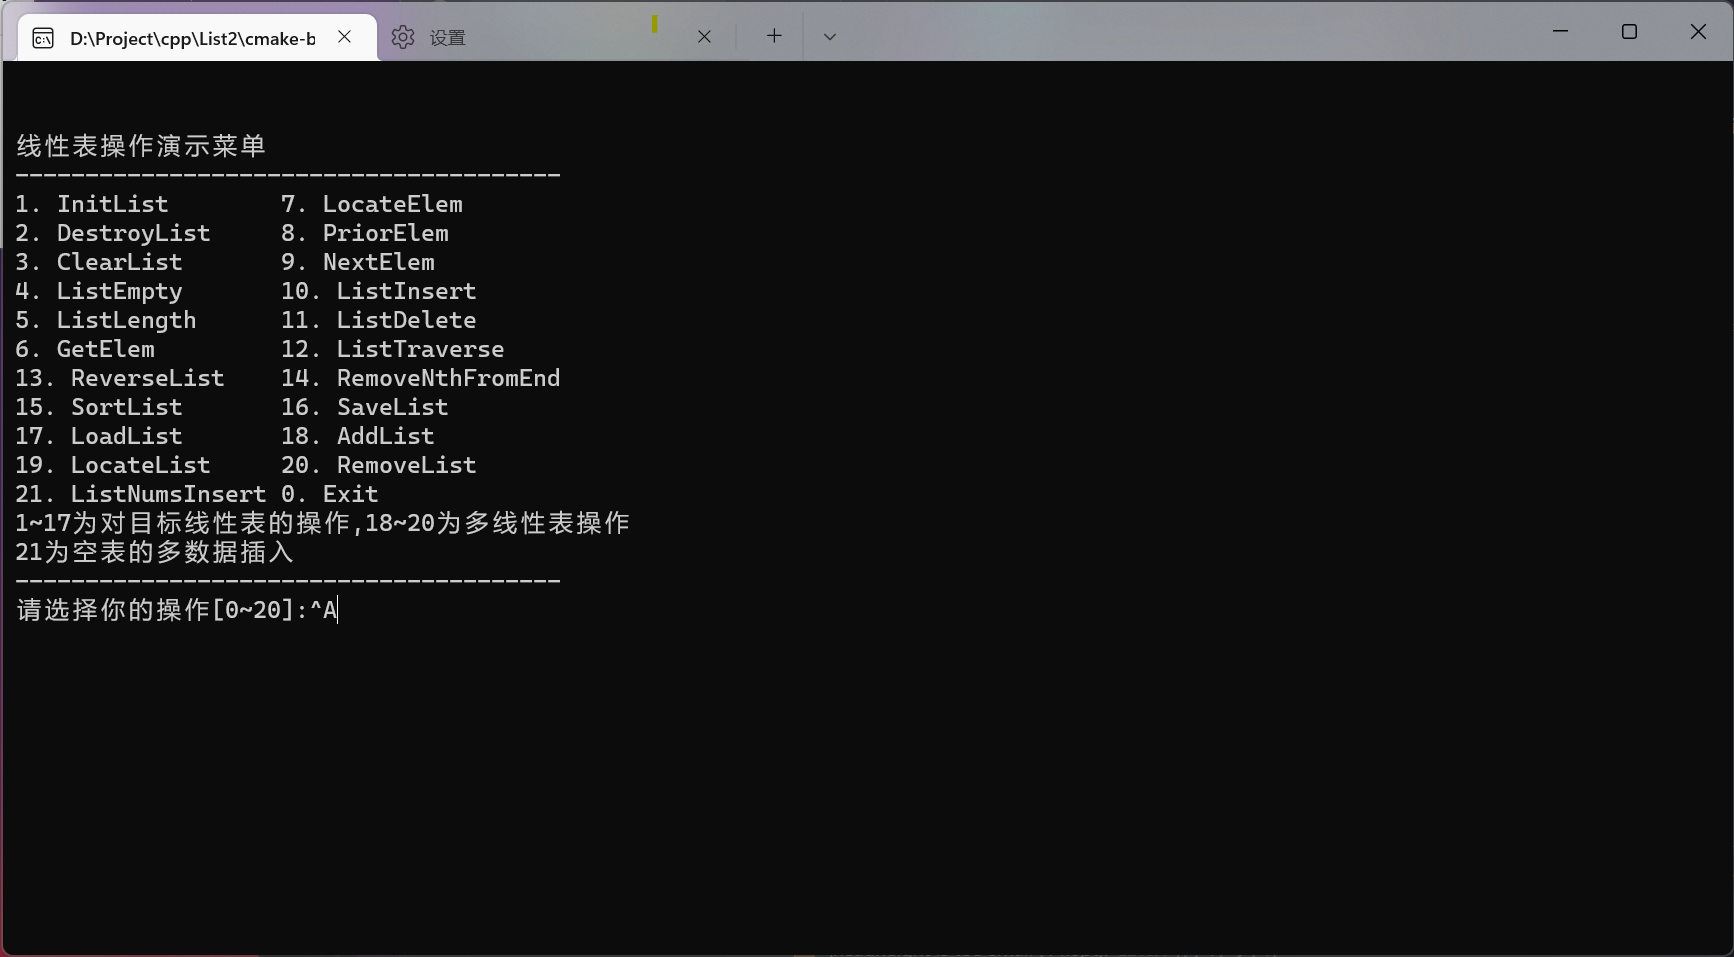
\includegraphics[scale=0.5]{images/p1-1.png}
		\caption{测试界面}
		\label{fig1-1}
	\end{center}
\end{figure}
\subsubsection{测试用例}
链表文件:List(1,4,-2,3,0),NULL(空表),未初始化的表
\newpage
\subsubsection{测试实例}
\begin{enumerate}
	\item InitList测试
	      \begin{table}[htb]
		      \begin{center}
			      \setlength{\tabcolsep}{2.0mm}
			      \caption{InitList测试用例表}
			      \label{table12}
			      \begin{tabular}{|c|c|c|c|}
				      \hline
				      测试用例   & 输入    & 理论结果       & 测试结果       \\
				      \hline
				      \hline
				      List       & 界面选1 & 线性表创建失败 & 线性表创建失败 \\
				      \hline
				      未初始化表 & 界面选1 & 线性表创建成功 & 线性表创建成功 \\
				      \hline
			      \end{tabular}
		      \end{center}
	      \end{table}
	      \begin{figure}[htb]
		      \centering
		      \subfloat[未初始化表测试图]{\label{fig1-20}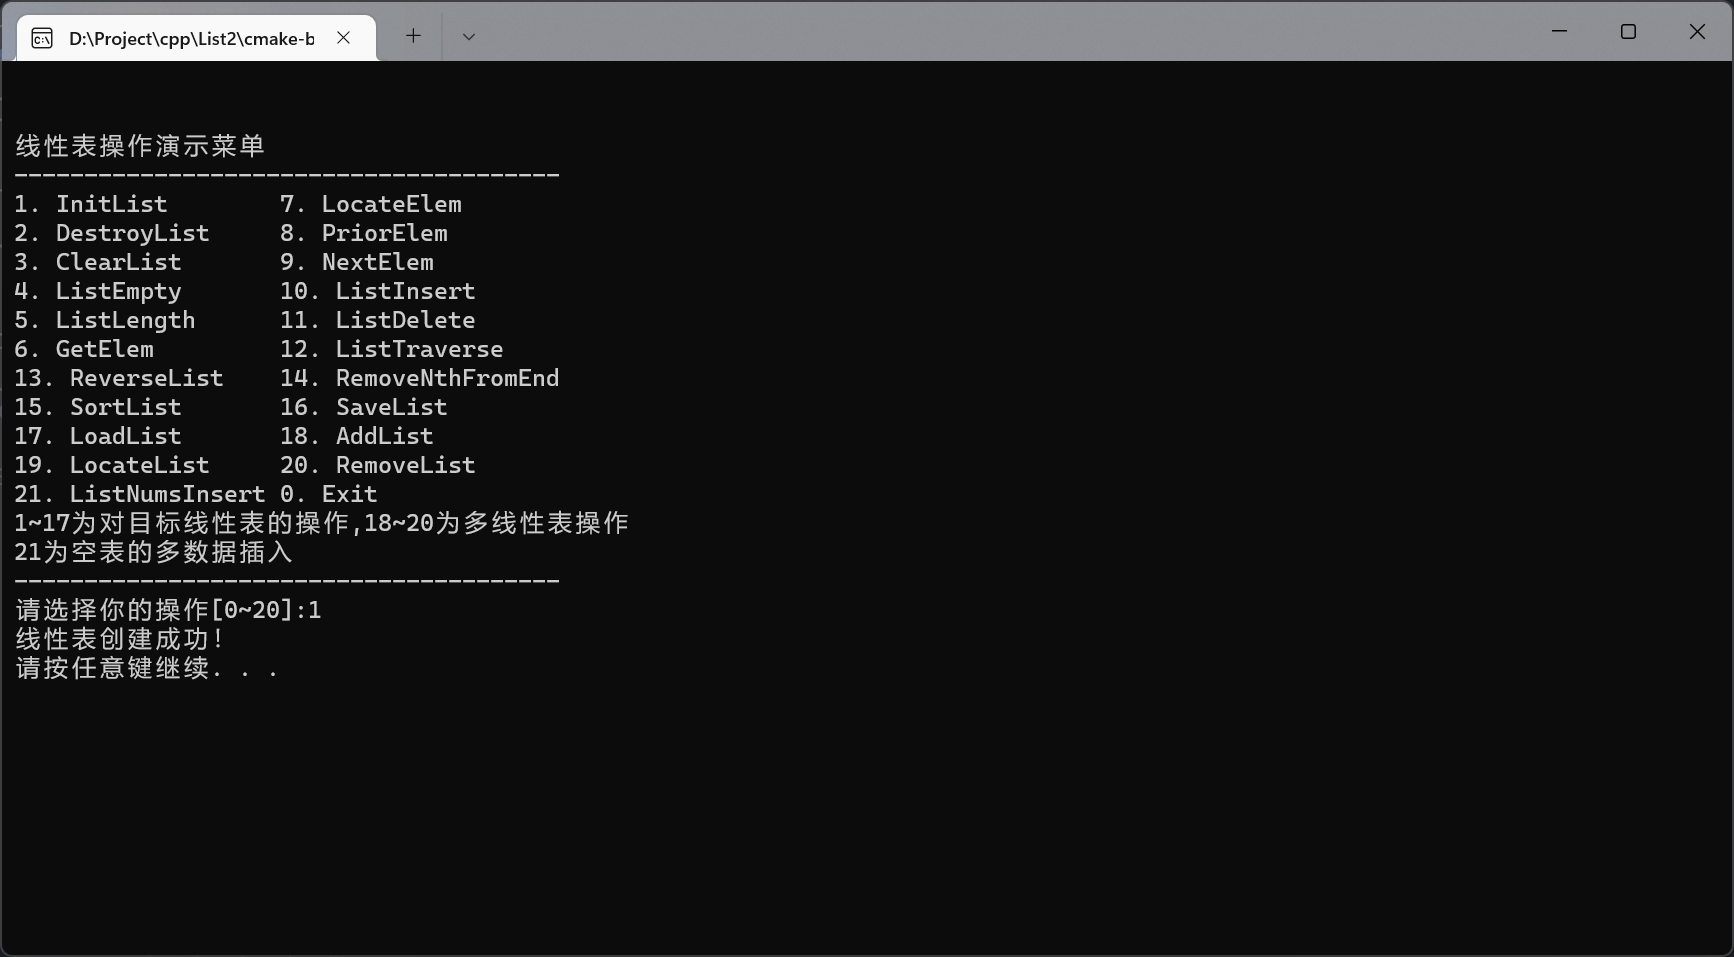
\includegraphics[width=12cm]{images/p1-22.png}}\quad
		      \subfloat[测试用例测试图]{\label{fig1-21}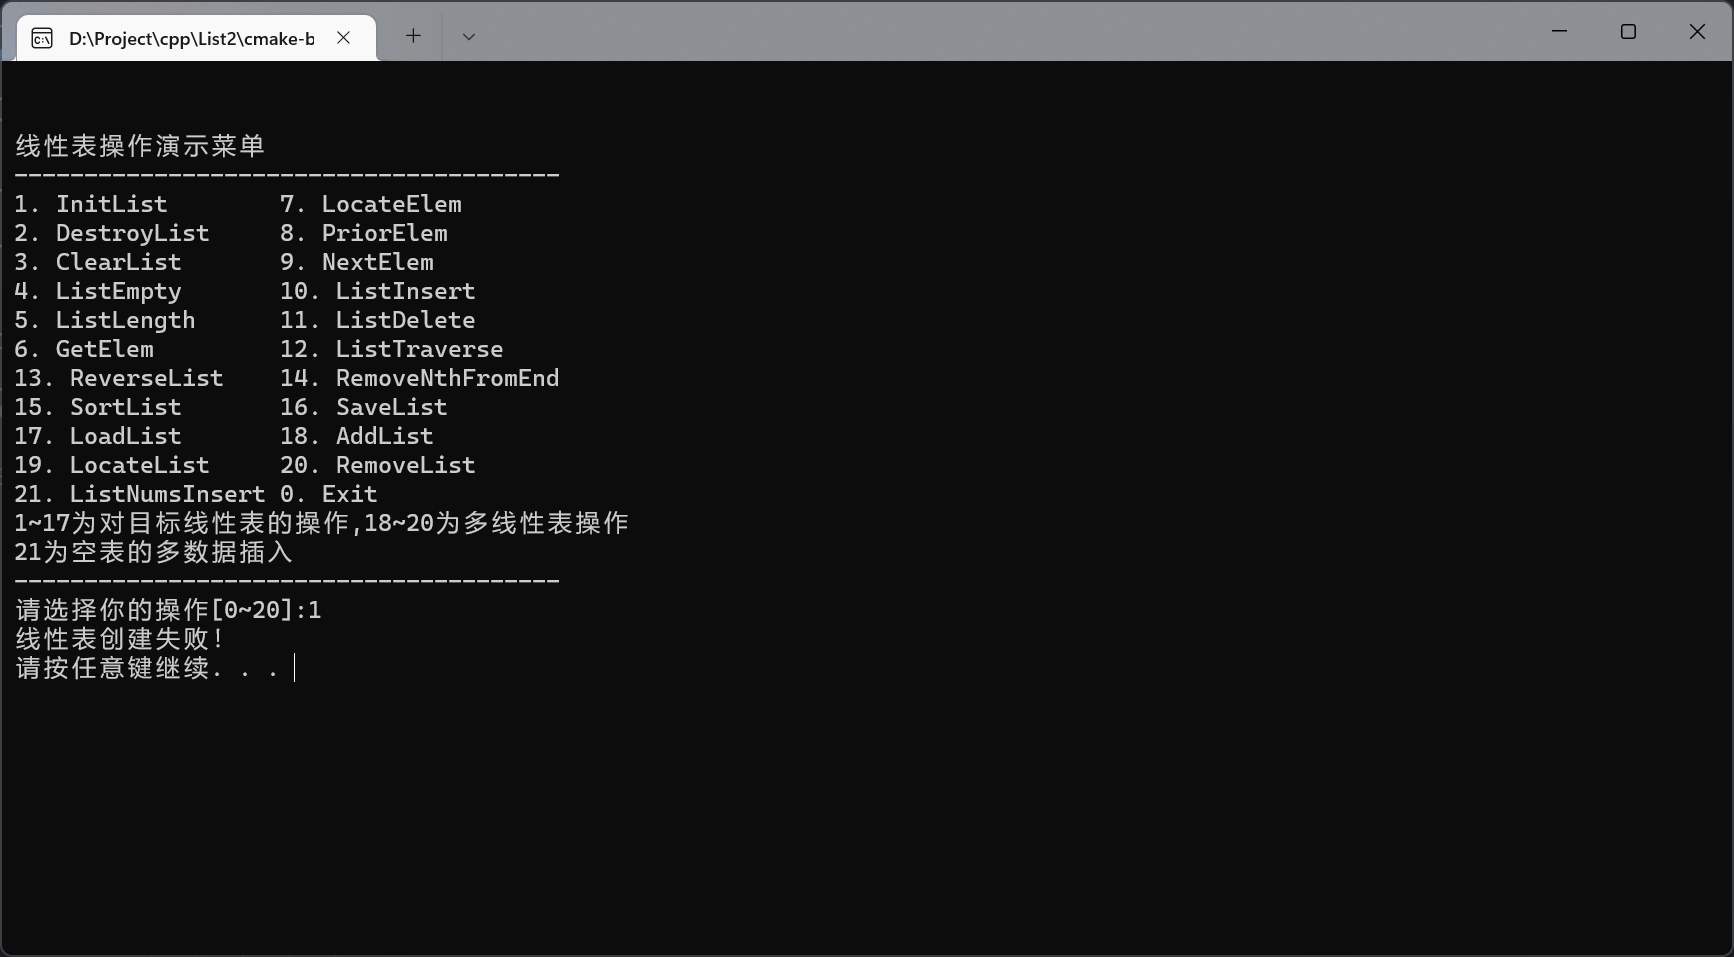
\includegraphics[width=12cm]{images/p1-21.png}}\\
		      \caption{初始化表测试}
	      \end{figure}
	      \newpage
	\item DestroyList测试
	      \begin{table}[htb]
		      \begin{center}
			      \setlength{\tabcolsep}{2.0mm}
			      \caption{DestroyList测试用例表}
			      \label{table13}
			      \begin{tabular}{|c|c|c|c|}
				      \hline
				      测试用例   & 输入    & 理论结果       & 测试结果       \\
				      \hline
				      \hline
				      未初始化表 & 界面选2 & 线性表删除失败 & 线性表删除失败 \\
				      \hline
				      List       & 界面选2 & 线性表删除成功 & 线性表删除成功 \\
				      \hline
			      \end{tabular}
		      \end{center}
	      \end{table}
	      \begin{figure}[htb]
		      \centering
		      \subfloat[未初始化表测试图]{\label{fig1-23}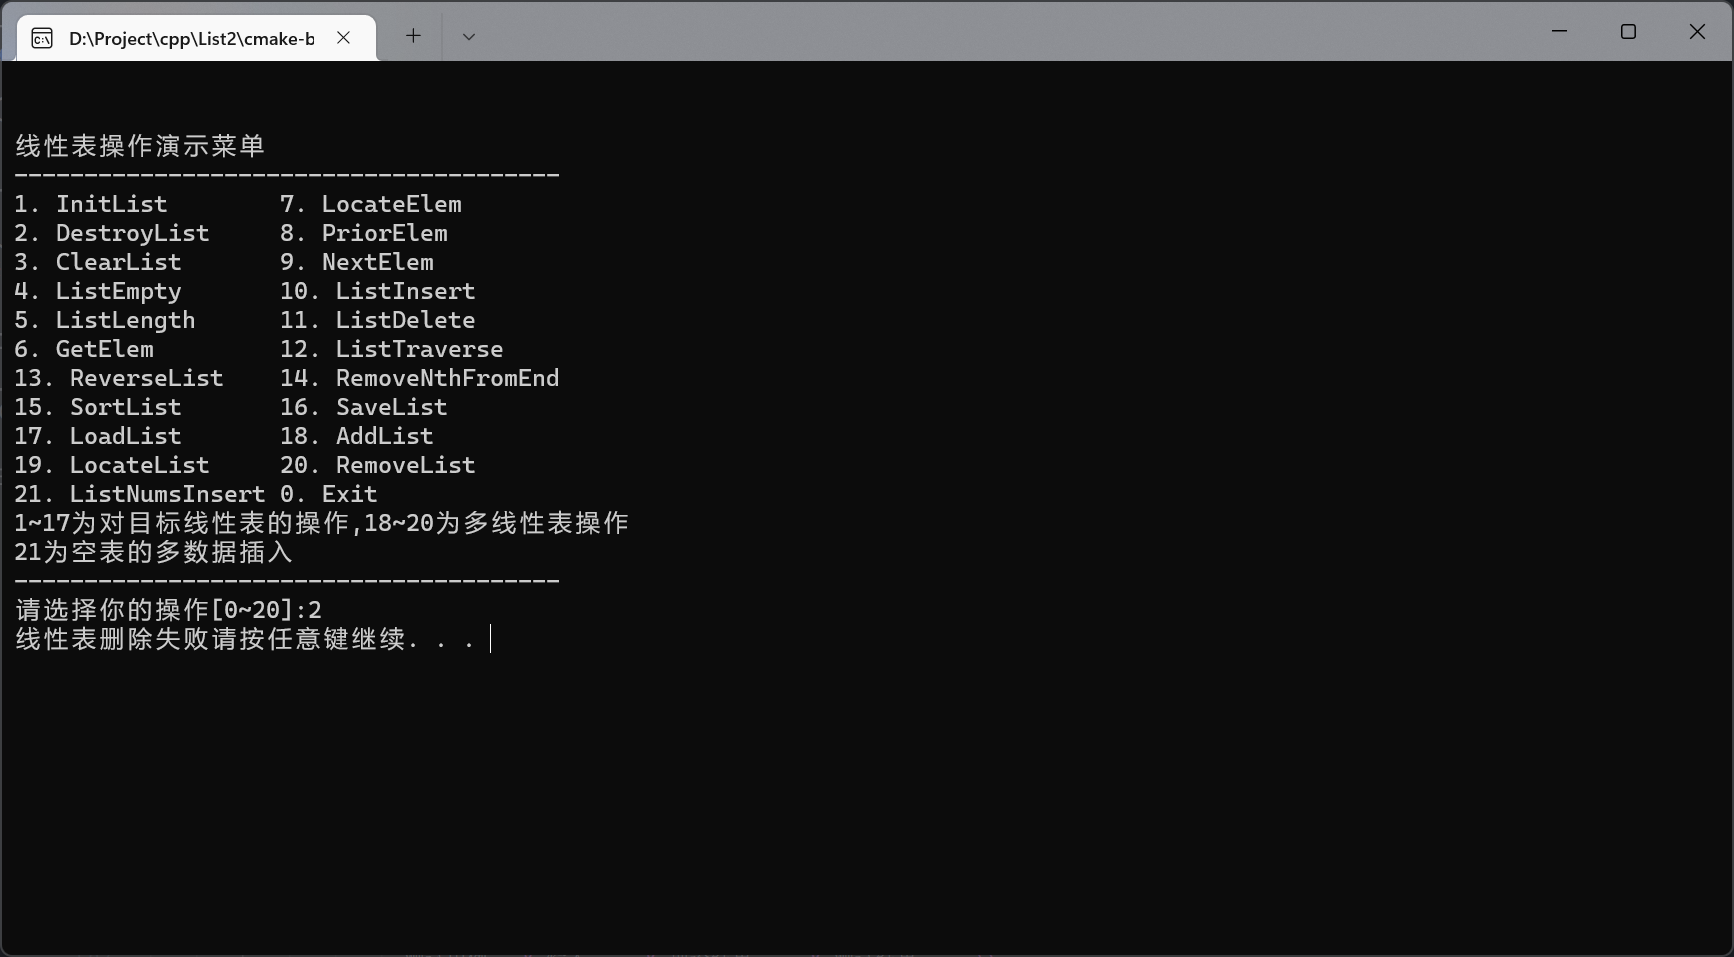
\includegraphics[width=12cm]{images/p1-24.png}}\quad
		      \subfloat[测试用例测试图]{\label{fig1-22}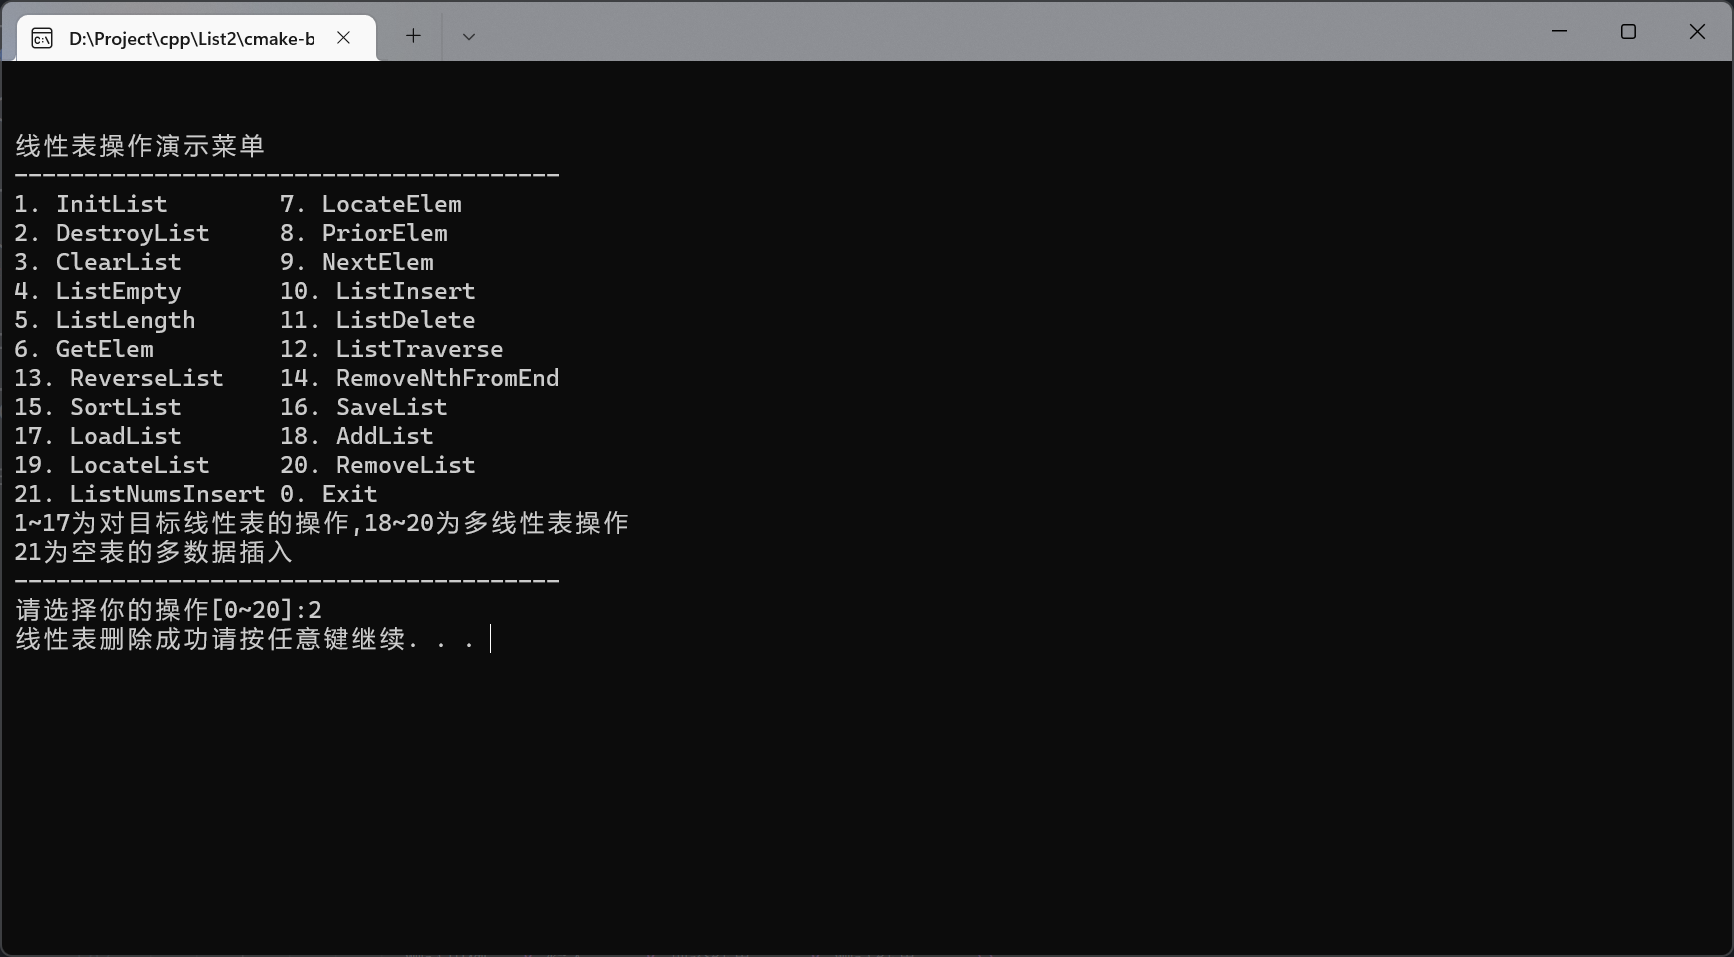
\includegraphics[width=12cm]{images/p1-23.png}}\\
		      \caption{销毁表测试}
	      \end{figure}
	      \newpage
	\item ClearList测试
	      \begin{table}[htb]
		      \begin{center}
			      \setlength{\tabcolsep}{2.0mm}
			      \caption{ClearList测试用例表}
			      \label{table14}
			      \begin{tabular}{|c|c|c|c|}
				      \hline
				      测试用例   & 输入    & 理论结果       & 测试结果       \\
				      \hline
				      \hline
				      未初始化表 & 界面选3 & 线性表不存在   & 线性表不存在   \\
				      \hline
				      List       & 界面选3 & 线性表清空成功 & 线性表清空成功 \\
				      \hline
				      NULL       & 界面选3 & 线性表为空     & 线性表为空     \\
				      \hline
			      \end{tabular}
		      \end{center}
	      \end{table}
	      \begin{figure}[htb]
		      \centering
		      \subfloat[NULL表测试图]{\label{fig1-24}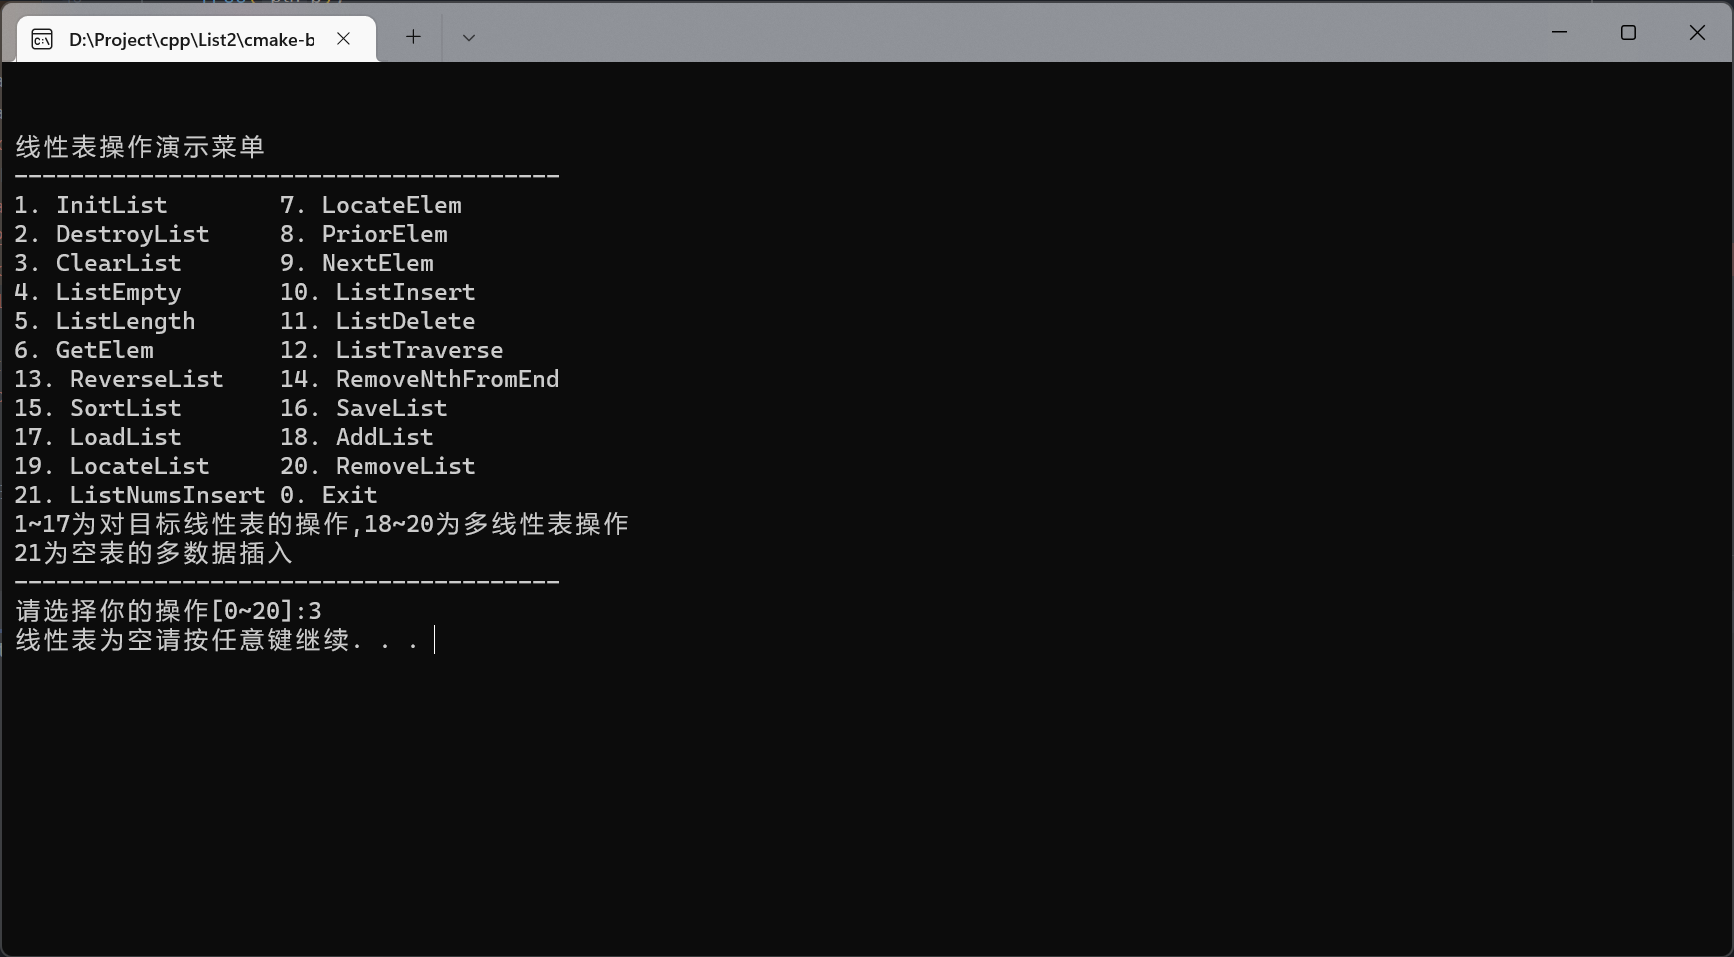
\includegraphics[width=7cm]{images/p1-25.png}}\quad
		      \subfloat[未初始化表测试图]{\label{fig1-25}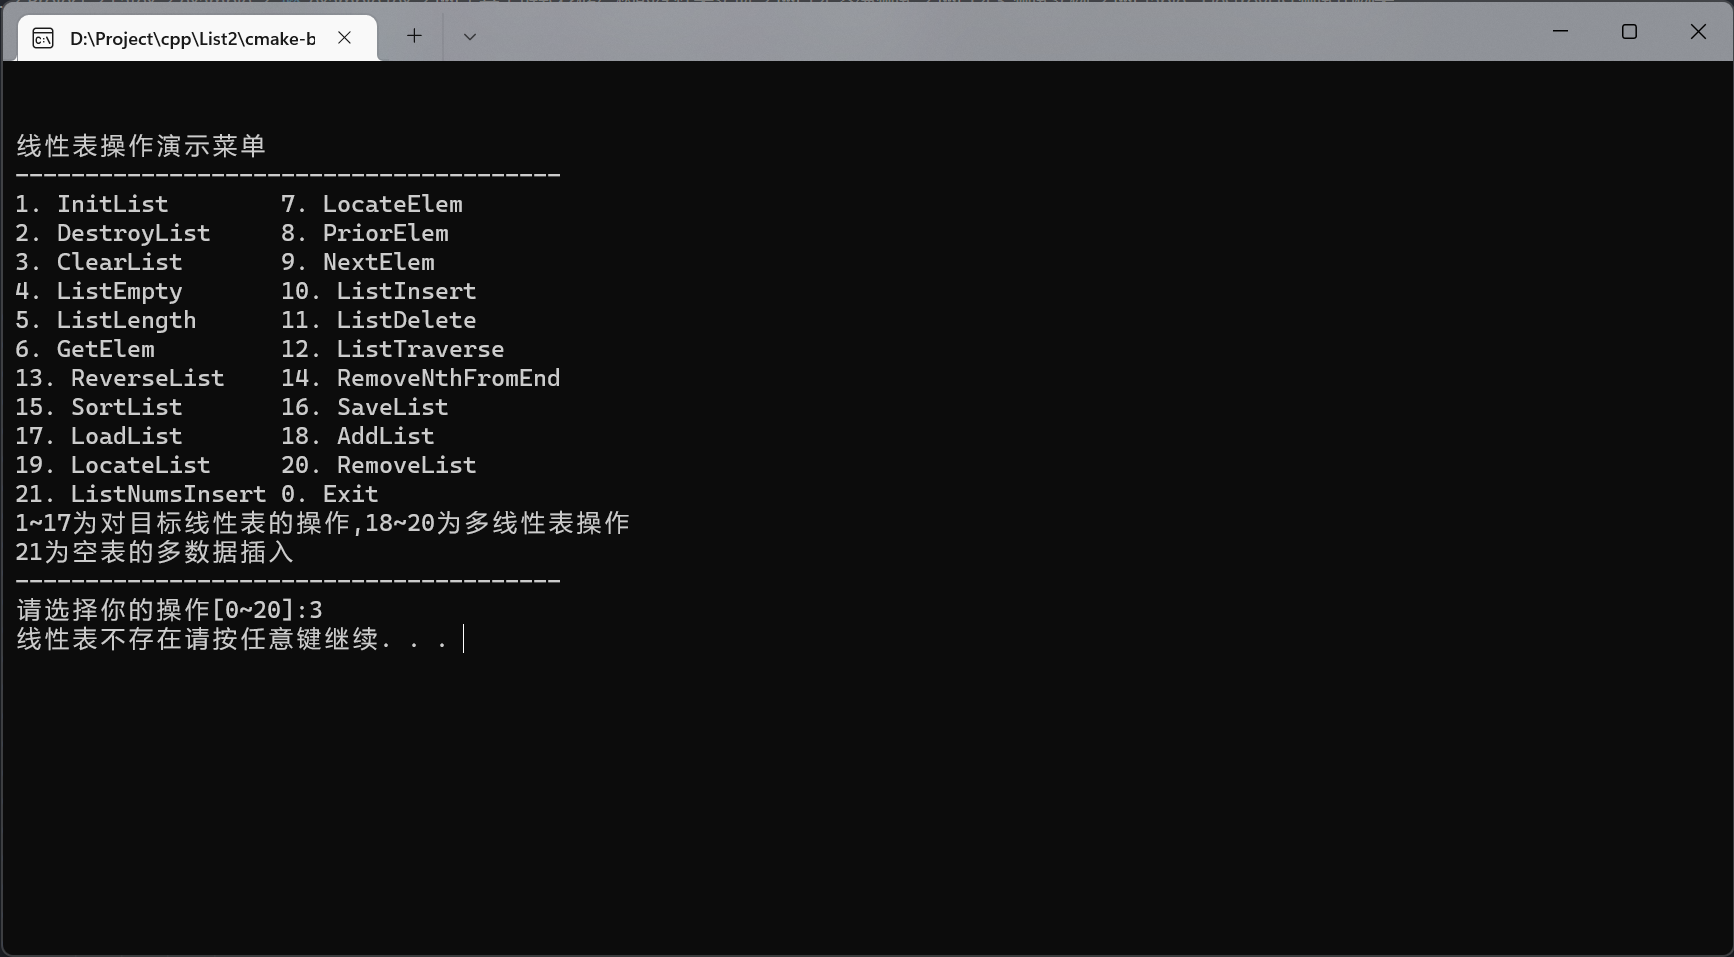
\includegraphics[width=7cm]{images/p1-26.png}}\quad
		      \subfloat[测试用例测试图]{\label{fig1-26}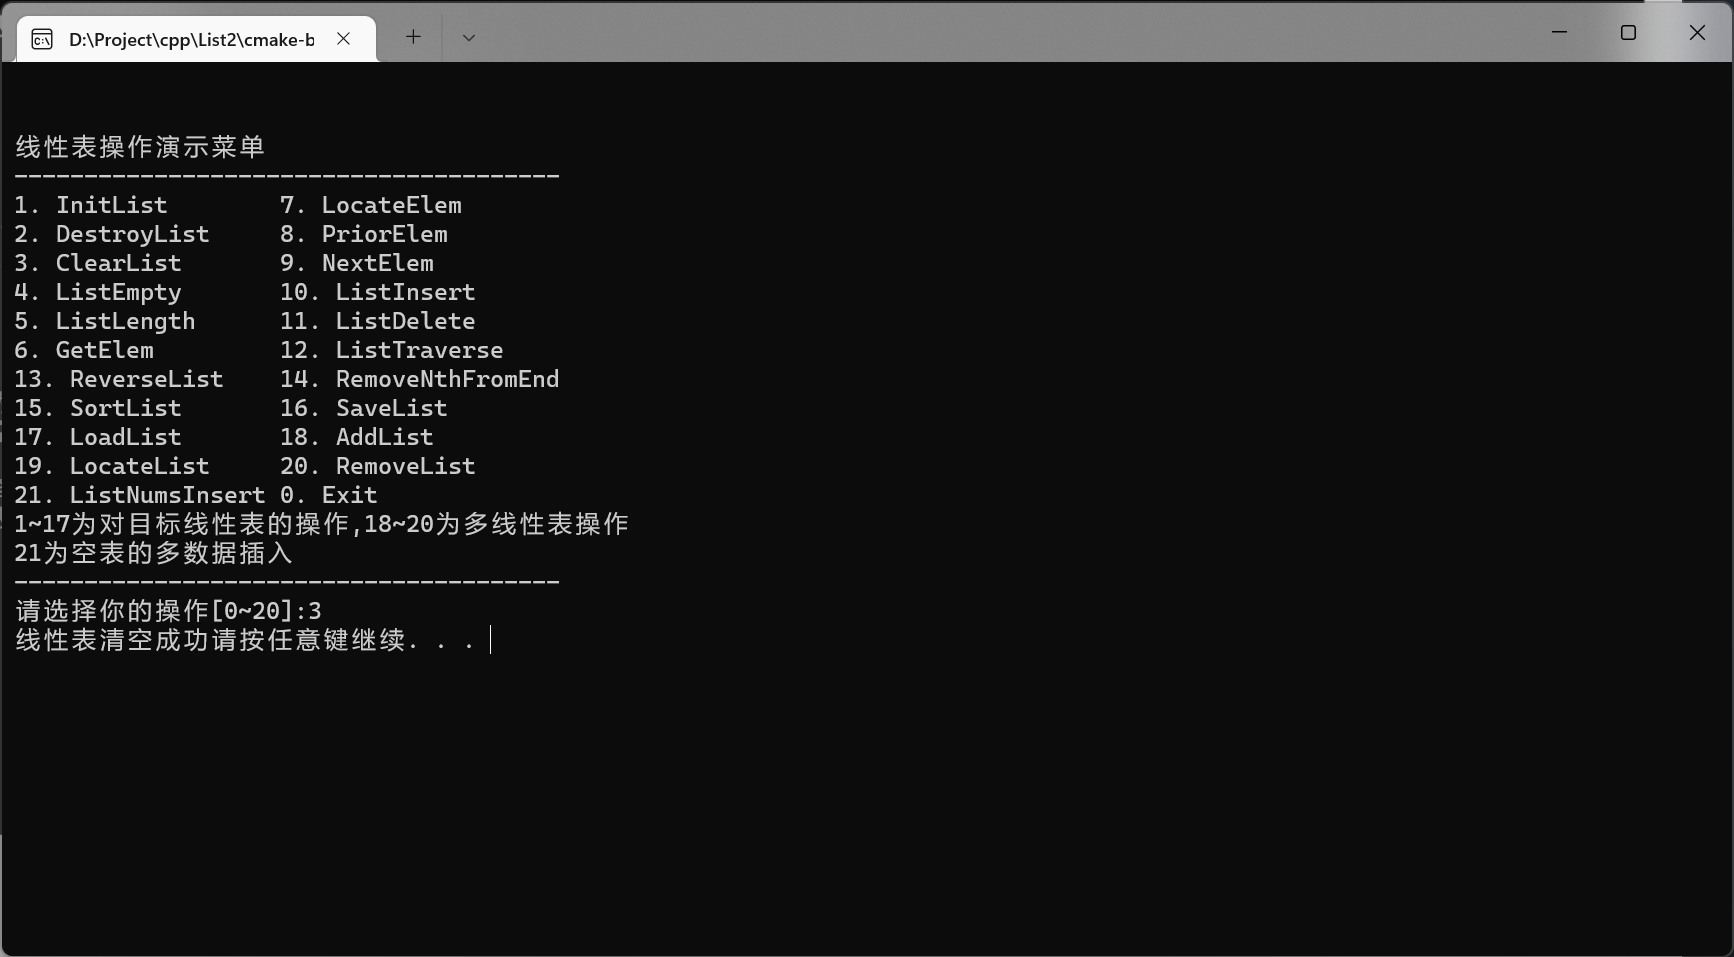
\includegraphics[width=12cm]{images/p1-27.png}}\\
		      \caption{清空表测试}
	      \end{figure}
	      \newpage
	\item ListEmpty测试
	      \begin{table}[htb]
		      \begin{center}
			      \setlength{\tabcolsep}{2.0mm}
			      \caption{ListEmpty测试用例表}
			      \label{table3}
			      \begin{tabular}{|c|c|c|c|}
				      \hline
				      测试用例   & 输入    & 理论结果     & 测试结果     \\
				      \hline
				      \hline
				      List       & 界面选4 & 线性表不为空 & 线性表不为空 \\
				      \hline
				      NULL       & 界面选4 & 线性表为空   & 线性表为空   \\
				      \hline
				      未初始化表 & 界面选4 & 线性表不存在 & 线性表不存在 \\
				      \hline
			      \end{tabular}
		      \end{center}
	      \end{table}
	      \begin{figure}[htb] % here top bottom
		      \begin{center}
			      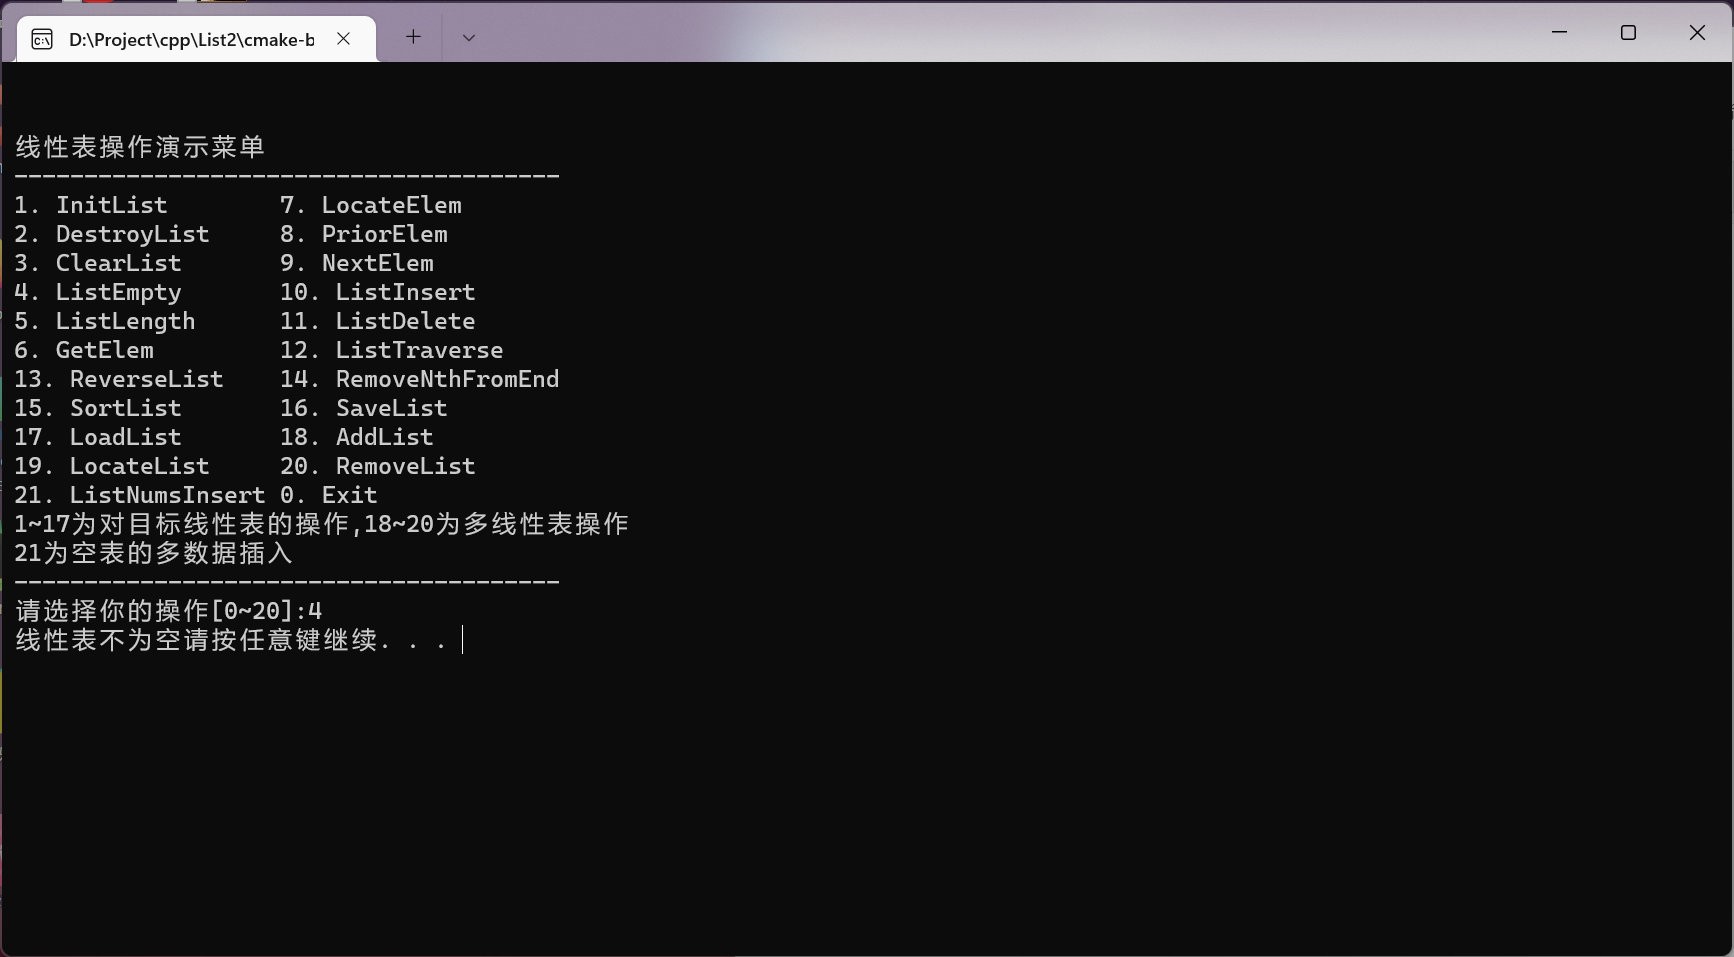
\includegraphics[scale=0.5]{images/p1-2.png}
			      \caption{链表判空界面}
			      \label{fig1-2}
		      \end{center}
	      \end{figure}
	\item ListLength测试
	      \begin{table}[htb]
		      \begin{center}
			      \setlength{\tabcolsep}{2.0mm}
			      \caption{ListLength测试用例表}
			      \label{table4}
			      \begin{tabular}{|c|c|c|c|}
				      \hline
				      测试用例   & 输入    & 理论结果     & 测试结果     \\
				      \hline
				      \hline
				      List       & 界面选5 & 线性表长为5  & 线性表长为5  \\
				      \hline
				      NULL       & 界面选5 & 线性表为空   & 线性表为空   \\
				      \hline
				      未初始化表 & 界面选5 & 线性表不存在 & 线性表不存在 \\
				      \hline
			      \end{tabular}
		      \end{center}
	      \end{table}
	      \newpage
	      \begin{figure}[htb] % here top bottom
		      \begin{center}
			      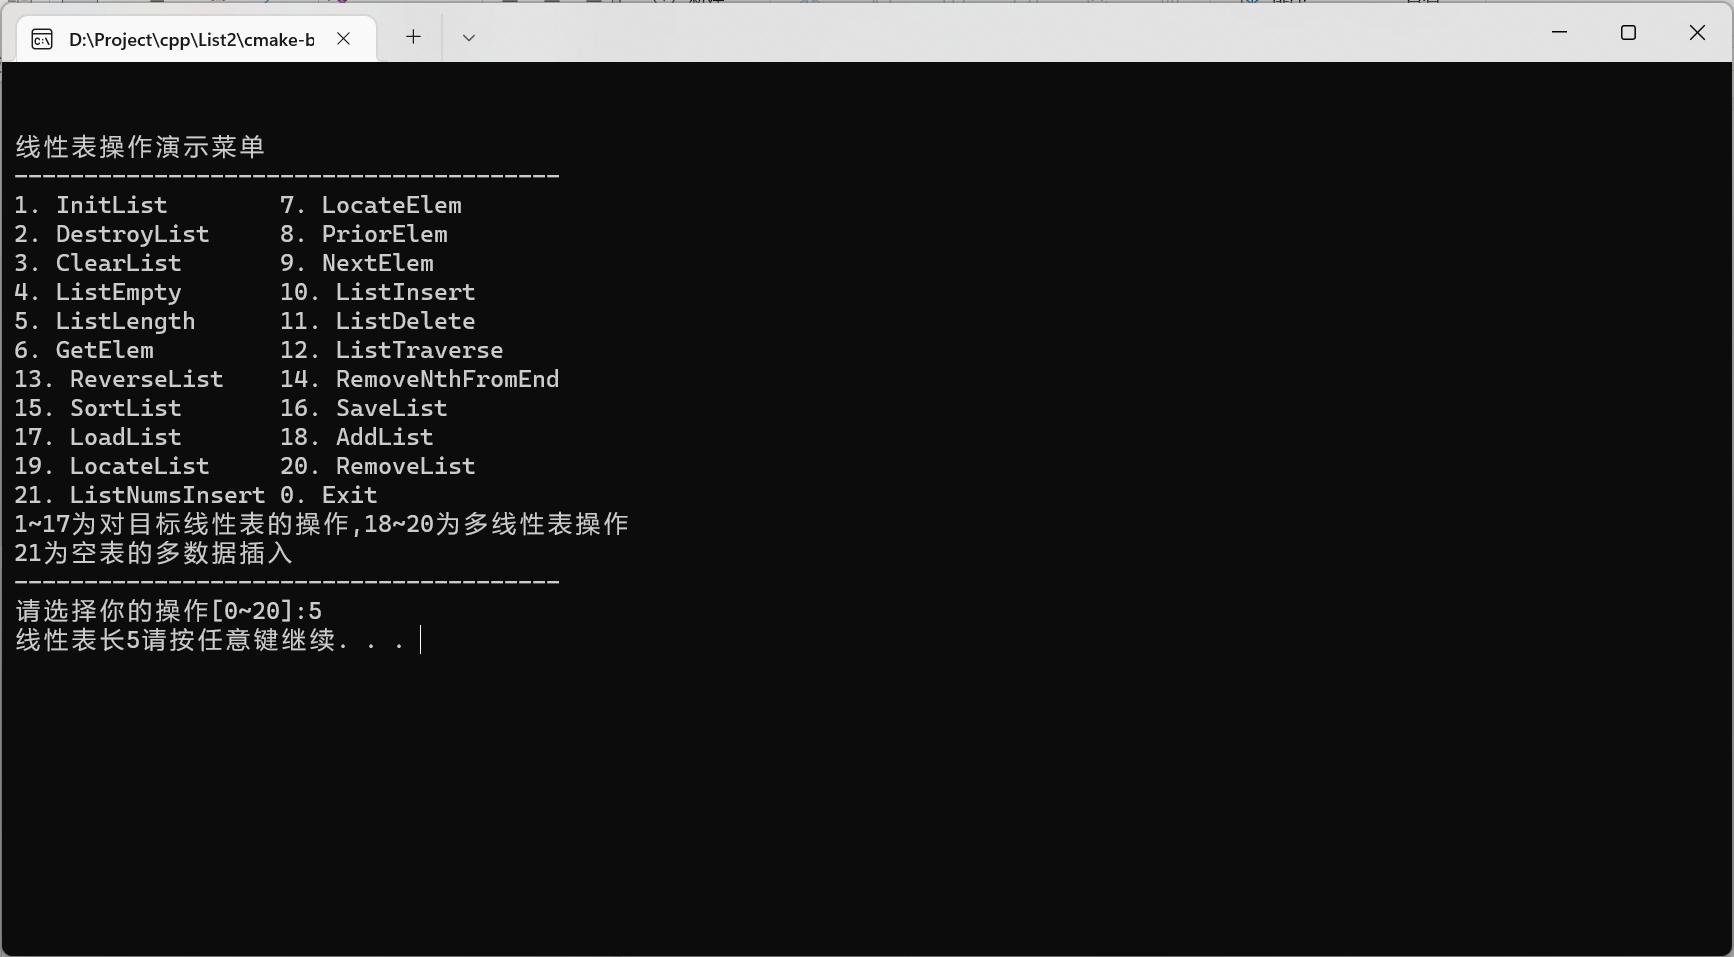
\includegraphics[scale=0.5]{images/p1-3}
			      \caption{获取表长界面}
			      \label{fig1-3}
		      \end{center}
	      \end{figure}
	\item GetElem测试
	      \begin{table}[htb]
		      \begin{center}
			      \setlength{\tabcolsep}{2.0mm}
			      \caption{GetElem测试用例表}
			      \label{table5}
			      \begin{tabular}{|c|c|c|c|}
				      \hline
				      测试用例   & 输入              & 理论结果        & 测试结果        \\
				      \hline
				      \hline
				      List       & 界面选6,输入位置3 & 第三个元素为-2  & 第三个元素为-2  \\
				      \hline
				      List       & 界面选6,输入位置6 & 不存在第6个元素 & 不存在第6个元素 \\
				      \hline
				      未初始化表 & 界面选6           & 线性表不存在    & 线性表不存在    \\
				      \hline
			      \end{tabular}
		      \end{center}
	      \end{table}
	      \begin{figure}[htb]
		      \centering
		      \subfloat[正确节点测试图]{\label{fig1-4}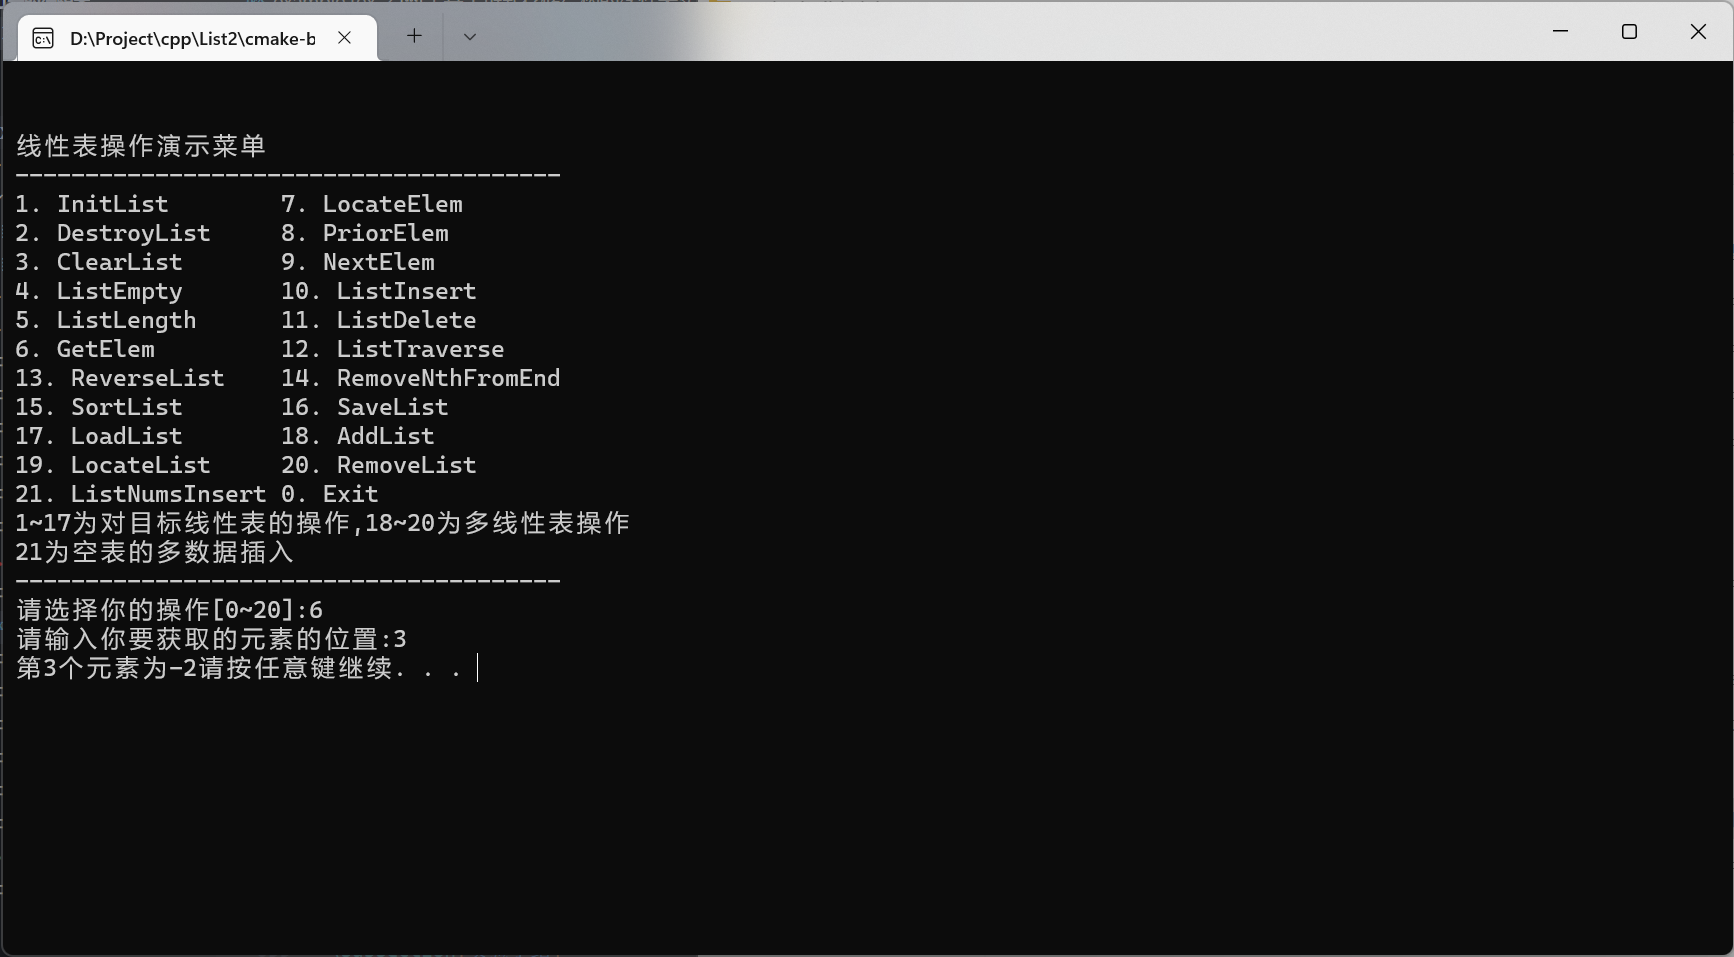
\includegraphics[width=7cm]{images/p1-4.png}}\quad
		      \subfloat[错误节点测试图]{\label{fig1-5}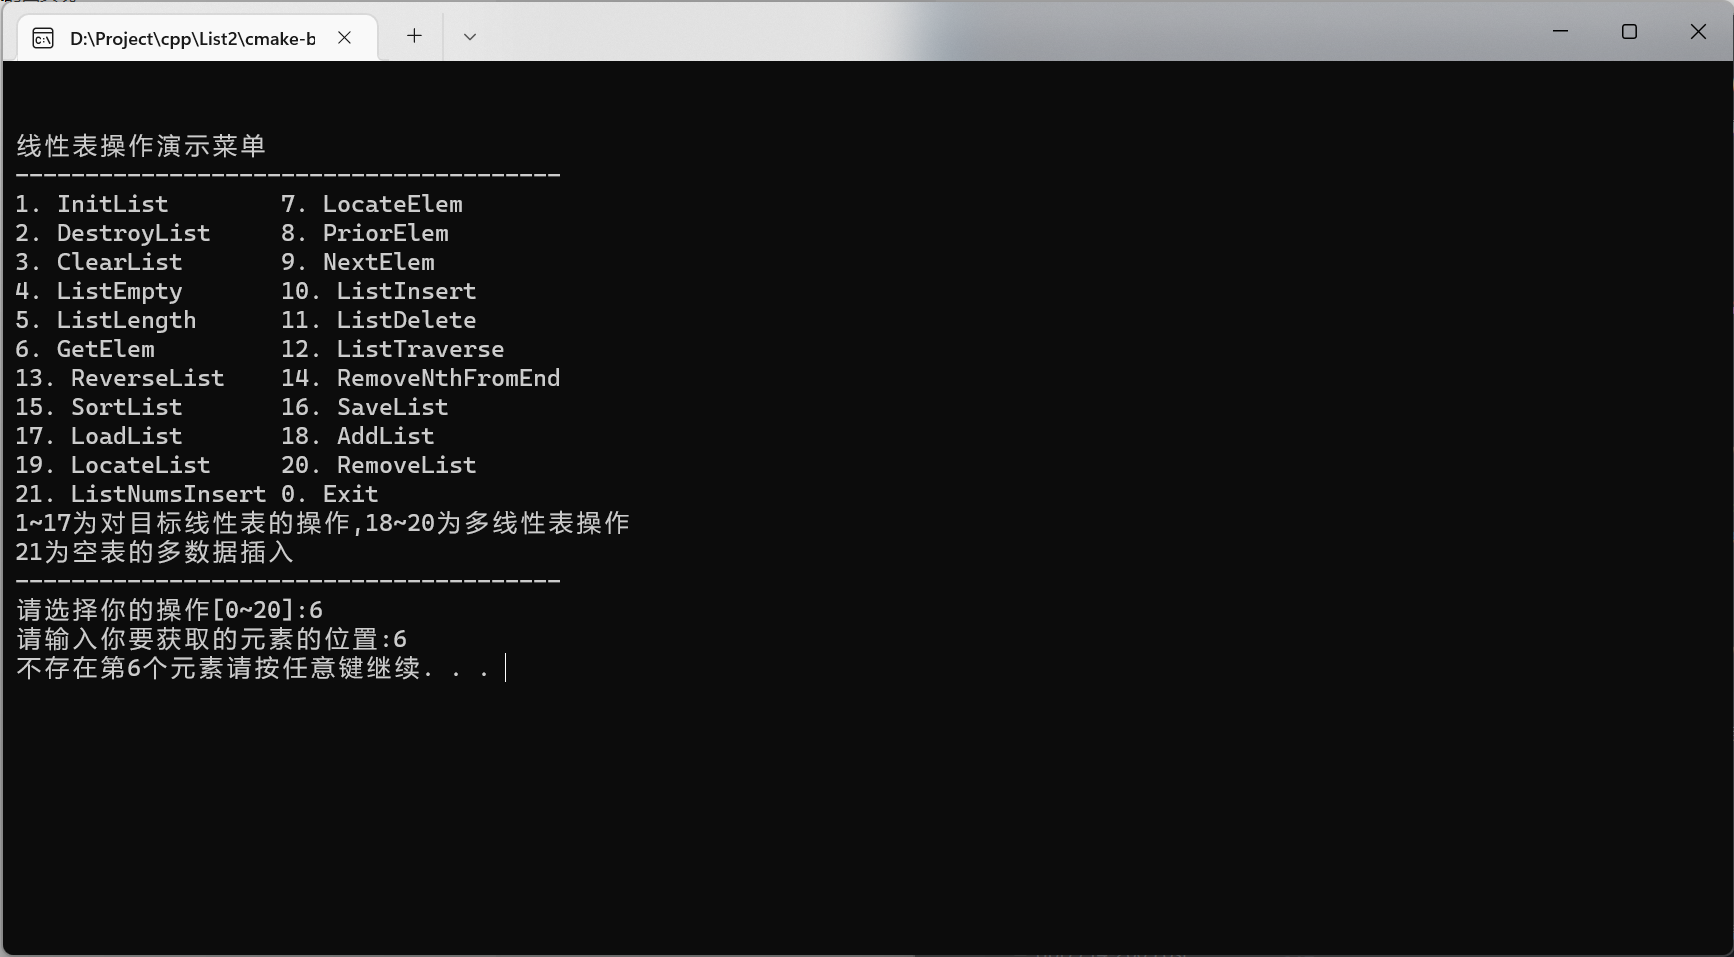
\includegraphics[width=7cm]{images/p1-5.png}}\\
		      \caption{节点测试}
	      \end{figure}
	      \newpage
	\item LocateElem测试
	      \begin{table}[htb]
		      \begin{center}
			      \setlength{\tabcolsep}{2.0mm}
			      \caption{LocateElem测试用例表}
			      \label{table6}
			      \begin{tabular}{|c|c|c|c|}
				      \hline
				      测试用例   & 输入              & 理论结果           & 测试结果           \\
				      \hline
				      \hline
				      List       & 界面选7,输入位置4 & 元素4位于第2个位置 & 元素4位于第2个位置 \\
				      \hline
				      List       & 界面选7,输入位置7 & 不存在为7的元素    & 不存在为7的元素    \\
				      \hline
				      未初始化表 & 界面选7           & 线性表不存在       & 线性表不存在       \\
				      \hline
			      \end{tabular}
		      \end{center}
	      \end{table}
	      \begin{figure}[htb]
		      \centering
		      \subfloat[正确元素测试图]{\label{fig1-6}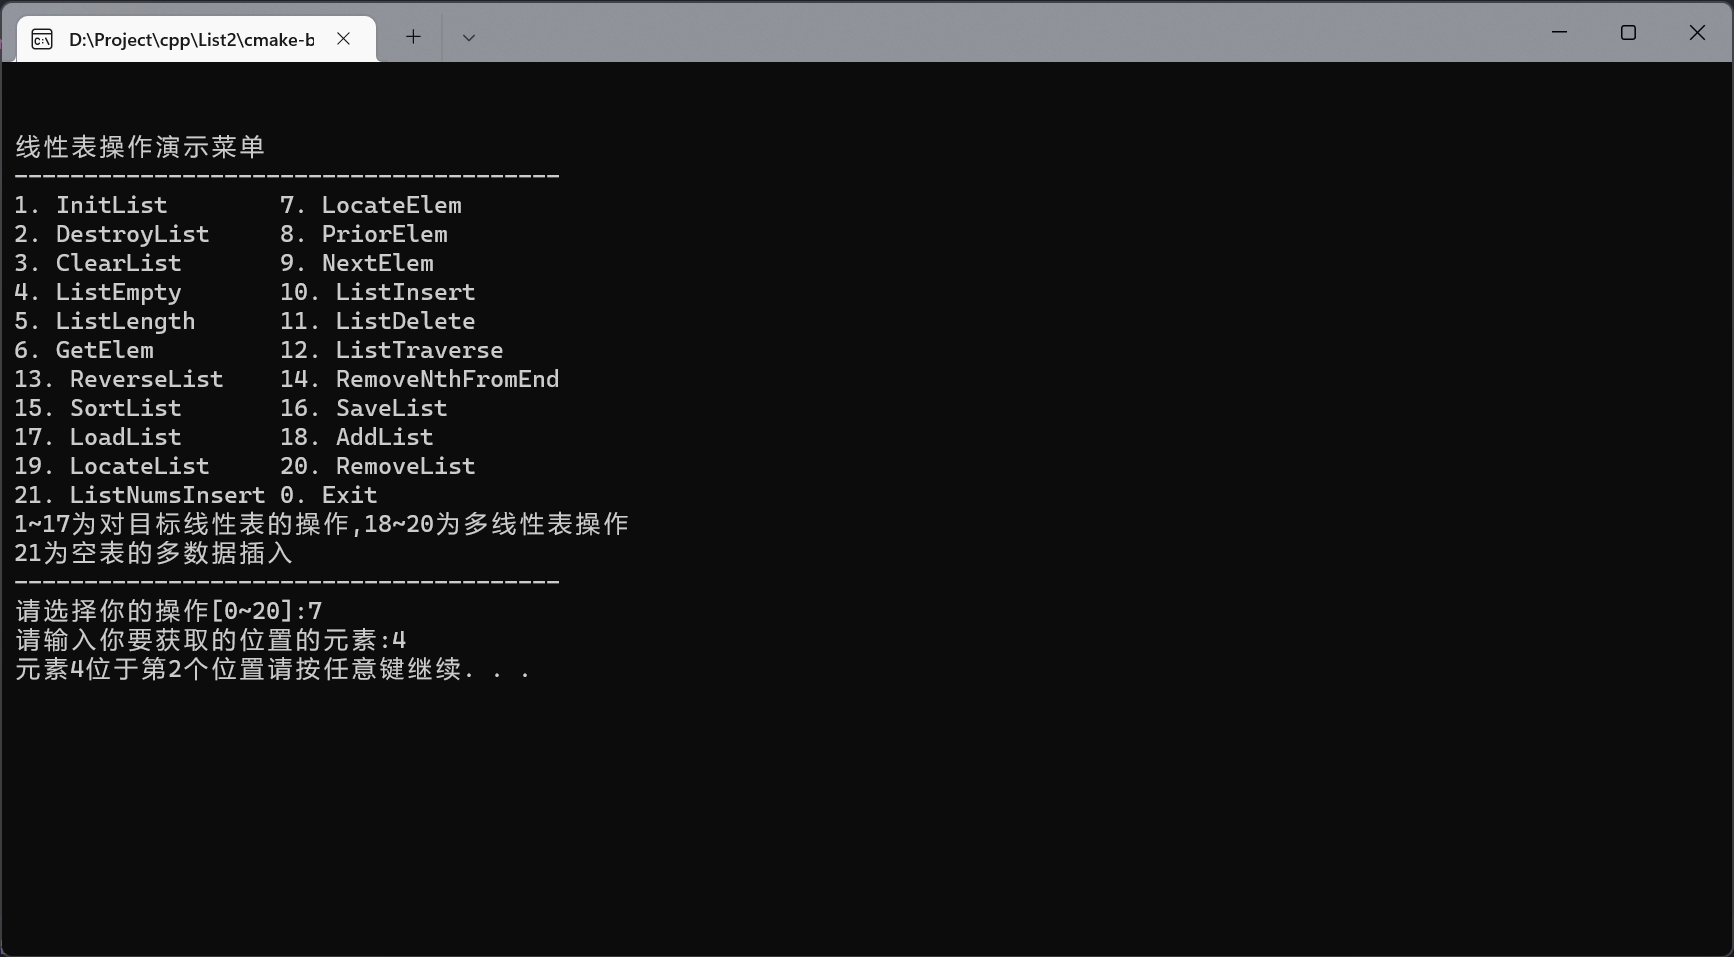
\includegraphics[width=12cm]{images/p1-7}}\quad
		      \subfloat[错误元素测试图]{\label{fig1-7}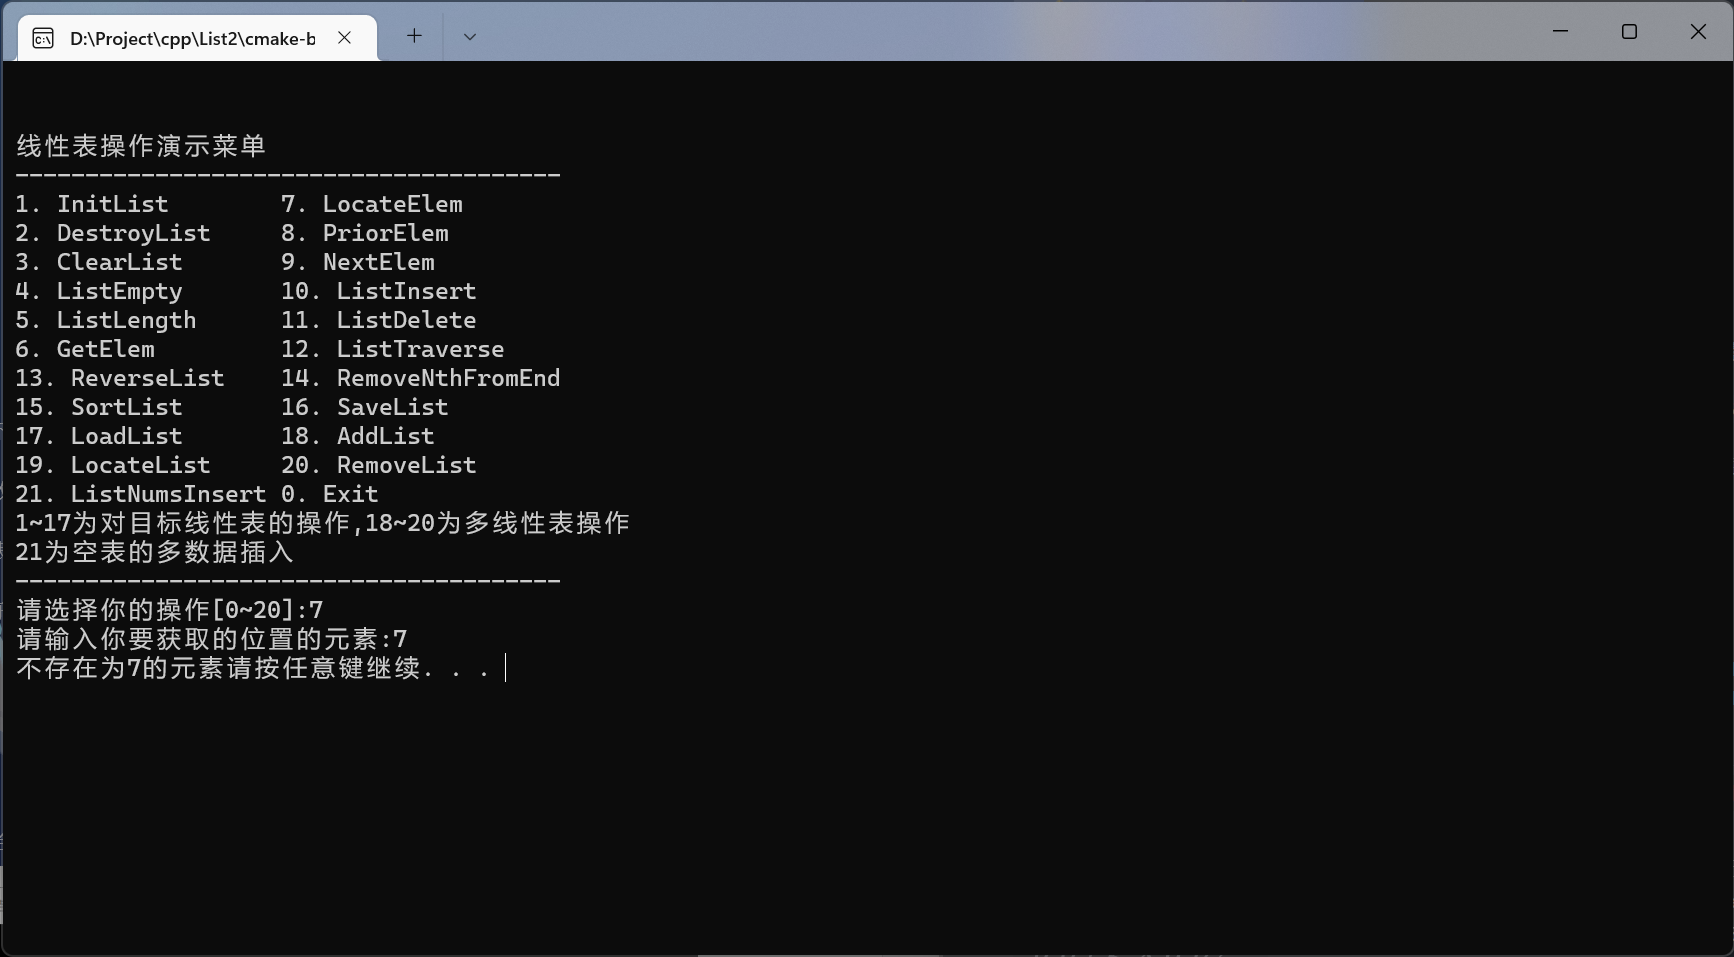
\includegraphics[width=12cm]{images/p1-8}}\\
		      \caption{元素测试}
	      \end{figure}
	      \newpage
	\item PriorElem测试
	      \begin{table}[htb]
		      \begin{center}
			      \setlength{\tabcolsep}{2.0mm}
			      \caption{PriorElem测试用例表}
			      \label{table7}
			      \begin{tabular}{|c|c|c|c|}
				      \hline
				      测试用例   & 输入               & 理论结果              & 测试结果              \\
				      \hline
				      \hline
				      List       & 界面选8,输入位置-2 & 元素-2的前驱元素为4   & 元素-2的前驱元素为:4  \\
				      \hline
				      List       & 界面选8,输入位置1  & 不存在元素1的前驱元素 & 不存在元素1的前驱元素 \\
				      \hline
				      List       & 界面选8,输入位置13 & 线性表不存在元素13    & 线性表不存在元素13    \\
				      \hline
				      未初始化表 & 界面选8            & 线性表不存在          & 线性表不存在          \\
				      \hline
			      \end{tabular}
		      \end{center}
	      \end{table}
	      \begin{figure}[htb]
		      \centering
		      \subfloat[正确元素测试图]{\label{fig1-8}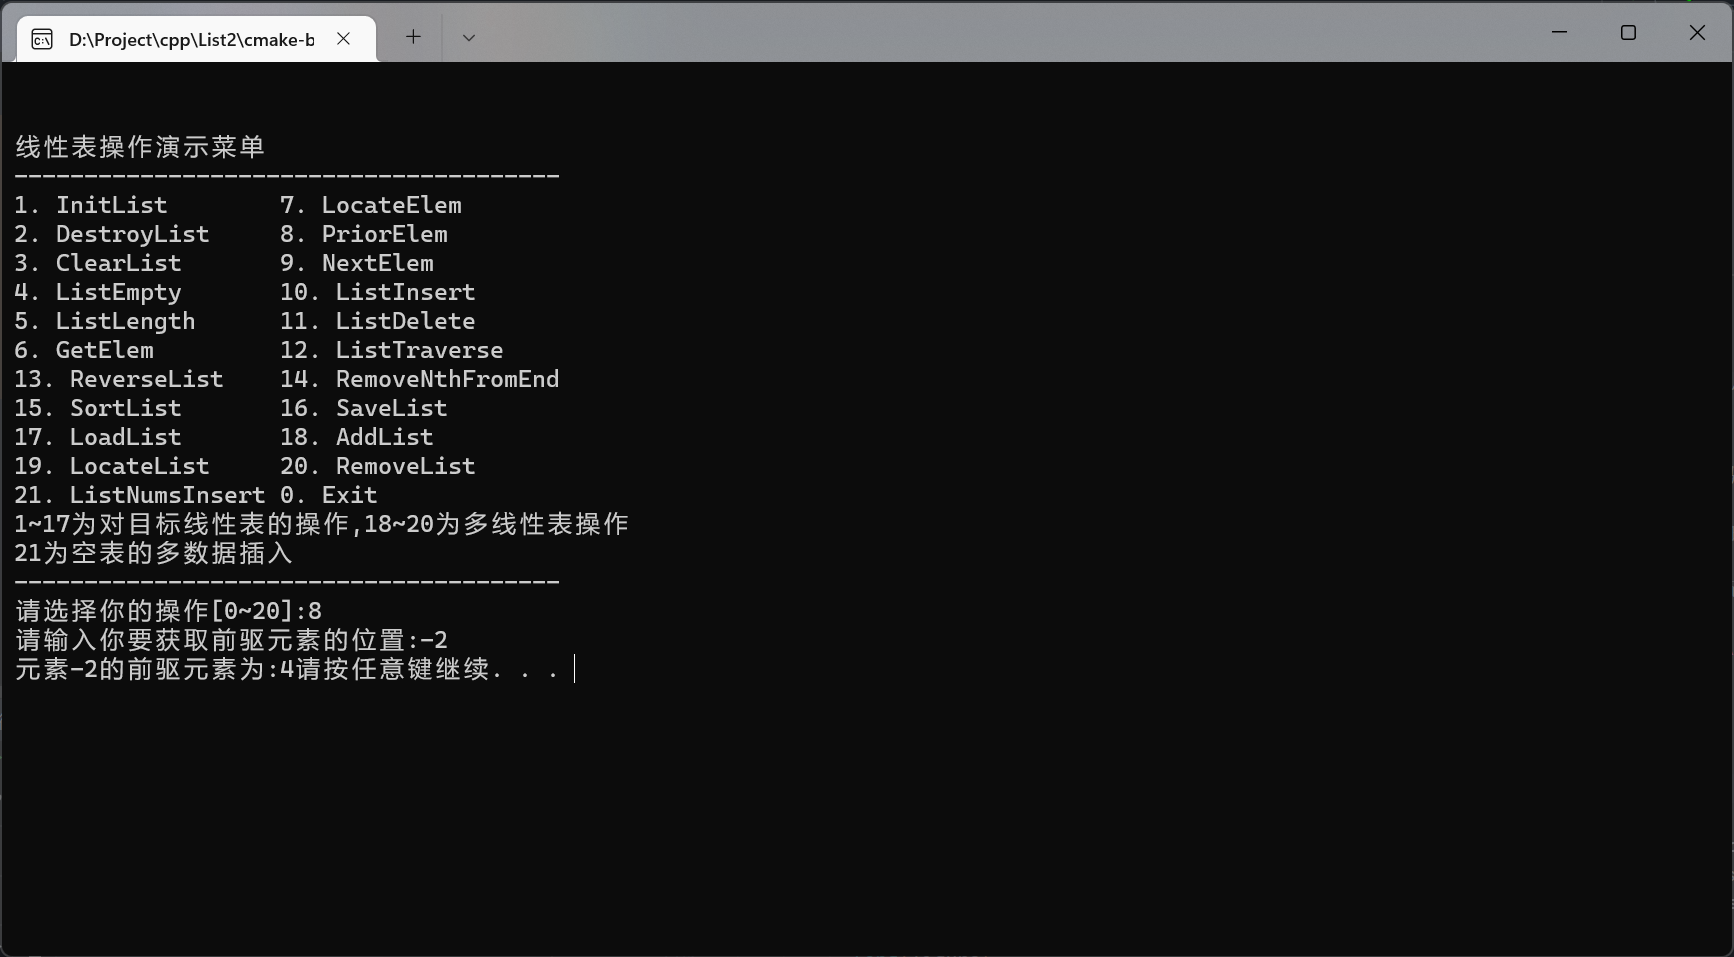
\includegraphics[width=7cm]{images/p1-9.png}}\quad
		      \subfloat[首位置元素测试图]{\label{fig1-9}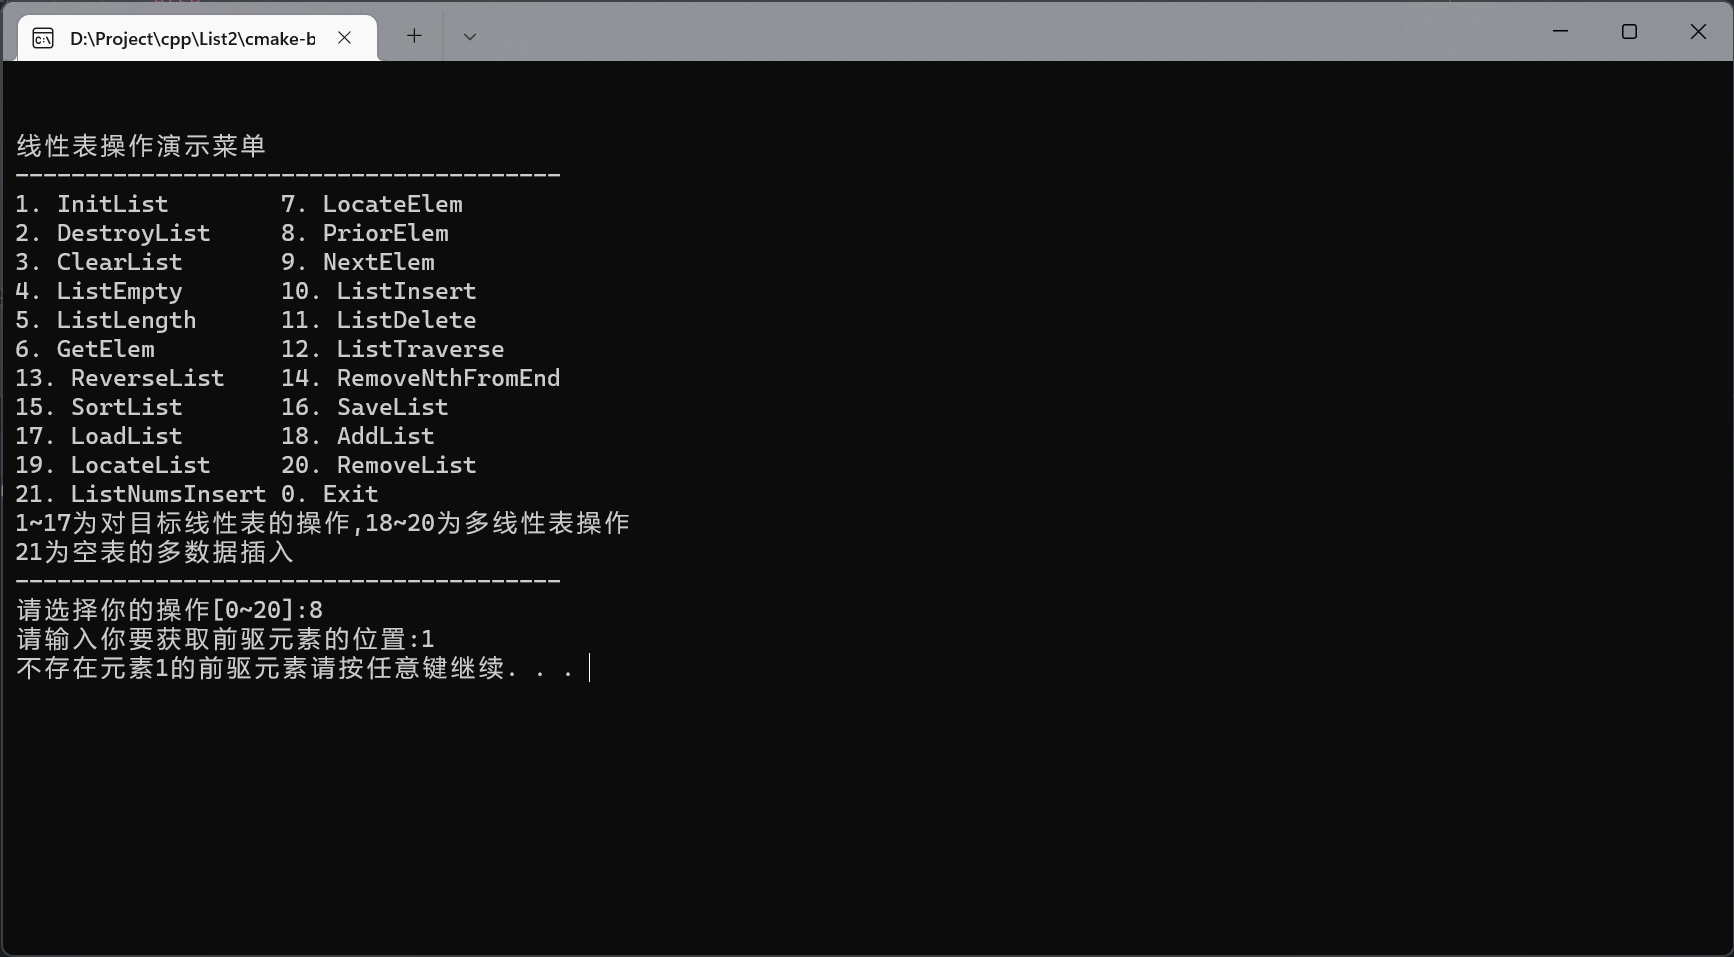
\includegraphics[width=7cm]{images/p1-10.png}}\quad
		      \subfloat[错误元素测试图]{\label{fig1-10}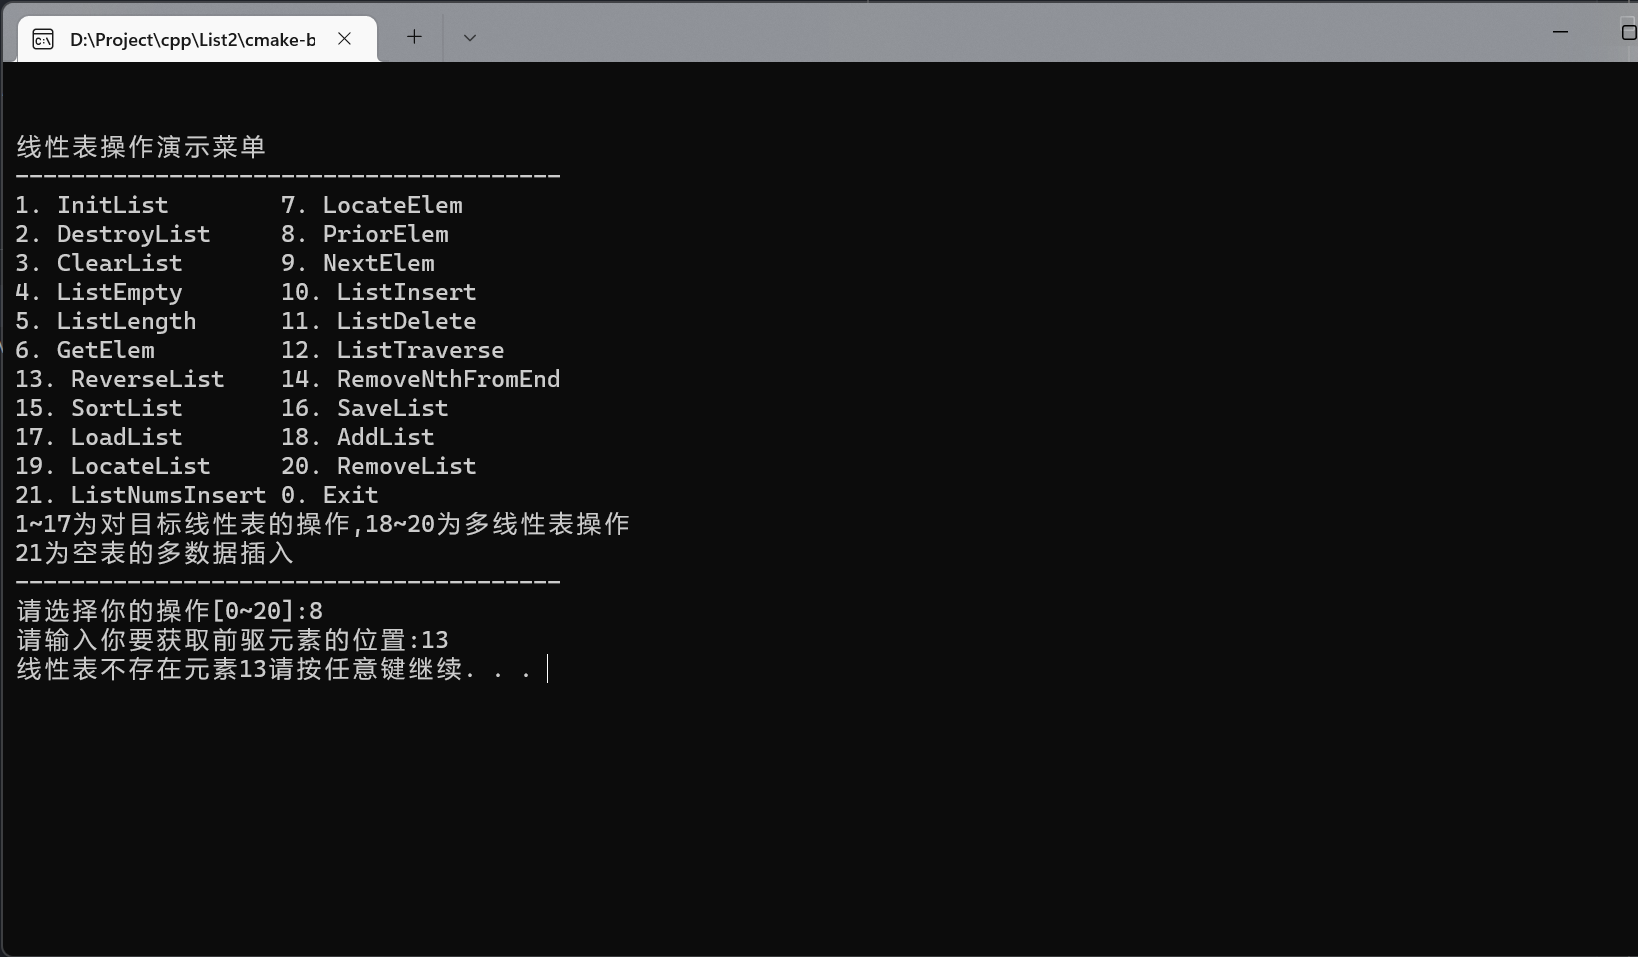
\includegraphics[width=12cm]{images/p1-11.png}}\\
		      \caption{元素测试}
	      \end{figure}
	      \newpage
	\item NextElem测试
	      \begin{table}[htb]
		      \begin{center}
			      \setlength{\tabcolsep}{2.0mm}
			      \caption{Next测试用例表}
			      \label{table8}
			      \begin{tabular}{|c|c|c|c|}
				      \hline
				      测试用例   & 输入               & 理论结果              & 测试结果              \\
				      \hline
				      \hline
				      List       & 界面选9,输入位置-2 & 元素-2的后继元素为3   & 元素-2的后继元素为:3  \\
				      \hline
				      List       & 界面选8,输入位置0  & 不存在元素0的后继元素 & 不存在元素0的后继元素 \\
				      \hline
				      List       & 界面选8,输入位置13 & 线性表不存在元素13    & 线性表不存在元素13    \\
				      \hline
				      未初始化表 & 界面选8            & 线性表不存在          & 线性表不存在          \\
				      \hline
			      \end{tabular}
		      \end{center}
	      \end{table}
	      \begin{figure}[htb]
		      \centering
		      \subfloat[正确元素测试图]{\label{fig1-11}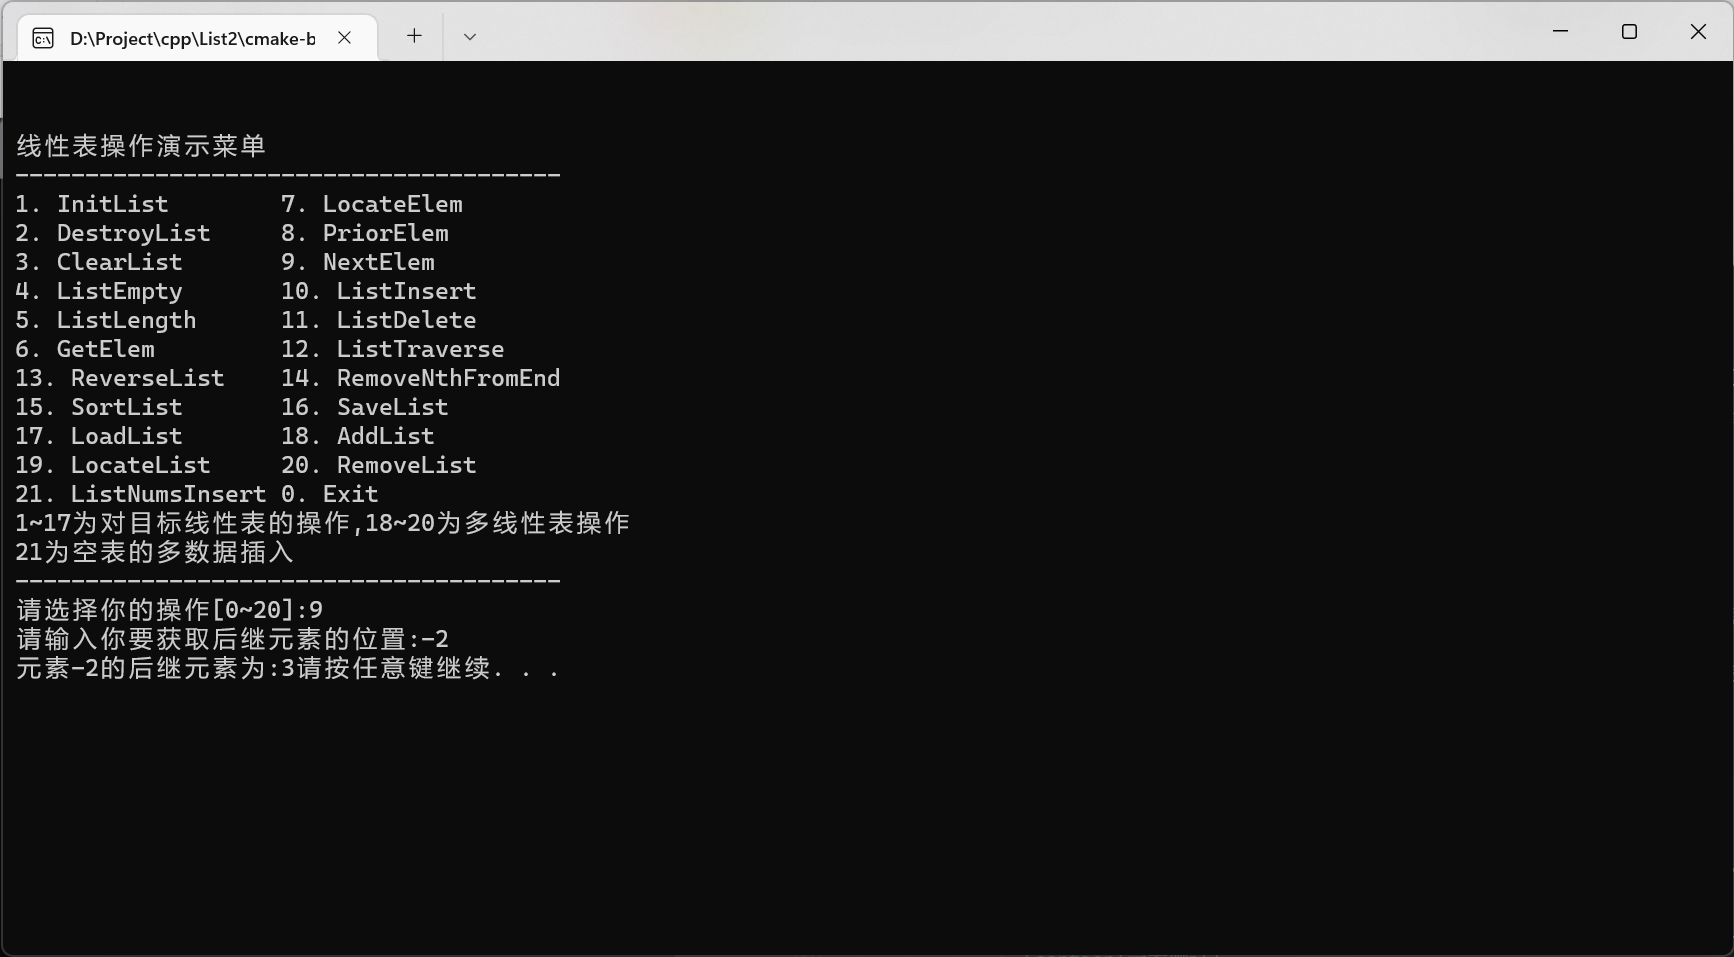
\includegraphics[width=7cm]{images/p1-12.png}}\quad
		      \subfloat[首位置元素测试图]{\label{fig1-12}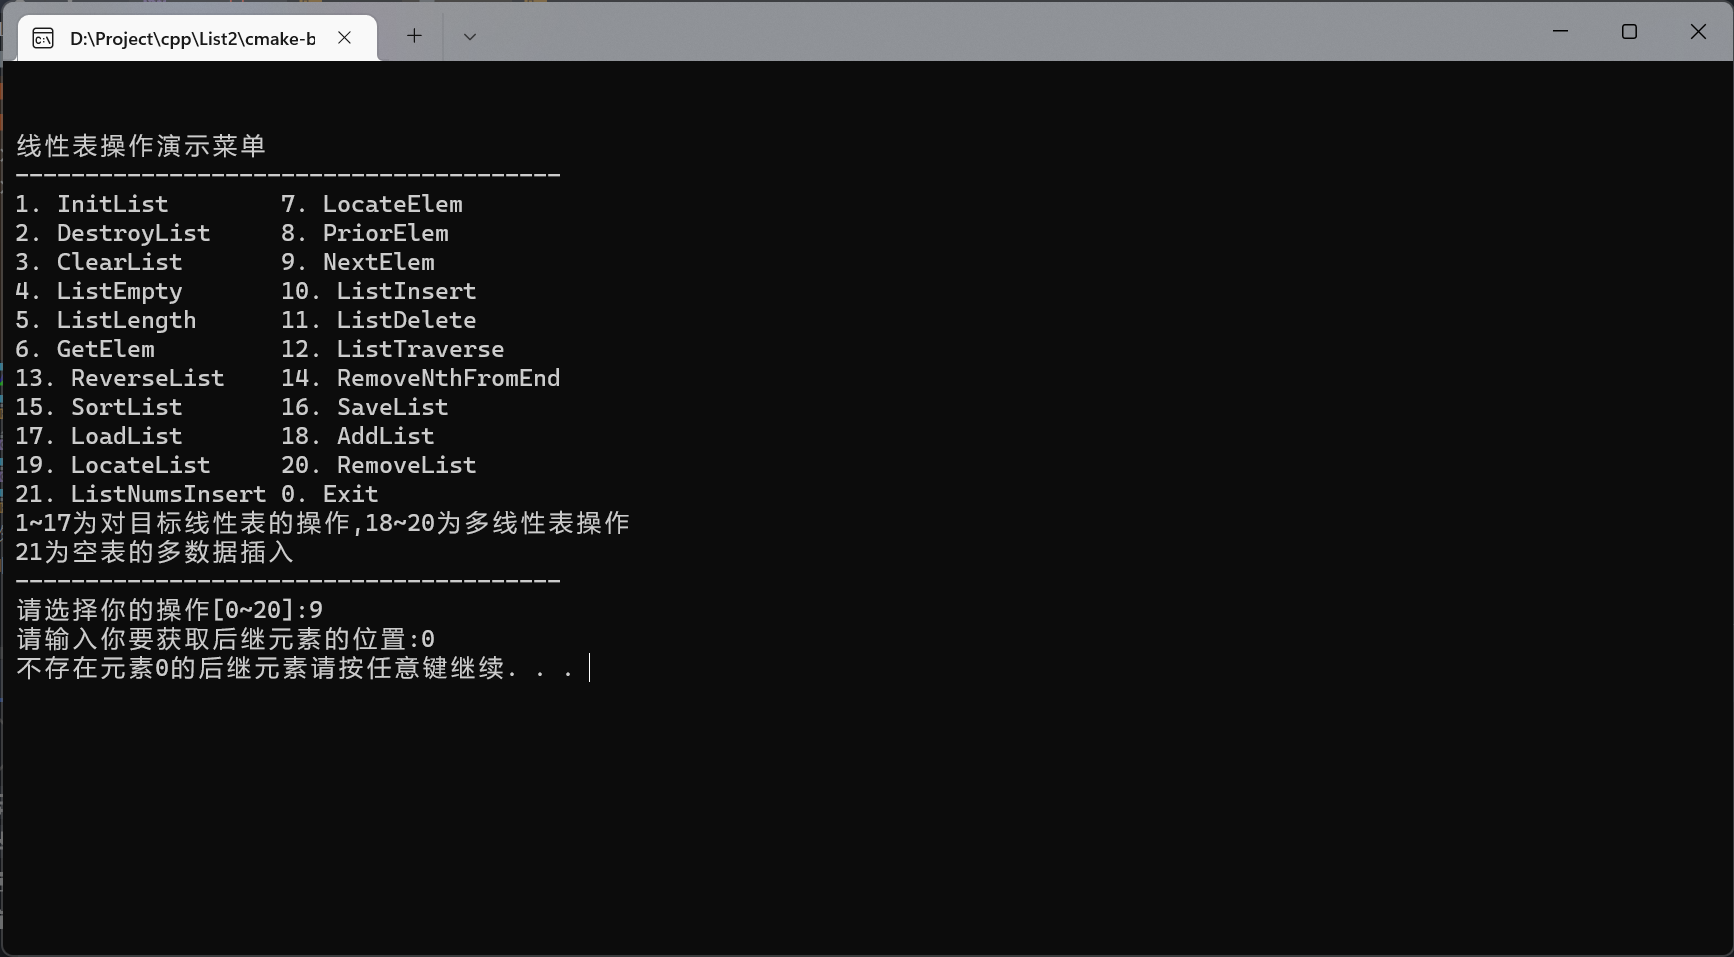
\includegraphics[width=7cm]{images/p1-13.png}}\quad
		      \subfloat[错误元素测试图]{\label{fig1-13}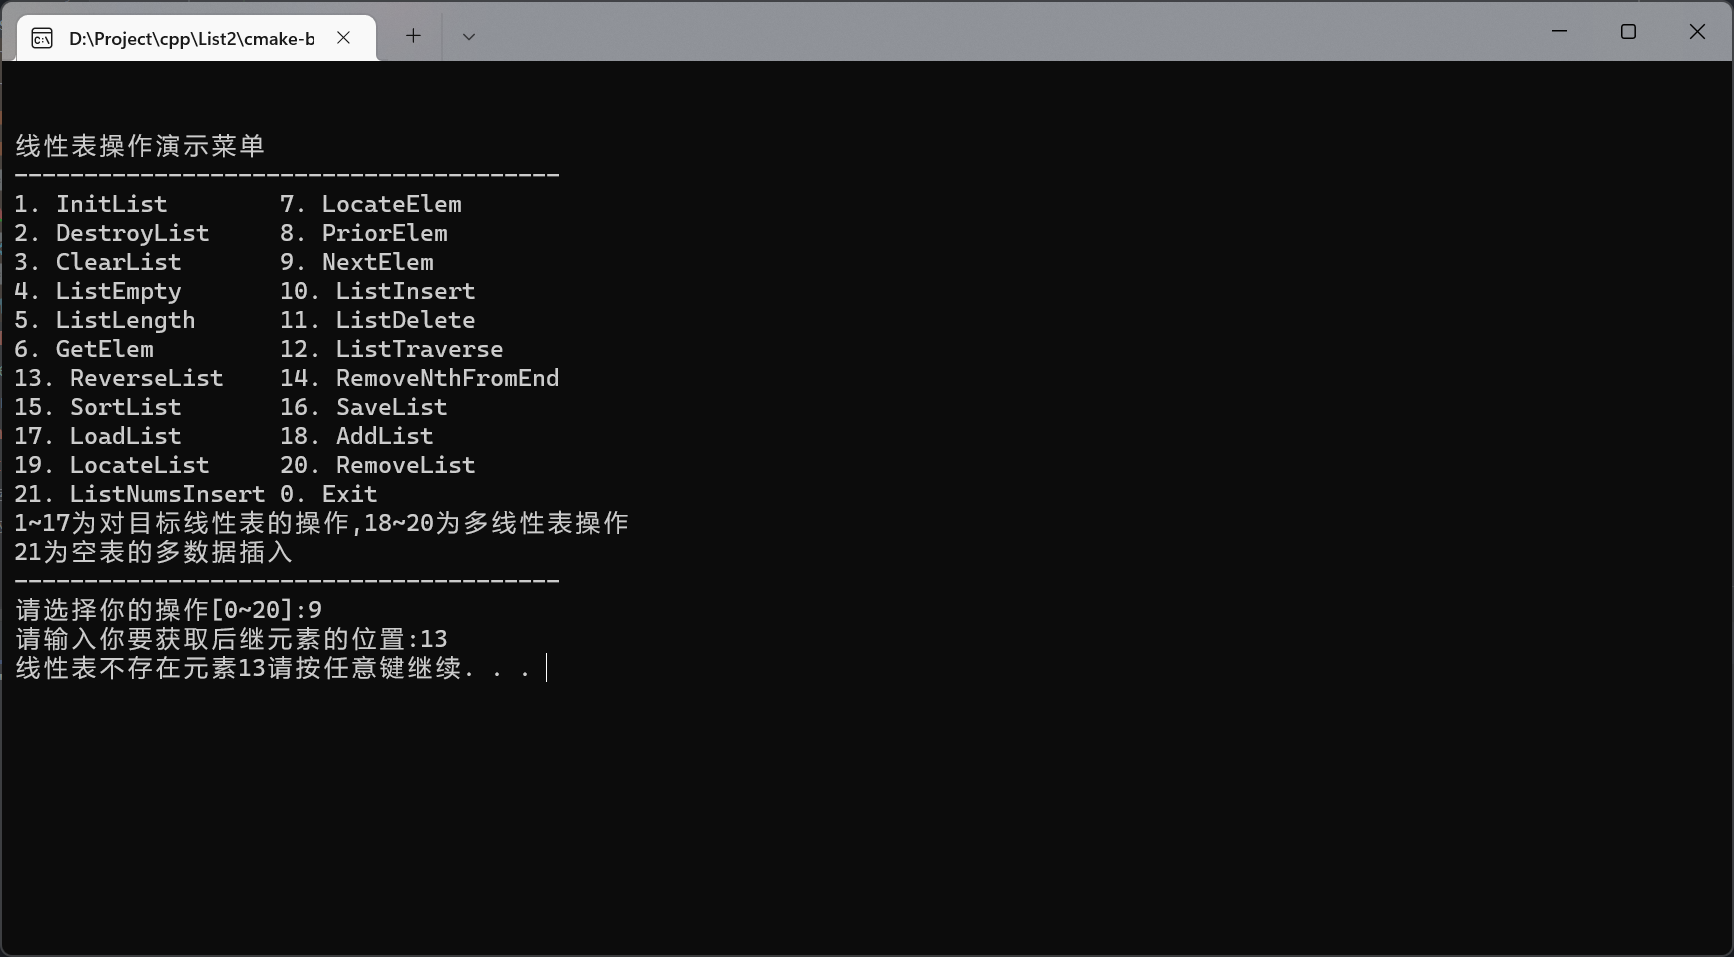
\includegraphics[width=12cm]{images/p1-14.png}}\\
		      \caption{元素测试}
	      \end{figure}
	      \newpage
	\item ListInsert测试
	      \begin{table}[htb]
		      \begin{center}
			      \setlength{\tabcolsep}{2.0mm}
			      \caption{ListInsert测试用例表}
			      \label{table9}
			      \begin{tabular}{|c|c|c|c|}
				      \hline
				      测试用例   & 输入              & 理论结果     & 测试结果     \\
				      \hline
				      \hline
				      List       & 界面选10 输入6 12 & 插入成功     & 插入成功     \\
				      \hline
				      List       & 界面选10,输入13 4 & 插入失败     & 插入失败     \\
				      \hline
				      未初始化表 & 界面选10          & 线性表不存在 & 线性表不存在 \\
				      \hline
			      \end{tabular}
		      \end{center}
	      \end{table}
	      \begin{figure}[htb]
		      \centering
		      \subfloat[正确位置测试图]{\label{fig1-14}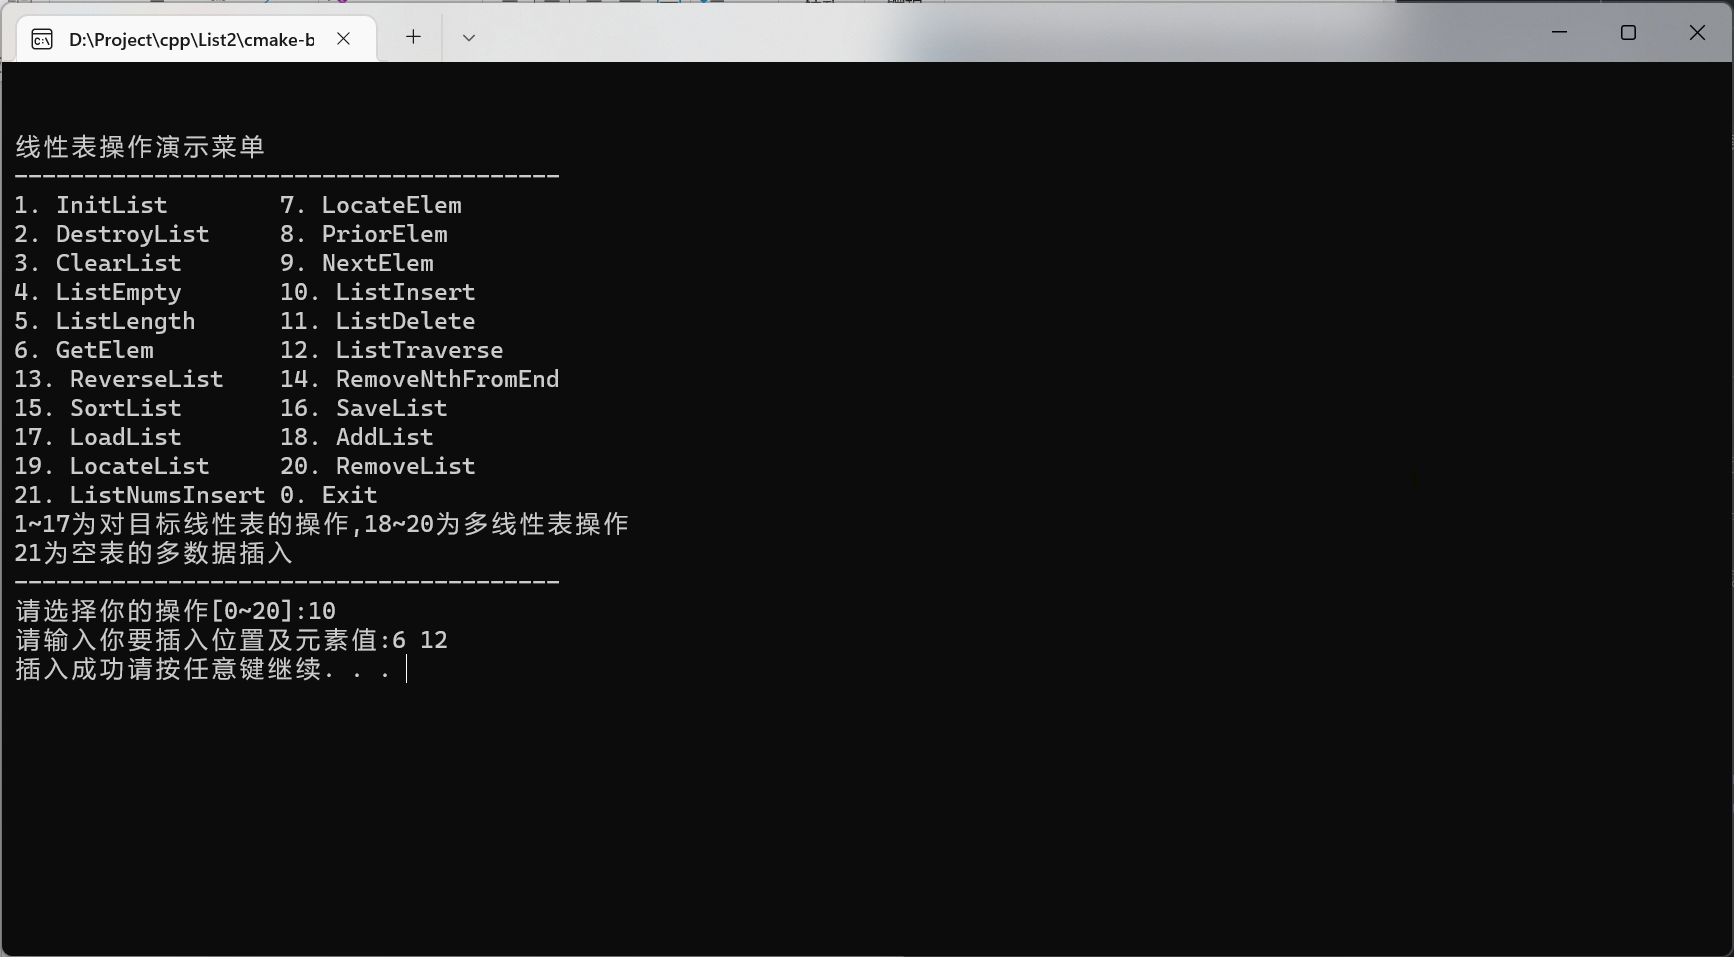
\includegraphics[width=12cm]{images/p1-15.png}}\quad
		      \subfloat[错误位置测试图]{\label{fig1-15}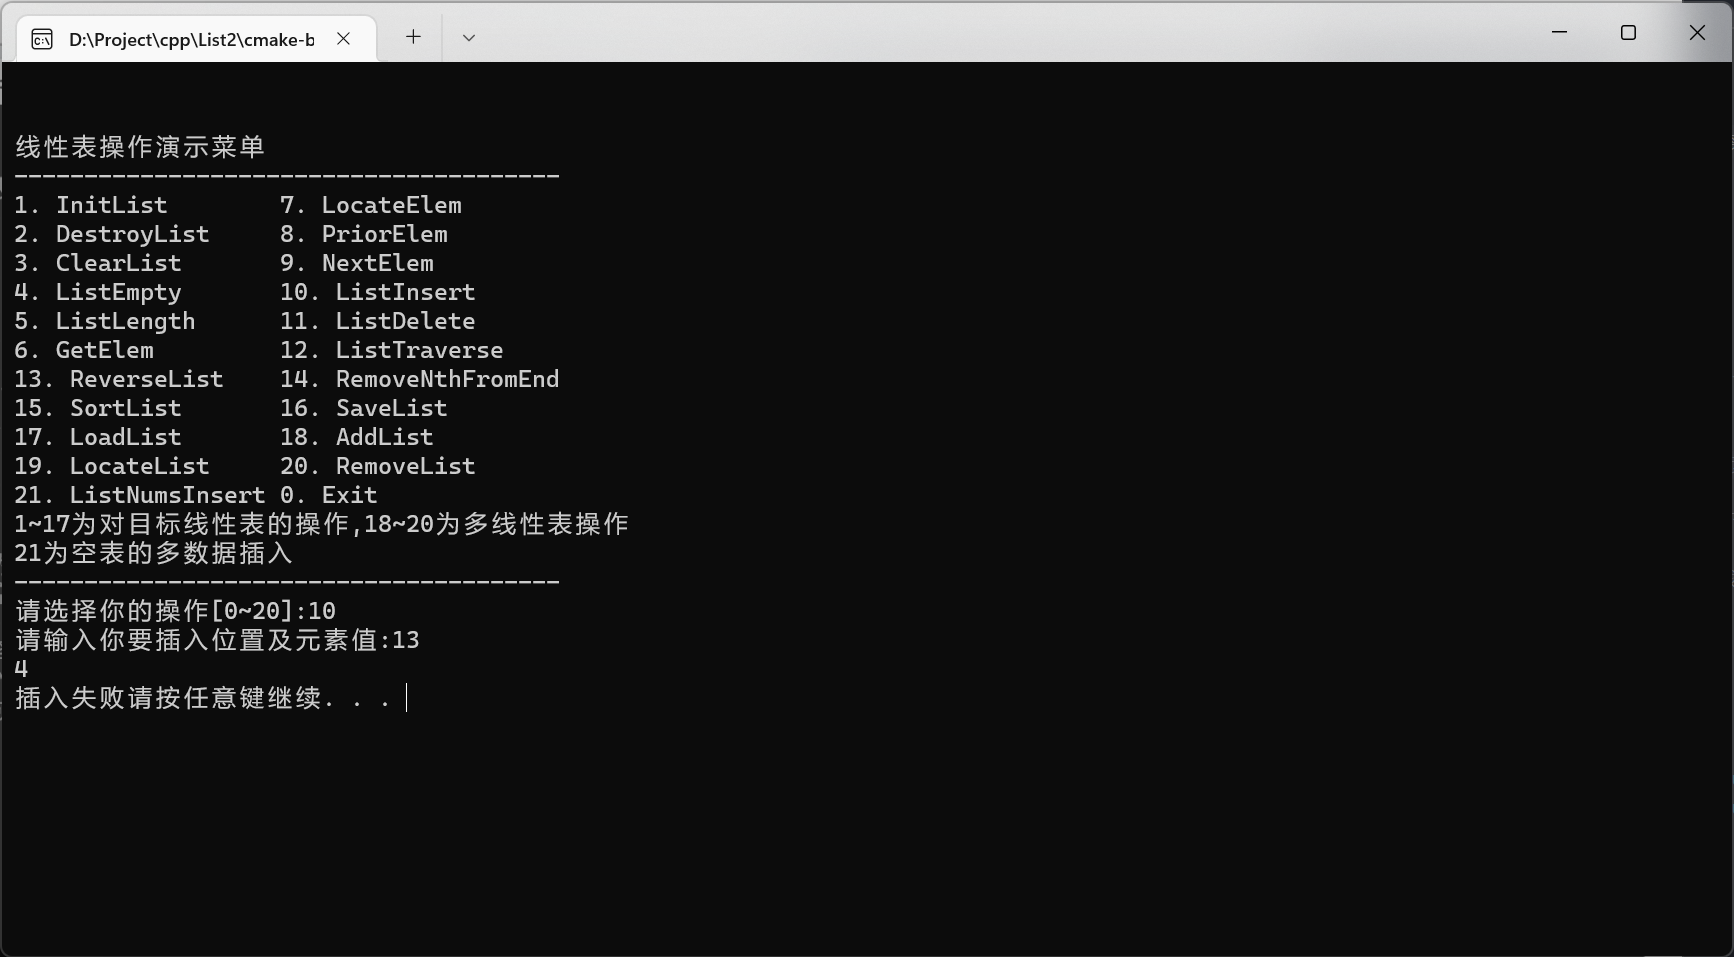
\includegraphics[width=12cm]{images/p1-16.png}}\\
		      \caption{元素测试}
	      \end{figure}
	      \newpage
	\item ListDelete测试
	      \begin{table}[htb]
		      \begin{center}
			      \setlength{\tabcolsep}{2.0mm}
			      \caption{ListDelete测试用例表}
			      \label{table10}
			      \begin{tabular}{|c|c|c|c|}
				      \hline
				      测试用例   & 输入           & 理论结果             & 测试结果             \\
				      \hline
				      \hline
				      List       & 界面选11 输入1 & 删除成功,该元素值为1 & 删除成功,该元素值为1 \\
				      \hline
				      List       & 界面选11,输入9 & 删除失败             & 删除失败             \\
				      \hline
				      未初始化表 & 界面选11       & 线性表不存在         & 线性表不存在         \\
				      \hline
			      \end{tabular}
		      \end{center}
	      \end{table}
	      \begin{figure}[htb]
		      \centering
		      \subfloat[正确位置测试图]{\label{fig1-16}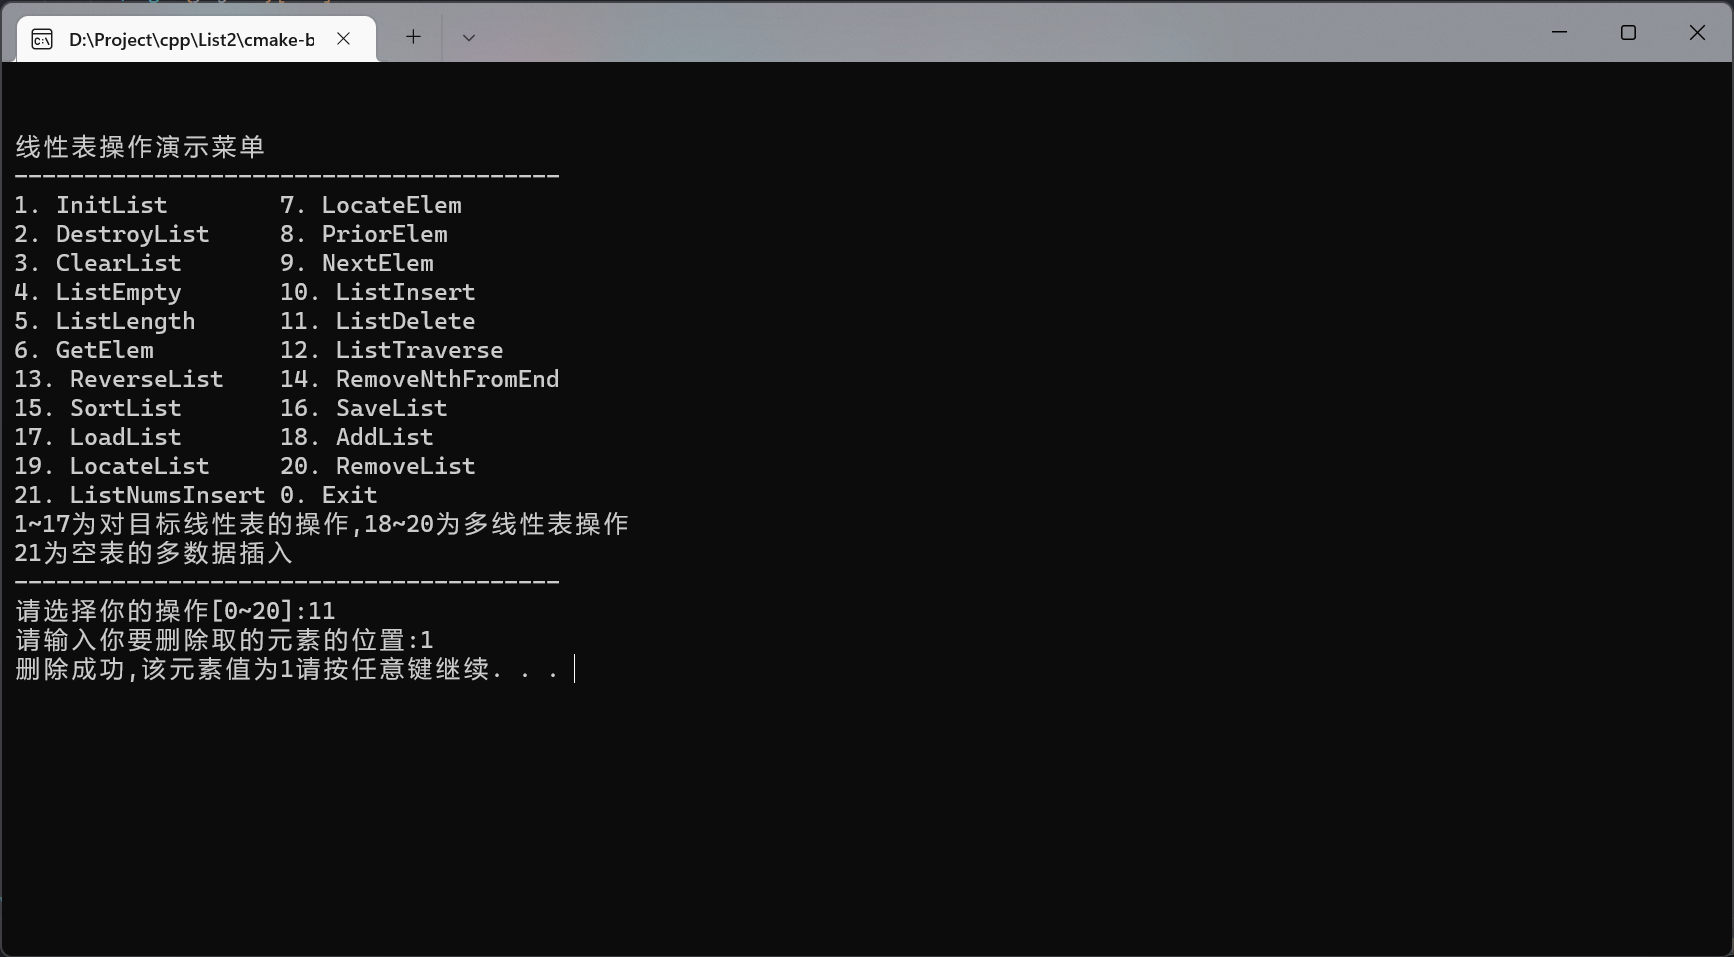
\includegraphics[width=12cm]{images/p1-17.png}}\quad
		      \subfloat[错误位置测试图]{\label{fig1-17}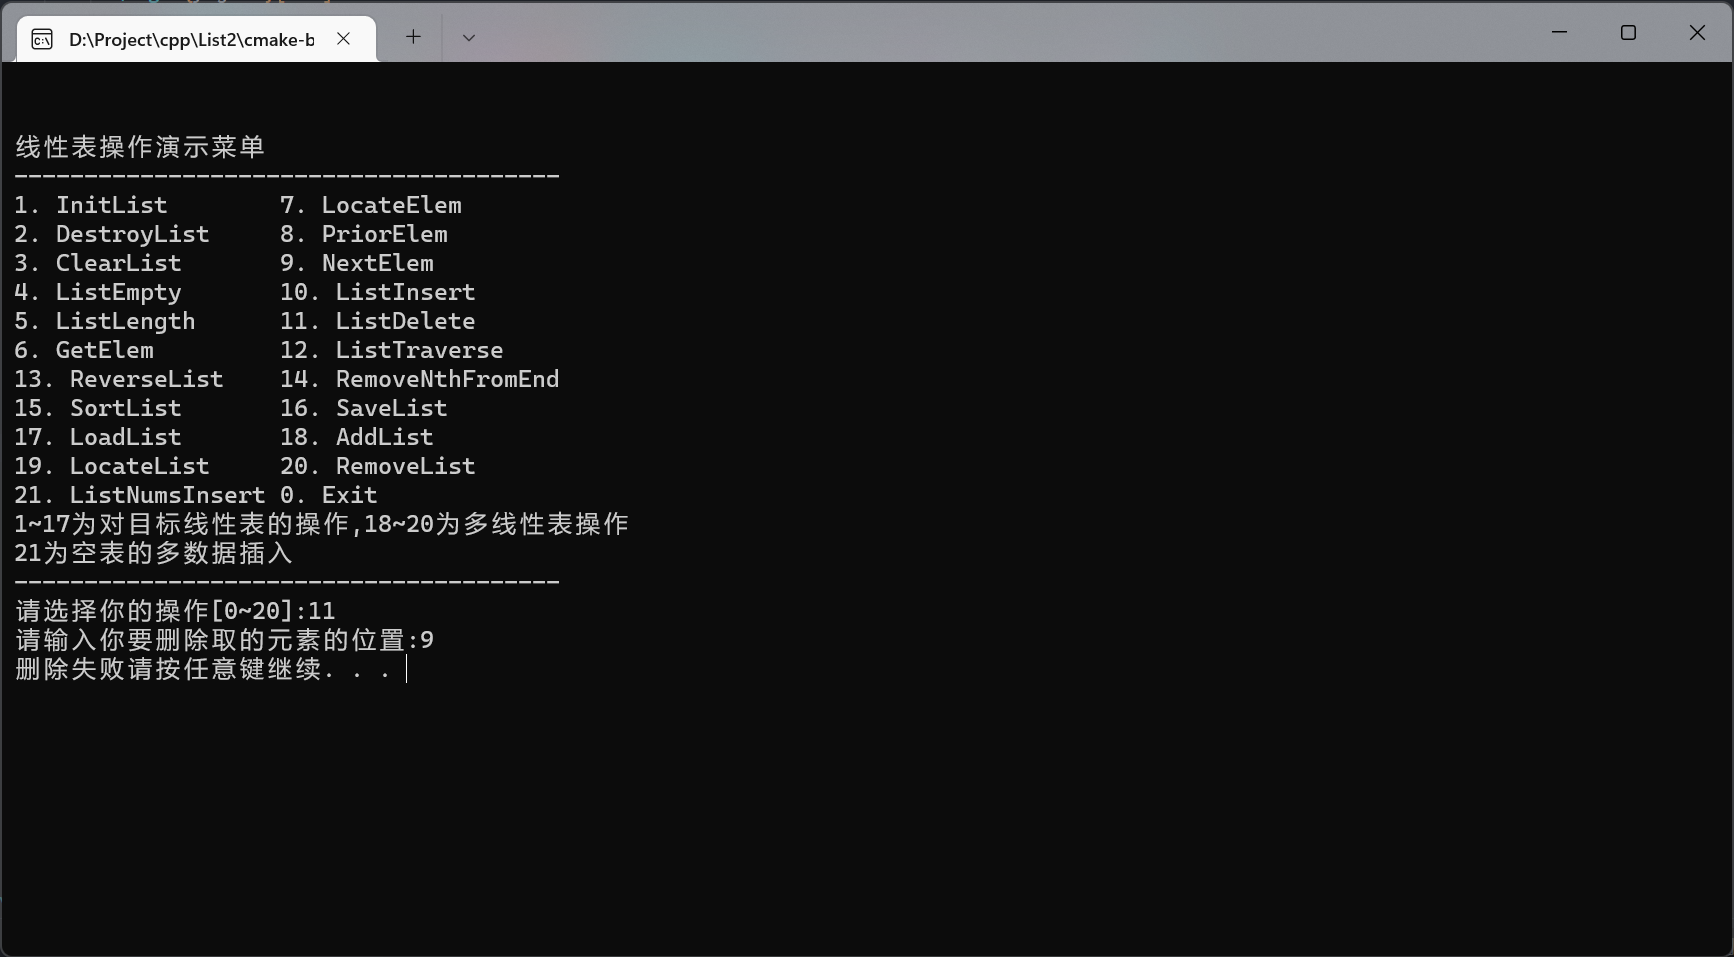
\includegraphics[width=12cm]{images/p1-18.png}}\\
		      \caption{元素测试}
	      \end{figure}
	      \newpage
	\item ListTrabverse测试
	      \begin{table}[htb]
		      \begin{center}
			      \setlength{\tabcolsep}{2.0mm}
			      \caption{ListTrabverse测试用例表}
			      \label{table11}
			      \begin{tabular}{|c|c|c|c|}
				      \hline
				      测试用例   & 输入     & 理论结果     & 测试结果     \\
				      \hline
				      \hline
				      List       & 界面选12 & 1 4 -2 3 0   & 1 4 -2 3 0   \\
				      \hline
				      未初始化表 & 界面选12 & 线性表不存在 & 线性表不存在 \\
				      \hline
			      \end{tabular}
		      \end{center}
	      \end{table}
	      \begin{figure}[htb]
		      \centering
		      \subfloat[测试用例测试图]{\label{fig1-18}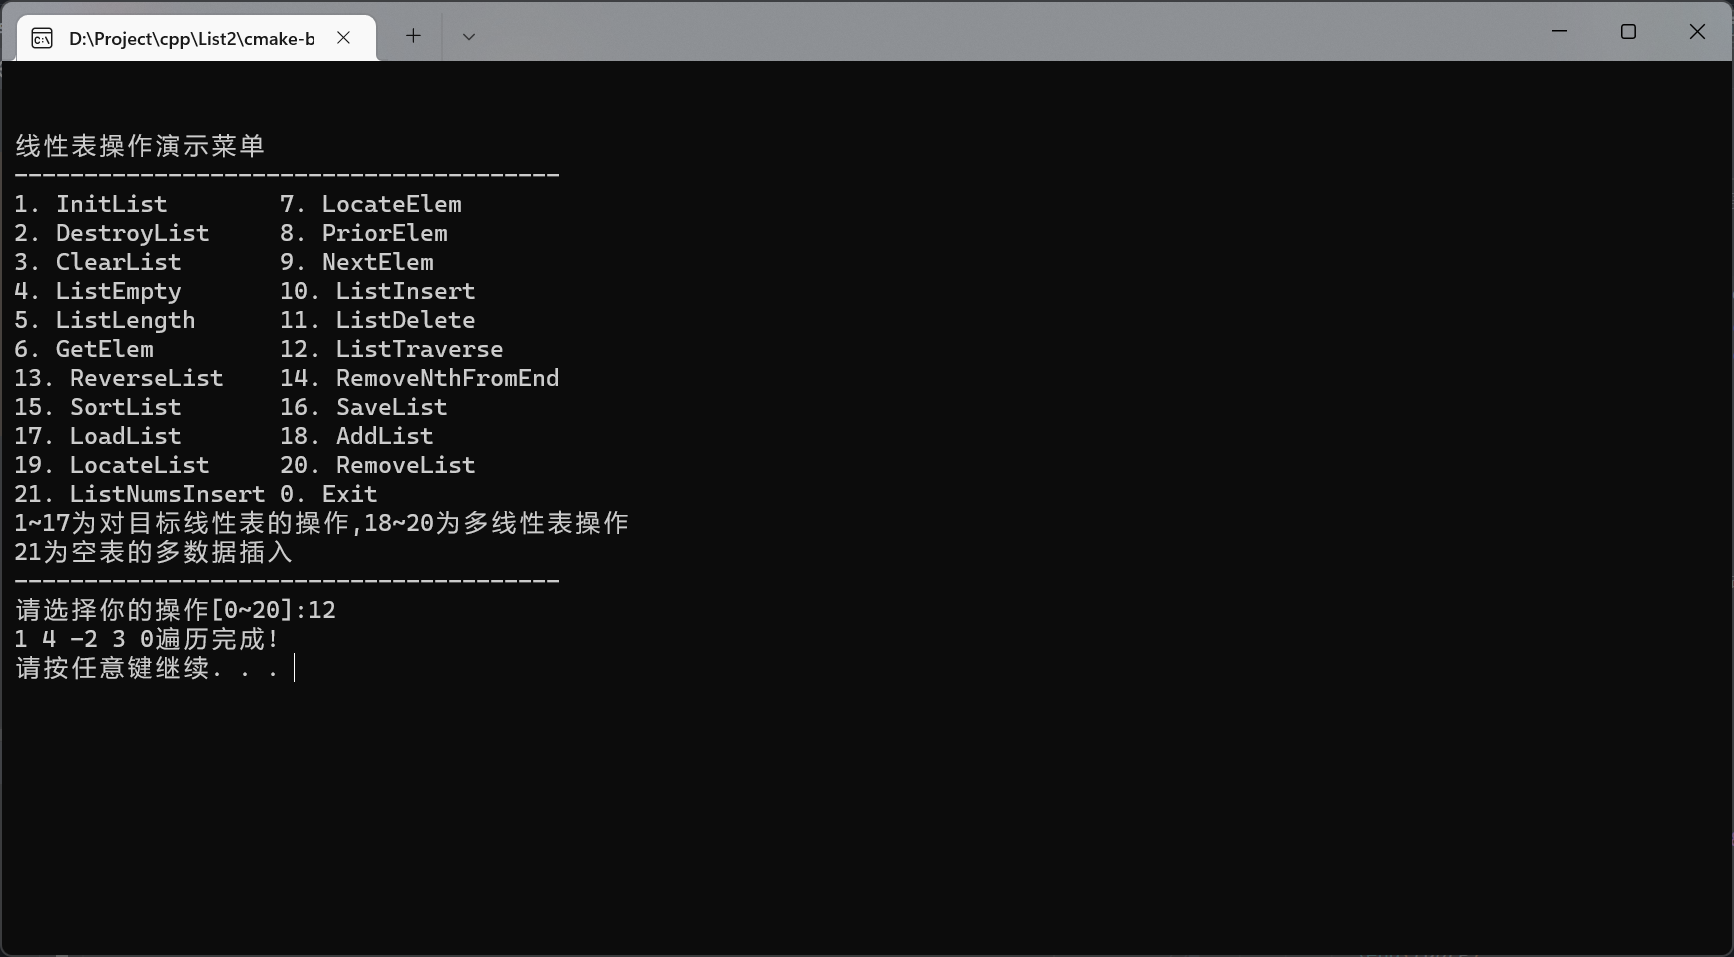
\includegraphics[width=12cm]{images/p1-19.png}}\quad
		      \subfloat[线性表不存在测试图]{\label{fig1-19}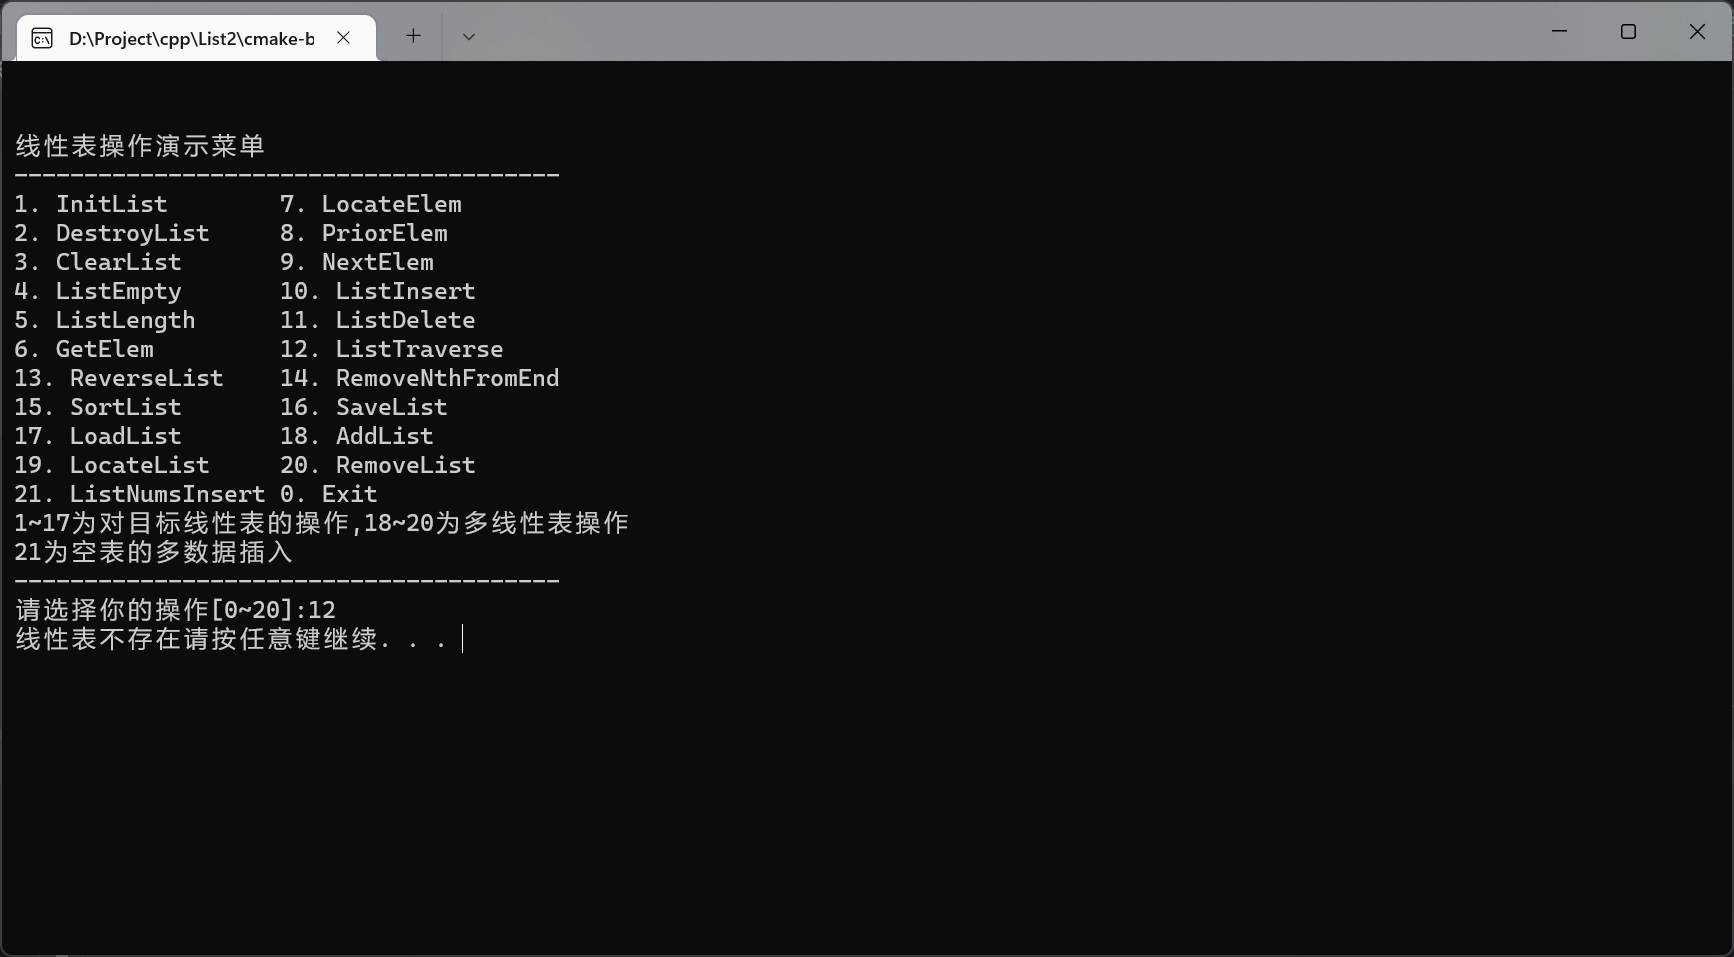
\includegraphics[width=12cm]{images/p1-20.png}}\\
		      \caption{遍历链表测试}
	      \end{figure}
	      \newpage
	\item ReverseList测试
	      \begin{table}[htb]
		      \begin{center}
			      \setlength{\tabcolsep}{2.0mm}
			      \caption{ReverseList测试用例表}
			      \label{table16}
			      \begin{tabular}{|c|c|c|c|}
				      \hline
				      测试用例   & 输入     & 理论结果                               & 测试结果     \\
				      \hline
				      \hline
				      List       & 界面选13 & 线性表已翻转                0 3 -2 4 1 & 线性表已翻转 \\
				      \hline
				      未初始化表 & 界面选13 & 线性表不存在                           & 线性表不存在 \\
				      \hline
				      NULL       & 界面选13 & 线性表为空                             & 线性表为空   \\
				      \hline
			      \end{tabular}
		      \end{center}
	      \end{table}
	      \begin{figure}[htb]
		      \centering
		      \subfloat[NULL表测试图]{\label{fig1-27}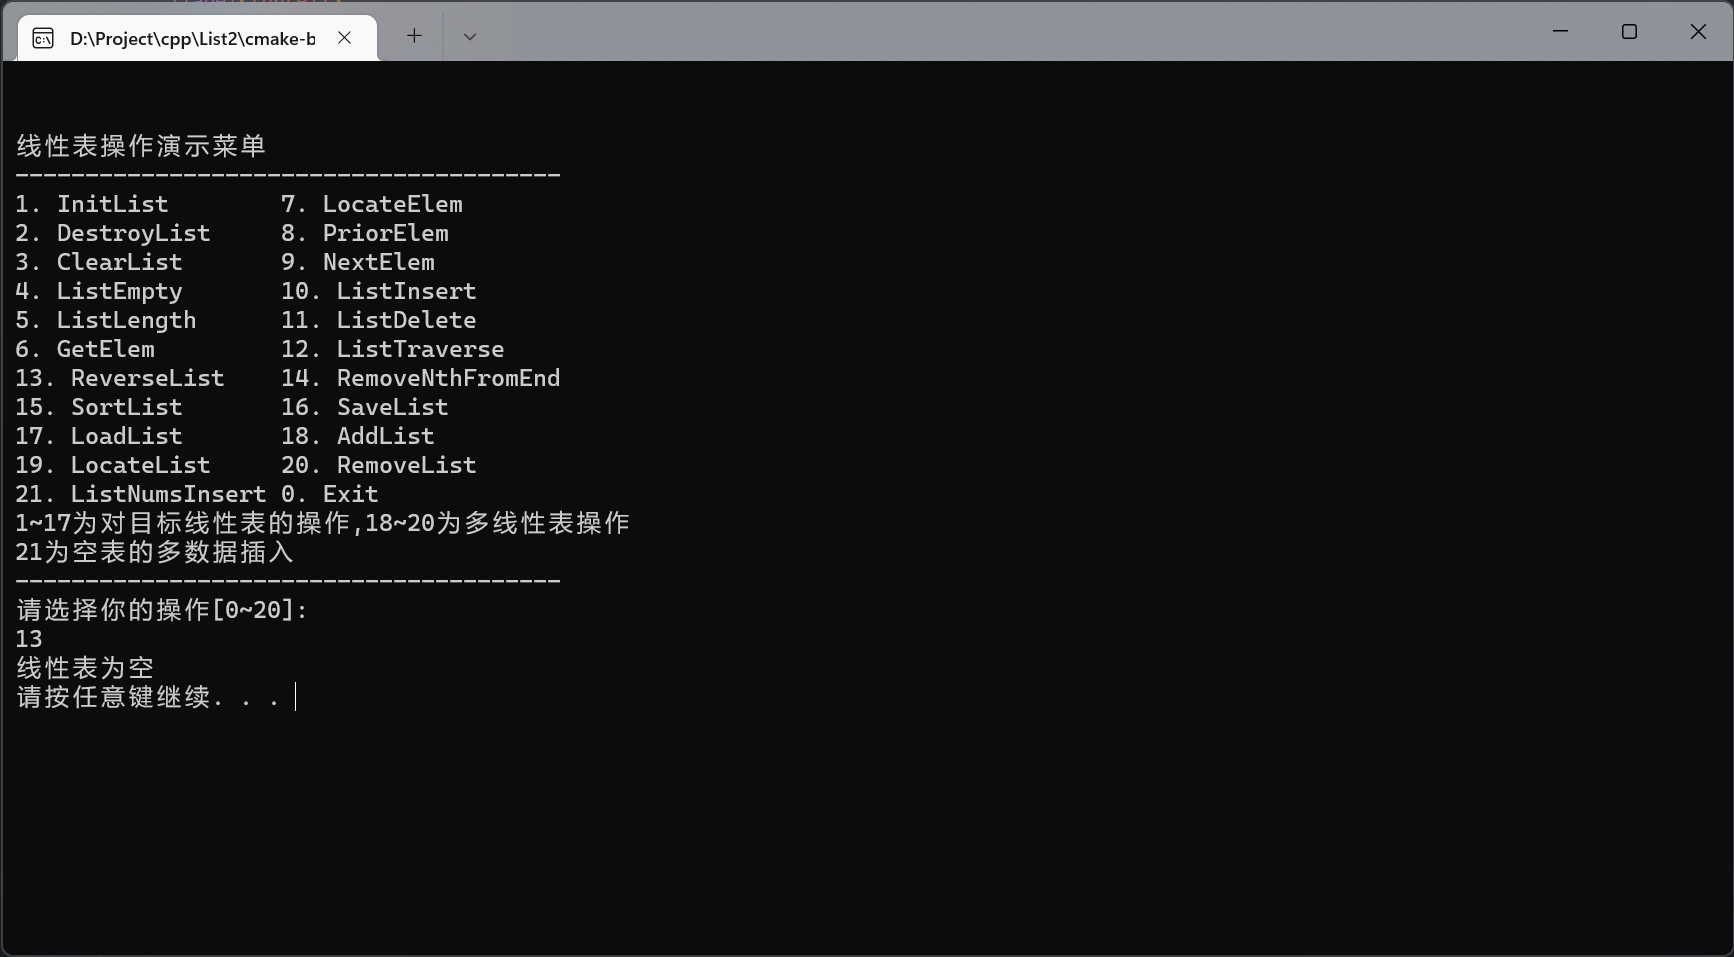
\includegraphics[width=7cm]{images/p1-30.png}}\quad
		      \subfloat[未初始化表测试图]{\label{fig1-28}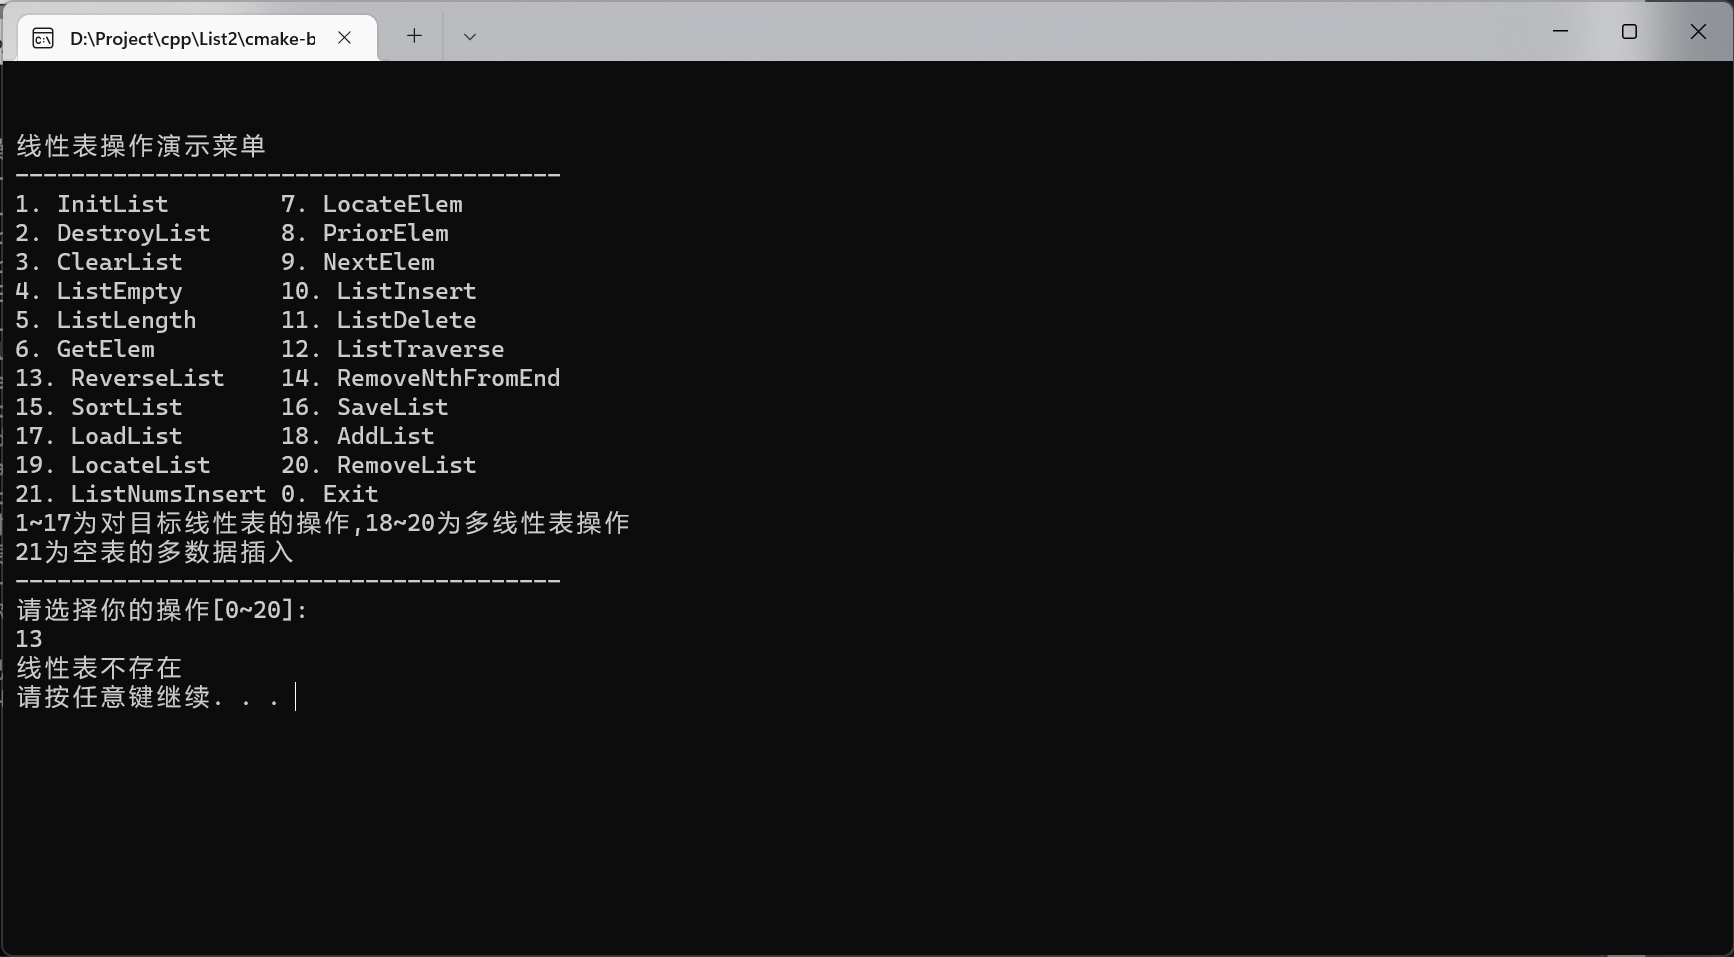
\includegraphics[width=7cm]{images/p1-29.png}}\quad
		      \subfloat[测试用例测试图]{\label{fig1-29}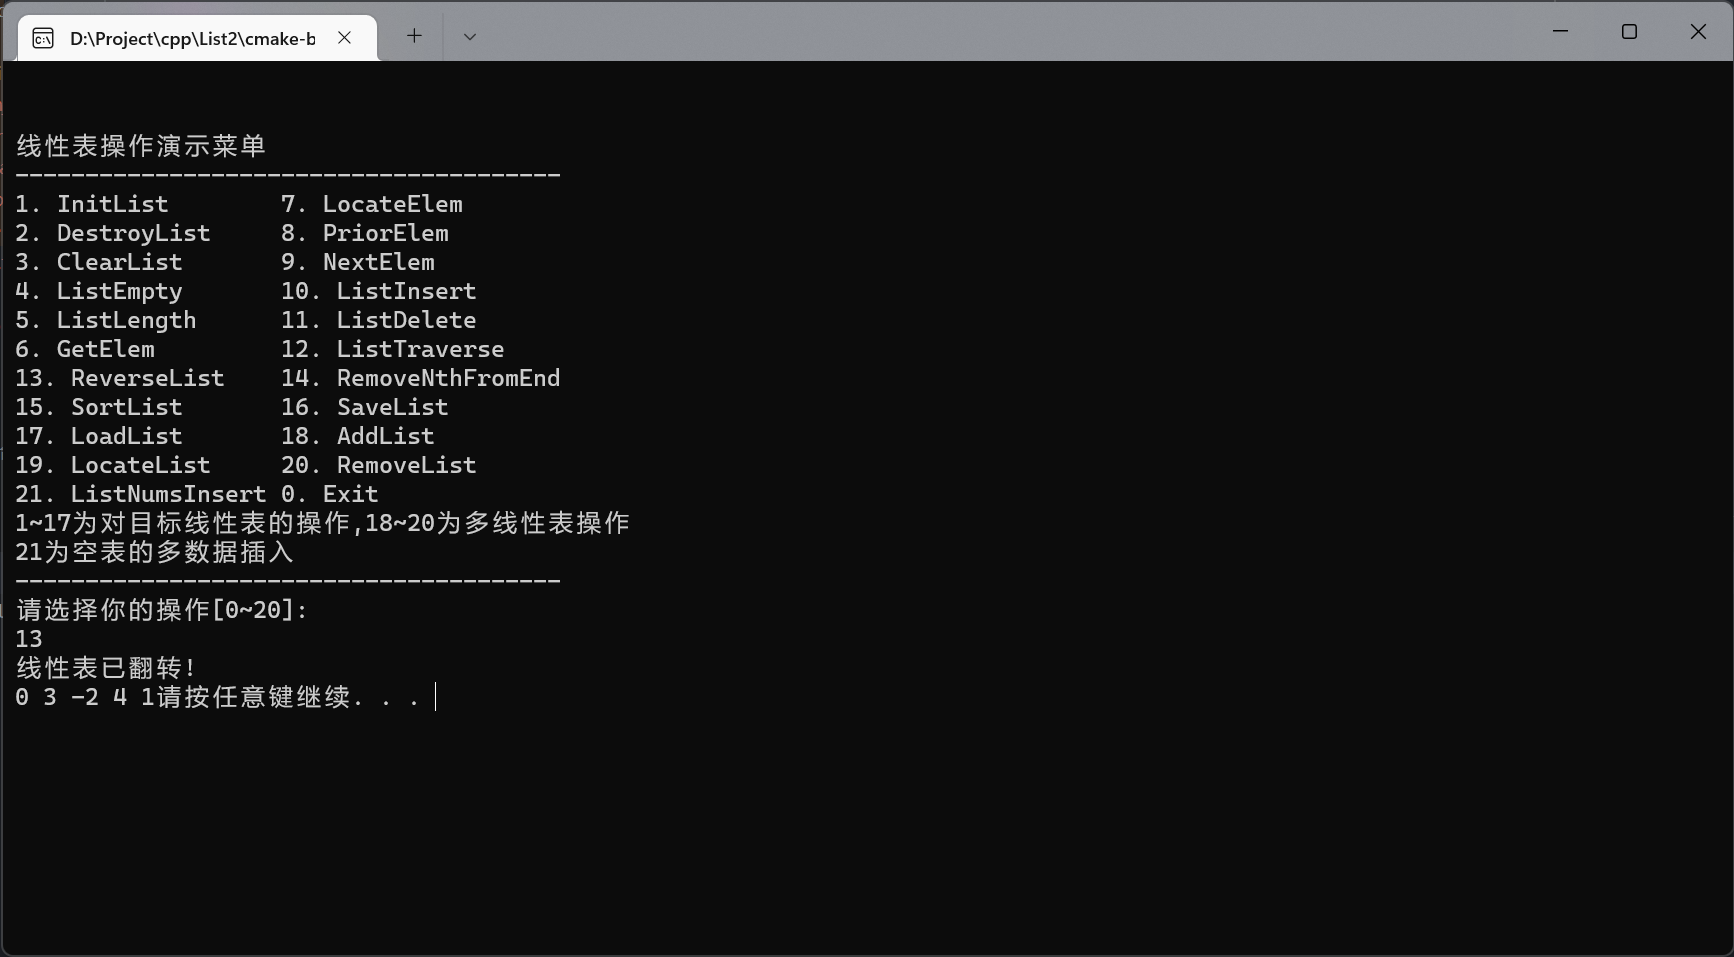
\includegraphics[width=12cm]{images/p1-28.png}}\\
		      \caption{翻转链表测试}
	      \end{figure}
	      \newpage
	\item RemoveNthFromEnd测试
	      \begin{table}[htb]
		      \begin{center}
			      \setlength{\tabcolsep}{2.0mm}
			      \caption{RemoveNthFromEnd测试用例表}
			      \label{table17}
			      \begin{tabular}{|c|c|c|c|}
				      \hline
				      测试用例   & 输入           & 理论结果     & 测试结果     \\
				      \hline
				      \hline
				      List       & 界面选14,输入5 & 删除成功     & 删除成功     \\
				      \hline
				      List       & 界面选14,输入6 & 删除失败     & 删除失败     \\
				      \hline
				      未初始化表 & 界面选14       & 线性表不存在 & 线性表不存在 \\
				      \hline
				      NULL       & 界面选14       & 线性表为空   & 线性表为空   \\
				      \hline
			      \end{tabular}
		      \end{center}
	      \end{table}
	      \begin{figure}[htb]
		      \centering
		      \subfloat[错误位置测试图]{\label{fig1-30}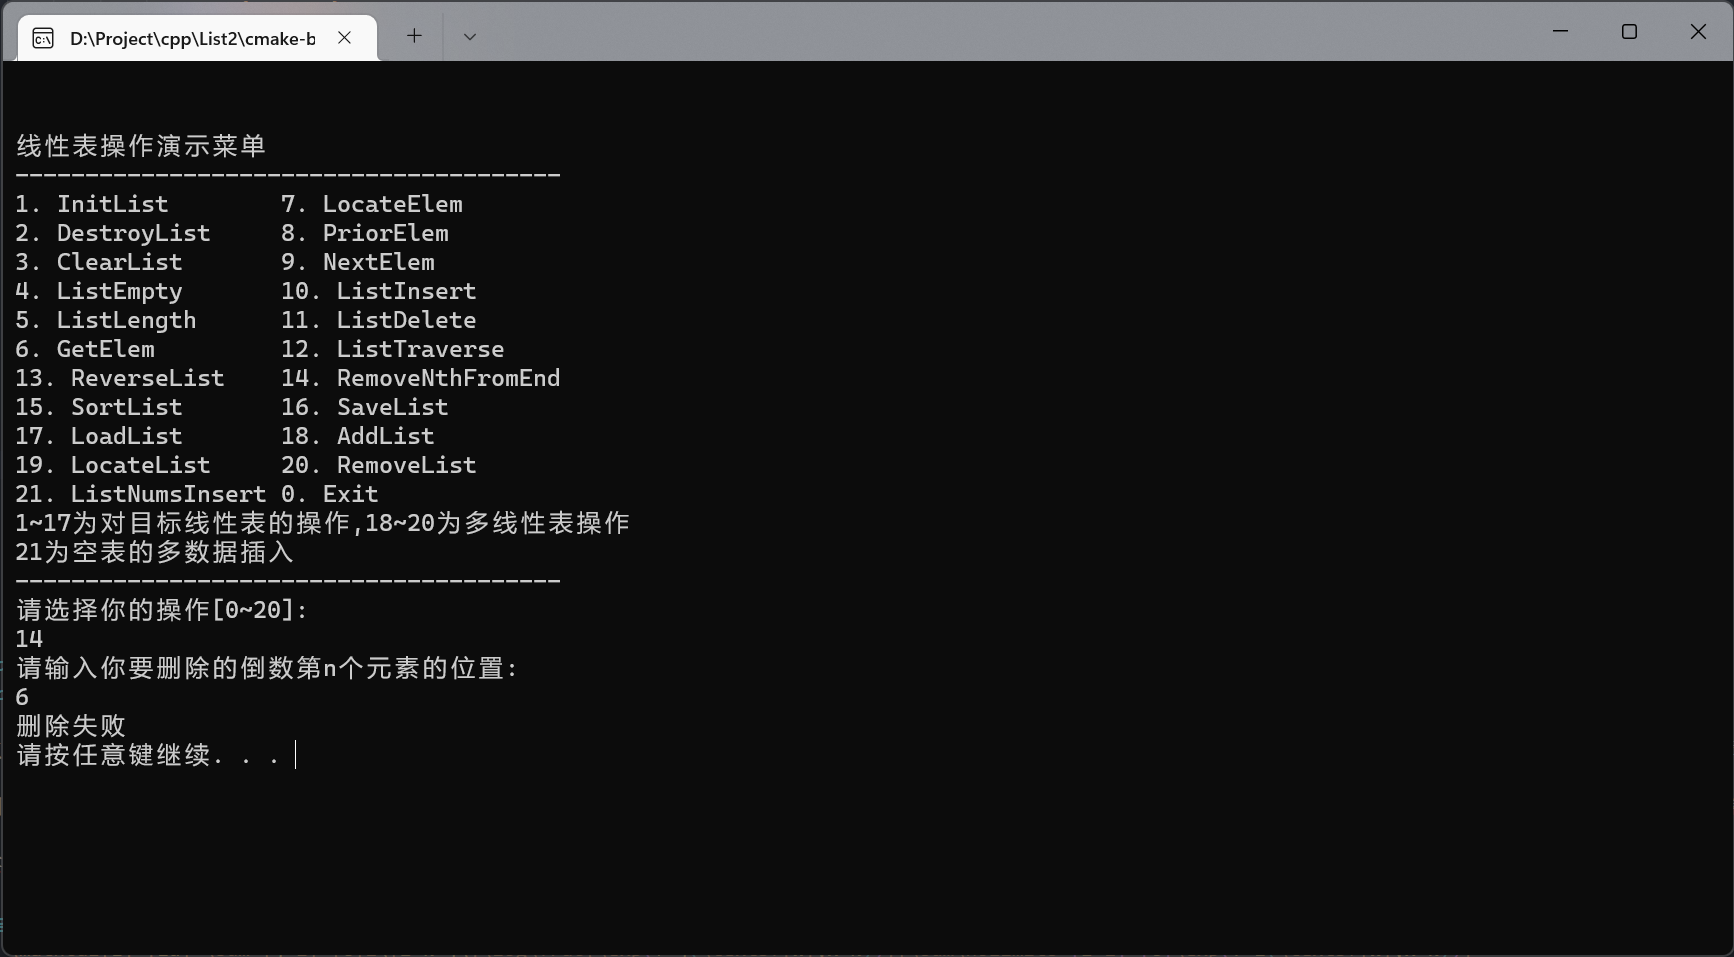
\includegraphics[width=10cm]{images/p1-32.png}}\quad
		      \subfloat[正确位置测试图]{\label{fig1-31}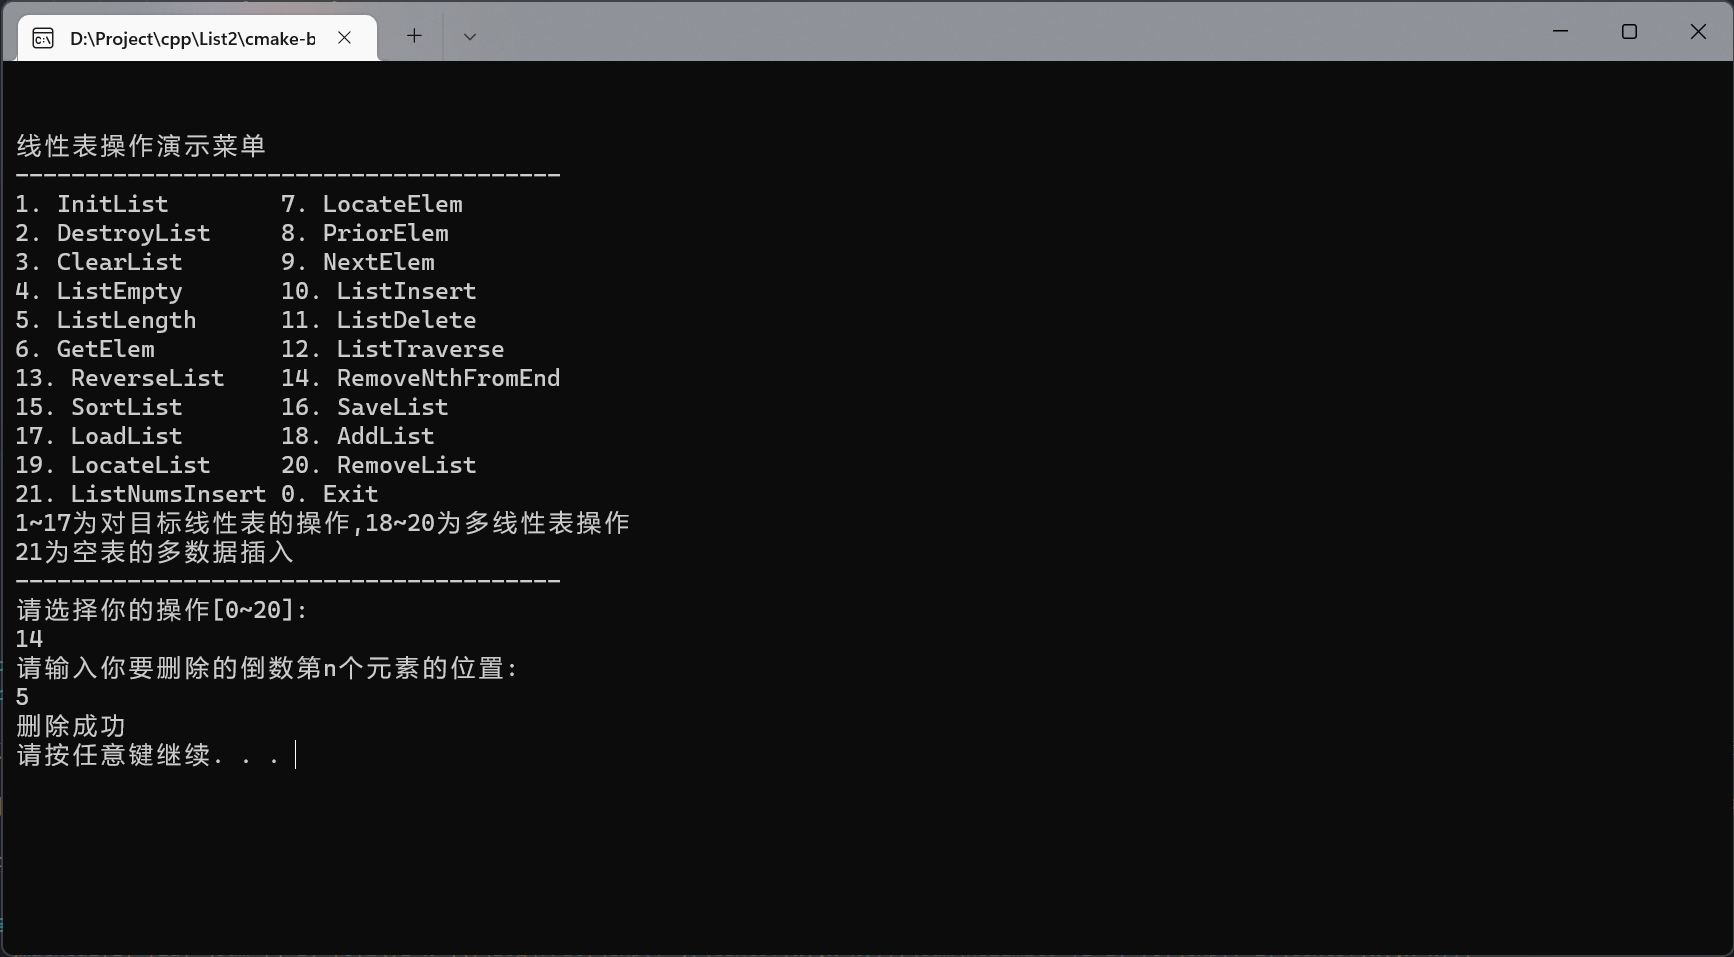
\includegraphics[width=10cm]{images/p1-31.png}}\\
		      \caption{删除倒数第n个测试}
	      \end{figure}
	      \newpage
	\item SortList测试
	      \begin{table}[htb]
		      \begin{center}
			      \setlength{\tabcolsep}{2.0mm}
			      \caption{SortList测试用例表}
			      \label{table18}
			      \begin{tabular}{|c|c|c|c|}
				      \hline
				      测试用例   & 输入     & 理论结果            & 测试结果            \\
				      \hline
				      \hline
				      List       & 界面选15 & 排序成功 -2 0 1 3 4 & 排序成功 -2 0 1 3 4 \\
				      \hline
				      未初始化表 & 界面选15 & 线性表不存在        & 线性表不存在        \\
				      \hline
				      NULL       & 界面选15 & 线性表为空          & 线性表为空          \\
				      \hline
			      \end{tabular}
		      \end{center}
	      \end{table}
	      \begin{figure}[htb]
		      \centering
		      \subfloat[NULL测试图]{\label{fig1-32}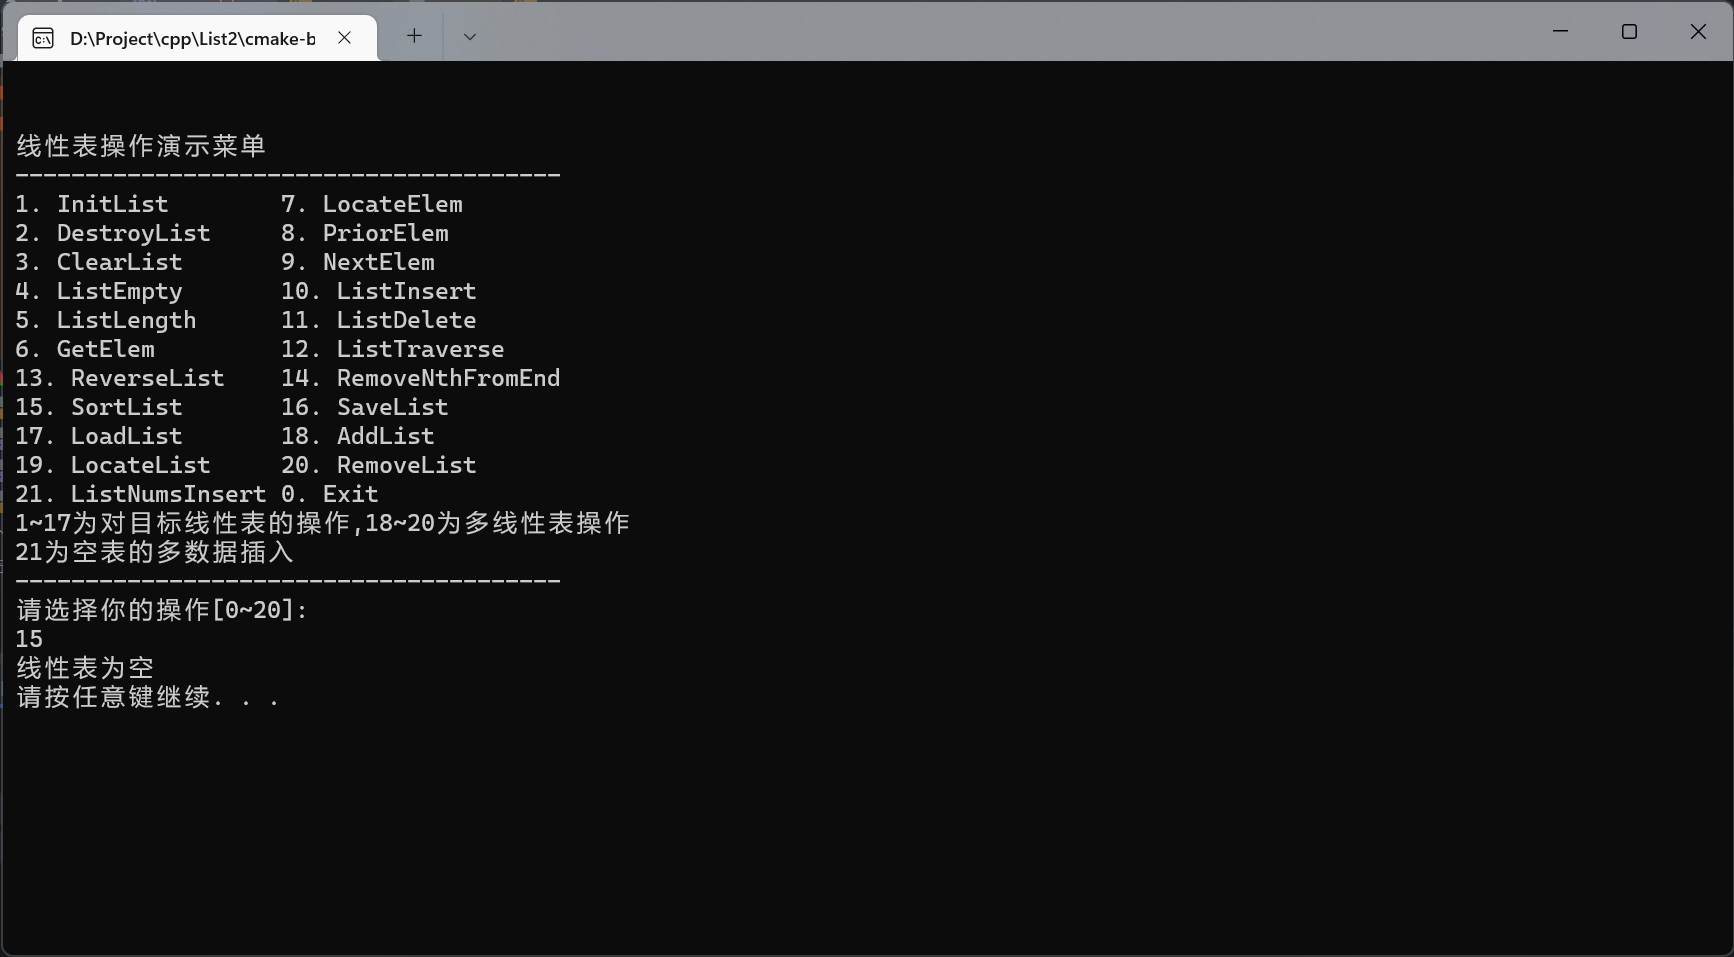
\includegraphics[width=7cm]{images/p1-33.png}}\quad
		      \subfloat[未初始化表测试图]{\label{fig1-33}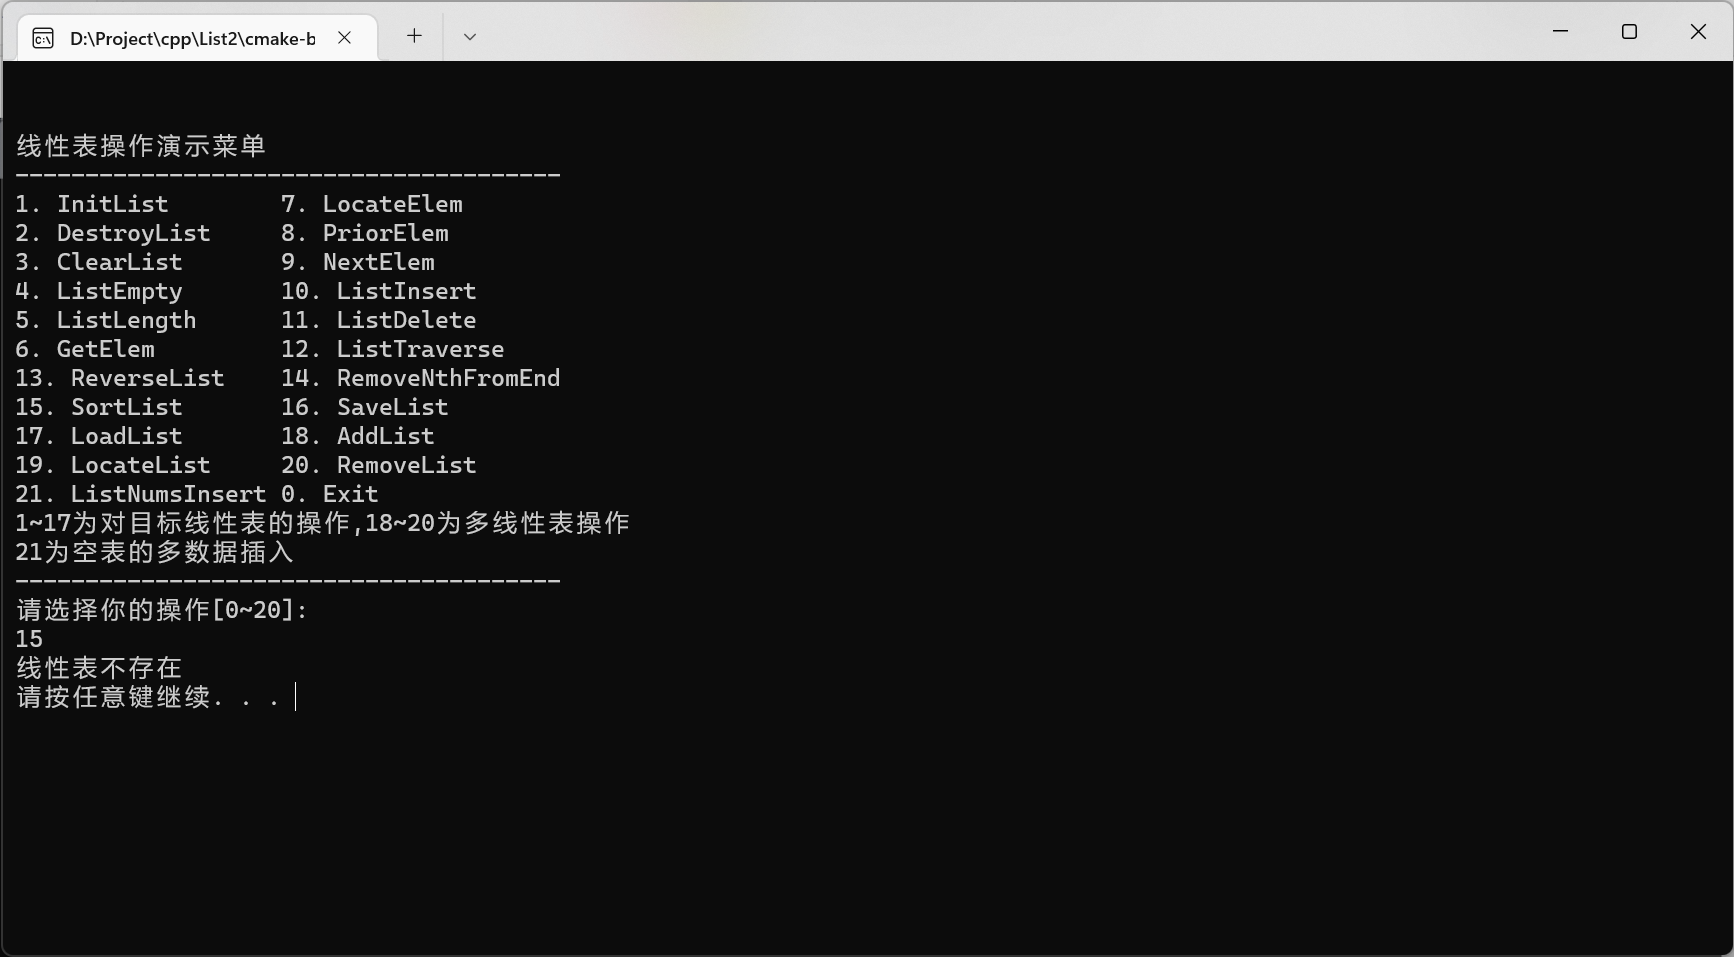
\includegraphics[width=7cm]{images/p1-34.png}}\quad
		      \subfloat[测试用例测试图]{\label{fig1-34}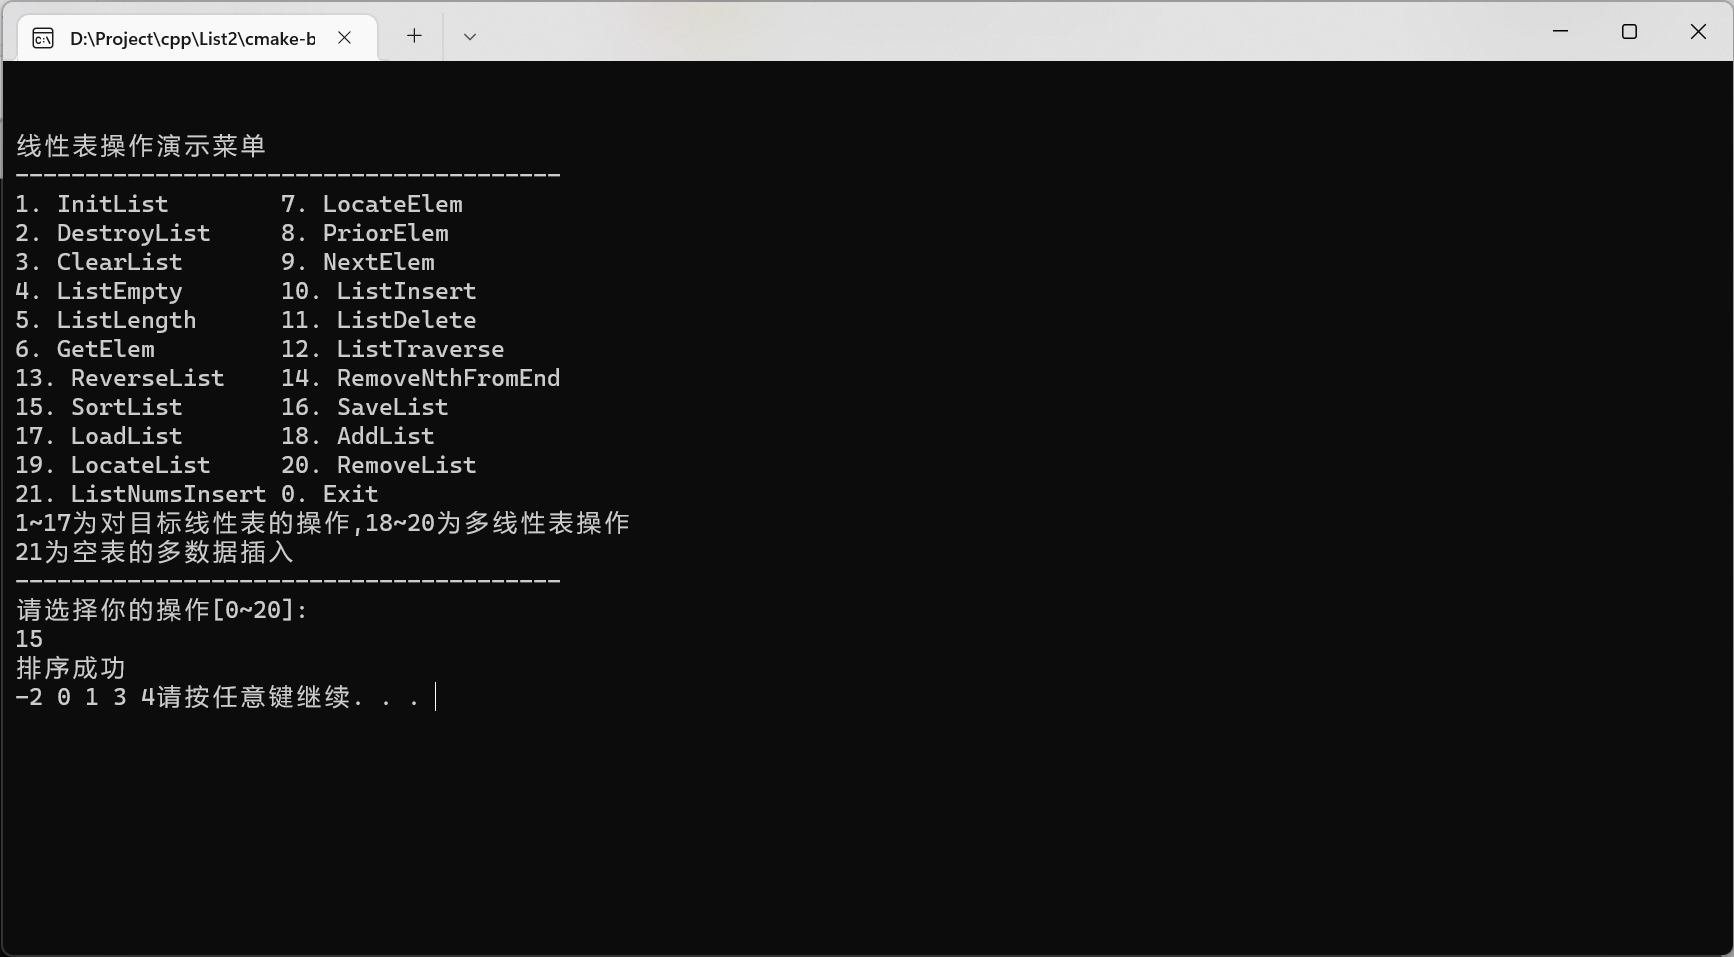
\includegraphics[width=12cm]{images/p1-35.png}}\\
		      \caption{链表排序测试}
	      \end{figure}
	      \newpage
	\item AddList测试
	      \begin{table}[htb]
		      \begin{center}
			      \setlength{\tabcolsep}{2.0mm}
			      \caption{Addlist测试用例表}
			      \label{table19}
			      \begin{tabular}{|c|c|c|c|}
				      \hline
				      测试用例 & 输入                 & 理论结果       & 测试结果       \\
				      \hline
				      \hline
				      表1      & 界面选18,输入表1     & 新建线性表成功 & 新建线性表成功 \\
				      \hline
				      重复表1  & 界面选18,再次输入表1 & 新建线性表失败 & 新建线性表失败 \\
				      \hline
			      \end{tabular}
		      \end{center}
	      \end{table}
	      \begin{figure}[htb]
		      \centering
		      \subfloat[表1测试图]{\label{fig1-35}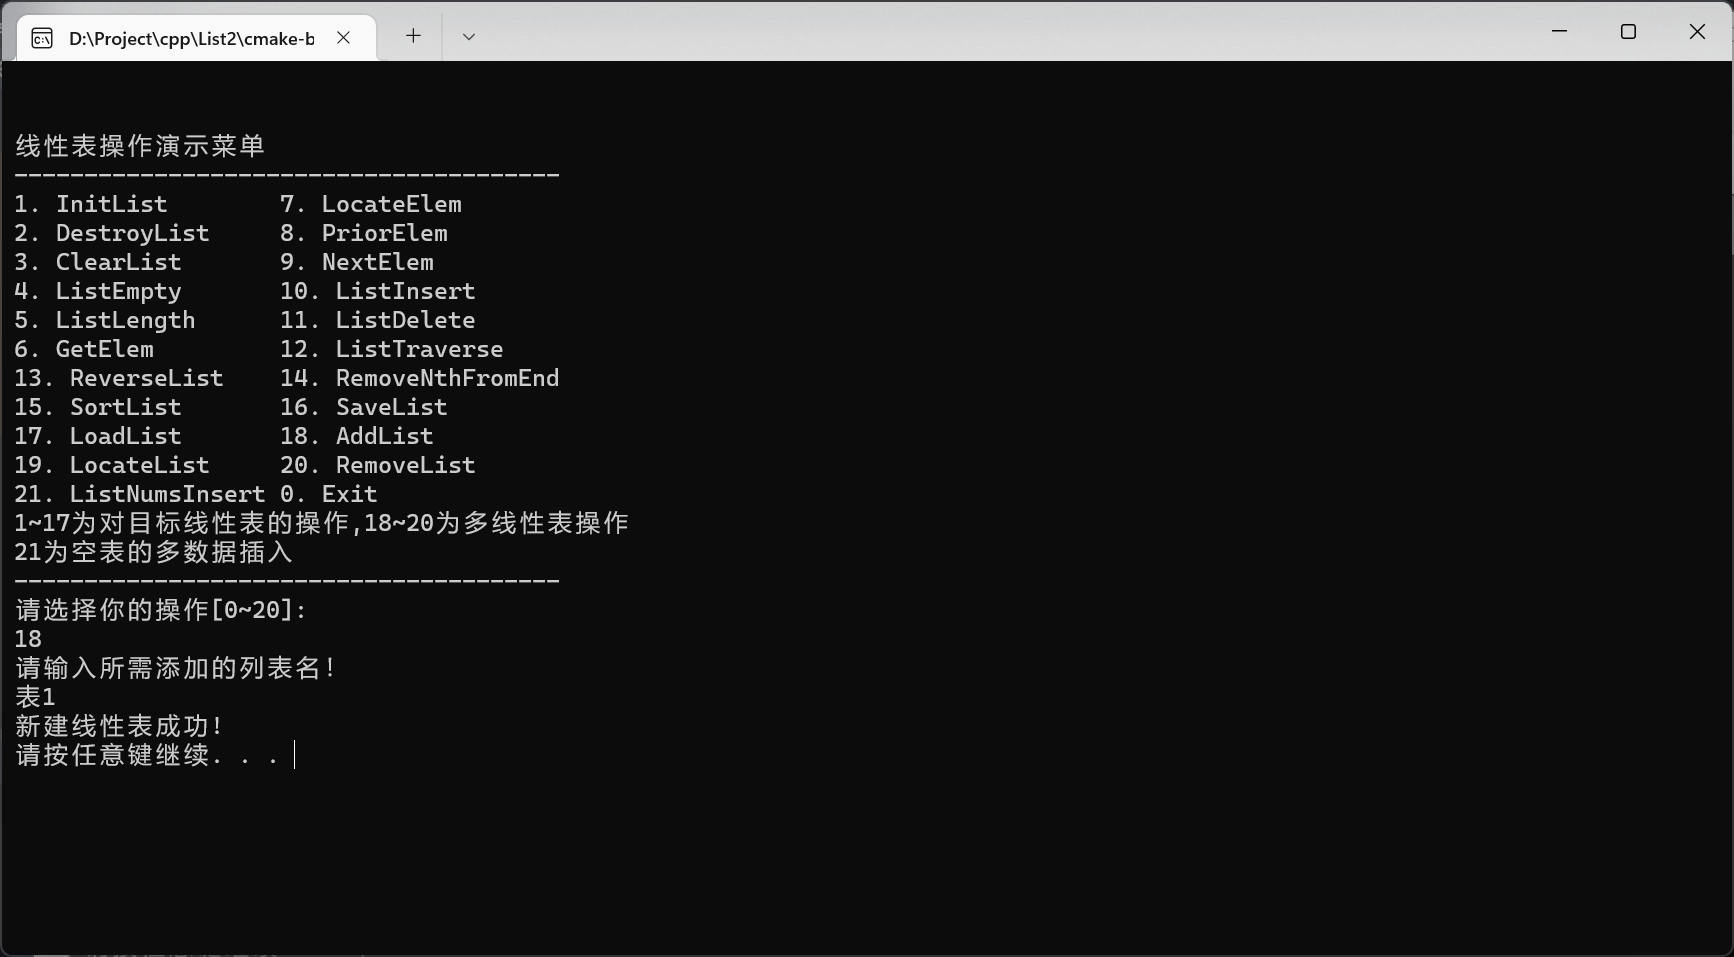
\includegraphics[width=12cm]{images/p1-36.png}}\quad
		      \subfloat[重复表1测试图]{\label{fig1-36}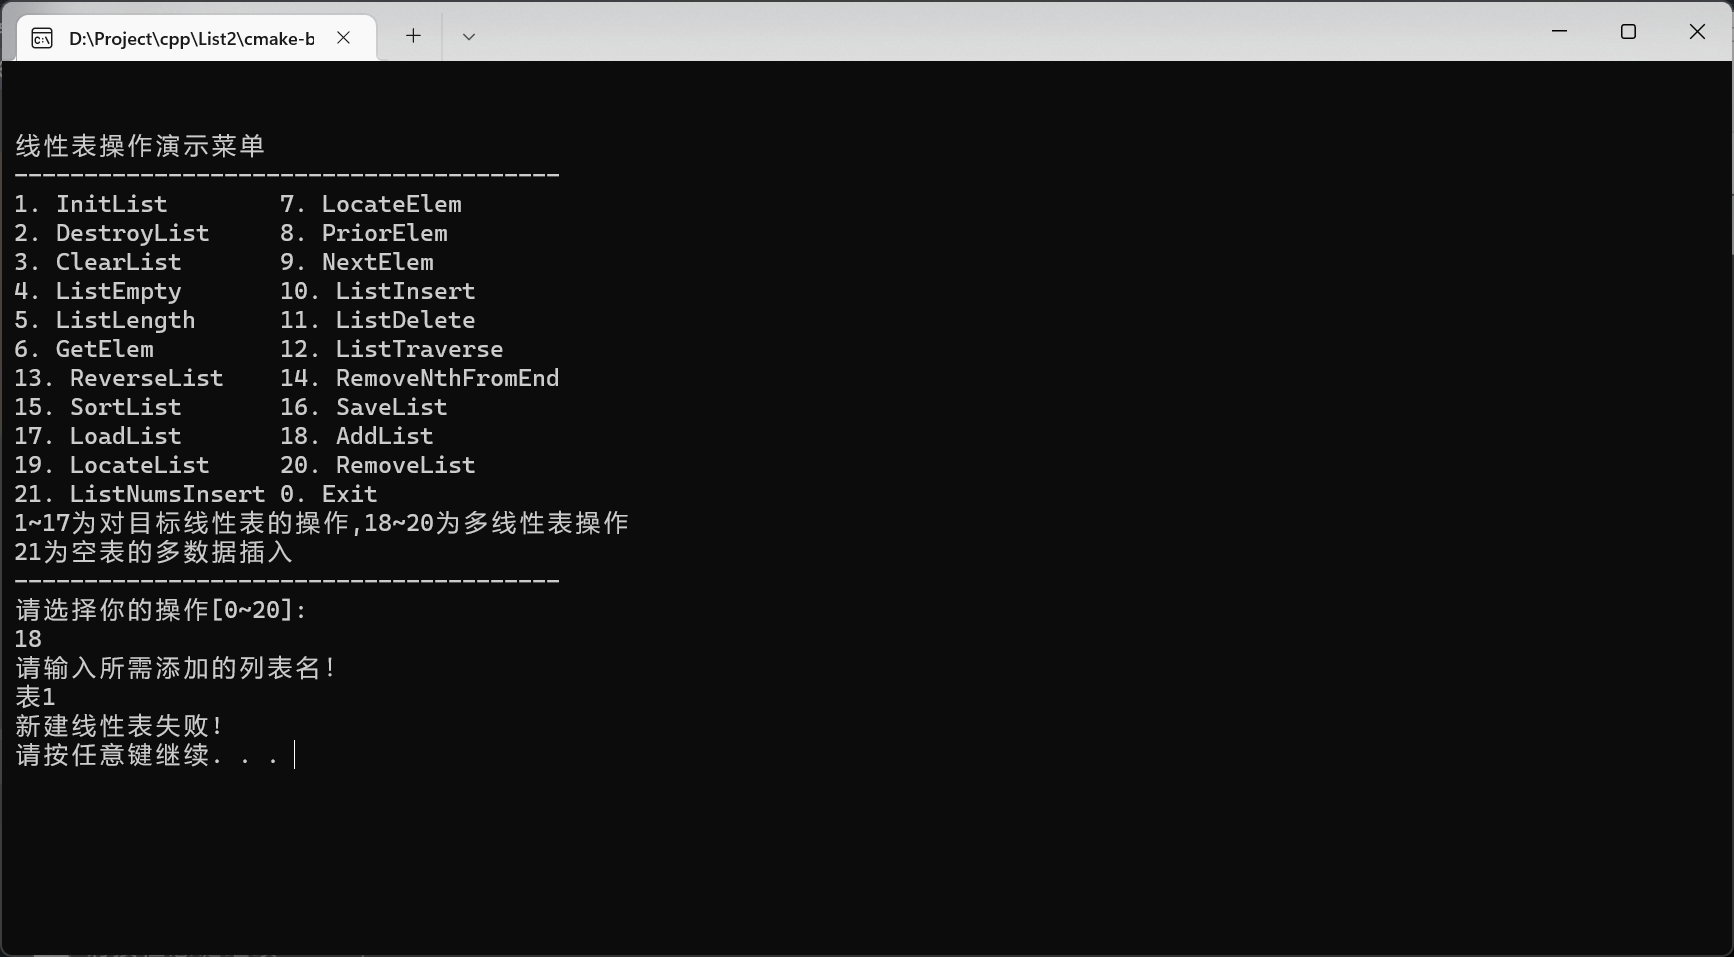
\includegraphics[width=12cm]{images/p1-37.png}}\\
		      \caption{多线性表添加测试}
	      \end{figure}
	      \newpage
	\item LocateLinkList测试
	      \begin{table}[htb]
		      \begin{center}
			      \setlength{\tabcolsep}{2.0mm}
			      \caption{LocateLinkList测试用例表}
			      \label{table20}
			      \begin{tabular}{|c|c|c|c|}
				      \hline
				      测试用例    & 输入             & 理论结果              & 测试结果              \\
				      \hline
				      \hline
				      表1         & 界面选19,输入表1 & 该线性表的位置序号为1 & 该线性表的位置序号为1 \\
				      \hline
				      不存在的表2 & 界面选19,输入表2 & 未找到该线性表        & 未找到该线性表        \\
				      \hline
			      \end{tabular}
		      \end{center}
	      \end{table}
	      \begin{figure}[htb]
		      \centering
		      \subfloat[表1测试图]{\label{fig1-37}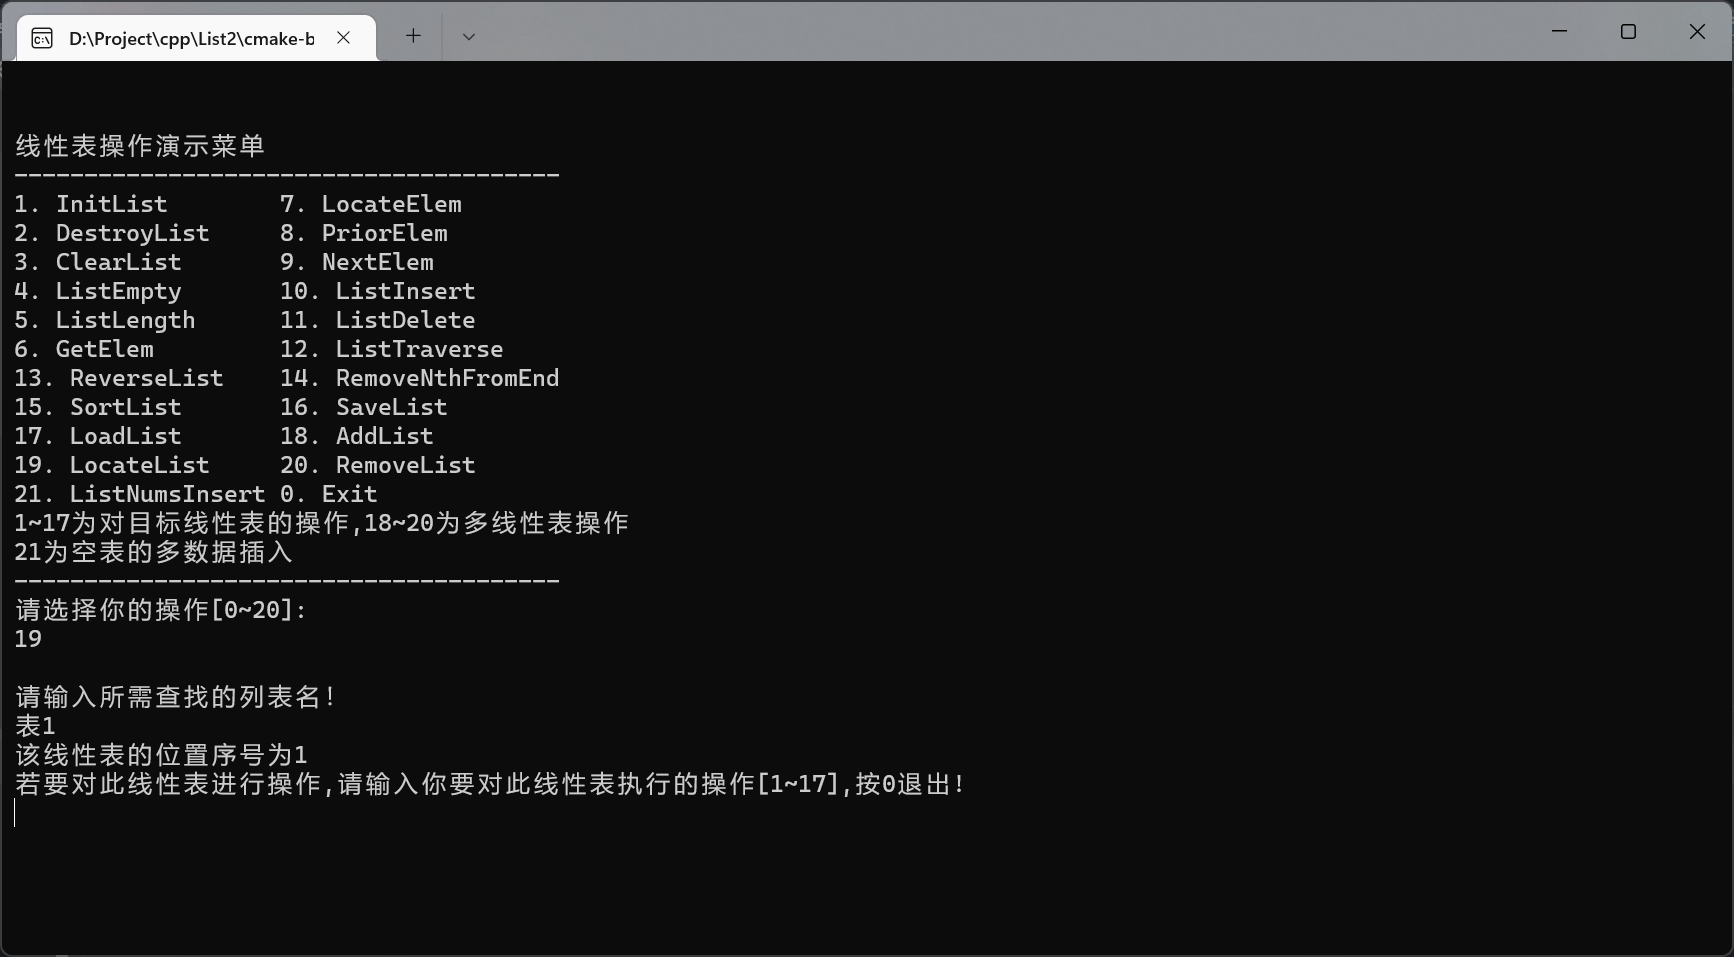
\includegraphics[width=12cm]{images/p1-38.png}}\quad
		      \subfloat[不存在的表2测试图]{\label{fig1-38}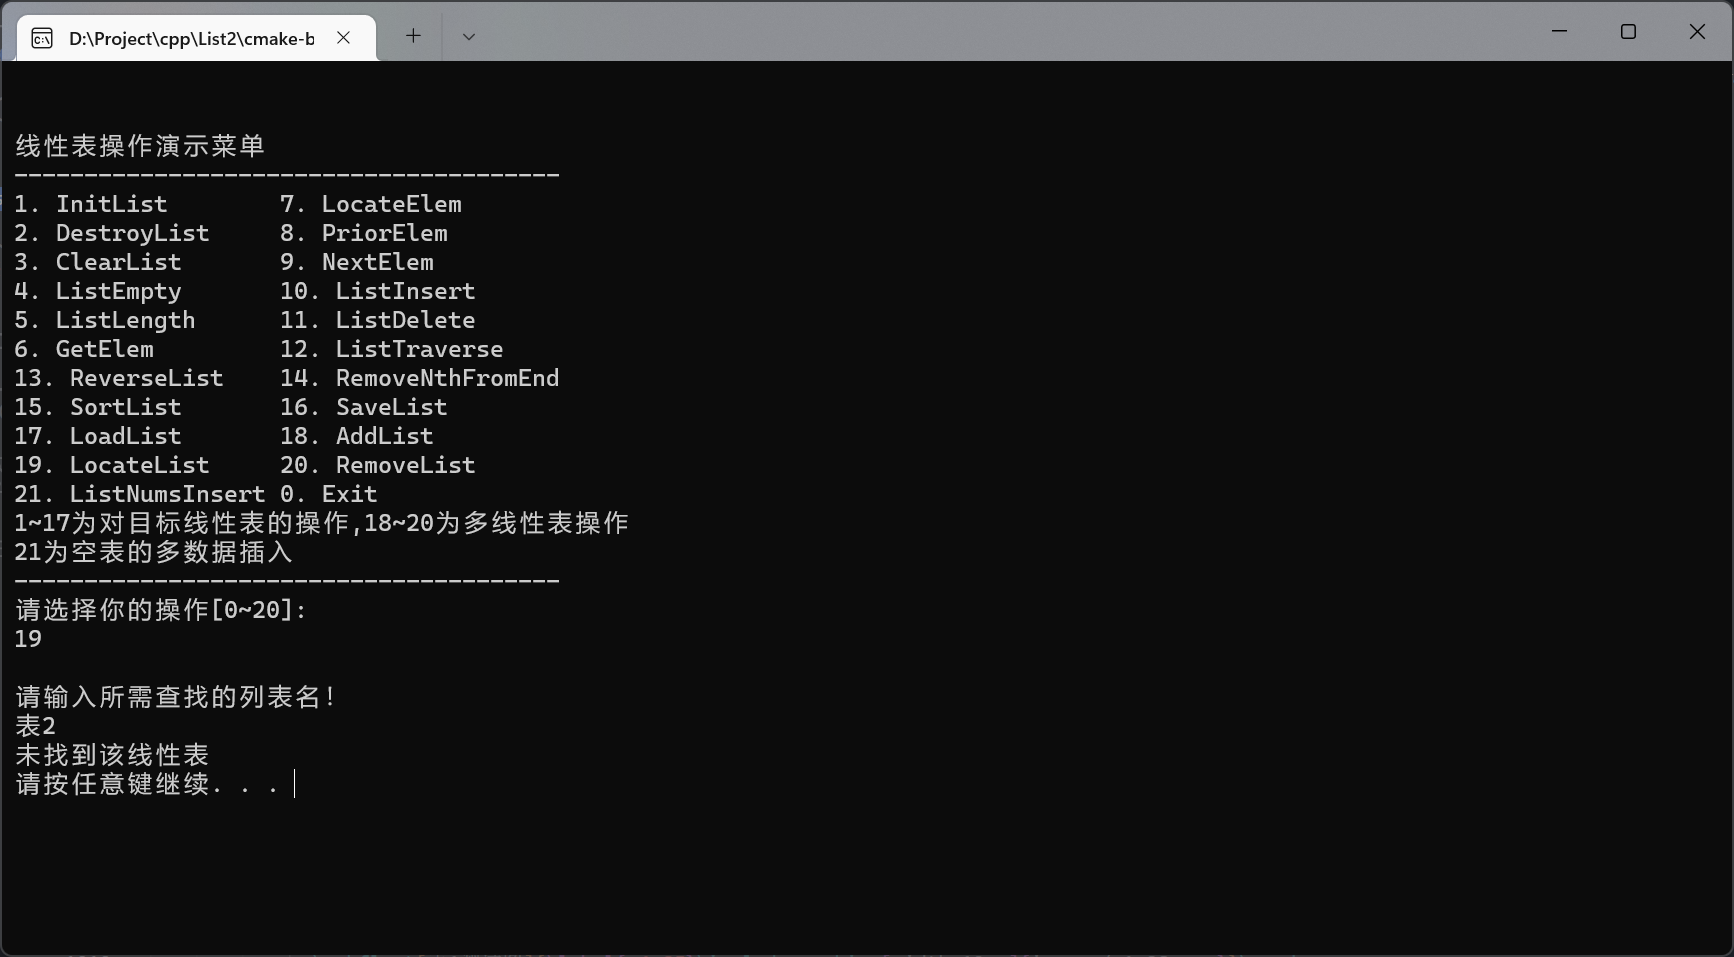
\includegraphics[width=12cm]{images/p1-39.png}}\\
		      \caption{多线性表定位链表测试}
	      \end{figure}
	      \newpage
	\item RemoveList测试
	      \begin{table}[htb]
		      \begin{center}
			      \setlength{\tabcolsep}{2.0mm}
			      \caption{RemoveList测试用例表}
			      \label{table21}
			      \begin{tabular}{|c|c|c|c|}
				      \hline
				      测试用例    & 输入             & 理论结果 & 测试结果 \\
				      \hline
				      \hline
				      表1         & 界面选20,输入表1 & 移除成功 & 移除成功 \\
				      \hline
				      不存在的表2 & 界面选20,输入表2 & 移除失败 & 移除失败 \\
				      \hline
			      \end{tabular}
		      \end{center}
	      \end{table}
	      \begin{figure}[htb]
		      \centering
		      \subfloat[表1测试图]{\label{fig1-39}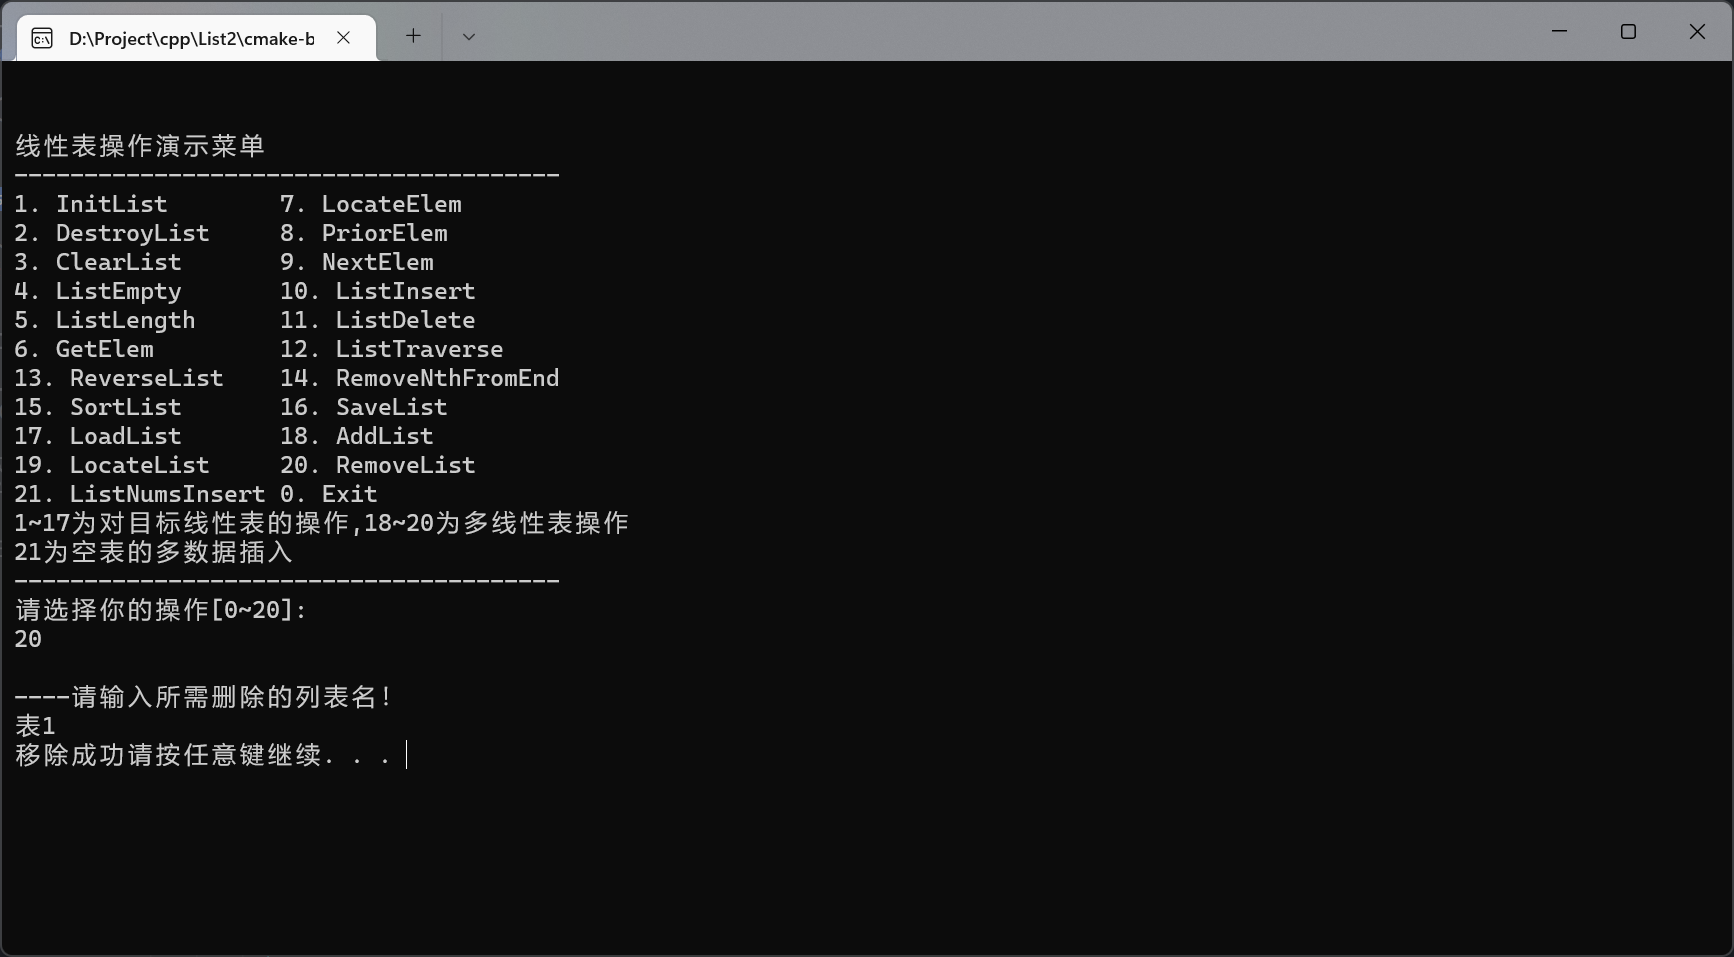
\includegraphics[width=12cm]{images/p1-40.png}}\quad
		      \subfloat[不存在的表2测试图]{\label{fig1-40}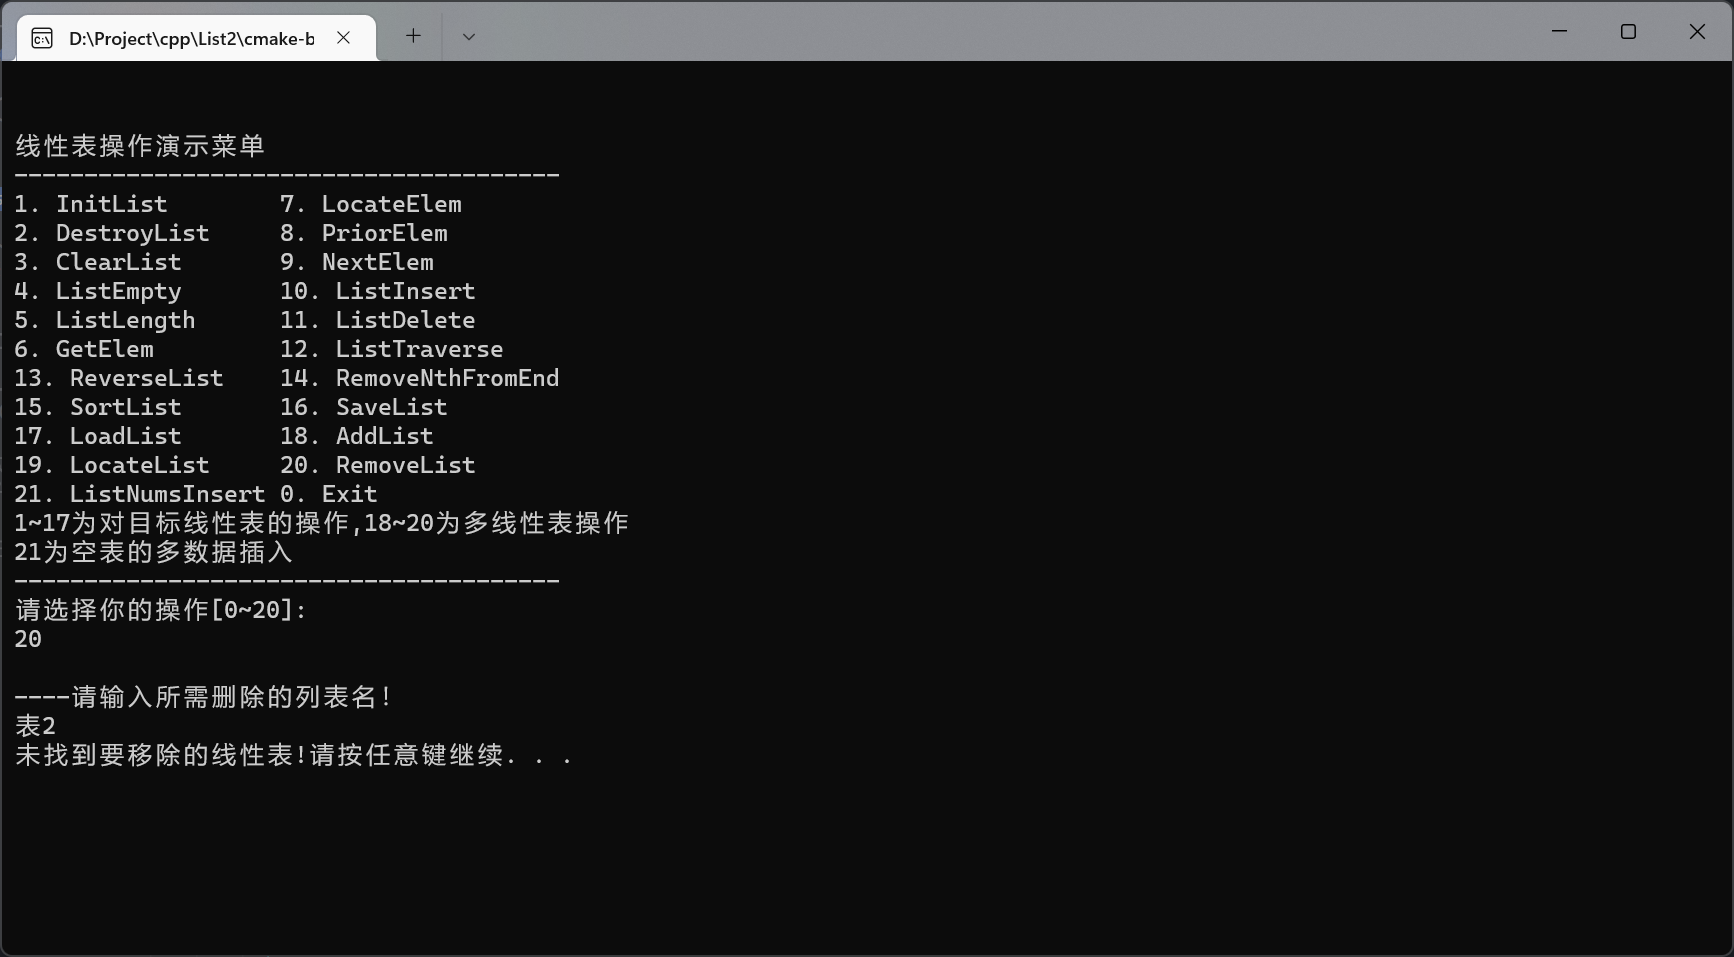
\includegraphics[width=12cm]{images/p1-41.png}}\\
		      \caption{多线性表移除链表测试}
	      \end{figure}
	      \newpage
	\item SaveList测试
	      \begin{table}[htb]
		      \begin{center}
			      \setlength{\tabcolsep}{2.0mm}
			      \caption{SaveList测试用例表}
			      \label{table22}
			      \begin{tabular}{|c|c|c|c|}
				      \hline
				      测试用例   & 输入             & 理论结果     & 测试结果     \\
				      \hline
				      \hline
				      List       & 界面选16,输入表1 & 保存成功     & 保存成功     \\
				      \hline
				      未初始化表 & 界面选16,输入123 & 线性表不存在 & 线性表不存在 \\
				      \hline
				      NULL       & 界面选16,输入123 & 线性表为空   & 线性表为空   \\
				      \hline
			      \end{tabular}
		      \end{center}
	      \end{table}
	      \begin{figure}[htb]
		      \centering
		      \subfloat[未初始化表]{\label{fig1-41}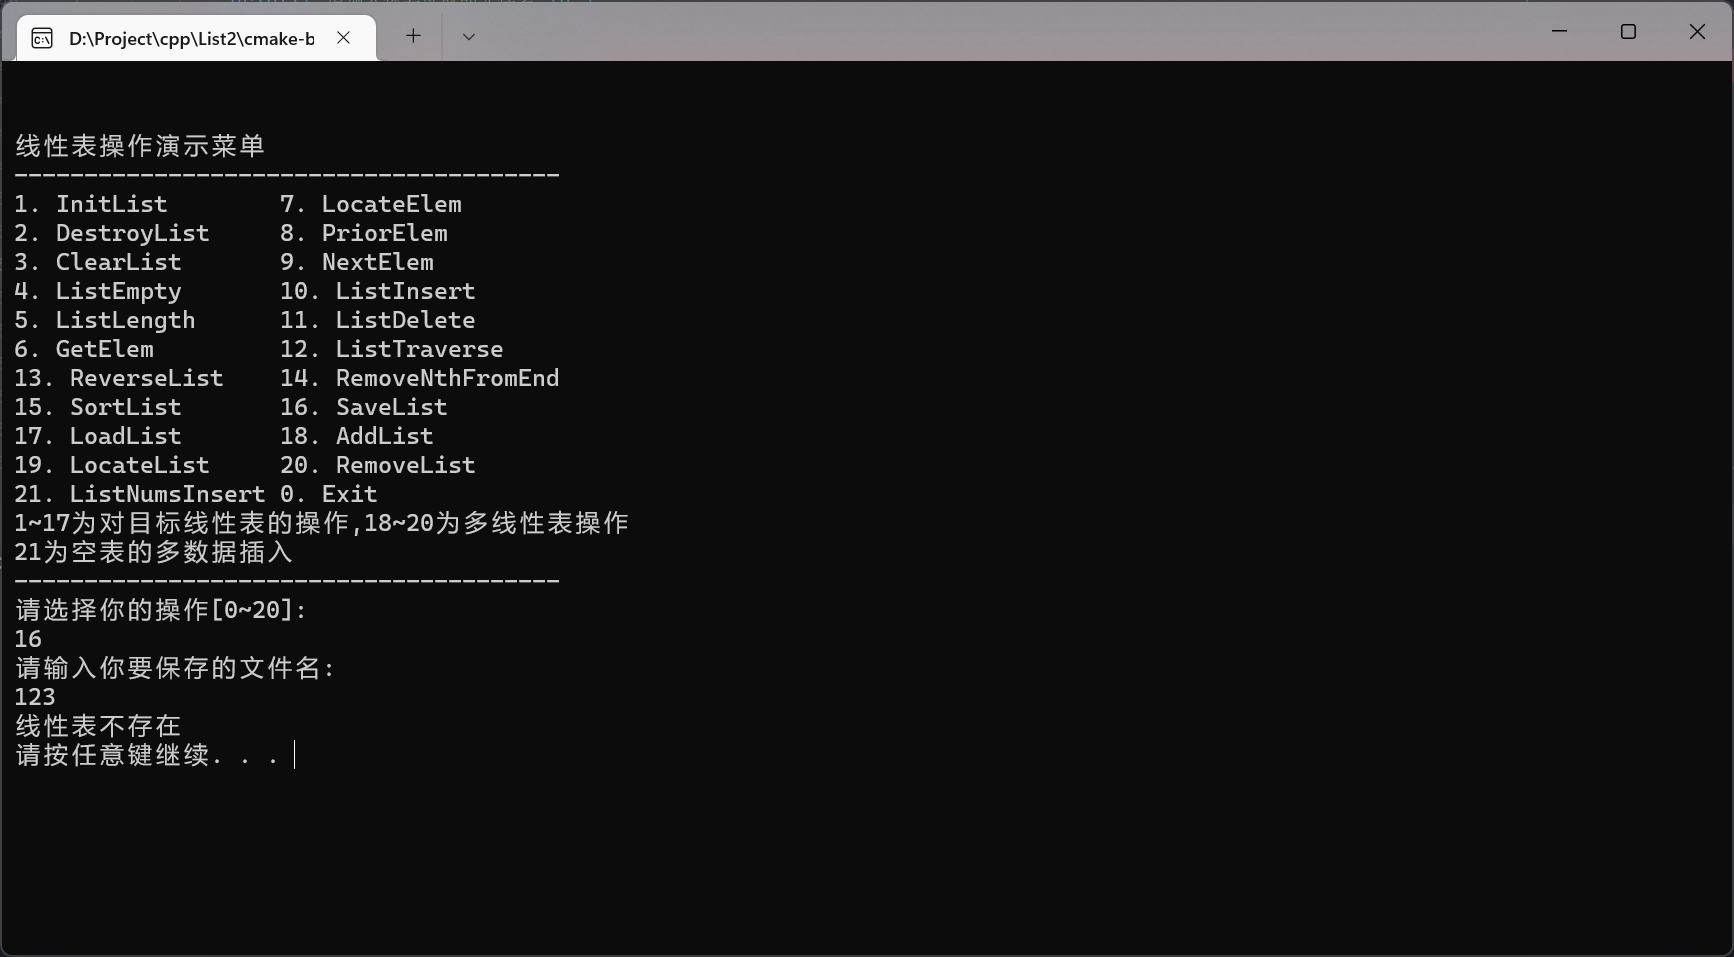
\includegraphics[width=7cm]{images/p1-42.png}}\quad
		      \subfloat[NULL]{\label{fig1-42}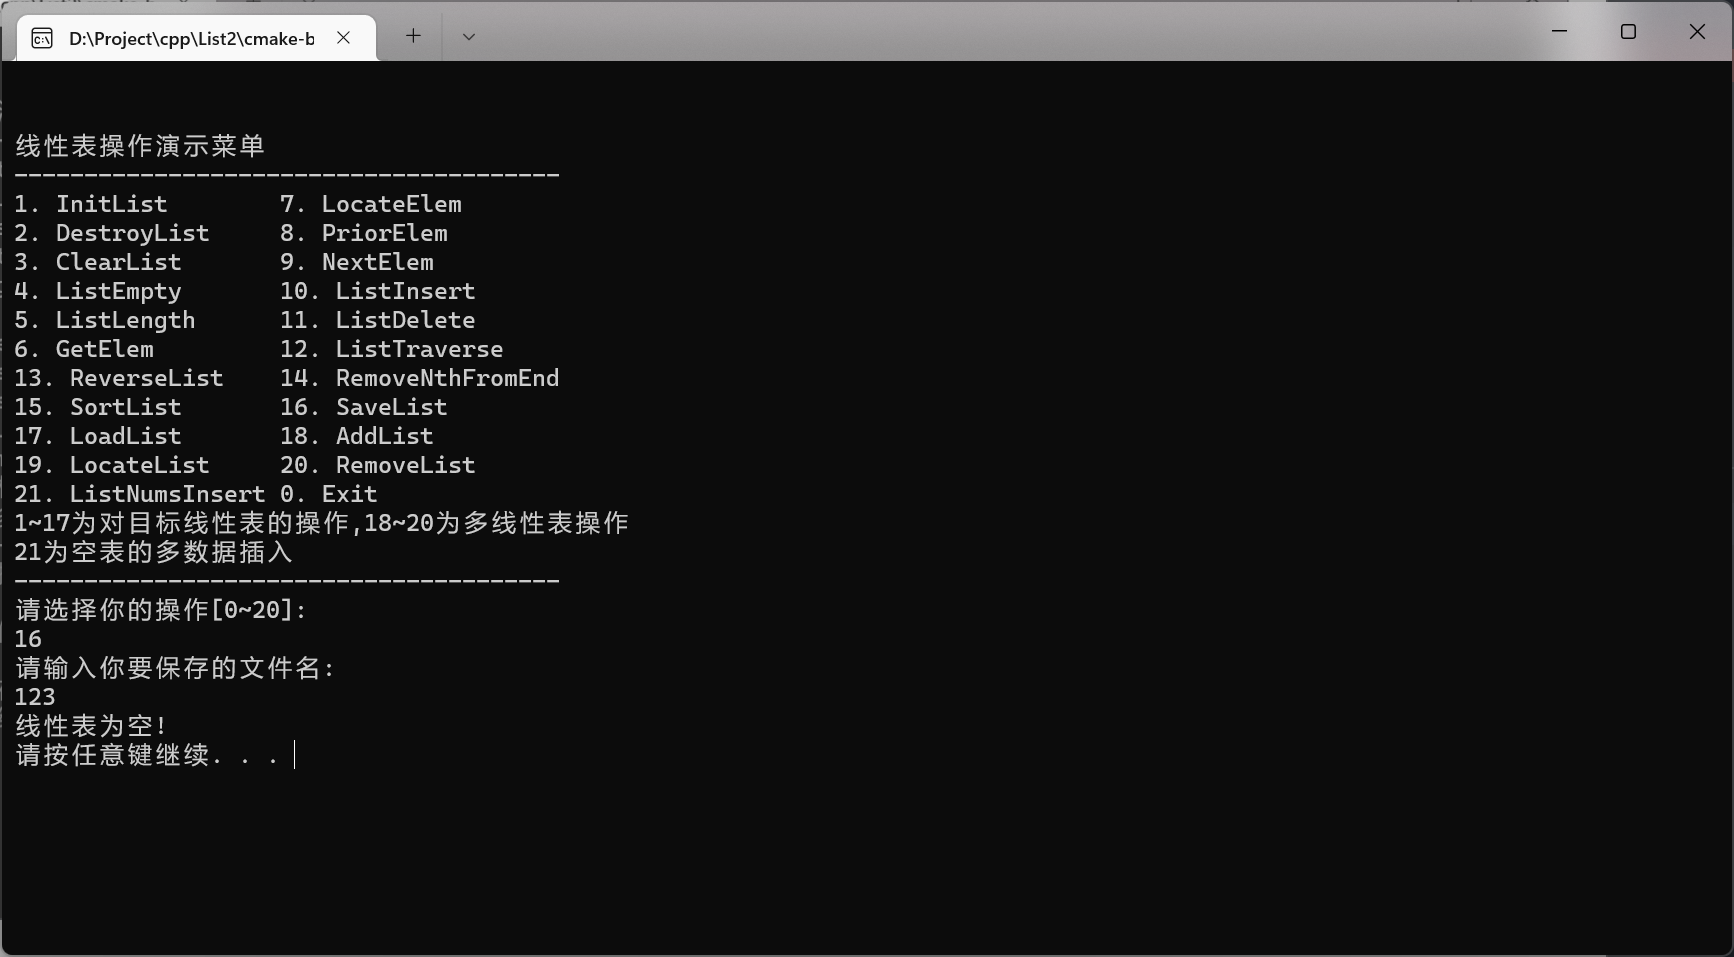
\includegraphics[width=7cm]{images/p1-43.png}}\quad
		      \subfloat[List]{\label{fig1-43}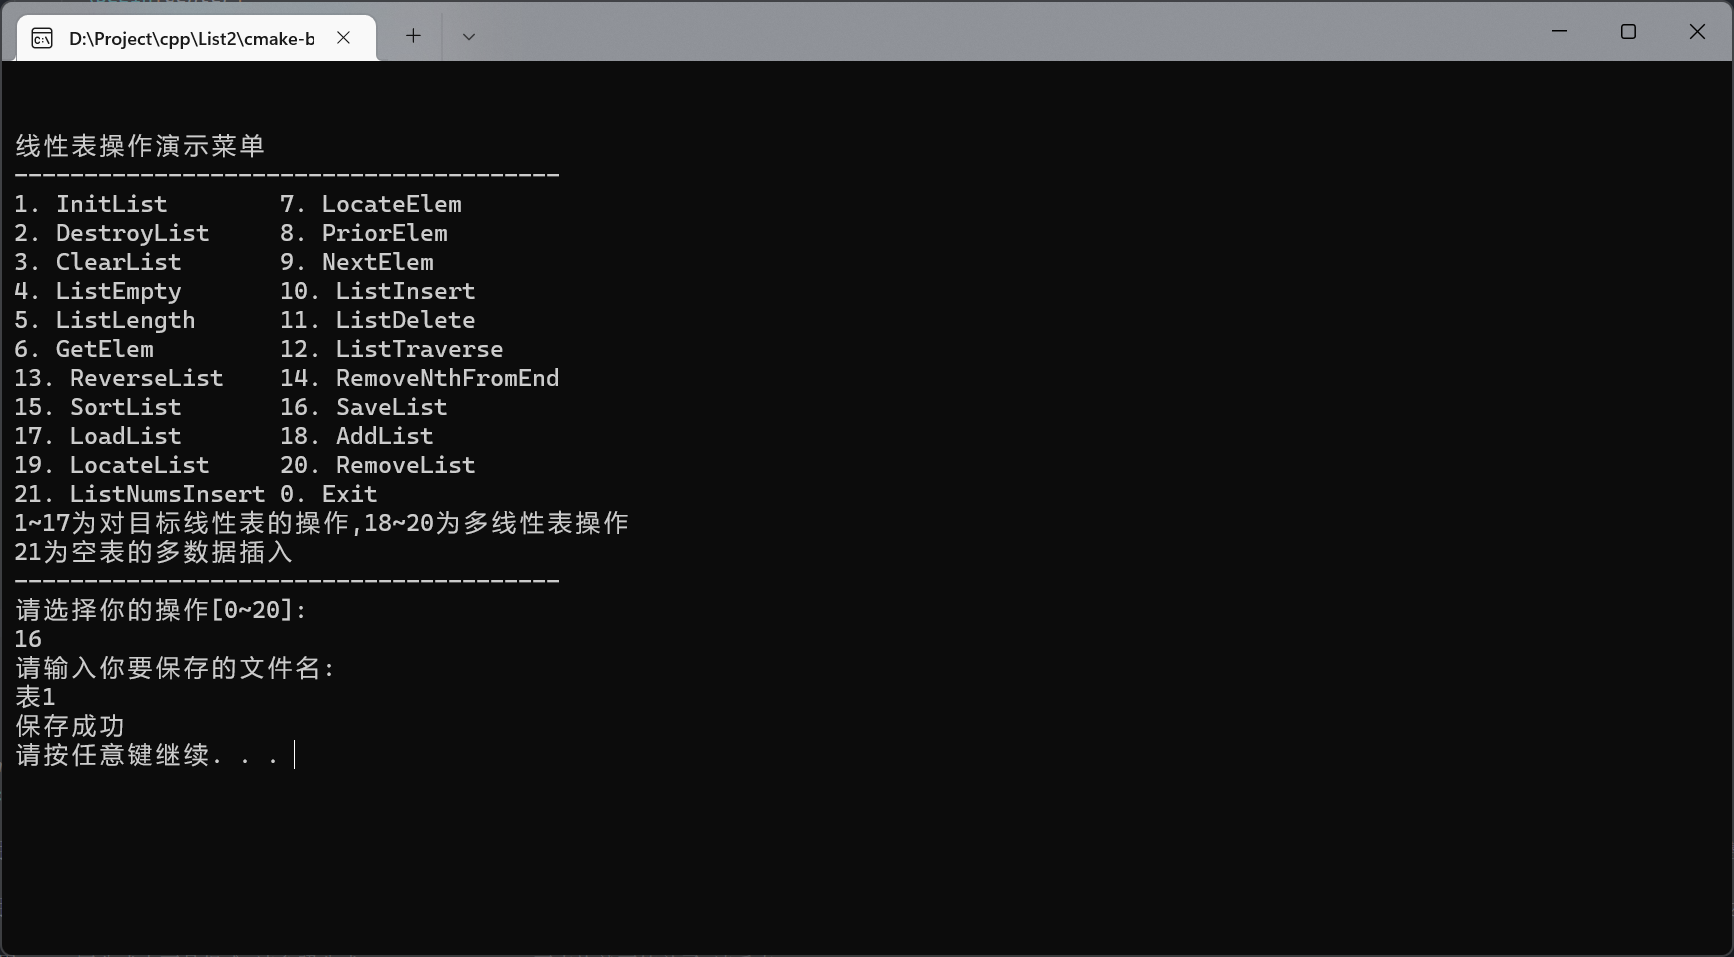
\includegraphics[width=7cm]{images/p1-45.png}}\quad
		      \subfloat[保存的文件]{\label{fig1-44}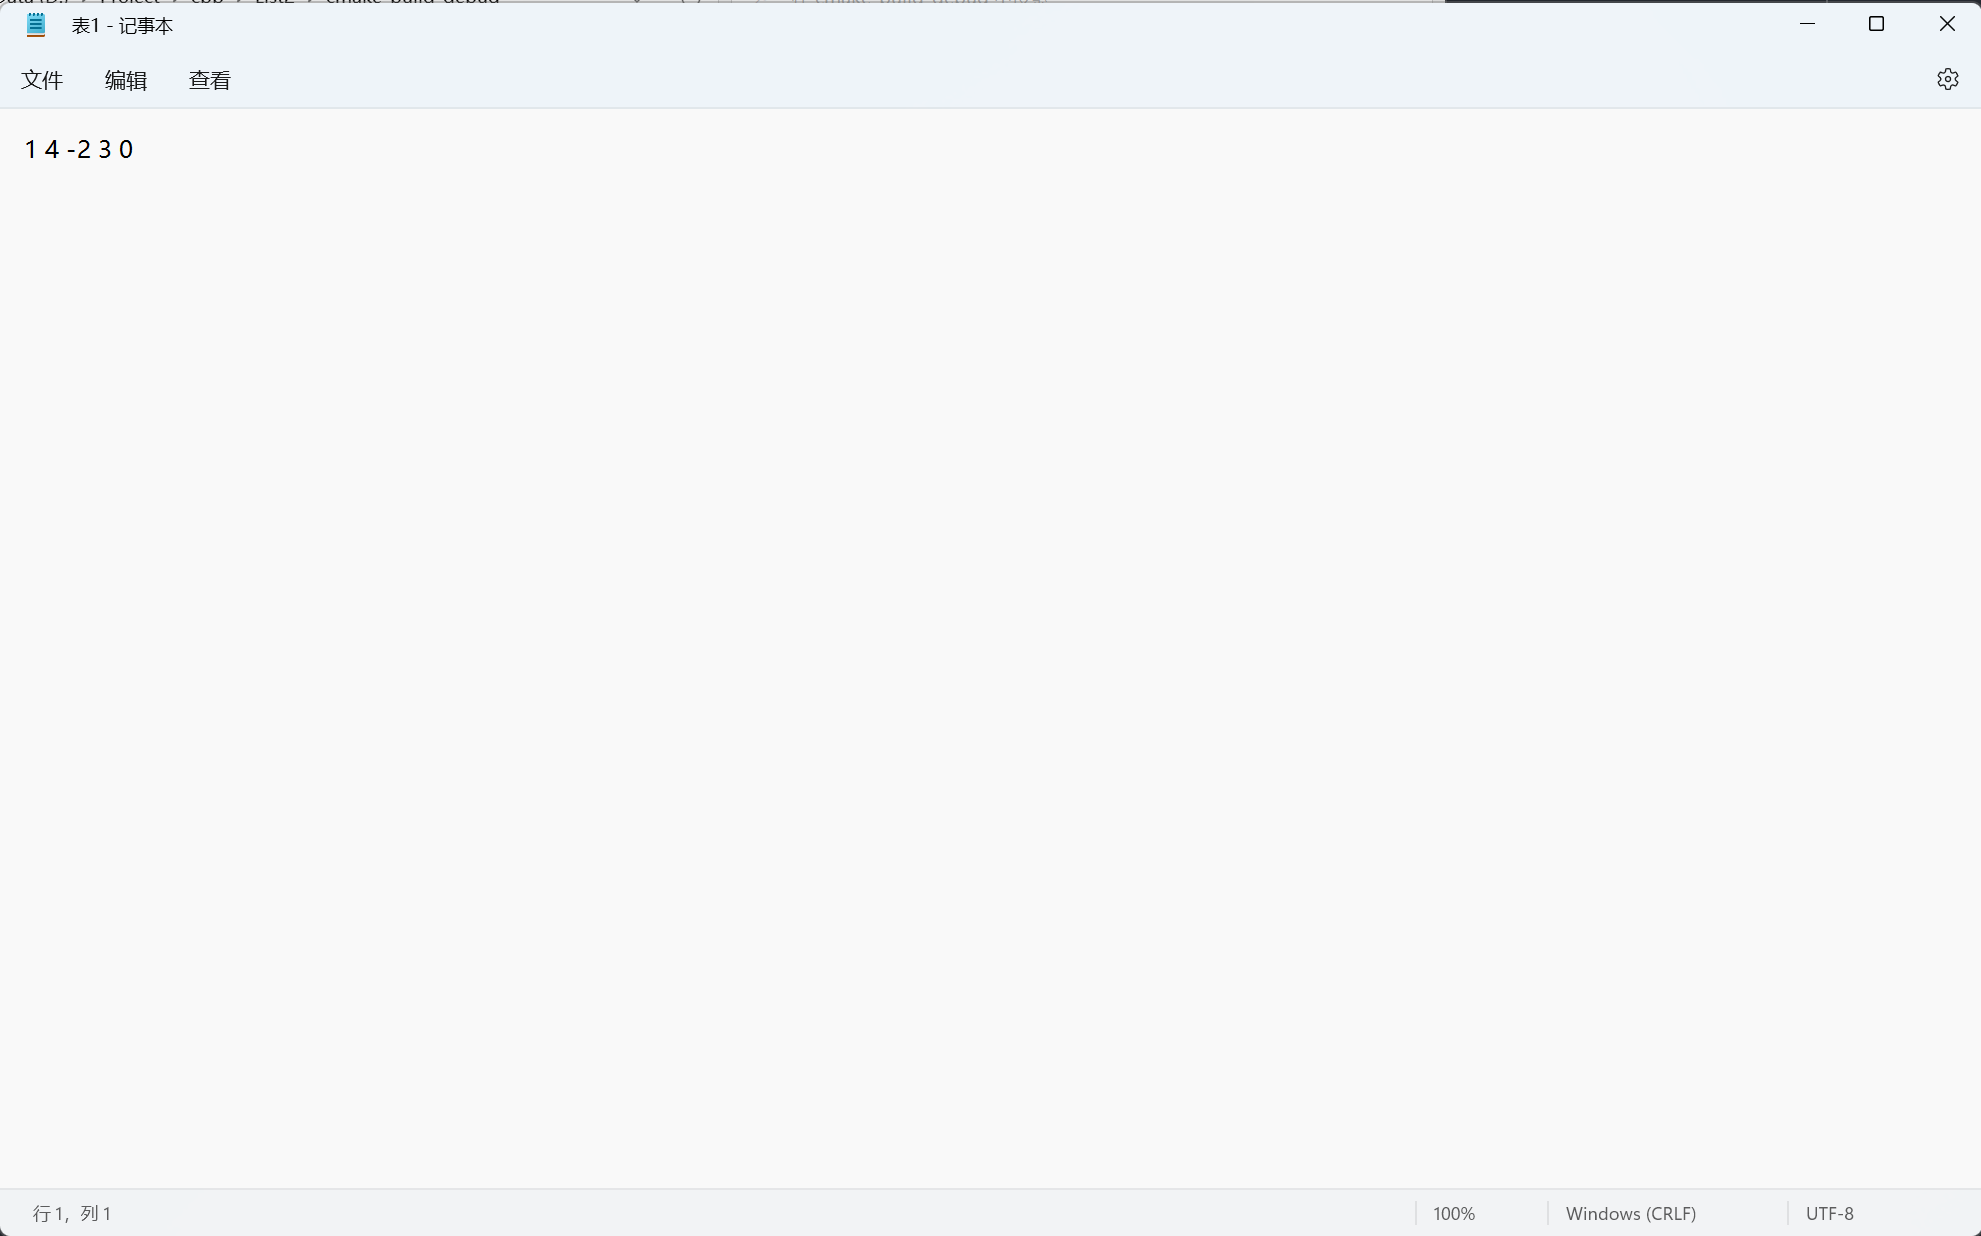
\includegraphics[width=7cm]{images/p1-44.png}}\\
		      \caption{保存文件测试}
	      \end{figure}
	      \newpage
	\item LoadList测试
	      \begin{table}[htb]
		      \begin{center}
			      \setlength{\tabcolsep}{2.0mm}
			      \caption{LoadList测试用例表}
			      \label{table23}
			      \begin{tabular}{|c|c|c|c|}
				      \hline
				      测试用例   & 输入                  & 理论结果     & 测试结果      \\
				      \hline
				      \hline
				      未初始化表 & 界面选17,输入表1      & 读取成功     & 读取成功      \\
				      \hline
				      未初始化表 & 界面选17,输入没有的表 & 读取失败     & 读取失败      \\
				      \hline
				      NULL       & 界面选17              & 线性表已存在 & 线性表L已存在 \\
				      \hline
			      \end{tabular}
		      \end{center}
	      \end{table}
	      \begin{figure}[htb]
		      \centering
		      \subfloat[未初始化表1]{\label{fig1-45}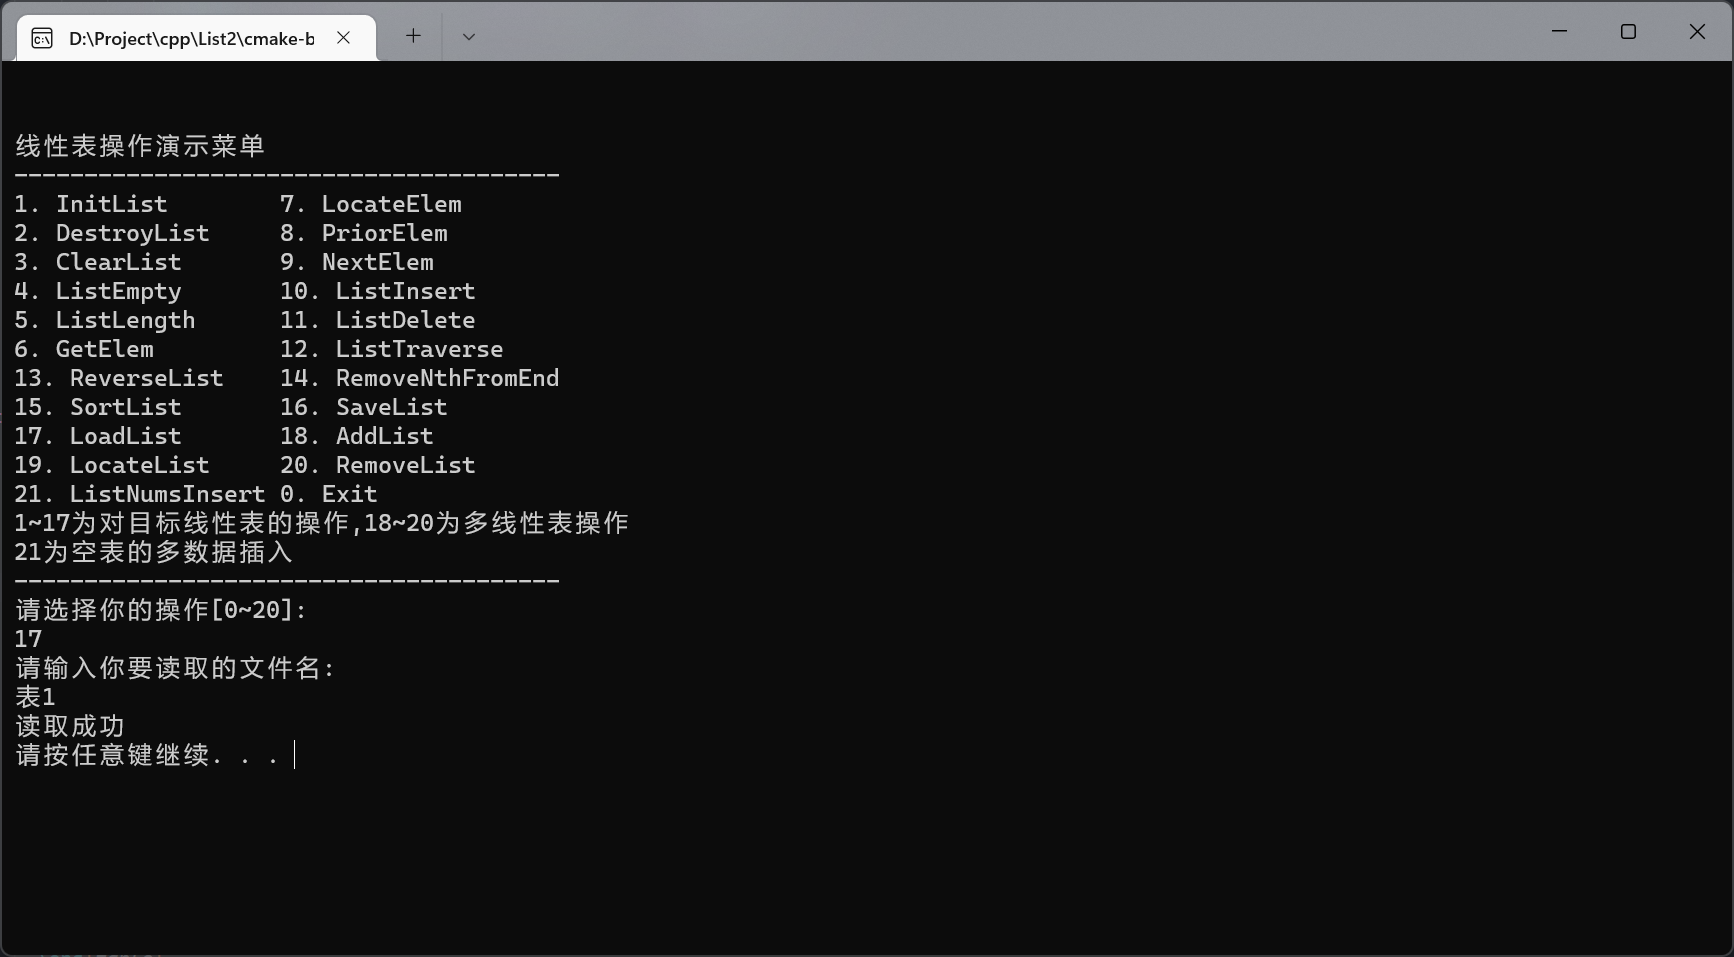
\includegraphics[width=7cm]{images/p1-46.png}}\quad
		      \subfloat[没有的表]{\label{fig1-46}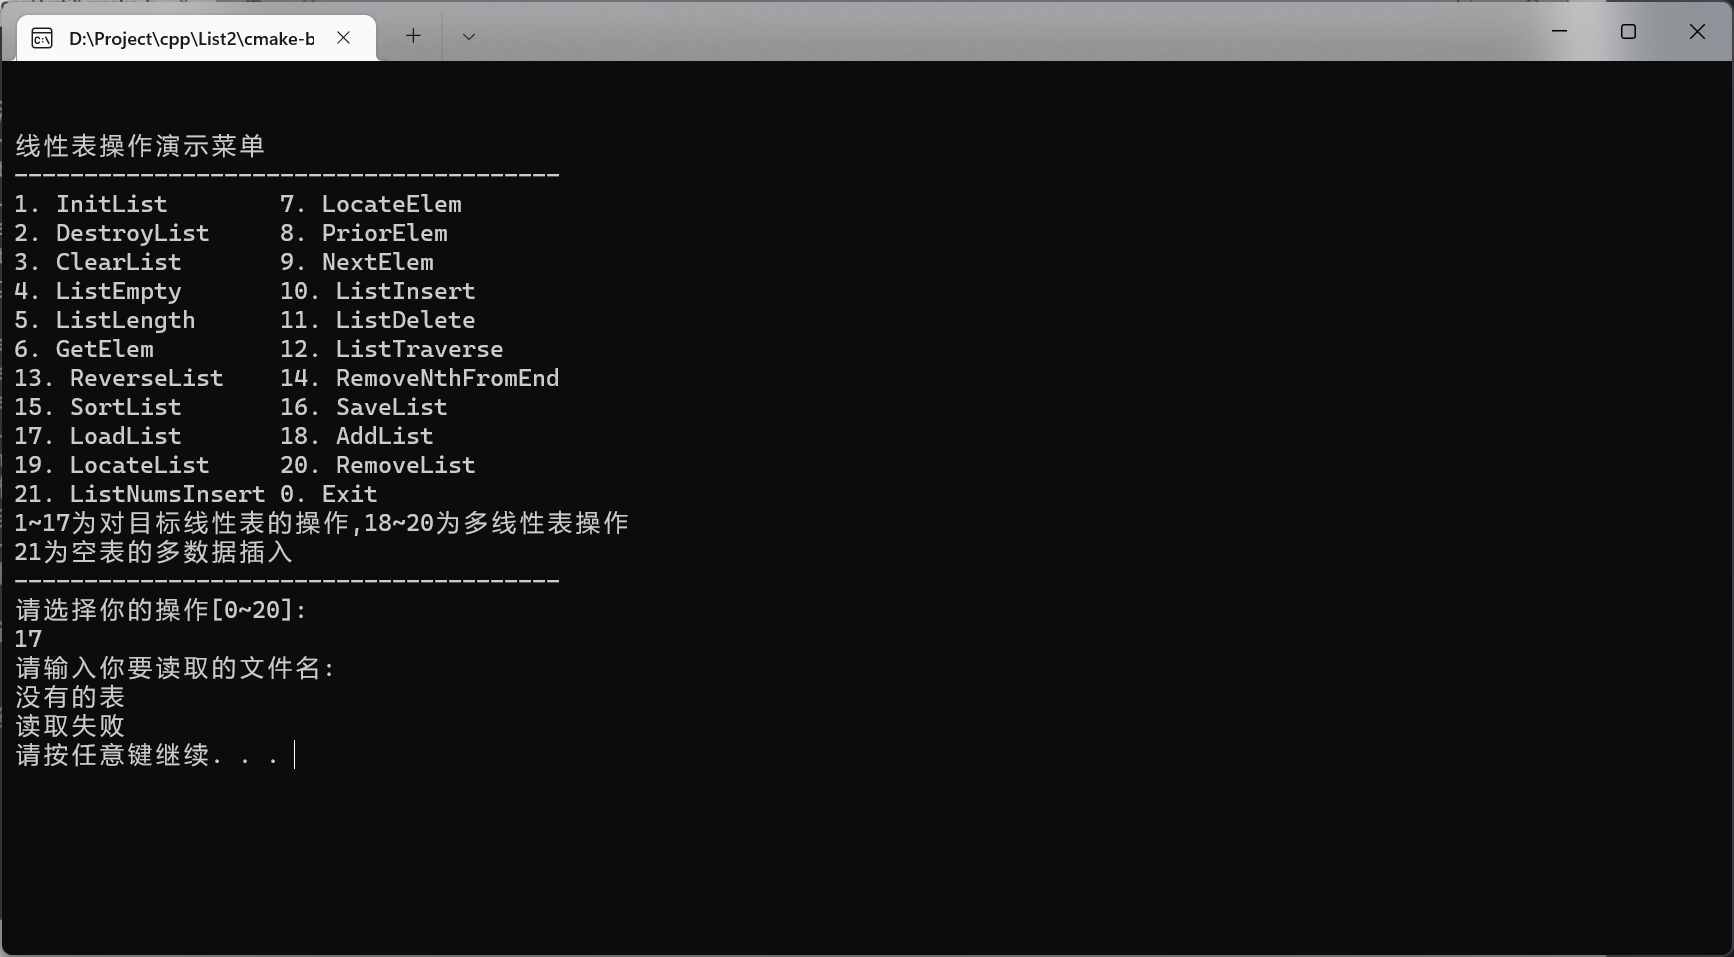
\includegraphics[width=7cm]{images/p1-47.png}}\quad
		      \subfloat[NULL]{\label{fig1-47}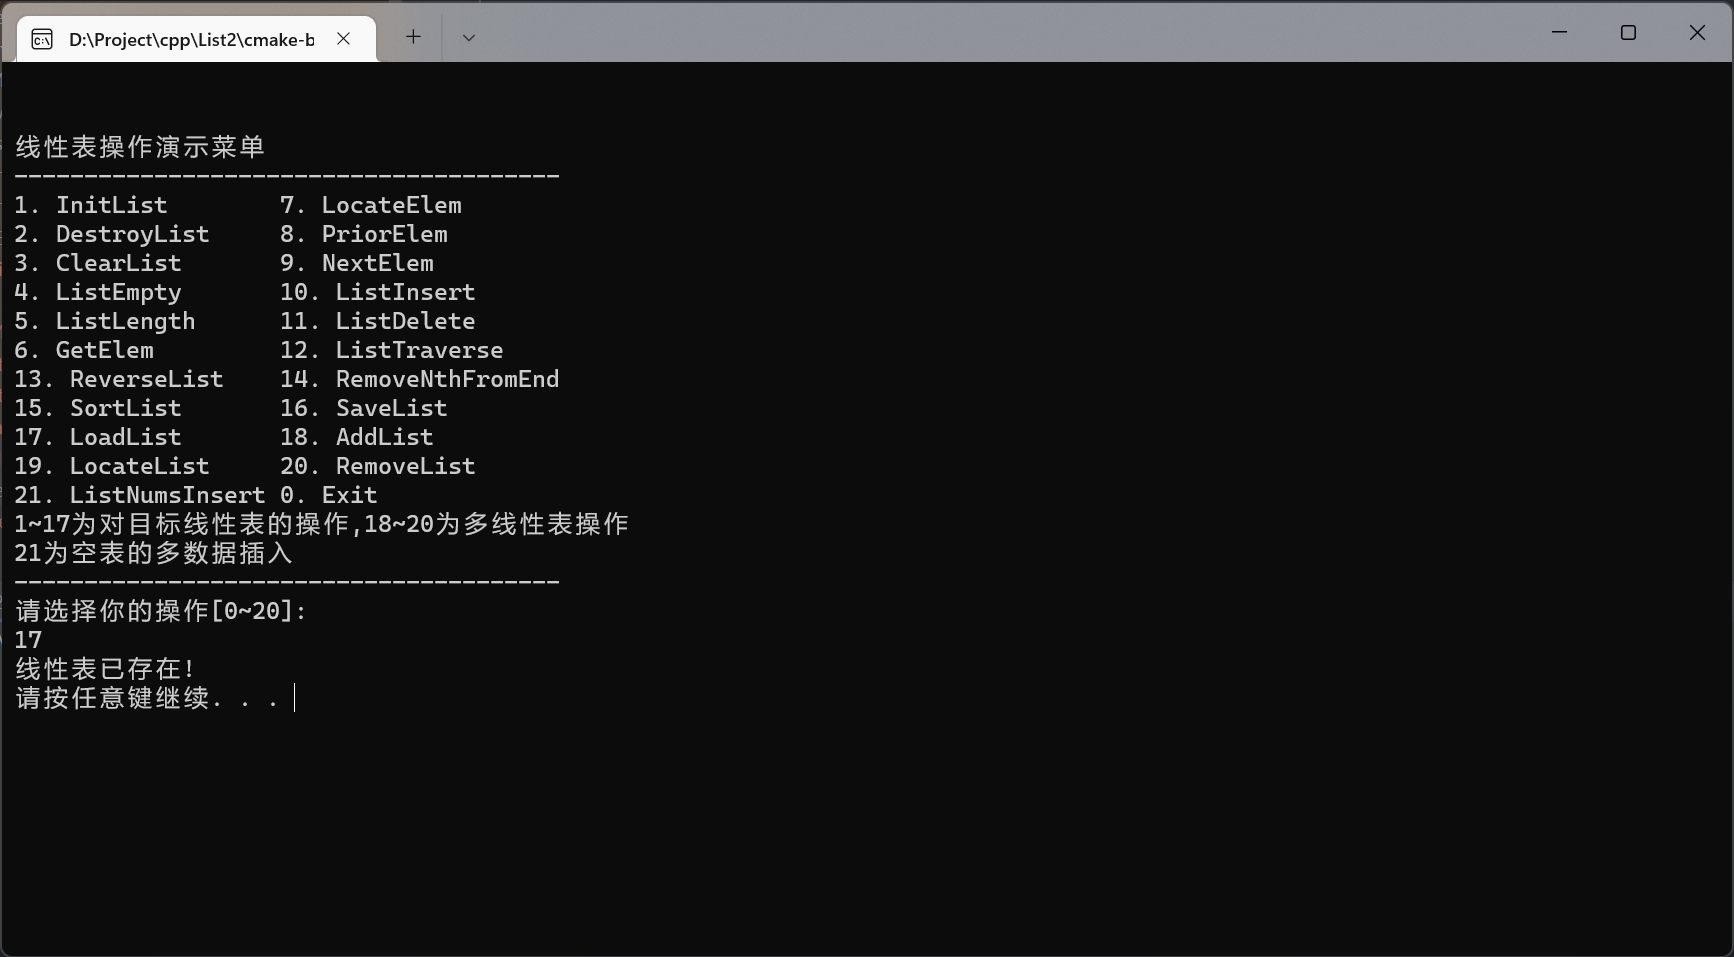
\includegraphics[width=12cm]{images/p1-48.png}}\\
		      \caption{保存文件测试}
	      \end{figure}
\end{enumerate}
\newpage
\subsection{实验小结}


\newpage
\section{基于邻接表的图实现}



\subsection{问题描述}
实验目的:
以邻接表结构构造无向图,创建一个简易菜单的功能演示界面,该演示系统可选择实现多个线性表管理。需要在主程序中完成函数调用以及所需实参值和函数执行结果
的输出,以函数形式定义创建图、销毁图、查找顶点、获得顶点值和顶点赋值等12种基本运算以及找到距离小于k的顶点集合,获取顶点间最短路径和长度,获取图的连通分量等附加功能,
并给出了相应的操作提示。并且可选择以文件的形式进行存储和加载。\\
实验目标:\\
1:\quad 加深对图的概念、基本运算的理解\\
2:\quad 熟练掌握图的逻辑结构与物理结构的关系\\
3:\quad 以邻接表作为物理结构,熟练掌握图基本运算的实现\\
实现函数:
\begin{enumerate}[label =\color{red} (\arabic*)]
	\item CreateGraph(G,V,VR)创建图\quad 函数位置: \ref{G1}
	\item DestroyGraph(G)销毁图\quad 函数位置: \ref{G2}
	\item LocateVex(G,u)查找顶点\quad 函数位置: \ref{G3}
	\item PutVex(G,u,value)顶点赋值\quad 函数位置: \ref{G4}
	\item FirstAdjVex(G, u)获得第一邻接点\quad 函数位置: \ref{G5}
	\item NextAdjVex(G, v, w)获得下一邻接点\quad 函数位置: \ref{G6}
	\item InsertVex(G,v)插入顶点\quad 函数位置: \ref{G7}
	\item DeleteVex(G,v)删除顶点\quad 函数位置: \ref{G8}
	\item InsertArc(G,v,w)插入弧\quad 函数位置: \ref{G9}
	\item DeleteArc(G,v,w)删除弧\quad 函数位置: \ref{G10}
	\item DFSTraverse(G,visit())深度优先搜索遍历\quad 函数位置: \ref{G11}
	\item BFSTraverse(G,visit())广度优先搜索遍历\quad 函数位置: \ref{G12}
	\item VerticesSetLessThanK(G,v,k)获取距离小于k的顶点集合\quad 函数位置: \ref{G13}
	\item ShortestPathLength(G,v,w)获取顶点间最短路径和长度\quad 函数位置: \ref{G15}
	\item ConnectedComponentsNums(G)获取图的连通分量\quad 函数位置: \ref{G16}
	\item SaveGraph(G,FileName)将图保存在FileName文件中\quad 函数位置: \ref{G17}
	\item LoadGraph(G,FileName)将FileName中的图加载出来\quad 函数位置: \ref{G18}
	\item AddGraph(Graphs,GraphName)在Graphs中添加名为GraphName的图
	\item RemoveGraph(Graphs,GraphName)在Graphs中移除名为GraphName的图\quad 函数位置: \ref{G19}
	\item LocateGraph(Graphs,GraphName) 在Graphs中查找名为GraphName的图,输出其序号,并选择是否要调用function函数对此表进行操作\quad 函数位置: \ref{G20}
\end{enumerate}
\subsection{系统设计}
物理结构为邻接表,创建一个简易菜单的功能演示界面。\\
菜单可选择的操作有:创建图,销毁图,查找顶点,顶点赋值,获得第一邻接点,获得下一邻接点,插入顶点,删除顶点,插入弧,删除弧,深度优先搜索遍历,广度优先搜索遍历,获取距离小于k的顶点集合,获取顶点间最短路径和长度,获取图的连通分量,文件保存和加载,多图管理\\
程序源代码见附录B\ref{sec:附录d-基于邻接表图实现的源程序}
\subsection{系统实现}
\begin{enumerate}
	\renewcommand{\labelenumi}{Code:\theenumi}
	\item 函数名称:CreateCraph(\&G,V,VR)\\
	      初始条件:V是图的顶点集,VR是图的关系集\\
	      操作结果:按V和VR的定义构造图G。
	      算法思路:采用邻接表作为物理结构,以V构建顶点集,以VR创建每条边的关系.
	      \begin{algorithm}[htb]
		      \caption{创建图}
		      \begin{algorithmic}[1]
			      \State 开始
			      \State 以V构建顶点集,保证顶点个数不为0以及没有相同顶点
			      \State 以VR创建每条边的关系,根据两个顶点是否已经有第一条弧来选择构建弧的方式
			      \State 结束
		      \end{algorithmic}\label{G1}
	      \end{algorithm}
	\item 函数名称:DestroyGraph(G)\\
	      初始条件:图G已存在\\
	      操作结果:销毁图G\\
	      算法思路:遍历图,依次释放存储数据元素的空间,名称置为空,最后将图的几个顶点数、弧数和种类均置为零
	      \begin{algorithm}[htb]
		      \title{销毁图}
		      \caption{销毁图}
		      \begin{algorithmic}[1]
			      \State 开始
			      \State 依次释放数据存储空间,名称置为空
			      \State 顶点数、弧数和种类均置为零
			      \State 结束
		      \end{algorithmic}\label{G2}
	      \end{algorithm}
	      \newpage
	\item 函数名称:LocateVex(G,u)
	      初始条件:图G存在,u和G中的顶点具有相同特征
	      操作结果:若u在图G中存在,返回顶点u的位置信息,否则返回表示"不存在"其它信息
	      算法思路:遍历图,当图中顶点的值与所给信息的值相同时返回该顶点的key,完成定位
	      \begin{algorithm}[htb]
		      \caption{查找顶点}
		      \begin{algorithmic}[1]
			      \State 开始
			      \State 遍历图
			      \State 图中顶点的值与所给信息的值相同时,返回该顶点的key
			      \State 结束
		      \end{algorithmic}\label{G3}
	      \end{algorithm}
	\item 函数名称:PutVex (G,v,value)\\
	      初始条件:图G存在,v是G中的某个顶点\\
	      操作结果:对v赋值value\\
	      算法思路:调用LocateVex(G,u)函数,在保证关键字和名称唯一的前提下将找到的顶点的值修改为所给值
	      \begin{algorithm}[htb]
		      \title{顶点赋值}
		      \caption{顶点赋值}
		      \begin{algorithmic}[1]
			      \State 开始
			      \State 调用LocateVex(G,v)函数
			      \State 保存该顶点value,对该顶点赋值
			      \State 检查关键字是否唯一,不唯一则将该顶点的值回滚,反之完成赋值操作
			      \State 结束
		      \end{algorithmic}\label{G4}
	      \end{algorithm}
	\item 函数名称:FirstAdjVex(\&G, v)\\
	      初始条件:图G存在,v是G的一个顶点\\
	      操作结果:返回v的第一个邻接顶点,如果v没有邻接顶点,返回表示"不存在"其它信息\\
	      算法思路:调用LocateVex(G,u)函数,并返回找到的顶点的第一个邻接顶点
	      \newpage
	      \begin{algorithm}[htb]
		      \title{第一邻接点}
		      \caption{第一邻接点}
		      \begin{algorithmic}[1]
			      \State 开始
			      \State 调用LocateVex(G,v)函数,找到目标顶点
			      \State 判该顶点的firstarc是否为空,若为空返回-1
			      \State 返回找到的顶点的第一个邻接顶点
			      \State 函数结束
		      \end{algorithmic}\label{G5}
	      \end{algorithm}
	\item 函数名称:NextAdjVex(\&G, v, w)\\
	      初始条件:图G存在,v是G的一个顶点,w是v的邻接顶点\\
	      操作结果:返回v的(相对于w)下一个邻接顶点,如果w是最后一个邻接顶点,返回表示"不存在"其它信息\\
	      算法思路:调用LocateVex(G,u)函数,并返回找到的顶点相对所给的邻接顶点的下一个邻接顶点。
	      \begin{algorithm}[htb]
		      \title{相对邻接点}
		      \caption{相对邻接点}
		      \begin{algorithmic}[1]
			      \State 开始
			      \State 调用LocateVex(G,V)函数,找到目标顶点
			      \State 遍历目标顶点所有弧,找到相对邻接顶点
			      \State 判断下一邻接顶点是否为空
			      \State 若不为空,则返回该顶点位序,反之返回"不存在"
			      \State 结束
		      \end{algorithmic}\label{G6}
	      \end{algorithm}
	\item 函数名称:InsertVex(\&G,v)\\
	      初始条件:图G存在,v和G中的顶点具有相同特征\\
	      操作结果:在图G中增加新顶点v\\
	      算法思路:输入该顶点的值,保证关键字唯一的前提下插入新结点并对其赋值。
	      \begin{algorithm}[htb]
		      \title{插入顶点}
		      \caption{插入顶点}
		      \begin{algorithmic}[1]
			      \State 开始
			      \State 插入新顶点,顶点数+1
			      \State 判断顶点是否是唯一的
			      \State 若不唯一,顶点数回滚
			      \State 结束
		      \end{algorithmic}\label{G7}
	      \end{algorithm}
	      \newpage
	\item 函数名称:DeleteVex(\&G,v)\\
	      初始条件:图G存在,v是G的一个顶点\\
	      操作结果:在图G中删除顶点v和与v相关的弧\\
	      算法思路:调用LocateVex(G,u)函数,找到该顶点,删除与该顶点相关的所有边以及该顶点。
	      \begin{algorithm}[htb]
		      \title{删除顶点}
		      \caption{删除顶点}
		      \begin{algorithmic}[1]
			      \State 开始
			      \State 判断G是否只有一个顶点,若不仅一个顶点进入下一步
			      \State 调用LocateVex(G,u)函数,找到该顶点
			      \State 删除与该顶点相关的所有边以及该顶点
			      \State 将图中顶点位序受影响的顶点修改位序
			      \State 结束
		      \end{algorithmic}\label{G8}
	      \end{algorithm}
	\item 函数名称:InsertArc(\&G,v,w)\\
	      初始条件:图G存在,v、w是G的顶点\\
	      操作结果:在图G中增加弧<v,w>,如果图G是无向图,还需要增加<w,v>\\
	      算法思路:调用LocateVex(G,u)函数,找到相应顶点,增添对应的弧<v,w>以及 <w,v>。
	      \begin{algorithm}[htb]
		      \title{插入弧}
		      \caption{插入弧}
		      \begin{algorithmic}[1]
			      \State 开始
			      \State 调用LocateVex(G,v)函数,找到v和w相应顶点
			      \State v和w顶点查看原顶点有没有相同的弧
			      \State 如果没有相同的弧,则增添对应的弧<v,w>以及 <w,v>
			      \State 结束
		      \end{algorithmic}\label{G9}
	      \end{algorithm}
	\item 函数名称:DeleteArc(\&G,v,w)\\
	      初始条件:是图G存在,v、w是G的顶点\\
	      操作结果:在图G中删除弧<v,w>,如果图G是无向图,还需要删除<w,v>\\
	      算法思路:调用LocateVex(G,u)函数,找到相应顶点,删除对应的弧<v,w>以及 <w,v>
	      \newpage
	      \begin{algorithm}[htb]
		      \title{删除弧}
		      \caption{删除弧}
		      \begin{algorithmic}[1]
			      \State 开始
			      \State 调用LocateVex(G,v)函数,找到相应顶点
			      \State 先对其一试操作删除弧,若成功则完成整个删除弧的操作
			      \State 若失败则没有<v,w>和<w,v>这些弧,返回"异常"
			      \State 函数结束
		      \end{algorithmic}\label{G10}
	      \end{algorithm}
	\item 函数名称:DFSTraverse(G,visit())\\
	      初始条件:图G存在\\
	      操作结果:进行深度优先搜索遍历,依次对图中的每一个顶点使用函数visit访问一次,且仅访问一次\\
	      算法思路:首先,访问出发顶点v并作访问标记;然后,依次从v的未访问过的邻接顶点w出发,进行深度优先遍历
	      \begin{algorithm}[htb]
		      \title{DFSTraverse}
		      \caption{DFSTraverse}
		      \begin{algorithmic}[1]
			      \State 开始
			      \State 访问出发顶点v并作访问标记
			      \State 依次从v的未访问过的邻接顶点出发,进行深度优先遍历
			      \State 结束
		      \end{algorithmic}\label{G11}
	      \end{algorithm}
	\item 函数名称:BFSTraverse(G,visit())\\
	      初始条件:图G存在\\
	      操作结果:进行广度优先搜索遍历,依次对图中的每一个顶点使用函数visit访问一次,且仅访问一次\\
	      算法思路:首先,访问出发顶点v并作访问标记;然后,依次访问v的所有未访问过的邻接顶点w,再依次广度优先遍历w的所有未访问过的邻接顶点
	      \begin{algorithm}[htb]
		      \title{BFSTraverse}
		      \caption{BFSTraverse}
		      \begin{algorithmic}[1]
			      \State 开始
			      \State 访问出发顶点v并作访问标记
			      \State 依次访问v的所有未访问过的邻接顶点w
			      \State 再依次广度优先遍历w的所有未访问过的邻接顶点
			      \State 结束
		      \end{algorithmic}\label{G12}
	      \end{algorithm}
	\item 函数名称:VerticesSetLessThanK(G,v,k)\\
	      初始条件:图G存在\\
	      操作结果:返回与顶点v距离小于k的顶点集合\\
	      算法思路:从目标节点开始进行BFS,每一层的距离为1,将每一层存入集合,直至距离达到k
	      \begin{algorithm}[htb]
		      \title{与顶点v距离小于k的顶点集合}
		      \caption{与顶点v距离小于k的顶点集合}
		      \begin{algorithmic}[1]
			      \State 开始
			      \State 从v顶点出发,将v的第一层放进队列,此时距离为1
			      \State 队列中顶点相连的所有顶点入队,此时距离+1
			      \State 逐层入队,直至距离达到k
			      \State 结束
		      \end{algorithmic}\label{G13}
	      \end{algorithm}
	\item 函数名称:ShortestPathLength(G,v,w)\\
	      初始条件:图G存在\\
	      操作结果:返回顶点v与顶点w的最短路径的长度\\
	      算法思路:从目标节点开始进行BFS,每一层的距离为1,将每一层存入集合,直至找到w顶点,结束返回k
	      \begin{algorithm}[htb]
		      \title{顶点v与顶点w的最短路径的长度}
		      \caption{顶点v与顶点w的最短路径的长度}
		      \begin{algorithmic}[1]
			      \State 开始
			      \State 从v顶点出发,逐层搜索直至搜索到w
			      \State 找到w,返回k
			      \State 结束
		      \end{algorithmic}\label{G14}
	      \end{algorithm}
	\item 函数名称:ConnectedComponentsNums(G)\\
	      初始条件:图G存在\\
	      操作结果:返回图G的所有连通分量的个数\\
	      算法思路:DFS,将连通的每一个图,遍历完一个图,连通分量+1
	      \begin{algorithm}[htb]
		      \title{连通分量数量}
		      \caption{连通分量数量}
		      \begin{algorithmic}[1]
			      \State 开始
			      \State DFS遍历
			      \State 遍历完一个顶点连通的所有点,就是一个连通图,连通分量+1
			      \State 返回连通分量数
			      \State 结束
		      \end{algorithmic}\label{G15}
	      \end{algorithm}
	\item 函数名称:SaveGraph(G,FileName)\\
	      初始条件:无向图G已存在\\
	      操作结果:将无向图保存在FileName文件中\\
	      算法思路:如果无向图G存在,则将每一个顶点连接的所有顶点保存
	      \begin{algorithm}[htb]
		      \title{保存无向图}
		      \caption{保存无向图}
		      \begin{algorithmic}[1]
			      \State 开始
			      \State 遍历无向图的每个顶点
			      \State 保存每个顶点连接的所有顶点的位置序号
			      \State 结束
		      \end{algorithmic}\label{G16}
	      \end{algorithm}
	\item 函数名称:LoadGraph(G,FileName)\\
	      初始条件:无向图G为空\\
	      操作结果:将文件的数据加载到G中\\
	      算法思路:先加载顶点内容,再加载顶点后的所有位序
	      \begin{algorithm}[htb]
		      \title{加载无向图}
		      \caption{加载无向图}
		      \begin{algorithmic}[1]
			      \State 开始
			      \State 输入文件名FileName
			      \State 读取所有顶点数和边数
			      \State 逐个读取顶点内容,连接后续的所有位序
			      \State 结束
		      \end{algorithmic}\label{G17}
	      \end{algorithm}
	\item 函数名称:AddGraph(Graphs,GraphName)\\
	      初始条件:Graphs中不存在名为GraphName的无向图\\
	      操作结果:Graphs添加名为GraphName的无向图\\
	      算法思路:如果Graphs中不存在名为GraphName的无向图,则通过顺序表结构添加一个无向图,否则返回ERROR
	      \begin{algorithm}[htb]
		      \title{添加图}
		      \caption{添加图}
		      \begin{algorithmic}[1]
			      \State 开始
			      \State 输入表名GraphName
			      \State 先从Graphs中遍历查看有无同名图,若无则进入下一步
			      \State 创建表,添加表名,LISTS长度加1
			      \State 结束
		      \end{algorithmic}\label{G18}
	      \end{algorithm}
	\item 函数名称:RemoveGraph(Graphs,GraphName)\\
	      初始条件:Graphs中存在名为GraphName的无向图\\
	      操作结果:Graphs删除名为GraphName的无向图\\
	      算法思路:如果Graphs中存在名为GraphName的无向图,则在顺序表中删除名为GraphName的无向图:否则返回ERROR
	      \begin{algorithm}[htb]
		      \title{删除无向图}
		      \caption{删除无向图}
		      \begin{algorithmic}[1]
			      \State 开始
			      \State 输入表名无向图
			      \State 先遍历Graphs查找同名无向图,若找到目标无向图则进入下一步
			      \State 删除该无向图并移动其余位序受影响的无向图
			      \State 结束
		      \end{algorithmic}\label{G19}
	      \end{algorithm}
	      \newpage
	\item 函数名称:LocateGraph(Graphs,GraphName)\\
	      初始条件:Graphs中存在名为GraphName的无向图\\
	      操作结果:返回Graphs中名为GraphName的无向图的位序\\
	      算法思路:如果Graphs中存在名为GraphName的无向图,则返回对应位序,并选择是否要调用function函数对此表进行操作:否则返回ERROR
	      \begin{algorithm}[htb]
		      \title{定位无向图}
		      \caption{定位无向图}
		      \begin{algorithmic}[1]
			      \State 开始
			      \State 输入图名GraphName
			      \State 遍历Graphs查找同名无向图,若找到目标无向图则返回对应位序,并选择是否要调用function函数对此表进行操作
			      \State 结束
		      \end{algorithmic}\label{G20}
	      \end{algorithm}
\end{enumerate}
\newpage
\subsection{系统测试}
\subsubsection{测试界面}
\begin{figure}[htb] % here top bottom
	\begin{center}
		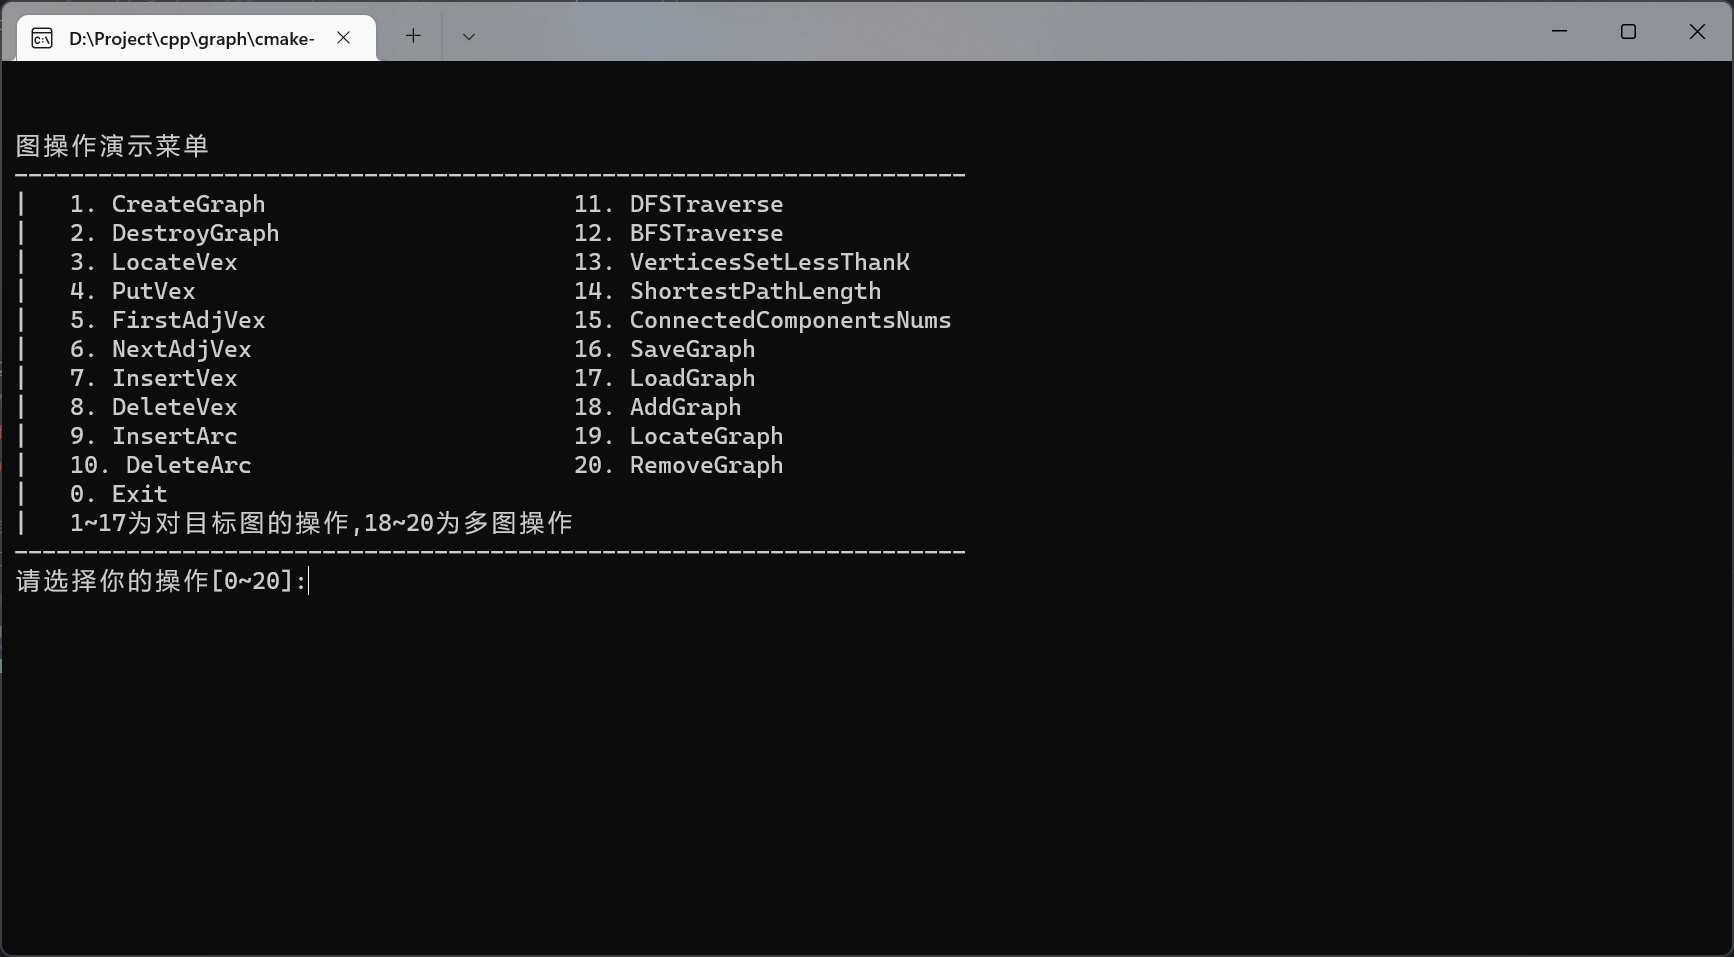
\includegraphics[scale=0.5]{images/p2-1.png}
		\caption{测试界面}
		\label{fig2-1}
	\end{center}
\end{figure}
\subsubsection{测试用例}
测试用例G=(V,E)以及图不存在的情况共两种情况。附有文件123,节点集为V,边集为E。V={v1,v2,v3,v4,v5},E={(v1,v2),(v1,v3),(v2,v3),(v3,v4),(v3,v5),(v4,v5)}。
\newpage
\subsubsection{测试实例}
\begin{enumerate}
	\item CreateGraph测试
	      \begin{table}[htb]
		      \begin{center}
			      \setlength{\tabcolsep}{2.0mm}
			      \caption{CreateGraph测试用例表}
			      \label{t1}
			      \begin{tabular}{|c|c|c|c|}
				      \hline
				      测试用例   & 输入             & 理论结果  & 测试结果  \\
				      \hline
				      \hline
				      未初始化图 & 界面选1,输入样例 & 创建成功! & 创建成功! \\
				      \hline
				      123        & 界面选1          & 图已存在! & 图已存在! \\
				      \hline
			      \end{tabular}
		      \end{center}
	      \end{table}
	      \begin{figure}[htb]
		      \centering
		      \subfloat[未初始化图测试图]{\label{fig2-2}\includegraphics[width=12cm]{images/p2-5.png}}\quad
		      \subfloat[样例测试图]{\label{fig2-3}\includegraphics[width=12cm]{images/p2-6.png}}\\
		      \caption{创建图测试}
	      \end{figure}
	      \newpage
	\item DestroyGraph测试
	      \begin{table}[htb]
		      \begin{center}
			      \setlength{\tabcolsep}{2.0mm}
			      \caption{DestroyGraph测试用例表}
			      \label{t2}
			      \begin{tabular}{|c|c|c|c|}
				      \hline
				      测试用例   & 输入    & 理论结果    & 测试结果    \\
				      \hline
				      \hline
				      未初始化图 & 界面选2 & 图不存在!   & 图不存在!   \\
				      \hline
				      123        & 界面选2 & 图删除成功! & 图删除成功! \\
				      \hline
			      \end{tabular}
		      \end{center}
	      \end{table}
	      \begin{figure}[htb]
		      \centering
		      \subfloat[未初始化图测试图]{\label{fig2-4}\includegraphics[width=12cm]{images/p2-7.png}}\quad
		      \subfloat[测试用例测试图]{\label{fig2-5}\includegraphics[width=12cm]{images/p2-8.png}}\\
		      \caption{销毁图测试}
	      \end{figure}
	      \newpage
	\item LocateVex测试
	      \begin{table}[htb]
		      \begin{center}
			      \setlength{\tabcolsep}{2.0mm}
			      \caption{LocateVex测试用例表}
			      \label{t3}
			      \begin{tabular}{|c|c|c|c|}
				      \hline
				      测试用例   & 输入          & 理论结果               & 测试结果               \\
				      \hline
				      \hline
				      123        & 界面选3,输入2 & 该顶点的位置序号为:1   & 该顶点的位置序号为:1   \\
				      \hline
				      123        & 界面选3,输入9 & 不存在关键字为9的顶点! & 不存在关键字为9的顶点! \\
				      \hline
				      未初始化图 & 界面选3       & 图不存在               & 线图不存在             \\
				      \hline
			      \end{tabular}
		      \end{center}
	      \end{table}
	      \begin{figure}[htb]
		      \centering
		      \subfloat[未初始化表测试图]{\label{fig2-6}\includegraphics[width=7cm]{images/p2-3.png}}\quad
		      \subfloat[错误关键字测试图]{\label{fig2-7}\includegraphics[width=7cm]{images/p2-4.png}}\quad
		      \subfloat[正确关键字测试图]{\label{fig2-8}\includegraphics[width=12cm]{images/p2-2.png}}\\
		      \caption{定位元素测试}
	      \end{figure}
	      \newpage
	\item PutVex测试
	      \begin{table}[htb]
		      \begin{center}
			      \setlength{\tabcolsep}{2.0mm}
			      \caption{PutVex测试用例表}
			      \label{t4}
			      \begin{tabular}{|c|c|c|c|}
				      \hline
				      测试用例   & 输入                  & 理论结果                         & 测试结果      \\
				      \hline
				      \hline
				      123        & 界面选4 输入5 为5 vv5 & \makecell[c]{已将关键字为5的顶点                 \\的内容修改为:5 vv5} & \makecell[c]{已将关键字为5的顶点\\的内容修改为:5 vv5} \\
				      \hline
				      123        & 界面选4 输入4 为5 vv5 & 关键字不唯一!                    & 关键字不唯一! \\
				      \hline
				      未初始化图 & 界面选4               & 图不存在!                        & 图不存在!     \\
				      \hline
			      \end{tabular}
		      \end{center}
	      \end{table}
	      \begin{figure}[htb]
		      \centering
		      \subfloat[未初始化图测试图]{\label{fig2-9}\includegraphics[width=7cm]{images/p2-9.png}}\quad
		      \subfloat[错误关键字测试图]{\label{fig2-10}\includegraphics[width=7cm]{images/p2-11.png}}\quad
		      \subfloat[正确关键字测试图]{\label{fig2-11}\includegraphics[width=12cm]{images/p2-10.png}}\\
		      \caption{节点赋值测试}
	      \end{figure}
	      \newpage
	\item FirstAdjVex测试
	      \begin{table}[htb]
		      \begin{center}
			      \setlength{\tabcolsep}{2.0mm}
			      \caption{FirstAdjVex测试用例表}
			      \label{t5}
			      \begin{tabular}{|c|c|c|c|}
				      \hline
				      测试用例   & 输入          & 理论结果                        & 测试结果                        \\
				      \hline
				      \hline
				      123        & 界面选5,输入1 & 该顶点的第一邻接点的内容为:3 v3 & 该顶点的第一邻接点的内容为:3 v3 \\
				      \hline
				      123        & 界面选5,输入9 & 查找失败!                       & 查找失败!                       \\
				      \hline
				      未初始化图 & 界面选5       & 图不存在                        & 图不存在                        \\
				      \hline
			      \end{tabular}
		      \end{center}
	      \end{table}
	      \begin{figure}[htb]
		      \centering
		      \subfloat[未初始化图测试图]{\label{fig2-12}\includegraphics[width=7cm]{images/p2-14.png}}\quad
		      \subfloat[错误关键字测试图]{\label{fig2-13}\includegraphics[width=7cm]{images/p2-13.png}}\quad
		      \subfloat[正确关键字测试图]{\label{fig2-14}\includegraphics[width=12cm]{images/p2-12.png}}\\
		      \caption{第一邻接点测试}
	      \end{figure}
	      \newpage
	\item NextAdjVex测试
	      \begin{table}[htb]
		      \begin{center}
			      \setlength{\tabcolsep}{2.0mm}
			      \caption{NextAdjVex测试用例表}
			      \label{t6}
			      \begin{tabular}{|c|c|c|c|}
				      \hline
				      测试用例   & 输入                & 理论结果                & 测试结果                \\
				      \hline
				      \hline
				      123        & 界面选6,输入位置3 2 & 查询到的顶点内容为:1 v1 & 查询到的顶点内容为:1 v1 \\
				      \hline
				      123        & 界面选6,输入位置3 9 & 查询失败!               & 查询失败!               \\
				      \hline
				      未初始化图 & 界面选6             & 图不存在                & 图不存在                \\
				      \hline
			      \end{tabular}
		      \end{center}
	      \end{table}
	      \begin{figure}[htb]
		      \centering
		      \subfloat[未初始化图测试图]{\label{fig2-15}\includegraphics[width=7cm]{images/p2-17.png}}\quad
		      \subfloat[错误关键字测试图]{\label{fig2-16}\includegraphics[width=7cm]{images/p2-16.png}}\quad
		      \subfloat[正确关键字测试图]{\label{fig2-17}\includegraphics[width=12cm]{images/p2-15.png}}\\
		      \caption{相对邻接点测试}
	      \end{figure}
	      \newpage
	\item InsertVex测试
	      \begin{table}[htb]
		      \begin{center}
			      \setlength{\tabcolsep}{2.0mm}
			      \caption{InsertVex测试用例表}
			      \label{t7}
			      \begin{tabular}{|c|c|c|c|}
				      \hline
				      测试用例   & 输入                  & 理论结果 & 测试结果 \\
				      \hline
				      \hline
				      123        & 界面选7,输入位置6 v6  & 插入成功 & 插入成功 \\
				      \hline
				      123        & 界面选7,输入位置5 vv5 & 插入失败 & 插入失败 \\
				      \hline
				      未初始化图 & 界面选7               & 图不存在 & 图不存在 \\
				      \hline
			      \end{tabular}
		      \end{center}
	      \end{table}
	      \begin{figure}[htb]
		      \centering
		      \subfloat[未初始化图测试图]{\label{fig2-18}\includegraphics[width=7cm]{images/p2-19.png}}\quad
		      \subfloat[错误关键字测试图]{\label{fig2-19}\includegraphics[width=7cm]{images/p2-18.png}}\quad
		      \subfloat[正确关键字测试图]{\label{fig2-20}\includegraphics[width=12cm]{images/p2-20.png}}\\
		      \caption{插入顶点测试}
	      \end{figure}
	      \newpage
	\item DeleteVex测试
	      \begin{table}[htb]
		      \begin{center}
			      \setlength{\tabcolsep}{2.0mm}
			      \caption{DeleteVex测试用例表}
			      \label{t8}
			      \begin{tabular}{|c|c|c|c|}
				      \hline
				      测试用例   & 输入              & 理论结果 & 测试结果 \\
				      \hline
				      \hline
				      123        & 界面选8,输入位置1 & 删除成功 & 删除成功 \\
				      \hline
				      123        & 界面选8,输入位置6 & 删除失败 & 删除失败 \\
				      \hline
				      未初始化图 & 界面选8           & 图不存在 & 图不存在 \\
				      \hline
			      \end{tabular}
		      \end{center}
	      \end{table}
	      \begin{figure}[htb]
		      \centering
		      \subfloat[未初始化图测试图]{\label{fig2-21}\includegraphics[width=7cm]{images/p2-21.png}}\quad
		      \subfloat[错误关键字测试图]{\label{fig2-22}\includegraphics[width=7cm]{images/p2-22.png}}\quad
		      \subfloat[正确关键字测试图]{\label{fig2-23}\includegraphics[width=12cm]{images/p2-23.png}}\\
		      \caption{删除顶点测试}
	      \end{figure}
	      \newpage
	\item InsertArc测试
	      \begin{table}[htb]
		      \begin{center}
			      \setlength{\tabcolsep}{2.0mm}
			      \caption{InsertArc测试用例表}
			      \label{t9}
			      \begin{tabular}{|c|c|c|c|}
				      \hline
				      测试用例   & 输入                & 理论结果 & 测试结果 \\
				      \hline
				      \hline
				      123        & 界面选9,输入位置1 4 & 插入成功 & 插入成功 \\
				      \hline
				      123        & 界面选9,输入位置1 6 & 插入失败 & 插入失败 \\
				      \hline
				      未初始化图 & 界面选9             & 图不存在 & 图不存在 \\
				      \hline
			      \end{tabular}
		      \end{center}
	      \end{table}
	      \begin{figure}[htb]
		      \centering
		      \subfloat[未初始化图测试图]{\label{fig2-24}\includegraphics[width=7cm]{images/p2-26.png}}\quad
		      \subfloat[错误关键字测试图]{\label{fig2-25}\includegraphics[width=7cm]{images/p2-25.png}}\quad
		      \subfloat[正确关键字测试图]{\label{fig2-26}\includegraphics[width=12cm]{images/p2-24.png}}\\
		      \caption{插入弧测试}
	      \end{figure}
	      \newpage
	\item DeleteArc测试
	      \begin{table}[htb]
		      \begin{center}
			      \setlength{\tabcolsep}{2.0mm}
			      \caption{DeleteArc测试用例表}
			      \label{t10}
			      \begin{tabular}{|c|c|c|c|}
				      \hline
				      测试用例   & 输入                 & 理论结果 & 测试结果 \\
				      \hline
				      \hline
				      123        & 界面选10,输入位置1 2 & 删除成功 & 删除成功 \\
				      \hline
				      123        & 界面选10,输入位置1 6 & 删除失败 & 删除失败 \\
				      \hline
				      未初始化图 & 界面选10             & 图不存在 & 图不存在 \\
				      \hline
			      \end{tabular}
		      \end{center}
	      \end{table}
	      \begin{figure}[htb]
		      \centering
		      \subfloat[未初始化图测试图]{\label{fig2-27}\includegraphics[width=7cm]{images/p2-29.png}}\quad
		      \subfloat[错误关键字测试图]{\label{fig2-28}\includegraphics[width=7cm]{images/p2-28.png}}\quad
		      \subfloat[正确关键字测试图]{\label{fig2-29}\includegraphics[width=12cm]{images/p2-27.png}}\\
		      \caption{插入顶点测试}
	      \end{figure}
	      \newpage
	\item DFSTraverse测试
	      \begin{table}[htb]
		      \begin{center}
			      \setlength{\tabcolsep}{2.0mm}
			      \caption{DFSTraverse测试用例表}
			      \label{t11}
			      \begin{tabular}{|c|c|c|c|}
				      \hline
				      测试用例   & 输入     & 理论结果          & 测试结果 \\
				      \hline
				      \hline
				      List       & 界面选11 & \makecell[c]{1 v1            \\3 v3\\5 v5\\4 v4\\2 v2}   & \makecell[c]{1 v1\\3 v3\\5 v5\\4 v4\\2 v2} \\
				      \hline
				      未初始化图 & 界面选11 & 图不存在          & 图不存在 \\
				      \hline
			      \end{tabular}
		      \end{center}
	      \end{table}
	      \begin{figure}[htb]
		      \centering
		      \subfloat[测试用例测试图]{\label{fig2-30}\includegraphics[width=9cm]{images/p2-30.png}}\quad
		      \subfloat[未初始化图测试图]{\label{fig2-31}\includegraphics[width=9cm]{images/p2-31.png}}\\
		      \caption{DFS测试}
	      \end{figure}
	      \newpage
	\item BFSTraverse测试
	      \begin{table}[htb]
		      \begin{center}
			      \setlength{\tabcolsep}{2.0mm}
			      \caption{BFSTraverse测试用例表}
			      \label{t12}
			      \begin{tabular}{|c|c|c|c|}
				      \hline
				      测试用例   & 输入     & 理论结果           & 测试结果 \\
				      \hline
				      \hline
				      123        & 界面选12 & \makecell[c]{ 1 v1            \\3 v3\\2 v2\\5 v5\\4 v4} & \makecell[c]{ 1 v1\\3 v3\\2 v2\\5 v5\\4 v4} \\
				      \hline
				      未初始化图 & 界面选12 & 图不存在           & 图不存在 \\
				      \hline
			      \end{tabular}
		      \end{center}
	      \end{table}
	      \begin{figure}[htb]
		      \centering
		      \subfloat[测试用例测试图]{\label{fig2-32}\includegraphics[width=9cm]{images/p2-33.png}}\quad
		      \subfloat[未初始化图测试图]{\label{fig2-33}\includegraphics[width=9cm]{images/p2-32.png}}\\
		      \caption{BFS测试}
	      \end{figure}
	      \newpage
	\item VerticesSetLessThanK测试
	      \begin{table}[htb]
		      \begin{center}
			      \setlength{\tabcolsep}{2.0mm}
			      \caption{VerticesSetLessThanK测试用例表}
			      \label{t13}
			      \begin{tabular}{|c|c|c|c|}
				      \hline
				      测试用例   & 输入             & 理论结果  & 测试结果  \\
				      \hline
				      \hline
				      123        & 界面选13,输入1 1 & 3 v3 2 v2 & 3 v3 2 v2 \\
				      \hline
				      未初始化图 & 界面选13         & 图不存在  & 图不存在  \\
				      \hline
			      \end{tabular}
		      \end{center}
	      \end{table}
	      \begin{figure}[htb]
		      \centering
		      \subfloat[测试用例测试图]{\label{fig2-34}\includegraphics[width=12cm]{images/p2-34.png}}\quad
		      \subfloat[未初始化图测试图]{\label{fig2-35}\includegraphics[width=12cm]{images/p2-35.png}}\\
		      \caption{顶点集合测试}
	      \end{figure}
	      \newpage
	\item ShortestPathLength测试
	      \begin{table}[htb]
		      \begin{center}
			      \setlength{\tabcolsep}{2.0mm}
			      \caption{ShortestPathLength测试用例表}
			      \label{t14}
			      \begin{tabular}{|c|c|c|c|}
				      \hline
				      测试用例   & 输入             & 理论结果         & 测试结果         \\
				      \hline
				      \hline
				      123        & 界面选14,输入1 5 & 两者最短距离为:2 & 两者最短距离为:2 \\
				      \hline
				      未初始化图 & 界面选14         & 图不存在         & 图不存在         \\
				      \hline
			      \end{tabular}
		      \end{center}
	      \end{table}
	      \begin{figure}[htb]
		      \centering
		      \subfloat[测试用例测试图]{\label{fig2-36}\includegraphics[width=12cm]{images/p2-36.png}}\quad
		      \subfloat[未初始化图测试图]{\label{fig2-37}\includegraphics[width=12cm]{images/p2-37.png}}\\
		      \caption{最短路径测试}
	      \end{figure}
	      \newpage
	\item ConnectedComponentsNums测试
	      \begin{table}[htb]
		      \begin{center}
			      \setlength{\tabcolsep}{2.0mm}
			      \caption{ConnectedComponentsNums测试用例表}
			      \label{t15}
			      \begin{tabular}{|c|c|c|c|}
				      \hline
				      测试用例       & 输入     & 理论结果          & 测试结果          \\
				      \hline
				      \hline
				      123            & 界面选15 & 图的连通分量为:1  & 图的连通分量为:1  \\
				      \hline
				      未初始化图     & 界面选15 & 图不存在          & 图不存在          \\
				      \hline
				      20个不连通的图 & 界面选15 & 图的连通分量为:20 & 图的连通分量为:20 \\
				      \hline
			      \end{tabular}
		      \end{center}
	      \end{table}
	      \begin{figure}[htb]
		      \centering
		      \subfloat[测试用例测试图]{\label{fig2-38}\includegraphics[width=7cm]{images/p2-39.png}}\quad
		      \subfloat[20个不连通的图]{\label{fig2-39}\includegraphics[width=7cm]{images/p2-38.png}}\quad
		      \subfloat[未初始化图测试图]{\label{fig2-40}\includegraphics[width=12cm]{images/p2-40.png}}\\
		      \caption{连通量测试}
	      \end{figure}
	      \newpage
	\item LocateGraph测试
	      \begin{table}[htb]
		      \begin{center}
			      \setlength{\tabcolsep}{2.0mm}
			      \caption{LocateGraph测试用例表}
			      \label{t16}
			      \begin{tabular}{|c|c|c|c|}
				      \hline
				      测试用例    & 输入             & 理论结果              & 测试结果              \\
				      \hline
				      \hline
				      图1         & 界面选19,输入图1 & 该线性表的位置序号为1 & 该线性表的位置序号为1 \\
				      \hline
				      不存在的图2 & 界面选19,输入图2 & 未找到该图            & 未找到该图            \\
				      \hline
			      \end{tabular}
		      \end{center}
	      \end{table}
	      \begin{figure}[htb]
		      \centering
		      \subfloat[图1测试图]{\label{fig2-41}\includegraphics[width=12cm]{images/p2-41.png}}\quad
		      \subfloat[不存在的表2测试图]{\label{fig2-42}\includegraphics[width=12cm]{images/p2-42.png}}\\
		      \caption{多图定位图测试}
	      \end{figure}
	      \newpage
	\item RemoveGraph测试
	      \begin{table}[htb]
		      \begin{center}
			      \setlength{\tabcolsep}{2.0mm}
			      \caption{RemoveGraph测试用例表}
			      \label{t17}
			      \begin{tabular}{|c|c|c|c|}
				      \hline
				      测试用例    & 输入             & 理论结果          & 测试结果          \\
				      \hline
				      \hline
				      图1         & 界面选20,输入图1 & 移除成功          & 移除成功          \\
				      \hline
				      不存在的图2 & 界面选20,输入图2 & 未找到要移除的图! & 未找到要移除的图! \\
				      \hline
			      \end{tabular}
		      \end{center}
	      \end{table}
	      \begin{figure}[htb]
		      \centering
		      \subfloat[表1测试图]{\label{fig2-43}\includegraphics[width=12cm]{images/p2-43.png}}\quad
		      \subfloat[不存在的表2测试图]{\label{fig2-44}\includegraphics[width=12cm]{images/p2-44.png}}\\
		      \caption{多图移除测试}
	      \end{figure}
	      \newpage
	\item SaveGraph测试
	      \begin{table}[htb]
		      \begin{center}
			      \setlength{\tabcolsep}{2.0mm}
			      \caption{SaveGraph测试用例表}
			      \label{t18}
			      \begin{tabular}{|c|c|c|c|}
				      \hline
				      测试用例   & 输入             & 理论结果     & 测试结果     \\
				      \hline
				      \hline
				      Graph      & 界面选16,输入图1 & 保存成功     & 保存成功     \\
				      \hline
				      未初始化图 & 界面选16,输入123 & 线性表不存在 & 线性表不存在 \\
				      \hline
				      NULL       & 界面选16,输入123 & 线性表为空   & 线性表为空   \\
				      \hline
			      \end{tabular}
		      \end{center}
	      \end{table}
	      \begin{figure}[htb]
		      \centering
		      \subfloat[未初始化图]{\label{fig2-45}\includegraphics[width=7cm]{images/p2-46.png}}\quad
		      \subfloat[Graph]{\label{fig2-46}\includegraphics[width=7cm]{images/p2-45.png}}\quad
		      \subfloat[保存的文件]{\label{fig2-47}\includegraphics[width=12cm]{images/p2-47.png}}\\
		      \caption{保存文件测试}
	      \end{figure}
	      \newpage
	\item LoadGraph测试
	      \begin{table}[htb]
		      \begin{center}
			      \setlength{\tabcolsep}{2.0mm}
			      \caption{LoadGraph测试用例表}
			      \label{t19}
			      \begin{tabular}{|c|c|c|c|}
				      \hline
				      测试用例   & 输入                  & 理论结果 & 测试结果 \\
				      \hline
				      \hline
				      未初始化图 & 界面选17,输入图1      & 读取成功 & 读取成功 \\
				      \hline
				      未初始化图 & 界面选17,输入没有的图 & 读取失败 & 读取失败 \\
				      \hline
				      123        & 界面选17              & 图已存在 & 图已存在 \\
				      \hline
			      \end{tabular}
		      \end{center}
	      \end{table}
	      \begin{figure}[htb]
		      \centering
		      \subfloat[未初始化图]{\label{fig2-48}\includegraphics[width=7cm]{images/p2-48.png}}\quad
		      \subfloat[没有的表]{\label{fig2-49}\includegraphics[width=7cm]{images/p2-49.png}}\quad
		      \subfloat[123]{\label{fig2-50}\includegraphics[width=12cm]{images/p2-50.png}}\\
		      \caption{加载文件测试}
	      \end{figure}
\end{enumerate}
\subsection{实验小结}

实验中要使用较多的指针,而我对指针使用在本次实验中体现出了很多不足之处,比如实验中顶点与连接的顶点之间是以不带头节点的单链表保存,在删除弧的过程中,出现bug调了较长时间才意识到这个问题.

\section{课程的收获和建议}
短暂的数据结构实验课程告一段落,但我十分期待暑假数据结构的课设题目,希望通过本学期的学习,能对接下来的遇到的问题能更快的解决。

\subsection{基于顺序存储结构的线性表实现}

顺序存储结构的线性表实现较为简单,强化了我对于存储结构的基本认识,为接下来的实验打好基础.建议这部分课程的速度可以加快稍稍,来给下面的内容更多的时间加深讲解.

\subsection{基于链式存储结构的线性表实现}

因为第二次实验与第一次实验相比相差不大,仅仅是物理结构发生变化,仅需要做出相应的函数修改即可,因此减轻了一些负担。基本框架不变,从而突出了对单链表的训练,加深了对线性表的概念、基本运算的理解,熟练了线性表的逻辑结构与物理结构的关系,采用了单链表的物理结构,熟练了线性表的基本运算的实现。
在第一次实验的基础上,我对函数进行修改,之后进行测试,最后完善,将注释部分进行完善。

\subsection{基于二叉链表的二叉树实现}

第三次实验的程序中很多函数都可以使用递归来实现,但递归的过程中难免出现很多细小问题,比如说函数何时该返回,返回的不同条件对上一层函数的影响是什么,如何优化函数使递归次数尽量少都是需要注意的地方. 所以本次实验给我的更多的收获在于更能直观的联想到递归的过程了.

\subsection{基于邻接表的图实现}

本次实验我完成的是邻接表形式的无向图,相对于有向图来说简单一些,但这对于我来说还是有些困难。
比如图是一个相互连接的顶点集合,无论使删除顶点还是删除弧,都是牵一发而动全身的,在修改一处时,时常忘记与其相关点的考虑.
实验四花费了我四个实验中最多的时间,但它给我的收获也是最大的,它加深了我对一个程序的概念,每一个函数都要正确的运行才能获得正确的结果.

\newpage
\nocite{*}

\bibliography{Bibs/1}
\setcounter{secnumdepth}{0}
\appendix
\section{代码附录}
\subsection{附录A 基于顺序存储结构线性表实现的源程序}\label{sec:附录a-基于顺序存储结构线性表实现的源程序}
\begin{lstlisting}[caption=顺序表,style=顺序表,title=顺序表]
#include <stdio.h>
#include <stdlib.h>
#include <string.h>
#define TRUE 1
#define FALSE 0
#define OK 1
#define ERROR 0
#define INFEASIBLE -1
#define LISTINITSIZE 100
typedef struct
{  //List(顺序结构)的定义
	int* elem;
	int length;
	int listsize;
} SqList;
typedef struct LISTS
{  //线性表的管理表定义
	struct list
	{
		char name[30];
		SqList L;
	} elem[10];
	int length=0;
	int listsize=10;
} LISTS;
void showmenu()
{
	printf("线性表操作演示菜单\n"
		   "---------------------------------------\n"
		   "1. InitList        7. LocateElem\n"
		   "2. DestroyList     8. PriorElem\n"
		   "3. ClearList       9. NextElem \n"
		   "4. ListEmpty       10. ListInsert\n"
		   "5. ListLength      11. ListDelete\n"
		   "6. GetElem         12. ListTraverse\n"
		   "13. SaveList       14. LoadList\n"
		   "15. SortList       16. MaxSubArray\n"
		   "17. SubArrayNum    18. AddList\n"
		   "19. RemoveList    20. LocateList\n"
		   "0. Exit\n"
		   "1~17为对目标线性表的操作,18~20为多线性表操作\n"
		   "---------------------------------------\n"
	);
}
int InitList(SqList& L)
// 线性表L不存在,构造一个空的线性表,返回OK,否则返回INFEASIBLE。
{
	if (L.elem != NULL) return INFEASIBLE;
	else
	{
		L.elem = (int*)malloc(LISTINITSIZE * sizeof(int));
		L.length = 0;
		L.listsize = LISTINITSIZE;
		return OK;
	}
}
int DestroyList(SqList& L)
// 如果线性表L存在,销毁线性表L,释放数据元素的空间,返回OK,否则返回INFEASIBLE。
{
	if (L.elem)
	{
		free(L.elem);
		L.listsize = 0;
		L.length = 0;
		L.elem = NULL;
		return OK;
	}
	else return INFEASIBLE;
}
int ClearList(SqList& L)
// 如果线性表L存在,删除线性表L中的所有元素,返回OK,否则返回INFEASIBLE。
{
	if (L.elem)
	{
		for (int i = 0; i < L.length; ++i)
		{
			L.elem[i]=0;
		}
		L.length=0;
		return OK;
	}
	else return INFEASIBLE;
}
int ListEmpty(SqList L)
// 如果线性表L存在,判断线性表L是否为空,空就返回TRUE,否则返回FALSE;如果线性表L不存在,返回INFEASIBLE。
{
	if (L.elem)
	{
		if (L.length)return FALSE;
		else return TRUE;
	}
	else return INFEASIBLE;
}
int ListLength(SqList L)
// 如果线性表L存在,返回线性表L的长度,否则返回INFEASIBLE。
{
	if (L.elem)return L.length;
	else return INFEASIBLE;
}
int GetElem(SqList L, int i, int& e)
// 如果线性表L存在,获取线性表L的第i个元素,保存在e中,返回OK;如果i不合法,返回ERROR;如果线性表L不存在,返回INFEASIBLE。
{
	if (L.elem)
	{
		if (i < L.length && i > 0)
		{
			e = L.elem[i - 1];
			return OK;
		}
		else return ERROR;
	}
	else return INFEASIBLE;
}
int LocateElem(SqList L, int e)
// 如果线性表L存在,查找元素e在线性表L中的位置序号并返回该序号;如果e不存在,返回0;当线性表L不存在时,返回INFEASIBLE(即-1)。
{
	if (L.elem)
	{
		for (int i = 0; i < L.length; ++i)
		{
			if (L.elem[i] == e)return i + 1;
		}
		return 0;
	}
	else return INFEASIBLE;
}
int PriorElem(SqList L, int e, int& pre)
// 如果线性表L存在,获取线性表L中元素e的前驱,保存在pre中,返回OK;如果没有前驱,返回ERROR;如果线性表L不存在,返回INFEASIBLE。
{
	if (L.elem)
	{
		for (int i = 0; i < L.length; ++i)
		{
			if (L.elem[i] == e && i > 0)
			{
				pre = L.elem[i - 1];
				return OK;
			}
		}
		return ERROR;
	}
	else return INFEASIBLE;
}
int NextElem(SqList L, int e, int& next)
// 如果线性表L存在,获取线性表L元素e的后继,保存在next中,返回OK;如果没有后继,返回ERROR;如果线性表L不存在,返回INFEASIBLE。
{
	if (L.elem)
	{
		for (int i = 0; i < L.length; ++i)
		{
			if (L.elem[i] == e && i < L.length - 1)
			{
				next = L.elem[i + 1];
				return OK;
			}
		}
		return ERROR;
	}
	else return INFEASIBLE;
}
int ListInsert(SqList& L, int i, int e)
// 如果线性表L存在,将元素e插入到线性表L的第i个元素之前,返回OK;当插入位置不正确时,返回ERROR;如果线性表L不存在,返回INFEASIBLE。
{
	if (L.elem)
	{
		if (i <= 0 || i > L.length + 1)return ERROR;
		if (L.length == L.listsize)
		{
			L.elem[L.length] = *(int*)malloc(sizeof(int));
			L.listsize++;
		}
		for (int j = L.length; j >= i; --j)
		{
			L.elem[j] = L.elem[j - 1];
		}
		L.elem[i - 1] = e;
		L.length++;
		return OK;
	}
	else return 0;
}
int ListDelete(SqList& L, int i, int& e)
// 如果线性表L存在,删除线性表L的第i个元素,并保存在e中,返回OK;当删除位置不正确时,返回ERROR;如果线性表L不存在,返回INFEASIBLE。
{
	if (L.elem)
	{
		if (i <= 0 || i > L.length)return ERROR;
		for (int j = i - 1; j < L.length - 1; ++j)
		{
			if (j == i - 1)
			{
				e = L.elem[j];
			}
			L.elem[j] = L.elem[j + 1];
		}
		L.length--;
		return OK;
	}
	else return INFEASIBLE;
}
int ListTraverse(SqList L)
// 如果线性表L存在,依次显示线性表中的元素,每个元素间空一格,返回OK;如果线性表L不存在,返回INFEASIBLE。
{
	if (L.elem != NULL)
	{
		if (L.length == 0)return -1;
		for (int i = 0; i < L.length; ++i)
		{
			if (i == L.length - 1)
			{
				printf("%d", L.elem[i]);
				break;
			}
			printf("%d ", L.elem[i]);
		}
		return OK;
	}
	else return 0;
}
int SaveList(SqList L, char FileName[])
// 如果线性表L存在,将线性表L的的元素写到FileName文件中,返回OK,否则返回INFEASIBLE。
{
	if (L.elem == NULL)
		return INFEASIBLE;
	FILE* fp;
	if ((fp = fopen(FileName, "w")) == NULL)
	{
		printf("File open error\n ");
		return 0;
	}
	for (int i = 0; i < L.length; ++i)
	{
		fprintf(fp,"%d ",L.elem[i]);
	}
	fclose(fp);
	return OK;
}
int LoadList(SqList& L, char FileName[])
// 如果线性表L不存在,将FileName文件中的数据读入到线性表L中,返回OK,否则返回INFEASIBLE。
{
	if (L.elem != NULL)
		return INFEASIBLE;
	int t;
	L.elem = (int*)malloc(LISTINITSIZE * sizeof(int));
	L.length = 0;
	L.listsize = LISTINITSIZE;
	FILE* fp;
	if ((fp = fopen(FileName, "rb")) == NULL)
	{
		printf("File open error\n ");
		return 0;
	}
	while (!feof(fp))
	{
		fscanf(fp, "%d", &t);
		L.elem[L.length++] = t;
	}
	fclose(fp);
	return OK;
}
int AddList(LISTS& Lists, char ListName[])
// 只需要在Lists中增加一个名称为ListName的空线性表,线性表数据又后台测试程序插入。
{
	for (int i = 0; i < Lists.length; ++i)
	{
		if (strcmp(Lists.elem[i].name, ListName) == 0)
			return -1;
	}
	Lists.elem[Lists.length].L.length = 0;
	Lists.elem[Lists.length].L.listsize = LISTINITSIZE;
	Lists.elem[Lists.length].L.elem = NULL;
	strcpy(Lists.elem[Lists.length].name, ListName);
	Lists.length++;
	return OK;
}

int RemoveList(LISTS& Lists, char ListName[])
// Lists中删除一个名称为ListName的线性表
{
	int i;
	for (i = 0; i < Lists.length; ++i)
	{
		if (strcmp(ListName, Lists.elem[i].name) == 0)
		{
			for (int k = i; k < Lists.length - 1; ++k)
			{
				Lists.elem[k] = Lists.elem[k + 1];
			}
			Lists.length--;
			return OK;
		}
	}
	return 0;
}

int LocateList(LISTS Lists, char ListName[])
// 在Lists中查找一个名称为ListName的线性表,成功返回逻辑序号,否则返回0
{
	for (int i = 0; i < Lists.length; ++i)
	{
		if(strcmp(Lists.elem[i].name, ListName)==0)
			return i;
	}
	return -1;
}
int SortList(SqList& L)
{
	if (L.elem == NULL || L.length == 0)
		return INFEASIBLE;
	for (int j = L.length - 1; j >= 1; j--)
	{
		for (int i = 0; i < j; i++)
		{
			if (L.elem[i] > L.elem[i + 1])
			{
				int t = L.elem[i];
				L.elem[i] = L.elem[i + 1];
				L.elem[i + 1] = t;
			}
		}
	}
	return OK;
}
int MaxSubArray(SqList L, int& e)
{
	if (L.elem == NULL || L.length == 0)
		return INFEASIBLE;
	int flag = 0;
	for (int i = 0; i < L.length; i++)
	{
		if (L.elem[i] > 0)
		{
			flag = 1;
			break;
		}
	}
	if (flag == 0)
	{
		int max = L.elem[0];
		for (int i = 0; i < L.length; i++)
			if (L.elem[i] > max) max = L.elem[i];
		e = max;
		return OK;
	}
	else
	{
		int max = 0, now = 0;
		for (int i = 0; i < L.length; i++)
		{
			now += L.elem[i];
			max = max > now ? max : now;
			if (now < 0) now = 0;
		}
		e = max;
		return OK;
	}
}
int SubArrayNum(SqList L, int k)
{
	if (L.elem == NULL) return -1;
	int num = 0;
	int i, j;
	for (i = 0; i < L.length; i++)
	{
		int sum = 0;
		for (j = i; j < L.length; j++)
		{
			sum += L.elem[j];
			if (sum == k)
			{
				num++;
			}
		}
	}
	return num;
}
int function(SqList& L, int op)
{
	int i, e, t, pre, next;
	char filename[30];
	switch (op)
	{
	case 1:
		if (InitList(L) == OK) printf("线性表创建成功!\n");
		else printf("线性表创建失败!\n");
		getchar();
		system("pause");
		break;
	case 2:
		if (DestroyList(L) == OK) printf("线性表销毁成功!\n");
		else printf("线性表销毁失败!\n");
		getchar();
		system("pause");
		break;
	case 3:
		if (ClearList(L) == OK) printf("线性表删除成功!\n");
		else printf("线性表删除失败!\n");
		getchar();
		system("pause");
		break;
	case 4:
		if (ListEmpty(L) == TRUE) printf("线性表是空的!\n");
		else if (ListEmpty(L) == FALSE) printf("线性表不是空的!\n");
		else printf("线性表不存在\n");
		getchar();
		system("pause");
		break;
	case 5:
		if (ListLength(L) == INFEASIBLE)
			printf("线性表不存在!\n");
		else printf("线性表的长度是%d!\n", ListLength(L));
		getchar();
		system("pause");
		break;
	case 6:
		if (ListEmpty(L) == TRUE) printf("线性表为空\n");
		else
		{
			printf("\n----请输入查找元素的序号!\n");
			scanf("%d", &i);
			if (GetElem(L, i, e) == OK)
				printf("第%d个元素是%d!\n", i, e);
			else printf("不存在第%d个元素!\n", i);
		}
		getchar();
		system("pause");
		break;
	case 7:
		if (ListEmpty(L) == TRUE) printf("线性表为空\n");
		else
		{
			printf("\n----请输入所需查找的元素!\n");
			scanf("%d", &e);
			t = LocateElem(L, e);
			if (t == INFEASIBLE || t == ERROR)
				printf("该元素不存在!\n");
			else printf("这个元素是第%d个!\n", t);
		}
		getchar();
		system("pause");
		break;
	case 8:
		if (ListEmpty(L) == TRUE) printf("线性表为空\n");
		else
		{
			printf("\n----请输入目标元素!\n");
			scanf("%d", &e);
			if (PriorElem(L, e, pre) != OK)
				printf("该元素不存在前驱元素!\n");
			else printf("该元素的前驱元素是%d!\n", pre);
		}
		getchar();
		system("pause");
		break;
	case 9:
		if (ListEmpty(L) == TRUE) printf("线性表为空\n");
		else
		{
			printf("\n----请输入目标元素!\n");
			scanf("%d", &e);
			if (NextElem(L, e, next) != OK)
				printf("该元素不存在后继元素!\n");
			else printf("该元素的后继元素是%d!\n", next);
		}
		getchar();
		system("pause");
		break;
	case 10:
		if (ListEmpty(L) == TRUE) printf("线性表为空\n");
		else
		{
			printf("\n----请输入插入位置和所需插入的元素!\n");
			scanf("%d %d", &i, &e);
			if (ListInsert(L, i, e) == OK)
				printf("插入成功!\n");
			else printf("插入失败!\n");
		}
		getchar();
		system("pause");
		break;
	case 11:
		if (ListEmpty(L) == TRUE) printf("线性表为空\n");
		else
		{
			printf("\n----请输入所需删除元素的位置!\n");
			scanf("%d", &i);
			if (ListDelete(L, i, e) == OK)
				printf("元素删除成功,该元素是%d!\n", e);
			else printf("元素删除失败!\n");
		}
		getchar();
		system("pause");
		break;
	case 12:
		if (ListLength(L) == -1)
		{
			printf("线性表为空!");
			getchar();
			system("pause");
			break;
		}
		if (!ListTraverse(L)) printf("线性表不存在!\n");
		else printf("\n元素遍历完成!\n");
		getchar();
		system("pause");
		break;
	case 13:
		if (ListEmpty(L) == TRUE) printf("线性表为空\n");
		else
		{
			printf("\n----请输入文件名!\n");
			scanf("%s", filename);
			if (SaveList(L, filename) == OK) printf("文件写入成功!\n");
			else printf("文件写入失败!\n");
		}
		getchar();
		system("pause");
		break;
	case 14:
		if (ListEmpty(L) != TRUE) printf("线性表不为空\n");
		else
		{
			printf("\n----请输入文件名!\n");
			scanf("%s", filename);
			if (LoadList(L, filename) == OK) printf("文件读取成功!\n");
			else printf("文件读取失败!\n");
		}
		getchar();
		system("pause");
		break;
	case 15:
		if (ListEmpty(L) == TRUE) printf("线性表为空\n");
		else
		{
			if (SortList(L) == OK) printf("线性表排序完成!\n");
			else printf("线性表不存在或没有元素!\n");
		}
		getchar();
		system("pause");
		break;
	case 16:
		if (MaxSubArray(L, e) == OK) printf("线性表的最大子数组和是%d!\n", e);
		else printf("线性表不存在!\n");
		getchar();
		system("pause");
		break;
	case 17:
		if (ListEmpty(L) == TRUE) printf("线性表为空\n");
		else
		{
			printf("----请输入目标数字\n");
			scanf("%d", &e);
			t = SubArrayNum(L, e);
			if (t == -1) printf("线性表不存在!\n");
			else printf("子数组总共有%d个!\n", t);
		}
		getchar();
		system("pause");
		break;
	case 0:
		return 0;
	}
	system("cls");
	showmenu();
	printf("请继续输入你要对此线性表执行的操作[1~17],按0退出!\n");
	scanf("%d", &i);
	return i;
};

#include "def.h"
#include "stu.h"

int main()
{
	SqList L;
	int op = 1;
	L.elem = NULL;
	int i, e, t, pre, next, num;
	char filename[30], listname[30];
	LISTS lists;
	lists.length = 0;
	lists.listsize = 10;
	while (op)
	{
		system("cls");
		printf("\n\n");
		showmenu();
		printf("请输入你的操作[0~20]:");
		scanf("%d", &op);
		switch (op)
		{
		case 1:
			if (InitList(L) == OK) printf("线性表创建成功!\n");
			else printf("线性表创建失败!\n");
			getchar();
			system("pause");
			break;
		case 2:
			if (DestroyList(L) == OK) printf("线性表销毁成功!\n");
			else printf("线性表销毁失败!\n");
			getchar();
			system("pause");
			break;
		case 3:
			if (ClearList(L) == OK) printf("线性表删除成功!\n");
			else printf("线性表删除失败!\n");
			getchar();
			system("pause");
			break;
		case 4:
			if (ListEmpty(L) == TRUE) printf("线性表是空的!\n");
			else if (ListEmpty(L) == FALSE) printf("线性表不是空的!\n");
			else printf("线性表不存在\n");
			getchar();
			system("pause");
			break;
		case 5:
			if (ListLength(L) == INFEASIBLE)
				printf("线性表不存在!\n");
			else printf("线性表的长度是%d!\n", ListLength(L));
			getchar();
			system("pause");
			break;
		case 6:
			if (ListEmpty(L) == TRUE) printf("线性表为空\n");
			else
			{
				printf("\n----请输入查找元素的序号!\n");
				scanf("%d", &i);
				if (GetElem(L, i, e) == OK)
					printf("第%d个元素是%d!\n", i, e);
				else printf("不存在第%d个元素!\n", i);
			}
			getchar();
			system("pause");
			break;
		case 7:
			if (ListEmpty(L) == TRUE) printf("线性表为空\n");
			else
			{
				printf("\n----请输入所需查找的元素!\n");
				scanf("%d", &e);
				t = LocateElem(L, e);
				if (t == INFEASIBLE || t == ERROR)
					printf("该元素不存在!\n");
				else printf("这个元素是第%d个!\n", t);
			}
			getchar();
			system("pause");
			break;
		case 8:
			if (ListEmpty(L) == TRUE) printf("线性表为空\n");
			else
			{
				printf("\n----请输入目标元素!\n");
				scanf("%d", &e);
				if (PriorElem(L, e, pre) != OK)
					printf("该元素不存在前驱元素!\n");
				else printf("该元素的前驱元素是%d!\n", pre);
			}
			getchar();
			system("pause");
			break;
		case 9:
			if (ListEmpty(L) == TRUE) printf("线性表为空\n");
			else
			{
				printf("\n----请输入目标元素!\n");
				scanf("%d", &e);
				if (NextElem(L, e, next) != OK)
					printf("该元素不存在后继元素!\n");
				else printf("该元素的后继元素是%d!\n", next);
			}
			getchar();
			system("pause");
			break;
		case 10:
			if (ListEmpty(L) == TRUE) printf("线性表为空\n");
			else
			{
				printf("\n----请输入插入位置和所需插入的元素!\n");
				scanf("%d %d", &i, &e);
				if (ListInsert(L, i, e) == OK)
					printf("插入成功!\n");
				else printf("插入失败!\n");
			}
			getchar();
			system("pause");
			break;
		case 11:
			if (ListEmpty(L) == TRUE) printf("线性表为空\n");
			else
			{
				printf("\n----请输入所需删除元素的位置!\n");
				scanf("%d", &i);
				if (ListDelete(L, i, e) == OK)
					printf("元素删除成功,该元素是%d!\n", e);
				else printf("元素删除失败!\n");
			}
			getchar();
			system("pause");
			break;
		case 12:
			if (ListLength(L) == -1)
			{
				printf("线性表为空!");
				getchar();
				system("pause");
				break;
			}
			if (!ListTraverse(L)) printf("线性表不存在!\n");
			else printf("\n元素遍历完成!\n");
			getchar();
			system("pause");
			break;
		case 13:
			if (ListEmpty(L) == TRUE) printf("线性表为空\n");
			else
			{
				printf("\n----请输入文件名!\n");
				scanf("%s", filename);
				if (SaveList(L, filename) == OK) printf("文件写入成功!\n");
				else printf("文件写入失败!\n");
			}
			getchar();
			system("pause");
			break;
		case 14:
			if (ListEmpty(L) != TRUE) printf("线性表不为空\n");
			else
			{
				printf("\n----请输入文件名!\n");
				scanf("%s", filename);
				if (LoadList(L, filename) == OK) printf("文件读取成功!\n");
				else printf("文件读取失败!\n");
			}
			getchar();
			system("pause");
			break;
		case 15:
			if (ListEmpty(L) == TRUE) printf("线性表为空\n");
			else
			{
				if (SortList(L) == OK) printf("线性表排序完成!\n");
				else printf("线性表不存在或没有元素!\n");
			}
			getchar();
			system("pause");
			break;
		case 16:
			if (MaxSubArray(L, e) == OK) printf("线性表的最大子数组和是%d!\n", e);
			else printf("线性表不存在!\n");
			getchar();
			system("pause");
			break;
		case 17:
			if (ListEmpty(L) == TRUE) printf("线性表为空\n");
			else
			{
				printf("----请输入目标数字\n");
				scanf("%d", &e);
				t = SubArrayNum(L, e);
				if (t == -1) printf("线性表不存在!\n");
				else printf("子数组总共有%d个!\n", t);
			}
			getchar();
			system("pause");
			break;
		case 18:
			printf("\n----请输入所需添加的列表名!\n");
			scanf("%s", listname);
			if (AddList(lists, listname) == OK) printf("新建线性表成功!\n");
			else printf("新建线性表失败!\n");
			getchar();
			system("pause");
			break;
		case 19:
			printf("\n----请输入所需删除的列表名!\n");
			scanf("%s", listname);
			if (RemoveList(lists, listname) == OK) printf("删除线性表成功!\n");
			else printf("删除线性表失败!\n");
			getchar();
			system("pause");
			break;
		case 20:
			printf("\n----请输入所需查找的列表名!\n");
			scanf("%s", listname);
			if ((num = LocateList(lists, listname) != 0))
			{
				printf("该列表的逻辑序号为%d\n", num+1);
				printf("请输入你要对此线性表执行的操作[1~17],按0退出!\n");
				scanf("%d", &op);
				while (op)
				{
					system("cls");
					showmenu();
					op = function(lists.elem[LocateList(lists, listname) - 1].L, op);
				}
				op = 1;
			}
			else
			{
				printf("未找到该线性表\n");
				getchar();
				system("pause");
				break;
			}
			getchar();
			system("pause");
			break;
		default:
			break;
		}
	}
	DestroyList(L);
	printf("欢迎下次再使用本系统!\n");
}
\end{lstlisting}
\newpage
\subsection{附录B 基于链式存储结构线性表实现的源程序}\label{sec:附录b-基于链式存储结构线性表实现的源程序}
\begin{lstlisting}[caption=线性表,style=线性表,title=线性表]
#include "stdio.h"
#include "stdlib.h"
#include <string.h>

#define OK 1
#define ERROR 0

typedef int status;
typedef int ElemType; //数据元素类型定义
typedef struct LNode
{  //单链表(链式结构)结点的定义
	ElemType data;
	struct LNode* next;
} LNode, * LinkList;
typedef struct LISTS
{
	struct L
	{
		char name[30]{};
		LinkList L = NULL;
	} elem[10];
	int length = 0;
	int listsize = 10;
} LISTS;
void showmenu()
{
	printf("线性表操作演示菜单\n"
		   "---------------------------------------\n"
		   "1. InitList        7. LocateElem\n"
		   "2. DestroyList     8. PriorElem\n"
		   "3. ClearList       9. NextElem \n"
		   "4. ListEmpty       10. ListInsert\n"
		   "5. ListLength      11. ListDelete\n"
		   "6. GetElem         12. ListTraverse\n"
		   "13. ReverseList    14. RemoveNthFromEnd\n"
		   "15. SortList       16. SaveList\n"
		   "17. LoadList       18. AddList\n"
		   "19. LocateList     20. RemoveList\n"
		   "21. ListNumsInsert 0. Exit\n"
		   "1~17为对目标线性表的操作,18~20为多线性表操作\n"
		   "21为空表的多数据插入\n"
		   "---------------------------------------\n"
	);
}
status InitList(LinkList& L)
// 线性表L不存在,构造一个空的线性表,返回OK,否则返回INFEASIBLE。
{
	if (L == NULL)
	{
		L = (LinkList)malloc(sizeof(LNode));
		L->next = NULL;
		return OK;
	}
	return -1;
}

status DestroyList(LinkList& L)
// 如果线性表L存在,销毁线性表L,释放数据元素的空间,返回OK,否则返回INFEASIBLE。
{
	if (L == NULL) return -1;
	LinkList t, p;
	p = L;
	while (p->next)
	{
		t = p;
		p = p->next;
		free(t);
	}
	free(p);
	L=NULL;
	return OK;
}

status ClearList(LinkList& L)
// 如果线性表L存在,删除线性表L中的所有元素,返回OK,否则返回INFEASIBLE。
{
	if (!L) return -1;
	else if (!L->next) return 0;
	LinkList p, t;
	p = L->next;
	while (p && p->next)
	{
		t = p;
		p = p->next;
		free(t);
	}
	L->next = NULL;
	return OK;
}

status ListEmpty(LinkList L)
// 如果线性表L存在,判断线性表L是否为空,空就返回TRUE,否则返回FALSE;如果线性表L不存在,返回INFEASIBLE。
{
	if (L == NULL) return -1;
	if (L->next) return 0;
	else return 1;
}

int ListLength(LinkList L)
// 如果线性表L存在,返回线性表L的长度,否则返回INFEASIBLE。
{
	if (L == NULL) return -1;
	if (L->next == NULL) return 0;
	int i = 1;
	LinkList p;
	for (p = L->next; p->next; i++)
	{
		p = p->next;
	}
	return i;
}

status GetElem(LinkList L, int i, ElemType& e)
// 如果线性表L存在,获取线性表L的第i个元素,保存在e中,返回OK;如果i不合法,返回ERROR;如果线性表L不存在,返回INFEASIBLE。
{
	if (!L) return -1;
	int p = 1;
	LinkList t = L->next;
	while (t && p != i)
	{
		t = t->next;
		p++;
	}
	if (!t) return ERROR;
	else e = t->data;
	return OK;
}

status LocateElem(LinkList L, ElemType e)
// 如果线性表L存在,查找元素e在线性表L中的位置序号;如果e不存在,返回ERROR;当线性表L不存在时,返回INFEASIBLE。
{
	if (L == NULL) return -1;
	LinkList t;
	int p = 1;
	t = L->next;
	while (t && t->data != e)
	{
		t = t->next;
		p++;
	}
	if (!t) return ERROR;
	return p;
}

status PriorElem(LinkList L, ElemType e, ElemType& pre)
// 如果线性表L存在,获取线性表L中元素e的前驱,保存在pre中,返回OK;如果没有前驱,返回ERROR;如果线性表L不存在,返回INFEASIBLE。
{
	LinkList c, p;
	if (!L) return -1;
	if(!LocateElem(L, e))return -2;
	c = L->next;
	p = L;
	while (c && c->data != e)
	{
		c = c->next;
		p = p->next;
	}
	if (!c || p == L) return ERROR;
	pre = p->data;
	return OK;
}

status NextElem(LinkList L, ElemType e, ElemType& next)
// 如果线性表L存在,获取线性表L元素e的后继,保存在next中,返回OK;如果没有后继,返回ERROR;如果线性表L不存在,返回INFEASIBLE。
{
	LinkList c;
	if (!L) return -1;
	if(!LocateElem(L, e))return -2;
	c = L->next;
	while (c && c->data != e)
	{
		c = c->next;
	}
	if (!c || !c->next) return ERROR;
	next = c->next->data;
	return OK;
}

status ListInsert(LinkList& L, int i, ElemType e)
// 如果线性表L存在,将元素e插入到线性表L的第i个元素之前,返回OK;当插入位置不正确时,返回ERROR;如果线性表L不存在,返回INFEASIBLE。
{
	if (!L) return -1;
	if (i == 0) return ERROR;
	LinkList p, c;
	c = L->next;
	p = L;
	int k = 1;
	while (k != i && c)
	{
		p = c;
		c = c->next;
		k++;
	}
	if (k != i) return ERROR;
	LinkList t;
	t = (LinkList)malloc(sizeof(LinkList));
	t->next = c;
	t->data = e;
	p->next = t;
	return OK;
}

status ListDelete(LinkList& L, int i, ElemType& e)
// 如果线性表L存在,删除线性表L的第i个元素,并保存在e中,返回OK;当删除位置不正确时,返回ERROR;如果线性表L不存在,返回INFEASIBLE。
{
	if (!L) return -1;
	if (i == 0) return ERROR;
	int k = 1;
	LinkList c, p;
	c = L->next;
	p = L;
	while (k != i && c)
	{
		p = c;
		c = c->next;
		k++;
	}
	if (k != i || !c) return ERROR;
	e = c->data;
	p->next = c->next;
	free(c);
	return OK;
}

status ListTraverse(LinkList L)
// 如果线性表L存在,依次显示线性表中的元素,每个元素间空一格,返回OK;如果线性表L不存在,返回INFEASIBLE。
{
	if (!L) return -1;
	LinkList c;
	c = L->next;
	if (!c) return ERROR;
	while (c->next)
	{
		printf("%d ", c->data);
		c = c->next;
	}
	printf("%d", c->data);
	return OK;
}

status SaveList(LinkList L, char FileName[])
// 如果线性表L存在,将线性表L的的元素写到FileName文件中,返回OK,否则返回INFEASIBLE。
{
	if (!L) return -1;
	if(!L->next)return 0;
	FILE* fp;
	if ((fp = fopen(FileName, "w")) == NULL)return -1;
	L = L->next;
	while (L)
	{
		fprintf(fp, "%d ", L->data);
		L = L->next;
	}
	fclose(fp);
	return 1;
}

status LoadList(LinkList& L, char FileName[])
// 如果线性表L不存在,将FileName文件中的数据读入到线性表L中,返回OK,否则返回INFEASIBLE。
{
	FILE* fp;
	if ((fp = fopen(FileName, "r")) == NULL)return -1;
	if (L) return 0;
	L = (LinkList)malloc(sizeof(LNode));
	auto* p = (LNode*)malloc(sizeof(LNode));
	LNode* t;
	t = NULL;
	t = L;
	while (fscanf(fp, "%d", &p->data) != EOF)
	{
		t->next = p;
		t = p;
		p = (LNode*)malloc(sizeof(LNode));
	}
	p = NULL;
	t->next = NULL;
	fclose(fp);
	return 1;
}

status reverseList(LinkList& L)
{
//	链表翻转
	LNode* c, * p;
	if (!L) return -1;//不存在
	if (!L->next) return 0;//空
	if (!L->next->next) return 1;
	c=L->next;
	L->next = NULL;
	while (c){
		p=c->next;
		c->next=L->next;
		L->next=c;
		c=p;
	}
	return 1;
}

status RemoveNthFromEnd(LinkList& L, int n)
{
//	移除倒数第n个元素
	if (!L) return -1;
	if (!L->next) return -1;
	LNode* fast, * slow,*temp;
	fast = slow = L;
	int i;
	for (i = 0; i <= n && fast != NULL; i++)
	{
		fast = fast->next;
	}
	if (i <=n)return 0;
	while (fast)
	{
		slow = slow->next;
		fast = fast->next;
	}
	temp=slow->next;
	slow->next = slow->next->next;
	free(temp);
	return 1;
}

status sortList(LinkList& L)
{
//	链表排序---冒泡排序
	if (!L) return -1;
	if (!L->next) return 0;
	LinkList p, q;
	for (p = L->next; p->next; p = p->next)
	{
		for (q = p; q->next; q = q->next)
		{
			if (p->data > q->next->data)
			{
				int tmp = p->data;
				p->data = q->next->data;
				q->next->data = tmp;
			}
		}
	}
	return 1;
}

int LocateLinkList(LISTS L, char listName[])
{
//	定位链表
	int i;
	for (i = 0; i < L.length; i++)
		if (strcmp(listName, L.elem[i].name) == 0)
			return i;
	return -1;
}

status AddList(LISTS& Lists, char ListName[])
// 只需要在Lists中增加一个名称为ListName的空线性表,线性表数据又后台测试程序插入。
{
	for (int i = 0; i < Lists.length; ++i)
	{
		if (strcmp(ListName, Lists.elem[i].name) == 0)
			return 0;
	}
	InitList(Lists.elem[Lists.length].L);
	strcpy(Lists.elem[Lists.length].name, ListName);
	Lists.length++;
	return OK;
}

status RemoveList(LISTS& lists, char listname[])
{
	int flag = 0;
	for (int i = 0; i < lists.length; ++i)
	{
		if (strcmp(listname, lists.elem[i].name) == 0)
		{
			for (int j = i; j < lists.length; ++j)
			{
				lists.elem[j] = lists.elem[j + 1];
			}
			flag = 1;
		}
	}
	if (flag == 0)return 0;
	lists.length--;
	return OK;
}

int function(LinkList& L, int op)
{
	int e, i, pos, pre, next;
	int temp = 1, num;
	char c;
	char* Filename = (char*)malloc(sizeof(char) * 100);
	switch (op)
	{
	case 1:
		if (InitList(L) == OK) printf("线性表创建成功!\n");
		else printf("线性表创建失败!\n");
		getchar();
		system("pause");
		break;
	case 2:
		if (DestroyList(L) == 1) printf("线性表删除成功");
		else printf("线性表删除失败");
		getchar();
		system("pause");
		break;
	case 3:
		pos = ClearList(L);
		if (pos == 1) printf("线性表清空");
		else if (pos == 0) printf("线性表为空");
		else printf("线性表不存在");
		getchar();
		system("pause");
		break;
	case 4:
		pos = ListEmpty(L);
		if (pos == 1) printf("线性表为空");
		if (!pos)printf("线性表不为空");
		if (pos == -1) printf("线性表不存在");
		getchar();
		system("pause");
		break;
	case 5:
		pos = ListLength(L);
		if (pos == -1) printf("线性表不存在");
		else if (pos) printf("线性表长%d", pos);
		else printf("线性表为空");
		getchar();
		system("pause");
		break;
	case 6:
		printf("请输入你要获取的元素的位置:");
		scanf("%d", &i);
		pos = GetElem(L, i, e);
		if (pos == -1) printf("线性表不存在");
		if (pos) printf("第%d个元素为%d", i, e);
		else printf("不存在第%d个元素", i);
		getchar();
		system("pause");
		break;
	case 7:
		printf("请输入你要获取的位置的元素:");
		scanf("%d", &e);
		pos = LocateElem(L, e);
		if (pos == -1) printf("线性表不存在");
		else if (pos == 0) printf("不存在为%d的元素", e);
		else printf("元素%d位于第%d个", e, pos);
		getchar();
		system("pause");
		break;
	case 8:
		printf("请输入你要获取前驱元素的位置:");
		scanf("%d", &e);
		pos = PriorElem(L, e, pre);
		if (pos == -1) printf("线性表不存在");
		else if (pos == 0) printf("不存在元素:%d", e);
		else printf("元素%d的前继元素为:%d", e, pre);
		getchar();
		system("pause");
		break;
	case 9:
		printf("请输入你要获取后驱元素的位置:");
		scanf("%d", &e);
		pos = NextElem(L, e, next);
		if (pos == -1) printf("线性表不存在");
		else if (pos == 0) printf("不存在%d的后继", e);
		else printf("%d的后继是%d", e, next);
		getchar();
		system("pause");
		break;
	case 10:
		printf("请输入你要插入位置及元素值:");
		scanf("%d %d", &i, &e);
		pos = ListInsert(L, i, e);
		if (pos == -1) printf("线性表不存在");
		else if (pos == 0) printf("插入失败");
		else printf("插入成功");
		getchar();
		system("pause");
		break;
	case 11:
		printf("请输入你要删除取的元素的位置:");
		scanf("%d", &i);
		pos = ListDelete(L, i, e);
		if (pos == -1) printf("线性表不存在");
		else if (pos == 0) printf("删除失败");
		else printf("删除成功,该元素值为%d", e);
		getchar();
		system("pause");
		break;
	case 12:
		pos = ListTraverse(L);
		if (pos == -1) printf("线性表不存在");
		else if (pos == 0) printf("线性表为空");
		else printf("遍历完成!\n");
		getchar();
		system("pause");
		break;
	case 13:
		pos = reverseList(L);
		if (pos == -1) printf("线性表不存在");
		else if (!pos) printf("线性表为空");
		else printf("线性表已翻转!");
		getchar();
		system("pause");
		break;
	case 14:
		printf("请输入你要删除的倒数第n个元素的位置:");
		scanf("%d", &i);
		pos = RemoveNthFromEnd(L, i);
		if (pos == -1) printf("线性表不存在");
		else if (!pos) printf("删除失败");
		else printf("删除成功");
		getchar();
		system("pause");
		break;
	case 15:
		pos = sortList(L);
		if (pos == -1) printf("线性表不存在");
		else if (!pos) printf("线性表为空");
		else printf("排序成功");
		getchar();
		system("pause");
		break;
	case 16:
		printf("请输入你要保存的文件名:");
		scanf("%s", Filename);
		if (SaveList(L, Filename) == 1) printf("保存成功");
		else printf("写入失败");
		getchar();
		system("pause");
		break;
	case 17:
		printf("请输入你要读取的文件名:");
		scanf("%s", Filename);
		if (LoadList(L, Filename) == 1) printf("读取成功");
		else printf("读取失败");
		getchar();
		system("pause");
		break;
	case 21:
		if (ListEmpty(L) == 1)
		{
			printf("请输入你要给空表添加的连续数据:\n以'.'为结束\n");
			scanf("%d%c", &num, &c);
			while (c != '.')
			{
				ListInsert(L, temp++, num);
				scanf("%d%c", &num, &c);
			}
			getchar();
		}
		else printf("该表不为空!\n");
		system("pause");
		break;
	default:
		break;
	}
	system("cls");
	showmenu();
	printf("请继续输入你要对此线性表执行的操作[1~17],按0退出!\n");
	scanf("%d", &i);
	return i;
}

#include "def.h"
#include "stu.h"

int main()
{
	SqList L;
	int op = 1;
	L.elem = NULL;
	int i, e, t, pre, next, num;
	char filename[30], listname[30];
	LISTS lists;
	lists.length = 0;
	lists.listsize = 10;
	while (op)
	{
		system("cls");
		printf("\n\n");
		showmenu();
		printf("请输入你的操作[0~20]:");
		scanf("%d", &op);
		switch (op)
		{
		case 1:
			if (InitList(L) == OK) printf("线性表创建成功!\n");
			else printf("线性表创建失败!\n");
			getchar();
			system("pause");
			break;
		case 2:
			if (DestroyList(L) == OK) printf("线性表销毁成功!\n");
			else printf("线性表销毁失败!\n");
			getchar();
			system("pause");
			break;
		case 3:
			if (ClearList(L) == OK) printf("线性表删除成功!\n");
			else printf("线性表删除失败!\n");
			getchar();
			system("pause");
			break;
		case 4:
			if (ListEmpty(L) == TRUE) printf("线性表是空的!\n");
			else if (ListEmpty(L) == FALSE) printf("线性表不是空的!\n");
			else printf("线性表不存在\n");
			getchar();
			system("pause");
			break;
		case 5:
			if (ListLength(L) == INFEASIBLE)
				printf("线性表不存在!\n");
			else printf("线性表的长度是%d!\n", ListLength(L));
			getchar();
			system("pause");
			break;
		case 6:
			if (ListEmpty(L) == TRUE) printf("线性表为空\n");
			else
			{
				printf("\n----请输入查找元素的序号!\n");
				scanf("%d", &i);
				if (GetElem(L, i, e) == OK)
					printf("第%d个元素是%d!\n", i, e);
				else printf("不存在第%d个元素!\n", i);
			}
			getchar();
			system("pause");
			break;
		case 7:
			if (ListEmpty(L) == TRUE) printf("线性表为空\n");
			else
			{
				printf("\n----请输入所需查找的元素!\n");
				scanf("%d", &e);
				t = LocateElem(L, e);
				if (t == INFEASIBLE || t == ERROR)
					printf("该元素不存在!\n");
				else printf("这个元素是第%d个!\n", t);
			}
			getchar();
			system("pause");
			break;
		case 8:
			if (ListEmpty(L) == TRUE) printf("线性表为空\n");
			else
			{
				printf("\n----请输入目标元素!\n");
				scanf("%d", &e);
				if (PriorElem(L, e, pre) != OK)
					printf("该元素不存在前驱元素!\n");
				else printf("该元素的前驱元素是%d!\n", pre);
			}
			getchar();
			system("pause");
			break;
		case 9:
			if (ListEmpty(L) == TRUE) printf("线性表为空\n");
			else
			{
				printf("\n----请输入目标元素!\n");
				scanf("%d", &e);
				if (NextElem(L, e, next) != OK)
					printf("该元素不存在后继元素!\n");
				else printf("该元素的后继元素是%d!\n", next);
			}
			getchar();
			system("pause");
			break;
		case 10:
			if (ListEmpty(L) == TRUE) printf("线性表为空\n");
			else
			{
				printf("\n----请输入插入位置和所需插入的元素!\n");
				scanf("%d %d", &i, &e);
				if (ListInsert(L, i, e) == OK)
					printf("插入成功!\n");
				else printf("插入失败!\n");
			}
			getchar();
			system("pause");
			break;
		case 11:
			if (ListEmpty(L) == TRUE) printf("线性表为空\n");
			else
			{
				printf("\n----请输入所需删除元素的位置!\n");
				scanf("%d", &i);
				if (ListDelete(L, i, e) == OK)
					printf("元素删除成功,该元素是%d!\n", e);
				else printf("元素删除失败!\n");
			}
			getchar();
			system("pause");
			break;
		case 12:
			if (ListLength(L) == -1)
			{
				printf("线性表为空!");
				getchar();
				system("pause");
				break;
			}
			if (!ListTraverse(L)) printf("线性表不存在!\n");
			else printf("\n元素遍历完成!\n");
			getchar();
			system("pause");
			break;
		case 13:
			if (ListEmpty(L) == TRUE) printf("线性表为空\n");
			else
			{
				printf("\n----请输入文件名!\n");
				scanf("%s", filename);
				if (SaveList(L, filename) == OK) printf("文件写入成功!\n");
				else printf("文件写入失败!\n");
			}
			getchar();
			system("pause");
			break;
		case 14:
			if (ListEmpty(L) != TRUE) printf("线性表不为空\n");
			else
			{
				printf("\n----请输入文件名!\n");
				scanf("%s", filename);
				if (LoadList(L, filename) == OK) printf("文件读取成功!\n");
				else printf("文件读取失败!\n");
			}
			getchar();
			system("pause");
			break;
		case 15:
			if (ListEmpty(L) == TRUE) printf("线性表为空\n");
			else
			{
				if (SortList(L) == OK) printf("线性表排序完成!\n");
				else printf("线性表不存在或没有元素!\n");
			}
			getchar();
			system("pause");
			break;
		case 16:
			if (MaxSubArray(L, e) == OK) printf("线性表的最大子数组和是%d!\n", e);
			else printf("线性表不存在!\n");
			getchar();
			system("pause");
			break;
		case 17:
			if (ListEmpty(L) == TRUE) printf("线性表为空\n");
			else
			{
				printf("----请输入目标数字\n");
				scanf("%d", &e);
				t = SubArrayNum(L, e);
				if (t == -1) printf("线性表不存在!\n");
				else printf("子数组总共有%d个!\n", t);
			}
			getchar();
			system("pause");
			break;
		case 18:
			printf("\n----请输入所需添加的列表名!\n");
			scanf("%s", listname);
			if (AddList(lists, listname) == OK) printf("新建线性表成功!\n");
			else printf("新建线性表失败!\n");
			getchar();
			system("pause");
			break;
		case 19:
			printf("\n----请输入所需删除的列表名!\n");
			scanf("%s", listname);
			if (RemoveList(lists, listname) == OK) printf("删除线性表成功!\n");
			else printf("删除线性表失败!\n");
			getchar();
			system("pause");
			break;
		case 20:
			printf("\n----请输入所需查找的列表名!\n");
			scanf("%s", listname);
			num=LocateList(lists, listname);
			if (num != -1)
			{
				printf("该列表的逻辑序号为%d\n", num+1);
				printf("请输入你要对此线性表执行的操作[1~17],按0退出!\n");
				scanf("%d", &op);
				while (op)
				{
					system("cls");
					showmenu();
					op = function(lists.elem[num].L, op);
				}
				op = 1;
			}
			else
			{
				printf("未找到该线性表\n");
				getchar();
				system("pause");
				break;
			}
			getchar();
			system("pause");
			break;
		default:
			break;
		}
	}
	DestroyList(L);
	printf("欢迎下次再使用本系统!\n");
}

	
\end{lstlisting}

\newpage
\subsection{附录C 基于二叉链表二叉树实现的源程序}\label{sec:附录c-基于二叉链表二叉树实现的源程序}
\begin{lstlisting}[caption=二叉树,style=二叉树,title=二叉树]
#include "stdio.h"
#include "stdlib.h"
#include "string.h"
#define OK 1
#define ERROR 0

typedef int status;
typedef int KeyType;
typedef struct {
	KeyType  key;
	char others[20];
} TElemType; //二叉树结点类型定义
typedef struct {
	int pos;
	TElemType data;
} DEF;
typedef struct BiTNode{  //二叉链表结点的定义
	TElemType  data;
	struct BiTNode *lchild,*rchild;
} BiTNode, *BiTree;
void visit(BiTree T)
{
	printf(" %d,%s",T->data.key,T->data.others);
}
typedef struct Tree
{
	struct
	{
		char name[30];
		BiTree T = NULL;
	} elem[10];
	int length = 0;
	int TreeSize = 10;
} Tree;
//int i = 0, flag = 0;

void showmenu()
{/*功能展示菜单*/
	printf("二叉树操作演示菜单\n"
		   "---------------------------------------\n"
		   "1.  CreateBiTree         7.  Assign\n"
		   "2.  DestoryBiTree        8.  GetSibling\n"
		   "3.  ClearBiTree          9.  InsertNode \n"
		   "4.  BiTreeEmpty          10. DeleteNode\n"
		   "5.  BiTreeDepth          11. PreOrderTraverse\n"
		   "6.  LocateNode           12. InOrderTraverse\n"
		   "13. PostOrderTraverse    14. LevelOrderTraverse \n"
		   "15. MaxPathSum           16. LowestCommonAncestor\n"
		   "17. InvertTree           18. SaveBiTree\n"
		   "19. LoadBiTree           20. AddBiTree\n"
		   "21. LocateBiTree         22. RemoveBiTree\n"
		   "0. Exit\n"
		   "1~19为对目标二叉树的操作,20~22为多二叉树操作\n"
		   "---------------------------------------\n"
	);
}

status BiTreeEmpty(BiTree T)
{/*根据头节点判空*/
	if (T != NULL)return 1;
	else return 0;
}

status CreateBiTree(BiTree& T)
{/*根据先驱pos创建带空二叉树*/
	if (T != NULL) return ERROR;
	DEF definition[100];
	int k, q = 0, tip = 0;
	do
	{
		scanf("%d%d%s", &definition[q].pos, &definition[q].data.key, definition[q].data.others);
		for (int j = 0; j < q; ++j)
			if (definition[j].data.key == definition[q].data.key)
				tip = 1;
	} while (definition[q++].pos);
	if (tip)return -1;
	q = 0;
	static BiTNode* p[100];
	p[1] = NULL;
	while ((k = definition[q].pos))
	{
		p[k] = (BiTNode*)malloc(sizeof(BiTNode));
		p[k]->data = definition[q].data;
		p[k]->lchild = NULL;
		p[k]->rchild = NULL;
		if (k != 1)
		{
			if (k % 2)
			{ p[k / 2]->rchild = p[k]; }
			else p[k / 2]->lchild = p[k];
		}
		q++;
	}
	T = p[1];
	return OK;
}


status DestoryBiTree(BiTree& T)
/*将二叉树设置成空,并删除所有结点,释放结点空间*/
{
	if (T == NULL)
		return -1;
	DestoryBiTree(T->lchild);
	DestoryBiTree(T->rchild);
	free(T);
	T = NULL;
	return OK;
}

status ClearBiTree(BiTree& T)
/*将二叉树数据清空*/
{
	if (T == NULL)
	{ return -1; }
	ClearBiTree(T->lchild);
	ClearBiTree(T->rchild);
	T = NULL;
	return OK;
}

int BiTreeDepth(BiTree T)
/*求二叉树T的深度*/
{
	if (T == NULL)return 0;
	else if (T->rchild == NULL && T->lchild == NULL)return 1;
	else
	{
		int left = BiTreeDepth(T->lchild);
		int right = BiTreeDepth(T->rchild);
		return left > right ? left + 1 : right + 1;
	}
}

BiTree ut;

BiTree LocateNode(BiTree T, KeyType e)
/*查找结点,递归,查询符合条件的节点*/
{
	if (T == NULL)return NULL;
	else if (T->rchild == NULL && T->lchild == NULL && T->data.key != e)return NULL;
	else if (T->data.key == e)return T;
	else
	{
		if ((ut = LocateNode(T->rchild, e)))
			return ut;
		else if ((ut = LocateNode(T->lchild, e)))
			return ut;
		else return NULL;
	}
}
status Assign(BiTree& T, KeyType e, TElemType value)
//实现结点赋值,节点赋值的前提是节点已存在*/
{
	BiTree Temp = LocateNode(T, e);
	BiTree B = LocateNode(T, value.key);
	if (e != value.key && B != NULL)return -1;
	if (Temp == NULL)return ERROR;
	Temp->data = value;
	return OK;
}

BiTree GetSibling(BiTree T, KeyType e)
/*实现获得兄弟结点,递归,根据父节点来判断两个子节点是否符合*/
{

	if (T == NULL)return NULL;
	else if (T->rchild == NULL && T->lchild == NULL)return NULL;
	else if (T->rchild->data.key == e)return T->lchild;
	else if (T->lchild->data.key == e)return T->rchild;
	else
	{
		if (GetSibling(T->rchild, e))
			return GetSibling(T->rchild, e);
		else if (GetSibling(T->lchild, e))
			return GetSibling(T->lchild, e);
		else return NULL;
	}

}

status InsertNode(BiTree& T, KeyType e, int LR, TElemType c)
/*插入结点*/
{
	BiTree target = LocateNode(T, e);
	BiTree l = LocateNode(T, c.key);
	if (l != NULL)return -1;
	if (target)
	{
		BiTree newnode;
		newnode = (BiTree)malloc(sizeof(BiTNode));
		newnode->data = c;
		newnode->lchild = NULL;
		if (LR == 1)
		{
			BiTree temp = target->rchild;
			newnode->rchild = temp;
			target->rchild = newnode;
		}
		else if (LR == -1)
		{
			newnode->rchild = T;
			T = newnode;
		}
		else
		{

			BiTree temp = target->lchild;
			newnode->rchild = temp;
			target->lchild = newnode;
		}
		return OK;
	}
	else if (LR == -1)
	{
		BiTree newnode;
		newnode = (BiTree)malloc(sizeof(BiTNode));
		newnode->data = c;
		newnode->lchild = NULL;
		newnode->rchild = T;
		T = newnode;
		return OK;
	}
	else
		return ERROR;

}

BiTree GetHead(BiTree T, KeyType e)
{/*删除节点的辅助函数,用来获取要删除顶点的父亲*/
	if (T == NULL) return NULL;
	if (T->data.key == e)return T;
	if (T->rchild == NULL && T->lchild == NULL)return NULL;
	else if (T->rchild != NULL && T->rchild->data.key == e)return T;
	else if (T->lchild != NULL && T->lchild->data.key == e)return T;
	else
	{
		if (GetHead(T->rchild, e))
			return GetHead(T->rchild, e);
		else if (GetHead(T->lchild, e))
			return GetHead(T->lchild, e);
		else return NULL;
	}
}

int flag = 0;

status DeleteNode(BiTree& T, KeyType e)
//删除结点
{

	BiTree target = LocateNode(T, e);
	BiTree head = GetHead(T, e);
	BiTree temp;
	if (target == NULL)return ERROR;
	if (head == target)
	{
		if (target->rchild == NULL && target->lchild == NULL)
		{/*仅有根节点*/
			free(target);
			return OK;
		}
		else if (target->rchild == NULL && target->lchild != NULL || target->rchild != NULL && target->lchild == NULL)
		{/*根节点仅有一个子节点*/
			T = head->lchild->data.key == e ? head->lchild : head->rchild;
			free(head);
			return OK;
		}
		else
		{/*正常情况*/
			T = head->lchild;
			temp = T;
			while (temp->rchild != NULL)
			{
				temp = temp->rchild;
			}
			temp->rchild = head->rchild;
			free(head);
			return OK;

		}
	}
	if (target->rchild == NULL && target->lchild == NULL)
	{/*目标节点没有儿子*/
		flag = head->rchild == target ? 1 : 0;
		free(target);
		if (flag)head->rchild = NULL;
		else head->lchild = NULL;
	}
	else if (target->rchild == NULL && target->lchild != NULL || target->rchild != NULL && target->lchild == NULL)
	{/*目标节点仅有一个子节点*/
		target->rchild == NULL ? temp = target->lchild : temp = target->rchild;
		if (head->rchild->data.key == e)
		{
			free(head->rchild);
			head->rchild = temp;
		}
		else
		{
			free(head->lchild);
			head->lchild = temp;
		}
	}
	else
	{/*目标节点有两个子节点*/
		head->rchild == target ? head->rchild = target->lchild : head->lchild = target->lchild;
		temp = target->lchild;
		while (temp->rchild != NULL)
		{
			temp = temp->rchild;
		}
		temp->rchild = target->rchild;
		free(target);
	}
	return OK;

}

int top = -1;

//前序遍历使用的进栈函数
void push(BiTree* a, BiTree elem)
{
	a[++top] = elem;
}

//弹栈函数
void pop()
{
	if (top == -1)
	{
		return;
	}
	top--;
}

//模拟操作结点元素的函数,输出结点本身的数值
//拿到栈顶元素
BiTree getTop(BiTree* a)
{
	return a[top];
}

//先序遍历非递归算法
status PreOrderTraverse(BiTree Tree, void (* visit)(BiTree))
{
	if (Tree == NULL)return 1;
	BiTree a[20];/*定义栈*/
	BiTree temp;
	push(a, Tree);/*根节点入栈*/
	while (top != -1)
	{
		temp = getTop(a);/*取顶*/
		pop();/*出栈*/
		while (temp)
		{
			visit(temp);
			if (temp->rchild)
			{
				push(a, temp->rchild);/*右节点入栈*/
			}
			temp = temp->lchild;
		}
	}
	return 0;
}

status InOrderTraverse(BiTree T, void (* visit)(BiTree))
//中序遍历二叉树T
{
	if (T)
	{
		InOrderTraverse(T->lchild, visit);//访问该结点的左孩子
		visit(T);//调用操作结点数据的函数方法
		InOrderTraverse(T->rchild, visit);//访问该结点的右孩子
		return 1;
	}
	//如果结点为空,返回上一层
	return 0;
}

status PostOrderTraverse(BiTree T, void (* visit)(BiTree))
//后序遍历二叉树T
{
	if (T)
	{
		PostOrderTraverse(T->lchild, visit);//访问该结点的左孩子
		PostOrderTraverse(T->rchild, visit);//访问该结点的右孩子
		visit(T);//调用操作结点数据的函数方法
		return 1;
	}
	//如果结点为空,返回上一层
	return 0;
}

status LevelOrderTraverse(BiTree T, void (* visit)(BiTree))
//按层遍历二叉树T
{
	BiTree a[100];
	for (int j = 0; j < 100; j++)a[j] = NULL;
	int front = 0, rear = 1;
	if (T) a[rear - 1] = T;
	while (rear - front != 0)
	{
		int size = rear - front;
		for (int j = 0; j < size; j++)
		{
			BiTree p = a[front++];
			if (p->lchild) a[rear++] = p->lchild;
			if (p->rchild) a[rear++] = p->rchild;
		}
	}
	for (int j = 0; j < rear; ++j)visit(a[j]);
	return 0;
}


status SaveBiTree(BiTree T, char FileName[])
//将二叉树的结点数据写入到文件FileName中
{
	int order[100] = { 0 }, size = 1, num;
	BiTree p;
	int front = 0, rear = 0;
	BiTree que[100];
	que[rear++] = T;
	order[0] = 1;
	while (rear - front)
	{
		num = rear - front;
		for (int j = 0; j < num; j++)
		{
			p = que[front];
			if (p->lchild)
			{
				que[rear++] = p->lchild;
				if (front == 0) order[size++] = 2;
				else
				{
					order[size++] = order[front] * 2;
				}
			}
			if (p->rchild)
			{
				que[rear++] = p->rchild;
				if (front == 0) order[size++] = 3;
				else
				{
					order[size++] = order[front] * 2 + 1;
				}
			}
			front++;
		}
	}
	FILE* fp;
	if ((fp = fopen(FileName, "w")) == NULL)return -1;
	int j;
	for (j = 0; j < size; j++)
	{
		fprintf(fp, "%-3d%d %s\n", order[j], que[j]->data.key, que[j]->data.others);
	}
	fclose(fp);
	return 1;
}

status LoadBiTree(BiTree& T, char FileName[])
//读入文件FileName的结点数据,创建二叉树
{
	FILE* fp;
	if ((fp = fopen(FileName, "r")) == NULL)return -1;
	int q = 0, j;
	static BiTNode* p[100];
	while (fscanf(fp, "%d", &j) != EOF)
	{
		p[j] = (BiTNode*)malloc(sizeof(BiTNode));
		fscanf(fp, "%d %s", &p[j]->data.key, p[j]->data.others);
		p[j]->lchild = NULL;
		p[j]->rchild = NULL;
		if (j != 1)
		{
			if (j % 2) p[j / 2]->rchild = p[j];
			else p[j / 2]->lchild = p[j];
		}

		q++;
	}
	T = p[1];
	fclose(fp);
	return OK;
}

int MaxPathSum(BiTree T)
{
	if (!T) return 0;
	int left = MaxPathSum(T->lchild) + T->data.key;
	int right = MaxPathSum(T->rchild) + T->data.key;
	int max = left > right ? left : right;
	return max;
}

BiTree LowestCommonAncestor(BiTree T, int e1, int e2)
{
	if (T->data.key == e1 || T->data.key == e2) return T;
	BiTree left = NULL, right = NULL;
	if (T->lchild)
		left = LowestCommonAncestor(T->lchild, e1, e2);
	if (T->rchild)
		right = LowestCommonAncestor(T->rchild, e1, e2);
	if (!left && right) return right;
	else if (left && !right) return left;
	else if (left != NULL) return T;
	else return NULL;
}

status InvertTree(BiTree& T)
{
	if (!T) return 0;
	BiTree tmp;
	if (!T->rchild && !T->lchild) return 0;
	else
	{
		tmp = T->lchild;
		T->lchild = T->rchild;
		T->rchild = tmp;
	}
	InvertTree(T->lchild);
	InvertTree(T->rchild);
	return 1;
}

status AddTree(Tree& T, char TreeName[])
{
	int t;
	for (int i = 0; i < T.length - 1; ++i)
	{
		if (strcmp(TreeName, T.elem[i].name) == 0)
			return 0;
	}
	printf("请输入树的内容:\n");
	t = CreateBiTree(T.elem[T.length].T);
	if (t != 1)return 0;
	strcpy(T.elem[T.length].name, TreeName);
	T.length++;
	return OK;
}

status RemoveTree(Tree& lists, char listname[])
{
	int tip = 0;
	for (int i = 0; i < lists.length; ++i)
	{
		if (strcmp(listname, lists.elem[i].name) == 0)
		{
			for (int j = i; j < lists.length; ++j)
			{
				lists.elem[j] = lists.elem[j + 1];
			}
			tip = 1;
		}
	}
	if (tip == 0)return 0;
	lists.length--;
	return OK;
}

int LocateTree(Tree T, char listName[])
{
//	定位链表
	int i;
	for (i = 0; i < T.length; i++)
	{
		if (strcmp(listName, T.elem[i].name) == 0)
		{
			return i;
		}
	}
	return -1;
}

int function(BiTree& T, int op)
{
	int e, t, res, LR, e1, e2, i;
	TElemType value;
	BiTree temp;
	char* Filename = (char*)malloc(sizeof(char) * 100);
	switch (op)
	{
	case 1:
		printf("请输入树的内容");
		t = CreateBiTree(T);
		if (t == 1) printf("二叉树创建成功!\n");
		else if (t == 0)printf("二叉树不为空,创建失败!\n");
		else printf("definition中含有相同关键字,创建失败!\n");
		getchar();
		system("pause");
		break;
	case 2:
		if (DestoryBiTree(T) == 1) printf("二叉树销毁成功!\n");
		else printf("二叉树为空!\n");
		getchar();
		system("pause");
		break;
	case 3:
		if (ClearBiTree(T) == 1) printf("二叉树清空成功!\n");
		else printf("二叉树为空!");
		getchar();
		system("pause");
		break;
	case 4:
		if (BiTreeEmpty(T) == 1)printf("二叉树不为空!\n");
		else printf("二叉树为空!\n");
		getchar();
		system("pause");
		break;
	case 5:
		if (BiTreeEmpty(T) != 1)printf("二叉树为空!\n");
		else
		{
			res = BiTreeDepth(T);
			if (res != 0)printf("二叉树的深度为%d\n", res);
			else printf("二叉树深度为0!");
		}
		getchar();
		system("pause");
		break;
	case 6:
		if (BiTreeEmpty(T) != 1)printf("二叉树为空!\n");
		else
		{
			printf("请输入要查找的节点值:\n");
			scanf("%d", &e);
			temp = LocateNode(T, e);
			if (temp != NULL) printf("该节点的内容为%d,%s\n", temp->data.key, temp->data.others);
			else printf("二叉树中不存在该节点!\n");
		}
		getchar();
		system("pause");
		break;
	case 7:
		if (BiTreeEmpty(T) != 1)printf("二叉树为空!\n");
		else
		{
			printf("请输入你要赋值的节点以及赋值的内容!\n");
			scanf("%d%d%s", &e, &value.key, value.others);
			res = Assign(T, e, value);
			if (res == 1)printf("你已将编号为%d的节点重新赋值为 %d %s!\n", e, value.key, value.others);
			else if (res == -1)printf("内容关键字已存在且该关键字与目标节点不一致赋值失败!\n");
			else printf("目标节点不存在!\n");
		}
		getchar();
		system("pause");
		break;
	case 8:
		if (BiTreeEmpty(T) != 1)printf("二叉树为空!\n");
		else
		{
			printf("请输入你要获取兄弟节点的节点:\n");
			scanf("%d", &e);
			temp = GetSibling(T, e);
			if (temp != NULL)printf("其兄弟节点的内容为%d %s\n", temp->data.key, temp->data.others);
			else printf("其不存在兄弟节点!\n");
		}
		getchar();
		system("pause");
		break;
	case 9:
		if (BiTreeEmpty(T) != 1)printf("二叉树为空!\n");
		else
		{
			printf("请输入你要插入的节点位置 LR(0为左,1为右,-1为根节点)的值以及节点内容:\n");
			scanf("%d%d%d%s", &e, &LR, &value.key, value.others);
			res = InsertNode(T, e, LR, value);
			if (res == 1)printf("节点插入成功!\n");
			else if (res == -1)printf("插入节点的关键字已存在!\n");
			else printf("插入失败!");
		}
		getchar();
		system("pause");
		break;
	case 10:
		if (BiTreeEmpty(T) != 1)printf("二叉树为空!\n");
		else
		{
			printf("请输入你要删除的节点位置:\n");
			scanf("%d", &e);
			res = DeleteNode(T, e);
			if (res == 1)printf("删除成功!\n");
			else printf("删除失败!\n");
		}
		getchar();
		system("pause");
		break;
	case 11:
//			printf("前序遍历为:\n");
		res = PreOrderTraverse(T, visit);
		if (res == 1)printf("该树为空!\n");
		getchar();
		system("pause");
		break;
	case 12:
//			printf("中序遍历为:\n");
		res = InOrderTraverse(T, visit);
		if (res == 1)printf("该树为空!\n");
		getchar();
		system("pause");
		break;
	case 13:
//			printf("后序遍历为:\n");
		res = PostOrderTraverse(T, visit);
		if (res == 1)printf("该树为空!\n");
		getchar();
		system("pause");
		break;
	case 14:
//			printf("层序遍历为:\n");
		res = LevelOrderTraverse(T, visit);
		if (res == 1)printf("该树为空!\n");
		getchar();
		system("pause");
		break;
	case 15:
		if (BiTreeEmpty(T) != 1)printf("二叉树为空!\n");
		else
		{
			printf("最大路径和为:");
			res = MaxPathSum(T);
			printf("%d\n", res);
		}
		getchar();
		system("pause");
		break;
	case 16:
		if (BiTreeEmpty(T) != 1)printf("二叉树为空!\n");
		else
		{
			printf("请输入节点编号:\n");
			scanf("%d%d", &e1, &e2);
			temp = LowestCommonAncestor(T, e1, e2);
			if (temp != NULL)printf("该最近公共祖先的内容为%d %s\n", temp->data.key, temp->data.others);
			else
			{ printf("你输入了错误节点!\n"); }
		}
		getchar();
		system("pause");
		break;
	case 17:
		if (BiTreeEmpty(T) != 1)printf("二叉树为空!\n");
		else
		{
			res = InvertTree(T);
			if (res != 0)printf("树已翻转\n");
			else printf("翻转失败!\n");
		}
		getchar();
		system("pause");
		break;
	case 18:
		if (BiTreeEmpty(T) != 1)printf("二叉树为空!\n");
		else
		{
			printf("请输入你要要保存的文件名:\n");
			scanf("%s", Filename);
			if (SaveBiTree(T, Filename) == 1) printf("保存成功!\n");
			else printf("写入失败\n");
		}
		getchar();
		system("pause");
		break;
	case 19:
		if (BiTreeEmpty(T) == 1)printf("二叉树不为空!\n");
		else
		{
			printf("请输入你要读取的文件名:\n");
			scanf("%s", Filename);
			if (LoadBiTree(T, Filename) == 1) printf("读取成功!\n");
			else printf("读取失败\n");
		}
		getchar();
		system("pause");
		break;
	default:
		break;
	}
	system("cls");
	showmenu();
	printf("请继续输入你要对此二叉树执行的操作[0~19],按0退出!\n");
	scanf("%d", &i);
	return i;
}
#include "def.h"
#include "stu.h"

int main()
{
	BiTree T = NULL;
	int op = 1, e, t, res, LR, e1, e2;
	TElemType value;
	BiTree temp;
	Tree Tree;
	char* Filename = (char*)malloc(sizeof(char) * 30);
	char* TreeName = (char*)malloc(sizeof(char) * 30);
	while (op)
	{
		system("cls");
		printf("\n\n");
		showmenu();
		printf("请选择你的操作[0~22]:");
		scanf("%d", &op);
		switch (op)
		{
		case 1:
			printf("请输入树的内容");
			t = CreateBiTree(T);
			if (t == 1) printf("二叉树创建成功!\n");
			else if (t == 0)printf("二叉树不为空,创建失败!\n");
			else printf("definition中含有相同关键字,创建失败!\n");
			getchar();
			system("pause");
			break;
		case 2:
			if (DestoryBiTree(T) == 1) printf("二叉树销毁成功!\n");
			else printf("二叉树为空!\n");
			getchar();
			system("pause");
			break;
		case 3:
			if (ClearBiTree(T) == 1) printf("二叉树清空成功!\n");
			else printf("二叉树为空!");
			getchar();
			system("pause");
			break;
		case 4:
			if (BiTreeEmpty(T) == 1)printf("二叉树不为空!\n");
			else printf("二叉树为空!\n");
			getchar();
			system("pause");
			break;
		case 5:
			if (BiTreeEmpty(T) != 1)printf("二叉树为空!\n");
			else
			{
				res = BiTreeDepth(T);
				if (res != 0)printf("二叉树的深度为%d\n", res);
				else printf("二叉树深度为0!");
			}
			getchar();
			system("pause");
			break;
		case 6:
			if (BiTreeEmpty(T) != 1)printf("二叉树为空!\n");
			else
			{
				printf("请输入要查找的节点值:\n");
				scanf("%d", &e);
				temp = LocateNode(T, e);
				if (temp != NULL) printf("该节点的内容为%d,%s\n", temp->data.key, temp->data.others);
				else printf("二叉树中不存在该节点!\n");
			}
			getchar();
			system("pause");
			break;
		case 7:
			if (BiTreeEmpty(T) != 1)printf("二叉树为空!\n");
			else
			{
				printf("请输入你要赋值的节点以及赋值的内容!\n");
				scanf("%d%d%s", &e, &value.key, value.others);
				res = Assign(T, e, value);
				if (res == 1)printf("你已将编号为%d的节点重新赋值为 %d %s!\n", e, value.key, value.others);
				else if (res == -1)printf("内容关键字已存在且该关键字与目标节点不一致赋值失败!\n");
				else printf("目标节点不存在!\n");
			}
			getchar();
			system("pause");
			break;
		case 8:
			if (BiTreeEmpty(T) != 1)printf("二叉树为空!\n");
			else
			{
				printf("请输入你要获取兄弟节点的节点:\n");
				scanf("%d", &e);
				temp = GetSibling(T, e);
				if (temp != NULL)printf("其兄弟节点的内容为%d %s\n", temp->data.key, temp->data.others);
				else printf("其不存在兄弟节点!\n");
			}
			getchar();
			system("pause");
			break;
		case 9:
			if (BiTreeEmpty(T) != 1)printf("二叉树为空!\n");
			else
			{
				printf("请输入你要插入的节点位置 LR(0为左,1为右,-1为根节点)的值以及节点内容:\n");
				scanf("%d%d%d%s", &e, &LR, &value.key, value.others);
				res = InsertNode(T, e, LR, value);
				if (res == 1)printf("节点插入成功!\n");
				else if (res == -1)printf("插入节点的关键字已存在!\n");
				else printf("插入失败!");
			}
			getchar();
			system("pause");
			break;
		case 10:
			if (BiTreeEmpty(T) != 1)printf("二叉树为空!\n");
			else
			{
				printf("请输入你要删除的节点位置:\n");
				scanf("%d", &e);
				res = DeleteNode(T, e);
				if (res == 1)printf("删除成功!\n");
				else printf("删除失败!\n");
			}
			getchar();
			system("pause");
			break;
		case 11:
//			printf("前序遍历为:\n");
			res = PreOrderTraverse(T, visit);
			if (res == 1)printf("该树为空!\n");
			getchar();
			system("pause");
			break;
		case 12:
//			printf("中序遍历为:\n");
			res = InOrderTraverse(T, visit);
			if (res == 1)printf("该树为空!\n");
			getchar();
			system("pause");
			break;
		case 13:
//			printf("后序遍历为:\n");
			res = PostOrderTraverse(T, visit);
			if (res == 1)printf("该树为空!\n");
			getchar();
			system("pause");
			break;
		case 14:
//			printf("层序遍历为:\n");
			res = LevelOrderTraverse(T, visit);
			if (res == 1)printf("该树为空!\n");
			getchar();
			system("pause");
			break;
		case 15:
			if (BiTreeEmpty(T) != 1)printf("二叉树为空!\n");
			else
			{
				printf("最大路径和为:");
				res = MaxPathSum(T);
				printf("%d\n", res);
			}
			getchar();
			system("pause");
			break;
		case 16:
			if (BiTreeEmpty(T) != 1)printf("二叉树为空!\n");
			else
			{
				printf("请输入节点编号:\n");
				scanf("%d%d", &e1, &e2);
				temp = LowestCommonAncestor(T, e1, e2);
				if (temp != NULL)printf("该最近公共祖先的内容为%d %s\n", temp->data.key, temp->data.others);
				else
				{ printf("你输入了错误节点!\n"); }
			}
			getchar();
			system("pause");
			break;
		case 17:
			if (BiTreeEmpty(T) != 1)printf("二叉树为空!\n");
			else
			{
				res = InvertTree(T);
				if (res != 0)printf("树已翻转\n");
				else printf("翻转失败!\n");
			}
			getchar();
			system("pause");
			break;
		case 18:
			if (BiTreeEmpty(T) != 1)printf("二叉树为空!\n");
			else
			{
				printf("请输入你要要保存的文件名:\n");
				scanf("%s", Filename);
				if (SaveBiTree(T, Filename) == 1) printf("保存成功!\n");
				else printf("写入失败\n");
			}
			getchar();
			system("pause");
			break;
		case 19:
			if (BiTreeEmpty(T) == 1)printf("二叉树不为空!\n");
			else
			{
				printf("请输入你要读取的文件名:\n");
				scanf("%s", Filename);
				if (LoadBiTree(T, Filename) == 1) printf("读取成功!\n");
				else printf("读取失败\n");
			}
			getchar();
			system("pause");
			break;
		case 20:
			printf("请输入所需添加的树名!\n");
			scanf("%s", TreeName);
			if (AddTree(Tree, TreeName) == OK) printf("新建二叉树成功!\n");
			else printf("definition中含有相同关键字,创建失败!\n");
			getchar();
			system("pause");
			break;
		case 21:
			printf("\n请输入所需查找的树名!\n");
			scanf("%s", TreeName);
			int num;
			if ((num=LocateTree(Tree, TreeName)) != -1)
			{
				printf("该二叉树位置序号为%d\n若要对此二叉树进行操作,请输入你要对此二叉树执行的操作[0-19],按0退出!\n",num+1);
				scanf("%d", &op);
				while (op)
				{
					system("cls");
					showmenu();
					op = function(Tree.elem[num].T, op);
				}
				op = 1;
			}
			else
			{
				printf("未找到该二叉树\n");
				getchar();
				system("pause");
				break;
			}
			getchar();
			system("pause");
			break;
		case 22:
			printf("\n----请输入所需删除的树名!\n");
			scanf("%s", TreeName);
			if (RemoveTree(Tree, TreeName) == OK)
			{
				printf("移除成功");
			}
			else printf("未找到要移除的二叉树!");
			getchar();
			system("pause");
			break;
		case 0:
			break;
		default:
			break;
		}
	}
	printf("欢迎下次再使用本系统!\n");
	DestoryBiTree(T);
}
\end{lstlisting}
\newpage
\subsection{附录D 基于邻接表图实现的源程序}\label{sec:附录d-基于邻接表图实现的源程序}
\begin{lstlisting}[caption=邻接表图,style=邻接表图,title=邻接表图]
#include "stdio.h"
#include "stdlib.h"
#include "string.h"

#define OK 1
#define MAX_VERTEX_NUM 20
typedef int status;
typedef int KeyType;
typedef enum {DG,DN,UDG,UDN} GraphKind;
typedef struct {
	KeyType  key;
	char others[20];
} VertexType; //顶点类型定义
void visit(VertexType v)
{
	printf(" %d %s\n",v.key,v.others);
}
typedef struct ArcNode {         //表结点类型定义
	int adjvex;              //顶点位置编号
	struct ArcNode  *nextarc;	   //下一个表结点指针
} ArcNode;
typedef struct VNode{				//头结点及其数组类型定义
	VertexType data{};       	//顶点信息
	ArcNode *firstarc=NULL;      	 //指向第一条弧
} VNode,AdjList[MAX_VERTEX_NUM];
typedef  struct {  //邻接表的类型定义
	AdjList vertices;     	 //头结点数组
	int vexnum,arcnum;   	  //顶点数、弧数
	GraphKind  kind;        //图的类型
} ALGraph;
struct Graphs{
	struct Graph{
		char name[30]{};
		ALGraph G;
	}elem[10];
	int length=0;
	int GraphSize=10;
};

void showmenu()
{
	printf("图操作演示菜单\n"
		   "-----------------------------------------------\n"
		   "|   1. CreateGraph  11. DFSTraverse\n"
		   "|   2. DestroyGraph 12. BFSTraverse\n"
		   "|   3. LocateVex    13. VerticesSetLessThanK\n"
		   "|   4. PutVex       14. ShortestPathLength\n"
		   "|   5. FirstAdjVex  15. ConnectedComponentsNums\n"
		   "|   6. NextAdjVex   16. SaveGraph\n"
		   "|   7. InsertVex    17. LoadGraph\n"
		   "|   8. DeleteVex    18. AddGraph\n"
		   "|   9. InsertArc    19. LocateGraph\n"
		   "|   10. DeleteArc   20. RemoveGraph\n"
		   "|   0. Exit\n"
		   "|   1~17为对目标图的操作,18~20为多图操作\n"
		   "-----------------------------------------------\n"
	);
}

int judge(ALGraph G)
{
	int b[100] = { 0 };
	for (int i = 0; i < G.vexnum; i++)
	{
		if (b[G.vertices[i].data.key])return 0;
		b[G.vertices[i].data.key]++;
	}
	return 1;
}

int search(ALGraph G, KeyType a)
{

	for (int i = 0; i < G.vexnum; i++)
	{
		if (G.vertices[i].data.key == a)
			return i;
	}
	return -1;
}

status deletenode(ALGraph& G, ArcNode* t, int num, int p)
{
	ArcNode* pre, * temp = t;
	int flag = 1;
	if (t == NULL)return 0;
	if (t->adjvex == num && t->nextarc == NULL)
	{
		pre = t;
		G.vertices[p].firstarc = NULL;
		free(pre);
		return 1;
	}
	else if (t->adjvex == num && t->nextarc != NULL)
	{
		pre = G.vertices[p].firstarc;
		t = t->nextarc;
		if (!t->nextarc)
		{
			pre->adjvex = t->adjvex;
			temp = t;
			t = t->nextarc;
			flag = 0;
		}
		else
			while (t->nextarc)
			{
				pre->adjvex = t->adjvex;
				t = t->nextarc;
				pre = pre->nextarc;
			}
		if (flag)temp = t;
		free(temp);
		pre->nextarc = NULL;
		t = NULL;
		return 1;
	}
	else
	{
		pre = t;
		t = t->nextarc;
		while (t)
		{
			if (t->adjvex == num) break;
			pre = t;
			t = t->nextarc;
		}
		if (!t) return 0;
		else
		{
			pre->nextarc = t->nextarc;
			free(t);
		}
	}
	return 1;
}

status CreateGraph(ALGraph& G, VertexType V[], KeyType VR[][2])
/*根据V和VR构造图T并返回OK,如果V和VR不正确,返回ERROR*/
{
	int i;
	G.vexnum = G.arcnum = 0;
	for (i = 0; V[i].key != -1; i++)
	{
		if (G.vexnum >= 20)return 0;
		G.vertices[i].data = V[i];
		G.vertices[i].firstarc = NULL;
		G.vexnum++;
	}
	if (G.vexnum == 0) return 0;
	if (!judge(G)) return 0;
	for (i = 0; VR[i][0] != -1; i++)
	{
		int p1, p2, flag = 1;
		p1 = search(G, VR[i][0]);
		p2 = search(G, VR[i][1]);
		if (p1 == -1 || p2 == -1)return 0;
		G.arcnum++;
		ArcNode* t1 = G.vertices[p1].firstarc;
		while (t1 != NULL)
		{
			if (t1->adjvex == p2)
			{
				flag = 0;
				break;
			}
			t1 = t1->nextarc;
		}
		if (flag && p1 != p2)
		{
			ArcNode* a = (ArcNode*)malloc(sizeof(ArcNode));
			a->adjvex = p1;
			a->nextarc = NULL;
			if (G.vertices[p2].firstarc != NULL)
			{
				a->nextarc = G.vertices[p2].firstarc;
				G.vertices[p2].firstarc = a;
			}
			else
				G.vertices[p2].firstarc = a;
			ArcNode* b = (ArcNode*)malloc(sizeof(ArcNode*));
			b->adjvex = p2;
			b->nextarc = NULL;
			if (G.vertices[p1].firstarc != NULL)
			{
				b->nextarc = G.vertices[p1].firstarc;
				G.vertices[p1].firstarc = b;
			}
			else
				G.vertices[p1].firstarc = b;
		}
	}
	return OK;
}

status DestroyGraph(ALGraph& G)
/*销毁无向图G,删除G的全部顶点和边*/
{
	for (int i = 0; i < G.vexnum; i++)
	{
		ArcNode* p, * t;
		p = t = G.vertices[i].firstarc;
		if (p != NULL)
		{
			p = p->nextarc;
			while (p)
			{
				free(t);
				t = p;
				p = p->nextarc;
			}
			free(t);
		}
		G.vertices[i].data.key = 0;
		strcpy(G.vertices[i].data.others, "\0");
		G.vertices[i].firstarc = NULL;
	}
	G.vexnum = G.arcnum = 0;
	return 1;

}

int LocateVex(ALGraph G, KeyType u)
//根据u在图G中查找顶点,查找成功返回位序,否则返回-1;
{
	for (int i = 0; i < G.vexnum; i++)if (G.vertices[i].data.key == u) return i;
	return -1;
}

status PutVex(ALGraph& G, KeyType u, VertexType value)
//根据u在图G中查找顶点,查找成功将该顶点值修改成value,返回OK;如果查找失败或关键字不唯一,返回ERROR
{
	for (int i = 0; i < G.vexnum; i++)
		if (G.vertices[i].data.key == u)
		{
			VertexType* v = &G.vertices[i].data;
			G.vertices[i].data = value;
			if (judge(G))return 1;
			else
			{
				G.vertices[i].data = *v;
				return -1;
			}
		}
	return 0;

}

int FirstAdjVex(ALGraph G, KeyType u)
//根据u在图G中查找顶点,查找成功返回顶点u的第一邻接顶点位序,否则返回-1;
{
	int p = search(G, u);
	if (p != -1)
	{
		p = G.vertices[p].firstarc->adjvex;
		return p;
	}
	return -1;
}

int NextAdjVex(ALGraph G, KeyType v, KeyType w)
//根据u在图G中查找顶点,查找成功返回顶点v的邻接顶点相对于w的下一邻接顶点的位序,查找失败返回-1;
{
	int p;
	p = search(G, v);
	if (p == -1) return -1;
	ArcNode* tmp;
	tmp = G.vertices[p].firstarc;
	while (tmp)
	{
		int q = search(G, w);
		if (tmp->adjvex == q)
		{
			if (tmp->nextarc == NULL) return -1;
			return tmp->nextarc->adjvex;
		}
		else
			tmp = tmp->nextarc;
	}
	return -1;
}

status InsertVex(ALGraph& G, VertexType v)
//在图G中插入顶点v,成功返回OK,否则返回ERROR
{
	if (G.vexnum >= 20) return 0;
	else
	{
		G.vertices[G.vexnum].data = v;
		G.vexnum++;
		if (judge(G))
			return 1;
		else
			G.vexnum--;
	}
	return 0;
}

status DeleteVex(ALGraph& G, KeyType v)
//在图G中删除关键字v对应的顶点以及相关的弧,成功返回OK,否则返回ERROR
{
	int p, b = p = search(G, v);
	VNode* newone = (VNode*)malloc(sizeof(VNode));
	newone->firstarc = NULL;
	if (p == -1 || G.vexnum == 0) return 0;
	else G.vexnum--;
	if (G.vexnum == 0)
	{
		G.vexnum++;
		return 0;
	}
	if (G.vertices[p].firstarc != NULL)
	{
		ArcNode* m = G.vertices[p].firstarc;
		ArcNode* cur;
		while (m->nextarc)
		{
			cur = m;
			m = m->nextarc;
			free(cur);
			G.arcnum--;
		}
		free(m);
		G.arcnum--;
	}//删邻接
	for (; G.vexnum > b; b++)
		G.vertices[b] = G.vertices[b + 1];
	G.vertices[b].firstarc = newone->firstarc;
	G.vertices[b].data = newone->data;
	free(newone);
	for (int i = 0; i < G.vexnum; i++)
	{
		ArcNode* n = G.vertices[i].firstarc;
		if (!n) continue;
		ArcNode* m = n;
		deletenode(G, m, p, i);
	}
	for (int j = 0; j < G.vexnum; j++)
	{
		ArcNode* n = G.vertices[j].firstarc;
		while (n)
		{
			if (n->adjvex > p)
				n->adjvex--;
			n = n->nextarc;
		}
	}
	return 1;
}

status InsertArc(ALGraph& G, KeyType v, KeyType w)
//在图G中增加弧<v,w>,成功返回OK,否则返回ERROR
{
	int p, q;
	p = search(G, v);
	q = search(G, w);
	if (p == -1 || q == -1) return 0;
	ArcNode* n = G.vertices[p].firstarc, * m = G.vertices[q].firstarc;
	while (n || m)
	{
		if (n)
		{
			if (n->adjvex == q) return 0;
			n = n->nextarc;
		}
		if (m)
		{
			if (m->adjvex == p) return 0;
			m = m->nextarc;
		}
	}
	ArcNode* tmp = (ArcNode*)malloc(sizeof(ArcNode) * 2);
	tmp[0].adjvex = q;
	tmp[0].nextarc = G.vertices[p].firstarc;
	G.vertices[p].firstarc = tmp;
	tmp[1].adjvex = p;
	tmp[1].nextarc = G.vertices[q].firstarc;
	G.vertices[q].firstarc = tmp + 1;
	G.arcnum++;
	return 1;
}


status DeleteArc(ALGraph& G, KeyType v, KeyType w)
//在图G中删除弧<v,w>,成功返回OK,否则返回ERROR
{
	int p, q;
	p = search(G, v);
	q = search(G, w);
	if (p == -1 || q == -1) return 0;
	ArcNode* t;
	t = G.vertices[p].firstarc;
	if (!deletenode(G, t, q, p))return 0;
	t = G.vertices[q].firstarc;
	deletenode(G, t, p, q);
	G.arcnum--;
	return 1;
}

int Visited[100];

void DFS1(ALGraph G, int v, void (* visit)(VertexType))
{
	int w;
	visit(G.vertices[v].data);
	Visited[v] = 1;
	ArcNode* p;
	p = G.vertices[v].firstarc;
	while (p != NULL)
	{
		w = p->adjvex;
		if (!Visited[w])
			DFS1(G, w, visit);
		p = p->nextarc;
	}
}

int DFSTraverse(ALGraph G, void (* visit)(VertexType))
{
	for (int i = 0; i < G.vexnum; ++i)
	{
		Visited[i] = 0;
	}
	for (int v = 0; v < G.vexnum; v++)
	{
		if (!Visited[v])
			DFS1(G, v, visit);
	}
	return 1;
}

status BFSTraverse(ALGraph& G, void (* visit)(VertexType))
{

	int visited[G.vexnum];
	for (int i = 0; i < G.vexnum; ++i)visited[i] = 0;
	for (int i = 0; i < G.vexnum; i++)
	{
		ArcNode* p = G.vertices[i].firstarc;
		if (!visited[i])
		{
			visit(G.vertices[i].data);
			visited[i] = 1;
		}
		while (p)
		{
			if (visited[p->adjvex] != 1)
			{
				visit(G.vertices[p->adjvex].data);
				visited[p->adjvex] = 1;
			}
			p = p->nextarc;
		}
	}
	return 1;
}

status SaveGraph(ALGraph& G, char FileName[])
{
	FILE* fp;
	ArcNode* t;
	int i;
	if ((fp = fopen(FileName, "w")) == NULL)return -1;
	fprintf(fp, "%d %d\n", G.vexnum, G.arcnum);
	for (i = 0; i < G.vexnum; ++i)
	{
		fprintf(fp, "%d %s ", G.vertices[i].data.key, G.vertices[i].data.others);
		t = G.vertices[i].firstarc;
		while (t)
		{
			fprintf(fp, "%d ", t->adjvex);
			t = t->nextarc;
		}
		fprintf(fp, "%d\n", -1);
	}
	fclose(fp);
	return 1;
}

status LoadGraph(ALGraph& G, char FileName[])
{
	FILE* fp;
	int num = 0, temp;
	VertexType value;
	if ((fp = fopen(FileName, "r")) == NULL)return -1;
	fscanf(fp, "%d%d", &G.vexnum, &G.arcnum);
	while (fscanf(fp, ("%d%s"), &value.key, value.others) != EOF)
	{
		G.vertices[num].data = value;
		fscanf(fp, "%d", &temp);
		if (temp == -1)
		{
			G.vertices[num++].firstarc = NULL;
			continue;
		}
		ArcNode* t = (ArcNode*)malloc(sizeof(ArcNode));
		t->adjvex = temp;
		t->nextarc = NULL;
		G.vertices[num++].firstarc = t;
		fscanf(fp, "%d", &temp);
		while (temp != -1)
		{
			t->nextarc = (ArcNode*)malloc(sizeof(ArcNode));
			t->nextarc->adjvex = temp;
			t->nextarc->nextarc = NULL;
			t = t->nextarc;
			fscanf(fp, "%d", &temp);
		}
	}
	fclose(fp);
	return 1;
}

VNode* VerticesSetLessThanK(ALGraph& G, KeyType v, KeyType k)
{
	VNode* target = (VNode*)malloc(sizeof(VNode) * (G.vexnum - 1));
	int sign[G.vexnum];
	for (int i = 0; i < G.vexnum; i++)sign[i] = 0;
	int length = 0, t, now = 0, i, ans = 0, mid;
	t = search(G, v);
	sign[t] = 1;
	ArcNode* temp = G.vertices[t].firstarc;
	while (temp)
	{
		target[length++] = G.vertices[temp->adjvex];
		sign[temp->adjvex] = 1;
		temp = temp->nextarc;
	}
	ans++;
	while (now < length && ans < k)
	{/*5 线性表 8 集合 7 二叉树 6 无向图 -1 nil 5 6 5 7 6 7 7 8 -1 -1*/
		mid = length;
		for (i = now; i < mid; ++i, ++now)
		{
			temp = target[i].firstarc;
			if (sign[temp->adjvex] == 1)
			{ temp = temp->nextarc; }
			while (temp)
			{
				if (sign[temp->adjvex] == 1)
				{ temp = temp->nextarc; }
				if (!temp)break;
				target[length++] = G.vertices[temp->adjvex];
				sign[temp->adjvex] = 1;
				temp = temp->nextarc;
				if (length >= G.vexnum)break;
			}
			if (length >= G.vexnum)break;
		}
		ans++;
	}
	target[length].data.key = -1;
	return target;
}

status ShortestPathLength(ALGraph G, int v, int w)
{
	int ans = 1, p, q, length = 0, now = 0, i, mid, sign[G.vexnum];
	for (i = 0; i < G.vexnum; i++)sign[i] = 0;
	p = search(G, v);
	sign[p] = 1;
	q = search(G, w);
	if (p == -1 || q == -1)return 0;
	VNode* stack = (VNode*)malloc(sizeof(VNode) * (G.vexnum - 1));
	ArcNode* temp = G.vertices[p].firstarc;
	while (temp)
	{
		if (temp->adjvex == q)return ans;
		stack[length++] = G.vertices[temp->adjvex];
		sign[temp->adjvex] = 1;
		temp = temp->nextarc;
	}
	ans++;
	while (now < length)
	{
		mid = length;
		for (i = now; i < mid; ++i, now++)
		{
			temp = stack[i].firstarc;
			if (temp->adjvex == q)return ans;
			if (sign[temp->adjvex] == 1)
			{ temp = temp->nextarc; }
			while (temp)
			{
				if (temp->adjvex == q)return ans;
				if (sign[temp->adjvex] == 1)
				{ temp = temp->nextarc; }
				if (!temp)break;
				else if (temp->adjvex == q)return ans;
				stack[length++] = G.vertices[temp->adjvex];
				sign[temp->adjvex] = 1;
				temp = temp->nextarc;
				if (length >= G.vexnum)break;
			}
			if (length >= G.vexnum)break;
		}
		ans++;
	}
	return -1;
}

int book[100] = { 0 };

void DFS(ALGraph G, int v)
{
	int w;
	book[v] = 1;
	ArcNode* p;
	p = G.vertices[v].firstarc;
	while (p != NULL)
	{
		w = p->adjvex;
		if (!book[w])
			DFS(G, w);
		p = p->nextarc;
	}
}

int ConnectedComponentsNums(ALGraph G)
{
	int num = 0;
	for (int i = 0; i < G.vexnum; ++i)
		book[i] = 0;
	for (int v = 0; v < G.vexnum; v++)
	{
		if (!book[v])
		{
			DFS(G, v);
			num++;
		}
	}
	return num;
}

status AddGraph(Graphs& G, char* GraphName)
{
	int t, j = 0;
	for (int i = 0; i < G.length - 1; ++i)
	{
		if (strcmp(GraphName, G.elem[i].name) == 0)
			return 0;
	}
	VertexType V[21];
	KeyType VR[100][2];
	printf("请输入图的内容:\n");
	do
	{
		scanf("%d%s", &V[j].key, V[j].others);
	} while (V[j++].key != -1);
	j = 0;
	do
	{
		scanf("%d%d", &VR[j][0], &VR[j][1]);
	} while (VR[j++][0] != -1);
	t = CreateGraph(G.elem[G.length].G, V, VR);
	if (t != 1)return 0;
	strcpy(G.elem[G.length].name, GraphName);
	G.length++;
	return OK;
}

int LocateGraph(Graphs G, char* GraphName)
{
	int i;
	for (i = 0; i < G.length; i++)
	{
		if (strcmp(GraphName, G.elem[i].name) == 0)
		{
			return i;
		}
	}
	return -1;
}

status RemoveGraph(Graphs& Graphs, char* GraphName)
{
	int tip = 0;
	for (int i = 0; i < Graphs.length; ++i)
	{
		if (strcmp(GraphName, Graphs.elem[i].name) == 0)
		{
			for (int j = i; j < Graphs.length; ++j)
			{
				Graphs.elem[j] = Graphs.elem[j + 1];
			}
			tip = 1;
		}
	}
	if (tip == 0)return 0;
	Graphs.length--;
	return OK;
}

int function(ALGraph& G, int op)
{
	int i;
	VertexType V[21];
	KeyType VR[100][2];
	VertexType value;
	VNode* ans;
	int res, u, w, v,j;
	char* Filename = (char*)malloc(sizeof(char) * 100);
	switch (op)
	{
	case 1:
		if (G.vexnum)printf("图已存在!\n");
		else
		{
			printf("请输入图的内容:\n");
			j = 0;
			do
			{
				scanf("%d%s", &V[j].key, V[j].others);
			} while (V[j++].key != -1);
			j = 0;
			do
			{
				scanf("%d%d", &VR[j][0], &VR[j][1]);
			} while (VR[j++][0] != -1);
			if (CreateGraph(G, V, VR) == OK) printf("图创建成功!\n");
			else printf("图创建失败!\n");
		}
		getchar();
		system("pause");
		break;
	case 2:
		if (!G.vexnum)printf("图不存在!\n");
		else
		if (DestroyGraph(G) == 1) printf("图删除成功");
		getchar();
		system("pause");
		break;
	case 3:
		if (!G.vexnum)printf("图不存在!\n");
		else
		{
			printf("请输入你要查找的顶点的关键字:\n");
			scanf("%d", &u);
			res = LocateVex(G, u);
			if (res != -1) printf("该顶点的位置序号为:%d\n", res);
			else printf("不存在关键字为%d的顶点!\n", u);
		}
		getchar();
		system("pause");
		break;
	case 4:
		if (!G.vexnum)printf("图不存在!\n");
		else
		{
			printf("请输入你要赋值的顶点的关键字:\n");
			scanf("%d", &u);
			printf("你要修改的内容:\n");
			scanf("%d%s", &value.key, value.others);
			res = PutVex(G, u, value);
			if (res == 1) printf("已将关键字为%d的顶点的内容修改为:%d %s", u, value.key, value.others);
			else if (!res)printf("查找失败!\n");
			else if (res == -1) printf("关键字不唯一!\n");
		}
		getchar();
		system("pause");
		break;
	case 5:
		if (!G.vexnum)printf("图不存在!\n");
		else
		{
			printf("请输入你要查找第一邻接点的顶点的关键字:\n");
			scanf("%d", &u);
			res = FirstAdjVex(G, u);
			if (res == -1) printf("查找失败!\n");
			else printf("该顶点的第一邻接点的内容为:%d %s", G.vertices[res].data.key, G.vertices[res].data.others);
		}
		getchar();
		system("pause");
		break;
	case 6:
		if (!G.vexnum)printf("图不存在!\n");
		else
		{
			printf("请输入你要查找的顶点v和相对顶点w:\n");
			scanf("%d%d", &v, &w);
			res = NextAdjVex(G, v, w);
			if (res == -1) printf("查找失败!\n");
			else printf("查询到的顶点内容为:%d %s", G.vertices[res].data.key, G.vertices[res].data.others);
		}
		getchar();
		system("pause");
		break;
	case 7:
		if (!G.vexnum)printf("图不存在!\n");
		else
		{
			printf("请输入你要插入顶点的内容:\n");
			scanf("%d%s", &value.key, value.others);
			res = InsertVex(G, value);
			if (res) printf("插入成功!\n");
			else printf("插入失败!\n");
		}
		getchar();
		system("pause");
		break;
	case 8:
		if (!G.vexnum)printf("图不存在!\n");
		else
		{
			printf("请输入你要删除的顶点的关键字:\n");
			scanf("%d", &v);
			res = DeleteVex(G, v);
			if (res) printf("删除成功!\n");
			else printf("删除失败!\n");
		}
		getchar();
		system("pause");
		break;
	case 9:
		if (!G.vexnum)printf("图不存在!\n");
		else
		{
			printf("请输入你要插入的弧的顶点的关键字v和w:\n");
			scanf("%d%d", &v, &w);
			res = InsertArc(G, v, w);
			if (res) printf("插入成功!\n");
			else printf("插入失败!\n");
		}
		getchar();
		system("pause");
		break;
	case 10:
		if (!G.vexnum)printf("图不存在!\n");
		else
		{
			printf("请输入你要删除的弧的顶点的关键字v和w:\n");
			scanf("%d%d", &v, &w);
			res = DeleteArc(G, v, w);
			if (res) printf("删除成功!\n");
			else printf("删除失败!\n");
		}
		getchar();
		system("pause");
		break;
	case 11:
		if (G.vexnum == 0) printf("图不存在\n");
		else
		{
			printf("深度优先遍历为:\n");
			DFSTraverse(G, visit);
		}
		getchar();
		system("pause");
		break;
	case 12:
		if (G.vexnum == 0) printf("图不存在\n");
		else
		{
			printf("深度优先遍历为:\n");
			BFSTraverse(G, visit);
		}
		getchar();
		system("pause");
		break;
	case 13:
		if (!G.vexnum)printf("图不存在!\n");
		else
		{
			printf("请输入你要查找的顶点的关键字v和所查找的距离K:\n");
			scanf("%d%d", &v, &w);
			ans = VerticesSetLessThanK(G, v, w);
			if (ans == NULL)
			{
				printf("没有符合条件的顶点!\n");
				getchar();
				system("pause");
				break;
			}
			printf("找到的顶点集合为:\n");
			while (ans->data.key != -1)
			{
				printf("%d %s\n", ans->data.key, ans->data.others);
				ans++;
			}
		}
		getchar();
		system("pause");
		break;
	case 14:
		if (!G.vexnum)printf("图不存在!\n");
		else
		{
			printf("请输入你要查找最短距离的两个顶点的关键字v和w:\n");
			scanf("%d%d", &v, &w);
			res = ShortestPathLength(G, v, w);
			if (!res) printf("输入错误数据!\n");
			else if (res == -1) printf("二者不相连!\n");
			else printf("两者最短距离为:%d\n", res);
		}
		getchar();
		system("pause");
		break;
	case 15:
		if (!G.vexnum)printf("图不存在!\n");
		else
		{
			res = ConnectedComponentsNums(G);
			printf("图的连通分量为:%d\n", res);
		}
		getchar();
		system("pause");
		break;
	case 16:
		if (!G.vexnum)printf("图不存在!\n");
		else
		{
			printf("请输入你要保存的文件名:");
			scanf("%s", Filename);
			if (SaveGraph(G, Filename) == 1) printf("保存成功");
			else printf("写入失败");
		}
		getchar();
		system("pause");
		break;
	case 17:
		if (G.vexnum)printf("图已存在!\n");
		else
		{
			printf("请输入你要读取的文件名:");
			scanf("%s", Filename);
			if (LoadGraph(G, Filename) == 1) printf("读取成功");
			else printf("读取失败");
		}
		getchar();
		system("pause");
		break;
	default:
		break;
	}
	system("cls");
	showmenu();
	printf("请继续输入你要对此图执行的操作[1~17],按0退出!\n");
	scanf("%d", &i);
	return i;
}
int main()
{
	Graphs Graphs;
	ALGraph G;
	G.vexnum = G.arcnum = 0;
	VertexType V[21];
	KeyType VR[100][2];
	VertexType value;
	VNode* ans;
	int op = 1;
	int res, u, w, v, j, num;
	char GraphName[30];
	char* Filename = (char*)malloc(sizeof(char) * 100);
	while (op)
	{
		system("cls");
		printf("\n\n");
		showmenu();
		printf("请选择你的操作[0~20]:");
		scanf("%d", &op);
		switch (op)
		{
		case 1:
			if (G.vexnum)printf("图已存在!\n");
			else
			{
				printf("请输入图的内容:\n");
				j = 0;
				do
				{
					scanf("%d%s", &V[j].key, V[j].others);
				} while (V[j++].key != -1);
				j = 0;
				do
				{
					scanf("%d%d", &VR[j][0], &VR[j][1]);
				} while (VR[j++][0] != -1);
				if (CreateGraph(G, V, VR) == OK) printf("图创建成功!\n");
				else printf("图创建失败!\n");
			}
			getchar();
			system("pause");
			break;
		case 2:
			if (!G.vexnum)printf("图不存在!\n");
			else
				if (DestroyGraph(G) == 1) printf("图删除成功");
			getchar();
			system("pause");
			break;
		case 3:
			if (!G.vexnum)printf("图不存在!\n");
			else
			{
				printf("请输入你要查找的顶点的关键字:\n");
				scanf("%d", &u);
				res = LocateVex(G, u);
				if (res != -1) printf("该顶点的位置序号为:%d\n", res);
				else printf("不存在关键字为%d的顶点!\n", u);
			}
			getchar();
			system("pause");
			break;
		case 4:
			if (!G.vexnum)printf("图不存在!\n");
			else
			{
				printf("请输入你要赋值的顶点的关键字:\n");
				scanf("%d", &u);
				printf("你要修改的内容:\n");
				scanf("%d%s", &value.key, value.others);
				res = PutVex(G, u, value);
				if (res == 1) printf("已将关键字为%d的顶点的内容修改为:%d %s", u, value.key, value.others);
				else if (!res)printf("查找失败!\n");
				else if (res == -1) printf("关键字不唯一!\n");
			}
			getchar();
			system("pause");
			break;
		case 5:
			if (!G.vexnum)printf("图不存在!\n");
			else
			{
				printf("请输入你要查找第一邻接点的顶点的关键字:\n");
				scanf("%d", &u);
				res = FirstAdjVex(G, u);
				if (res == -1) printf("查找失败!\n");
				else printf("该顶点的第一邻接点的内容为:%d %s", G.vertices[res].data.key, G.vertices[res].data.others);
			}
			getchar();
			system("pause");
			break;
		case 6:
			if (!G.vexnum)printf("图不存在!\n");
			else
			{
				printf("请输入你要查找的顶点v和相对顶点w:\n");
				scanf("%d%d", &v, &w);
				res = NextAdjVex(G, v, w);
				if (res == -1) printf("查找失败!\n");
				else printf("查询到的顶点内容为:%d %s", G.vertices[res].data.key, G.vertices[res].data.others);
			}
			getchar();
			system("pause");
			break;
		case 7:
			if (!G.vexnum)printf("图不存在!\n");
			else
			{
				printf("请输入你要插入顶点的内容:\n");
				scanf("%d%s", &value.key, value.others);
				res = InsertVex(G, value);
				if (res) printf("插入成功!\n");
				else printf("插入失败!\n");
			}
			getchar();
			system("pause");
			break;
		case 8:
			if (!G.vexnum)printf("图不存在!\n");
			else
			{
				printf("请输入你要删除的顶点的关键字:\n");
				scanf("%d", &v);
				res = DeleteVex(G, v);
				if (res) printf("删除成功!\n");
				else printf("删除失败!\n");
			}
			getchar();
			system("pause");
			break;
		case 9:
			if (!G.vexnum)printf("图不存在!\n");
			else
			{
				printf("请输入你要插入的弧的顶点的关键字v和w:\n");
				scanf("%d%d", &v, &w);
				res = InsertArc(G, v, w);
				if (res) printf("插入成功!\n");
				else printf("插入失败!\n");
			}
			getchar();
			system("pause");
			break;
		case 10:
			if (!G.vexnum)printf("图不存在!\n");
			else
			{
				printf("请输入你要删除的弧的顶点的关键字v和w:\n");
				scanf("%d%d", &v, &w);
				res = DeleteArc(G, v, w);
				if (res) printf("删除成功!\n");
				else printf("删除失败!\n");
			}
			getchar();
			system("pause");
			break;
		case 11:
			if (G.vexnum == 0) printf("图不存在\n");
			else
			{
				printf("深度优先遍历为:\n");
				DFSTraverse(G, visit);
			}
			getchar();
			system("pause");
			break;
		case 12:
			if (G.vexnum == 0) printf("图不存在\n");
			else
			{
				printf("深度优先遍历为:\n");
				BFSTraverse(G, visit);
			}
			getchar();
			system("pause");
			break;
		case 13:
			if (!G.vexnum)printf("图不存在!\n");
			else
			{
				printf("请输入你要查找的顶点的关键字v和所查找的距离K:\n");
				scanf("%d%d", &v, &w);
				ans = VerticesSetLessThanK(G, v, w);
				if (ans == NULL)
				{
					printf("没有符合条件的顶点!\n");
					getchar();
					system("pause");
					break;
				}
				printf("找到的顶点集合为:\n");
				while (ans->data.key != -1)
				{
					printf("%d %s\n", ans->data.key, ans->data.others);
					ans++;
				}
			}
			getchar();
			system("pause");
			break;
		case 14:
			if (!G.vexnum)printf("图不存在!\n");
			else
			{
				printf("请输入你要查找最短距离的两个顶点的关键字v和w:\n");
				scanf("%d%d", &v, &w);
				res = ShortestPathLength(G, v, w);
				if (!res) printf("输入错误数据!\n");
				else if (res == -1) printf("二者不相连!\n");
				else printf("两者最短距离为:%d\n", res);
			}
			getchar();
			system("pause");
			break;
		case 15:
			if (!G.vexnum)printf("图不存在!\n");
			else
			{
				res = ConnectedComponentsNums(G);
				printf("图的连通分量为:%d\n", res);
			}
			getchar();
			system("pause");
			break;
		case 16:
			if (!G.vexnum)printf("图不存在!\n");
			else
			{
				printf("请输入你要保存的文件名:");
				scanf("%s", Filename);
				if (SaveGraph(G, Filename) == 1) printf("保存成功");
				else printf("写入失败");
			}
			getchar();
			system("pause");
			break;
		case 17:
			if (G.vexnum)printf("图已存在!\n");
			else
			{
				printf("请输入你要读取的文件名:");
				scanf("%s", Filename);
				if (LoadGraph(G, Filename) == 1) printf("读取成功");
				else printf("读取失败");
			}
			getchar();
			system("pause");
			break;
		case 18:
			printf("请输入所需添加的图的名称!\n");
			scanf("%s", GraphName);
			if (AddGraph(Graphs, GraphName) == OK) printf("新建图成功!\n");
			else printf("新建图失败!\n");
			getchar();
			system("pause");
			break;
		case 19:
			printf("\n请输入所需查找的图的名称!\n");
			scanf("%s", GraphName);
			if ((num = LocateGraph(Graphs, GraphName) != -1))
			{
				printf("该图的逻辑序号为%d\n若要对此图进行操作,请输入你要对此图执行的操作[1~17],按0退出!\n", num+1);
				scanf("%d", &op);
				while (op)
				{
					system("cls");
					showmenu();
					op = function(Graphs.elem[num].G, op);
				}
				op = 1;
			}
			else
			{
				printf("未找到该图\n");
				getchar();
				system("pause");
				break;
			}
			getchar();
			system("pause");
			break;
		case 20:
			printf("\n----请输入所需删除的图名!\n");
			scanf("%s", GraphName);
			if (RemoveGraph(Graphs, GraphName) == OK)
				printf("移除成功");
			else printf("未找到要移除的图!");
			getchar();
			system("pause");
			break;
		default:
			break;
		}
	}
	printf("欢迎下次再使用本系统!\n");
	DestroyGraph(G);
	system("pause");
}
\end{lstlisting}
\end{document}